Section \ref{sec:msr-vv} identified salt flow-induced \gls{DNP} drift and the strong coupling
between neutronics and thermal-hydraulics as two critical multiphysics interactions that must be
accurately modeled in \gls{MSR} simulation software. This chapter describes Moltres and
subsequently presents several \gls{VV} results and analyses for verifying and validating specific
modeling capabilities in Moltres which relate to the aforementioned multiphysics interactions.
Section \ref{sec:moltres-description} details the neutronics, thermal-hydraulics, and multiphysics
coupling schemes in Moltres for \gls{MSR} multiphysics simulations. Following the model
descriptions, the section also summarizes and assesses previous \gls{MSR} analyses
performed with Moltres. Section \ref{sec:cnrs-benchmark} presents verification results from Moltres
for the CNRS benchmark study. Section \ref{sec:msre-pump} presents key findings from a
collaborative \gls{VV} study based on the \gls{MSRE} pump transient tests conducted in the 1960s.
Section \ref{sec:turbulence} describes the \gls{SA} turbulence model implementation in
Moltres and presents the model \gls{VV} results against common wall-bounded turbulent flow case
studies from literature.

\section{Description of Moltres} \label{sec:moltres-description}

This chapter provides an overview of Moltres as a multiphysics
simulation software for molten salt reactors. 
Section \ref{sec:moltres-features}
describes the general software features of Moltres, Section
\ref{sec:moltres-physics} expands on the physics models in Moltres, and Section
\ref{sec:moltres-previous} describes previous work on \gls{MSR} analysis with Moltres to illustrate
its current capabilities and limitations.

\subsection{General Features} \label{sec:moltres-features}

This section discusses the general software features of Moltres. The
discussion focuses on robustness, extensibility, and ease of use
since these characteristics represent the hallmarks of good multiphysics
software \cite{keyes_multiphysics_2013}. These criteria also apply to
assessing \gls{MSR} simulation tools since the nonlinearity of \gls{MSR}
multiphysics analysis and the complexity of advanced reactor designs
necessitate robust, scalable, and flexible computational tools.

Moltres draws many advantages from being developed on MOOSE
\cite{giudicelli_30_2024}. MOOSE is an open-source, finite-element,
multiphysics framework developed at \gls{INL}. The framework provides a
user-friendly interface for developing multiphysics software through
\gls{OOP} in \texttt{C++} to modularize various
functions relevant to finite-element multiphysics solvers. In this approach,
MOOSE and MOOSE-based applications break down \glspl{PDE} into individual terms
and store them as individual \texttt{C++ objects} referred to as
\texttt{Kernels}. These \texttt{Kernels} contain functions for calculating
their weak form residual and Jacobian
contributions and other relevant functions required to solve a given
\gls{PDE}. \gls{OOP} in MOOSE simplifies software development
since developers can write new \texttt{Kernels} as child classes in
\texttt{C++} derived from existing \texttt{Kernels} (base classes), which share
similar physics to inherit common functions.
The same philosophy applies to all other systems in MOOSE, such as
the \texttt{BCs}, \texttt{Materials}, and \texttt{Postprocessor}
systems for handling relevant boundary conditions, material properties, and
postprocessing calculations, respectively. Overall, this approach also saves
researchers time and effort since they are unencumbered by the technical details
and complexities of programming efficient computational tools for
numerical analysis.

\begin{figure}[htb!]
	\centering
	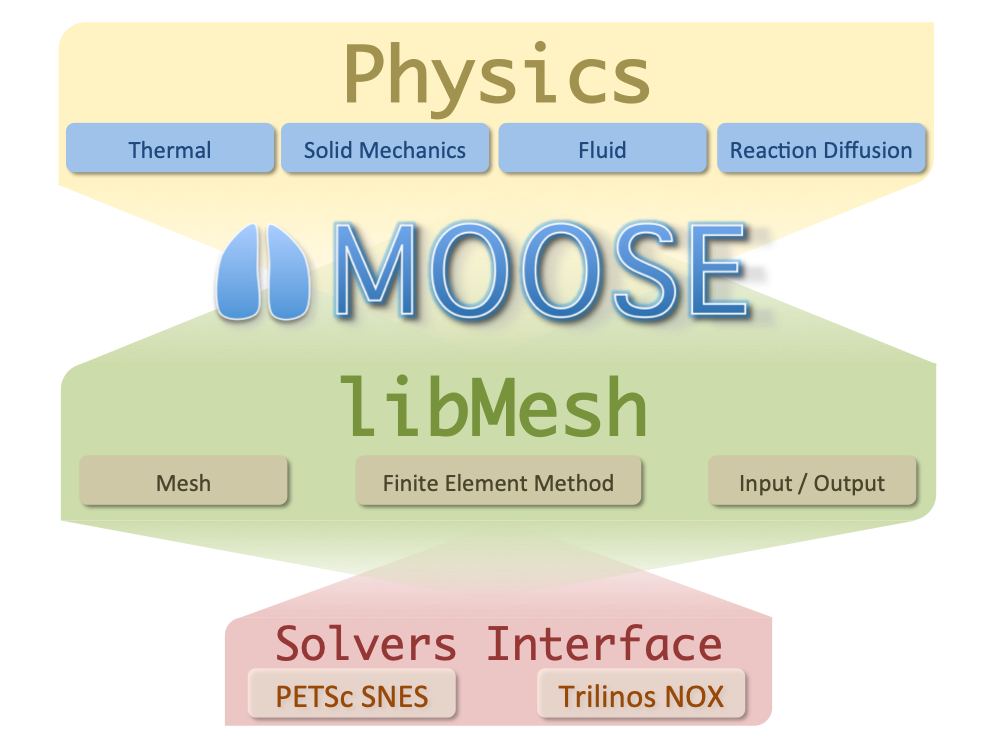
\includegraphics[width=.7\columnwidth]{moose}
	\caption{Structure of MOOSE and its dependencies.}
	\label{fig:moose}
\end{figure}

MOOSE relies on two other open-source libraries: libMesh
\cite{kirk_libmesh_2006} for its \gls{FEM} capabilities on unstructured mesh
and PETSc \cite{satish_petsc_2019} for its nonlinear solvers and
preconditioning routines. By extension, Moltres gains access to these
sophisticated numerical analysis tools and benefits from their continuous
development. Figure
\ref{fig:moose} shows how MOOSE serves as an interface between physics
applications and libMesh/PETSc. MOOSE supports
modeling on up to three-dimensional (3-D) unstructured meshes for a wide range
of mesh file formats, including the commonly used Exodus II file format. For
2-D meshes, users can opt between Cartesian and polar RZ coordinates. MOOSE
also supports parallel computing through the \gls{MPI} library to leverage
modern high-performance computing for large multiphysics simulations.

Moltres benefits from the highly-integrated cross compatibility within the
ecosystem of MOOSE-based applications. MOOSE facilitates multiphysics coupling
among all MOOSE-based applications by providing a common framework for shared
data access and file input/output, thus eliminating computational costs from
data transfers and allowing for fully coupled simulations. For example, Moltres
can couple with the \texttt{Navier-Stokes} module \cite{peterson_overview_2018}
from MOOSE for fully coupled reactor simulations modeling neutronics and
thermal-hydraulics with incompressible flow modeling. Section
\ref{sec:msr-multiphysics} highlighted the advantages of fully coupled schemes
for modeling strongly coupled systems, such as the coupled
neutronics and thermal-hydraulics in \glspl{MSR}. Moltres can also easily
couple to other MOOSE-based applications in a similar fashion. In
addition, MOOSE
provides the option for either tight or loose coupling through the
\texttt{MultiApp} system \cite{gaston_physics-based_2015}. Tight coupling
schemes can outperform fully coupled schemes in weakly coupled systems in which
the computational expenses of fully coupled schemes outweigh the savings from
running fewer Newton iterations due to the superior convergence rate. Loose
coupling schemes help accelerate time-dependent simulations of
stable systems towards a steady state if only the steady-state
configuration interests the user. This situation may occur in the later
stages of \gls{MSR} simulations when the \gls{DNP}
concentrations converge slowly due to their relatively large decay half-lives.
Furthermore, segregated solvers through the \texttt{MultiApp} system enable
Moltres to introduce \gls{DNP} drift and non-uniform
temperature distributions into criticality search simulations. Regardless of
which coupling scheme works best, MOOSE-based applications provide the flexibility
to switch among the schemes as users see fit. For time-dependent simulations,
MOOSE provides more than ten implicit and explicit timestepping
schemes. The default scheme is the first-order backward Euler
method which offers excellent solver stability for stiff \glspl{PDE}.

Lastly, Moltres is an open-source \gls{LGPL} software hosted on
GitHub \cite{github_build_2017}. Open-sourcing software provides ease of access
and expands the user base. These characteristics promote software quality
through increased feedback on users' needs and transparency for peer review.
Open-source software accelerate research progress by supporting
collaboration and sharing best software practices. Supporting Moltres'
continued development, Moltres relies on GitHub for online version control with
continuous integration testing to protect its existing capabilities.

In summary, Moltres provides robust and flexible coupling capabilities to
model strongly coupled neutronics and thermal-hydraulics in \glspl{MSR}. As a
MOOSE-based application, Moltres is highly extensible through coupling with
other MOOSE-based applications and benefits from MOOSE's user-friendly
interface for software development and general ease of use.

\subsection{Physics Models} \label{sec:moltres-physics}

This section describes the various physics models available in Moltres to model
coupled neutronics and thermal-hydraulics in \glspl{MSR}. Section \ref{sec:nts}
discusses the neutronics model in Moltres, Section \ref{sec:th} discusses
the thermal-hydraulics model, and Section \ref{sec:moltres-loop} discusses the
external loop model for \gls{DNP} looping and heat removal via external heat
exchangers.

\subsubsection{Multigroup Neutron Diffusion Model} \label{sec:nts}

Moltres solves the multigroup neutron diffusion equations for the neutron
flux solution within the problem domain. These equations are derived from the
neutron transport equation in the diffusion-dominated limit with Fick's law of
diffusion. They are further simplified by discretizing the continuous neutron energy
variable into a finite number of energy groups \cite{bell_nuclear_1970,
duderstadt_nuclear_1976}. The time-dependent multigroup neutron
diffusion equations with $G$ energy groups and $I$ \gls{DNP}
groups are given by:
%
\begin{align}
    \frac{1}{v_g} \frac{\partial \phi_g}{\partial t} =& \nabla \cdot D_g
    \nabla \phi_g - \Sigma^r_g \phi_g +
    \sum^G_{g' \neq g} \Sigma^s_{g' \rightarrow g} \phi_{g'} \nonumber \\
    &+ \chi^p_g \sum^G_{g'=1} \left( 1-\beta \right) \nu \Sigma^f_{g'}
    \phi_{g'} + \chi^d_g \sum^I_i \lambda_i C_i \label{eq:neutron} %\\
    %
    \shortintertext{where}
    v_g =& \text{ average speed of neutrons in group $g$,} 
    \nonumber \\
    \phi_g =& \text{ neutron flux in group $g$,}
    \nonumber \\
    t =& \text{ time,} \nonumber \\
    D_g =& \text{ diffusion coefficient of neutrons in group $g$,} \nonumber \\
    \Sigma^r_g =& \text{ macroscopic removal cross section for} \nonumber \\
    &\text{ neutrons from group $g$,} \nonumber \\
    \Sigma^s_{g' \rightarrow g} =& \text{ macroscopic scattering cross section
    for neutrons from} \nonumber \\
    &\text{ groups $g'$ to $g$,} \nonumber \\
    \chi^p_g =& \text{ prompt fission spectrum for neutrons in group $g$,} \nonumber \\
    G =& \text{ total number of discrete neutron groups,} \nonumber \\
    \nu_g =& \text{ average number of neutrons produced per fission,} \nonumber
    \\
    \Sigma^f_{g} =& \text{ macroscopic fission cross section for neutron}
    \nonumber \\
    &\text{ in group $g$,} \nonumber \\
    \chi^d_g =& \text{ delayed fission spectrum for neutrons in group $g$,} \nonumber \\
    I =& \text{ total number of \gls{DNP} groups,} \nonumber \\
    \beta =& \text{ total delayed neutron fraction.} \nonumber
\end{align}

Despite forming only around 0.7\% of all neutrons emitted, delayed neutrons
play outsized roles in reactor kinetics. The relatively long half-lives of
\glspl{DNP} give reactor operators ample time in adequately designed reactors
to control reactor power output and intervene in case of power excursions.
The precursor concentration balance equations for $I$ precursor
groups are given by:
%
\begin{align}
    \frac{\partial C_i}{\partial t} =& \beta_i \sum^G_{g'=1} \nu \Sigma^f_{g'}
    \phi_{g'} - \lambda_i C_i - \vec{u} \cdot \nabla C_i + \nabla \cdot
    D_{\text{P}} \nabla C_i \label{eq:precursor} %\\
    %
    \shortintertext{where}
    \beta_i =& \text{ delayed neutron fraction of precursor group $i$,}
    \nonumber \\
    \lambda_i =& \text{ average decay constant of delayed neutron} \nonumber \\
    &\text{ precursors in precursor group $i$,} \nonumber \\
    C_i =& \text{ concentration of \gls{DNP}s in}
    \nonumber \\
    &\text{ precursor group $i$,} \nonumber \\
    \vec{u} =& \text{ molten salt flow velocity vector,}
    \nonumber \\
    D_{\text{P}} =& \text{ effective diffusion coefficient of the delayed}
    \nonumber \\
    &\text{ neutron precursors.} \nonumber
\end{align}

These two equations are largely similar to conventional formulations of the
multigroup neutron diffusion equations with delayed neutrons for most reactor
types. The only differences are in the last two terms in Equation
\ref{eq:precursor}
which represent the advection and diffusion terms, respectively, to model the
movement of \glspl{DNP} in liquid-fuel \glspl{MSR}.

As shown in Equations \ref{eq:neutron} and \ref{eq:precursor}, Moltres requires
group constant data from dedicated high-fidelity neutronics software such as
the NEWT module in SCALE \cite{dehart_reactor_2011}, Serpent
\cite{leppanen_serpent_2014}, or OpenMC \cite{romano_openmc:_2015}. These group
constant data are the neutron energy group $g$ values for $v_g$, $D_g$,
$\Sigma^r_g$, $\Sigma^s_{g' \rightarrow g}$, $\chi^p_g$, $\chi^d_g$,
$\Sigma^f_{g}$, and $\nu\Sigma^f_{g}$, and precursor group $i$ values for
$\beta_i$ and $\lambda_i$. Users
can run a Python script in Moltres' Github repository, which automatically reads
user-provided SCALE/Serpent/OpenMC output data files and creates
Moltres-compatible JSON format files containing all required group constant
data. Moltres allows for an arbitrary number of neutron energy groups $G$ and
precursor groups $I$ as long as the user provides the necessary group constant
data. In practice, $I$ depends on the nuclear data library used to generate
group constants---the JEFF \cite{plompen_joint_2020} and ENDF
\cite{brown_endfb-viii0_2018} data libraries define eight precursor groups
and six precursor groups, respectively.

In multiphysics reactor simulations, we model the coupling between neutronics
and thermodynamics through temperature-dependent group constants. To sample
group constants at different temperatures in Moltres, users must provide group
constant data measured at more than one temperature (e.g., 800K--1500K at 100K
intervals). Users can then choose from linear spline, cubic spline, or monotone
cubic interpolation methods available in Moltres to interpolate the group
constant data for values falling within the provided temperature range. 

Moltres provides two types of boundary conditions for neutron fluxes; these are
conventionally known as the vacuum and reflective boundary conditions given,
respectively, as:

\begin{align}
  D_g \nabla \phi_g \cdot \hat{n} + \frac{\phi}{2} =& 0 \label{eq:vacuum}
    \shortintertext{and}
  \nabla \phi \cdot \hat{n} =& 0
    \shortintertext{where}
  \hat{n} =& \mbox{ outward unit normal vector to the boundary.} \nonumber
\end{align}

The vacuum boundary condition typically applies to the external boundaries of
the reactor beyond which lies low-interaction media such as air. The
reflective boundary condition is useful for exploiting symmetries in the
model geometry, such as along the axial boundary in axisymmetric geometries. The
reflective boundary condition is equivalent to the more generally known
homogeneous Neumann boundary condition. Relevant boundary conditions for
\glspl{DNP} include the homogeneous Neumann boundary condition
along fuel salt-structural interfaces and outflow/inflow boundary
conditions along the outlet/inlet boundaries through which the precursors
flow as they circulate the fuel salt loop.

\subsubsection{Incompressible Flow Model} \label{sec:th}

Moltres relies on MOOSE's \texttt{Heat} \texttt{Conduction} and
\texttt{Navier-Stokes} physics modules for its thermal-hydraulics modeling
capabilities. While the \texttt{Navier-Stokes} module supports
compressible and incompressible flow modeling, this work focuses on
multiphysics coupling in \glspl{MSR} with the latter. The
time-dependent incompressible Navier-Stokes equations for velocity $\vec{u}$
with the Boussinesq approximation for buoyancy-driven flow are given as:

\begin{align}
    \text{Momentum equation: } \rho \frac{\partial \vec{u}}{\partial t} =&
    -\rho (\vec{u}
    \cdot \nabla) \vec{u} - \nabla p + \mu \nabla^2 \vec{u}
    + \rho \alpha \vec{g} \left(T - T_{\text{ref}} \right)
    \label{eq:momemtum}
    \shortintertext{and}
    \text{Mass equation: } \nabla \cdot \vec{u} =& 0
    \label{eq:divergence}
    \shortintertext{where}
    \rho =& \text{ fluid density,} \nonumber \\
    p =& \text{ pressure,} \nonumber \\
    \mu =& \text{ dynamic viscosity,} \nonumber \\
    \alpha =& \text{ coefficient of thermal expansion,} \nonumber \\
    \vec{g} =& \text{ gravitational force vector,} \nonumber
    \\
    T =& \text{ fluid temperature,} \nonumber \\
    T_{\text{ref}} =& \text{ reference temperature at which the nominal}
    \nonumber \\
    &\text{ density is provided.} \nonumber
    \nonumber
\end{align}

Velocity variables and advected quantities such as temperature are susceptible
to numerical node-to-node oscillations
commonly observed when resolving advection-dominated flows using continuous
Galerkin methods \cite{kuhlmann_lid-driven_2018}. The \texttt{Navier-Stokes}
module provides the \gls{SUPG} stabilization scheme
\cite{brooks_streamline_1982} for the velocity and temperature variables to
minimize these oscillations. The module also provides the \gls{PSPG}
stabilization scheme \cite{hughes_new_1986}, enabling equal-order
discretizations of pressure and velocity. Peterson et al. \cite{peterson_overview_2018}
provide further detail on the implementation of these stabilization schemes in
the \texttt{Navier-Stokes} module.

\subsubsection{Temperature Advection-Diffusion Model}

Lastly, Moltres solves for the temperature distribution through the temperature
advection-diffusion equation given by:

\begin{align}
    \rho c_{p} \frac{\partial T}{\partial t} =& - \rho c_p \vec{u}
    \cdot \nabla T + \nabla \cdot \left(k \nabla T \right) + Q_f - Q_s
    \label{eq:temp}
    \shortintertext{and}
    Q_f =& \sum^G_{g=1} \epsilon_g \Sigma_g^f \phi_g \label{eq:heat-source}
    \shortintertext{where}
    c_p =& \text{ specific heat capacity of molten salt,} \nonumber \\
    k =& \text{ effective thermal conductivity of molten salt,} \nonumber \\
    Q_f =& \text{ fission heat source,} \nonumber \\
    \epsilon_g =& \text{ average fission energy released by neutrons in group
    $g$,} \nonumber \\
    Q_s =& \text{ heat sink/removal.} \nonumber
\end{align}

$Q_f$ represents the fission heat source term and is calculated by taking the
sum of neutron group fluxes multiplied by their respective macroscopic fission
cross sections and the average fission energy released per fission.

The \texttt{Navier-Stokes} module provides the following types of boundary
conditions for the velocity and temperature variables:

\begin{align}
    \text{Dirichlet: }& & u \ \left(\text{or } T\right) =& c & \\
    \text{Homogeneous Neumann: }& & \frac{\partial u}{\partial x_i} \
    \left(\text{or } \frac{\partial T}{\partial x_i}\right) =& 0 & \\
    \text{``No boundary condition'' outflow: }& &
    \left[ \nabla \vec{u} + \left(\nabla \vec{u} \right)^T \right] \cdot
    \hat{n} =& 0 \ \text{ (velocity)} & \\
    \text{``No boundary condition'' outflow: }& &
    k \nabla T \cdot\hat{n} =& 0 \ \text{ (temperature)} &
    \shortintertext{where}
    & & c =& \text{ user-defined constant value,} & \nonumber \\
    & & \hat{n} =& \text{ unit normal vector to the boundary.} & \nonumber
\end{align}

The Dirichlet boundary condition can be used to set the inlet velocities and
temperatures and no-slip conditions along solid boundaries. The
homogeneous Neumann boundary condition is commonly
imposed along the outlet boundary. However, the latter approach
artificially influences upstream behavior, especially in developing flow. The
``no boundary condition'' outflow boundary condition by Griffiths
\cite{griffiths_no_1997} has been shown to reduce such upstream errors.

\subsubsection{External Loop Model} \label{sec:moltres-loop}

Moltres also accounts for the decay of
\glspl{DNP} outside the active core region by simulating its flow in a
separate 1-D pipe geometry. This external loop pipe calculation is tightly
coupled to the active core simulation through Picard iterations in MOOSE's
MultiApp \cite{gaston_physics-based_2015} functionality and inlet/outlet boundary values.
The external loop region is assumed to be subcritical to minimize neutron
irradiation upon heat exchangers, pumps, and other equipment. Therefore, the
only significant neutronic-related phenomena are the drift and decay of
\glspl{DNP}. The governing equation for the \glspl{DNP} is:
%
\begin{align}
    \frac{\partial C_i}{\partial t} =& - \lambda_i C_i - u
    \frac{\partial C_i}{\partial x}.
    \label{eq:dnploop}
\end{align}
%
Equation \ref{eq:dnploop} is derived from equation \ref{eq:precursor} by
removing the fission \gls{DNP} source and diffusion terms and reducing the
dimensionality from 3-D to 1-D.

Moltres also simulates the temperature distribution in the external loop to model heat removal via
heat exchangers. The governing equation
for temperature, derived from equation \ref{eq:temp}, is:
%
\begin{align}
    \rho c_{p} \frac{\partial T}{\partial t} =& - \rho c_p u
    \frac{\partial T}{\partial x} - Q_{hx} \label{eq:temploop}
    \shortintertext{where}
    Q_{hx} =& \text{heat removal rate through the heat exchanger.} 
    \nonumber
\end{align}
%
The fission heat source term is replaced with a heat
exchanger sink term $Q_{hx}$.

Table \ref{table:loopbc} lists the boundary conditions for all variables on the inlet and outlet of
the 1-D external loop region. The inlet boundary conditions are all Dirichlet boundary conditions. The
prescribed value for the inlet boundary conditions are set to match the average outflow from the
active core region. The outlet boundary conditions are all outflow boundary conditions, as shown in
Table \ref{table:loopbc}.

\begin{table}[htbp!]
    \small
	\caption{Boundary conditions in the 1-D external loop geometry. $u$
	represents the 1-D velocity in this region.}
	\centering
	\begin{tabular}{ l l c}
		\toprule
		Variable & Boundary & Boundary Condition \\
        \midrule
        \multirow{2}{*}{Delayed neutron precursor concentration $C_i$} &
        Inlet (Core) & $C_i = c$ \\
        & Outlet (Core) & $u \cdot C_i = 0$ \\
        \midrule
        \multirow{2}{*}{Temperature $T$} &
        Inlet (Core) & $T = c$ \\
        & Outlet (Core) & $u \cdot T = 0$ \\
		\bottomrule
	\end{tabular}
	\label{table:loopbc}
\end{table}

\subsubsection{Core and External Loop Coupling Model}

This subsection details the \gls{DNP} and
temperature coupling between the core and external loop regions. 

At every timestep, Moltres calculates weighted averages of the
temperature and the precursors at the outlet. These values are weighted by the
outflow velocity values at the outlet according to the following equation:
%
\begin{align}
    \overline{\psi} =& \frac{\int_\mathcal{C} Y(x_j) u(x_j) dx_j}{
    \int_\mathcal{C} u(x_j) dx_j} \\
    \shortintertext{where}
    Y =& \text{ variable to be weighted} \nonumber \\
    \mathcal{C} =& \text{ outlet boundary area} \nonumber \\
    u =& \text{ outflow velocity perpendicular to the outlet boundary,} \nonumber \\
    x_j =& \text{ spatial coordinate parallel to the outlet boundary.}
    \nonumber
\end{align}

Moltres transfers this outflow value from the core region to the 1-D
external loop region to be used as the boundary value for the inhomogeneous
Dirichlet boundary
condition at the inlet. Likewise, the outflow value from the external
loop region is used for the inflow value in the central core region. No
averaging is required for this step as the external loop region is a 1-D system.
This approach results in uniform inflow temperature and \gls{DNP} at the
inlet. The Picard iterations within every timestep ensure the two systems
are tightly coupled.

\subsection{Previous \gls{MSR} Analyses with Moltres} \label{sec:moltres-previous}

This section discusses some previous work with Moltres to illustrate its
various capabilities and coupling approaches for multiphysics \gls{MSR}
modeling and simulation. Section \ref{sec:msre} summarizes the work by Lindsay et
al. \cite{lindsay_introduction_2018} in modeling the \gls{MSRE}, and Section
\cite{park_advancement_2020} summarizes my previous work in modeling the
\gls{MSFR}.

\subsubsection{Introduction to Moltres and Modeling the MSRE} \label{sec:msre}

This section follows the work by Lindsay et al. in \textit{Introduction to Moltres:
An Application for Simulation of Molten Salt Reactors}
\cite{lindsay_introduction_2018}.

In 2017, Lindsay et al. introduced
Moltres to the \gls{MSR} community for multiphysics simulations of \glspl{MSR}.
Their work showcased neutron diffusion and thermal-hydraulics coupling
capabilities in Moltres. The authors
demonstrated these capabilities by running time-dependent simulations of 2-D
axisymmetric and 3-D \gls{MSRE} models until the flux, precursor, and
temperature distributions reached a steady state.

\begin{figure}[htb!]
	\centering
	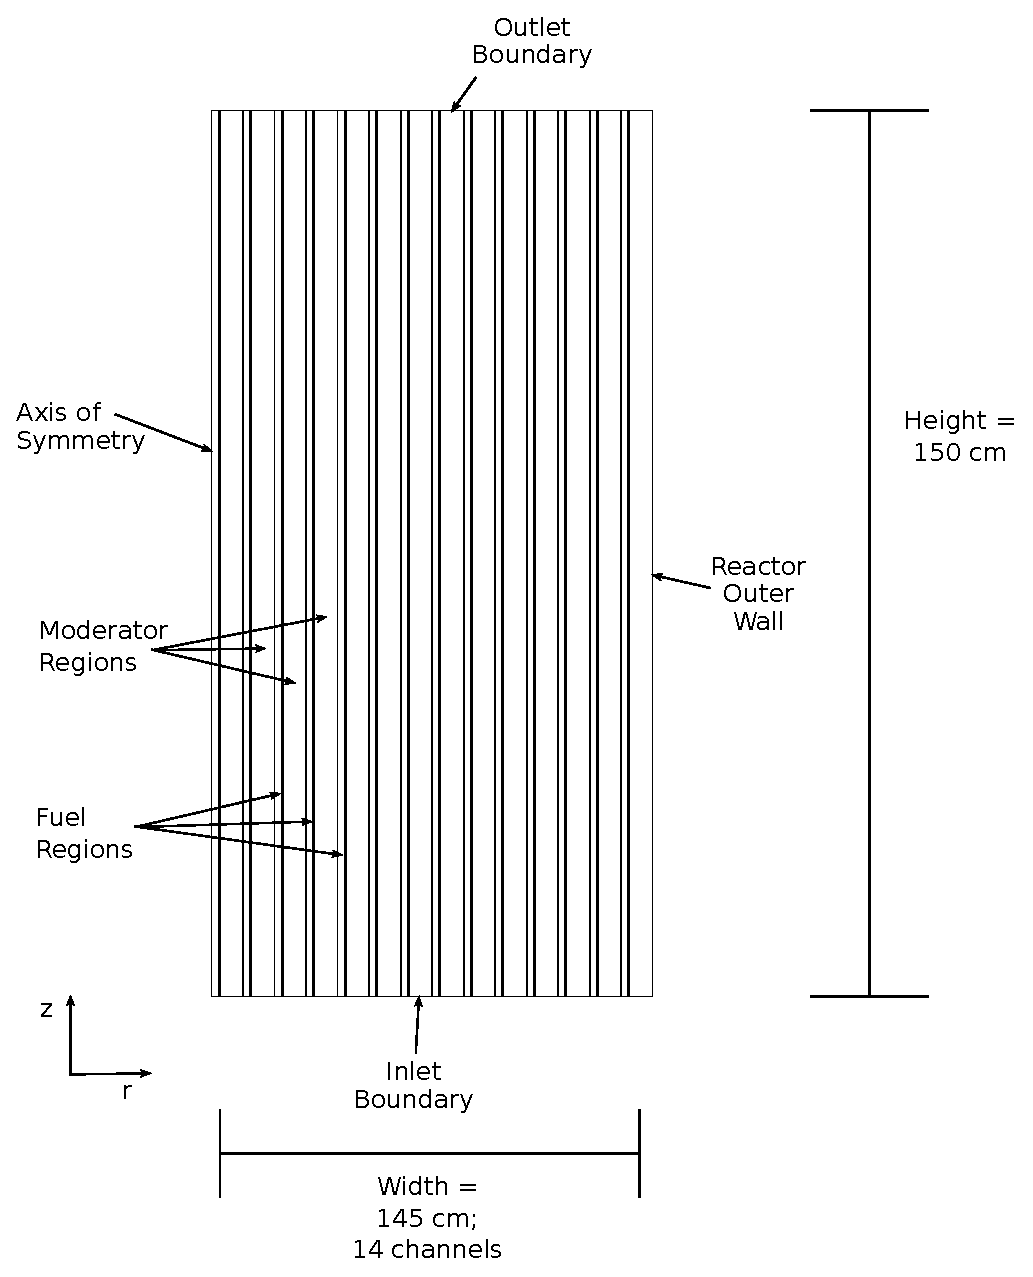
\includegraphics[width=.45\columnwidth]{msre-geometry}
	\caption{Schematic diagram of the 2-D axisymmetric \gls{MSRE} geometry
	adopted by Lindsay et al. \cite{lindsay_introduction_2018}.}
	\label{fig:msre-geometry}
\end{figure}

Figure \ref{fig:msre-geometry} shows the fuel channels and moderator regions of
the 2-D \gls{MSRE} geometry that Lindsay et al. adopted for their study.
They ran a two-group neutron diffusion model with six precursor groups and
vacuum boundary conditions on the outer boundaries governed by Equations
\ref{eq:neutron}, \ref{eq:precursor}, and \ref{eq:vacuum} shown in Section
\ref{sec:nts}. They modeled precursor drift due to fuel salt flow by imposing
fixed uniform flow upwards through the fuel channels shown in Figure
\ref{fig:msre-geometry}. Their thermal-hydraulics model employed a
governing equation for temperature in the fuel salt equivalent to Equation
\ref{eq:temp} with fixed uniform flows while imposing a cosine-shaped heat
source term representing heat dissipation from gamma and neutron irradiation in
the graphite moderator region. In addition, all governing equations were fully
coupled and solved simultaneously as a single system of equations with implicit
Euler timestepping to accurately and efficiently resolve the strong coupling
expected between the neutronics and temperature.

\begin{figure}[htb!]
	\centering
	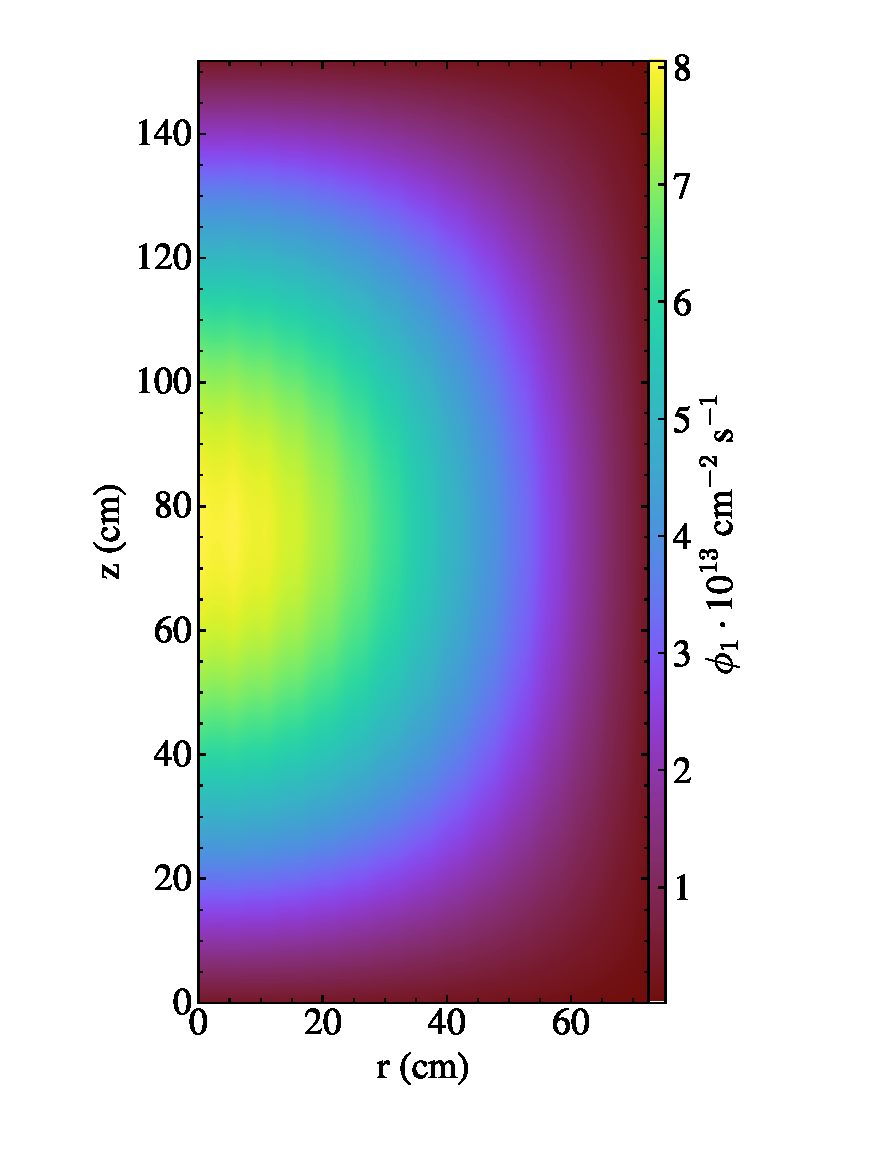
\includegraphics[width=.45\columnwidth]{2d_gamma_heating_group1}
	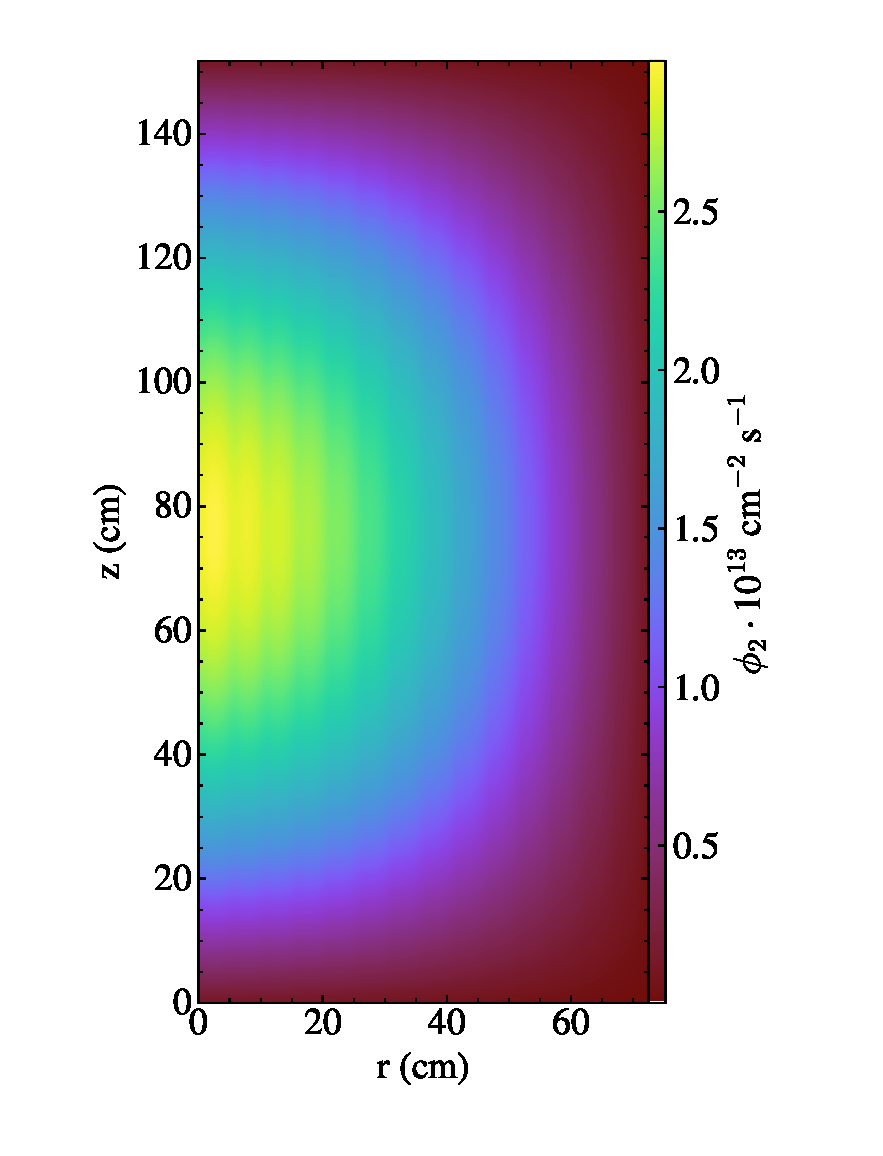
\includegraphics[width=.45\columnwidth]{2d_gamma_heating_group2}
	\caption{Neutron group 1 and 2 fluxes in the 2-D axisymmetric \gls{MSRE}
	model from Lindsay et al. \cite{lindsay_introduction_2018}.}
	\label{fig:msre-flux}
\end{figure}

\begin{figure}[htb!]
	\centering
	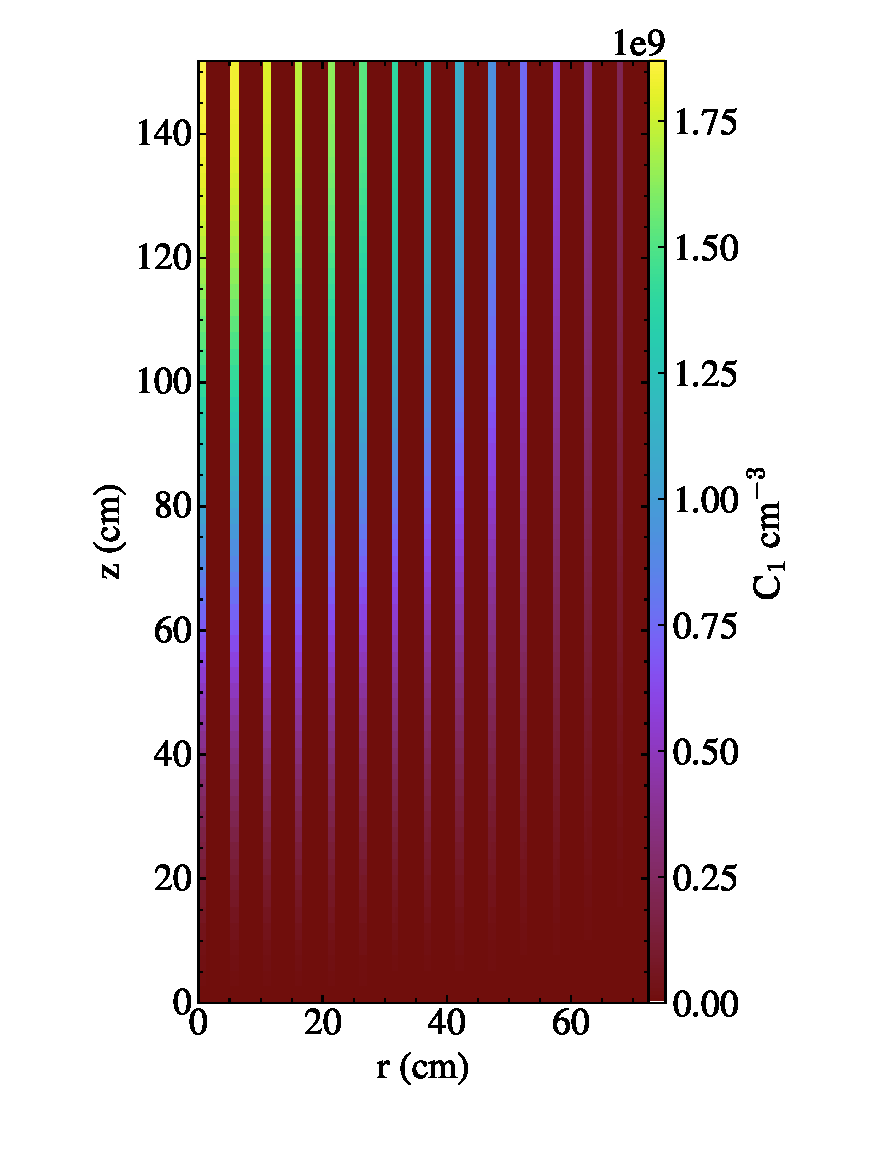
\includegraphics[width=.45\columnwidth]{2d_gamma_heating_pre1_scaled}
	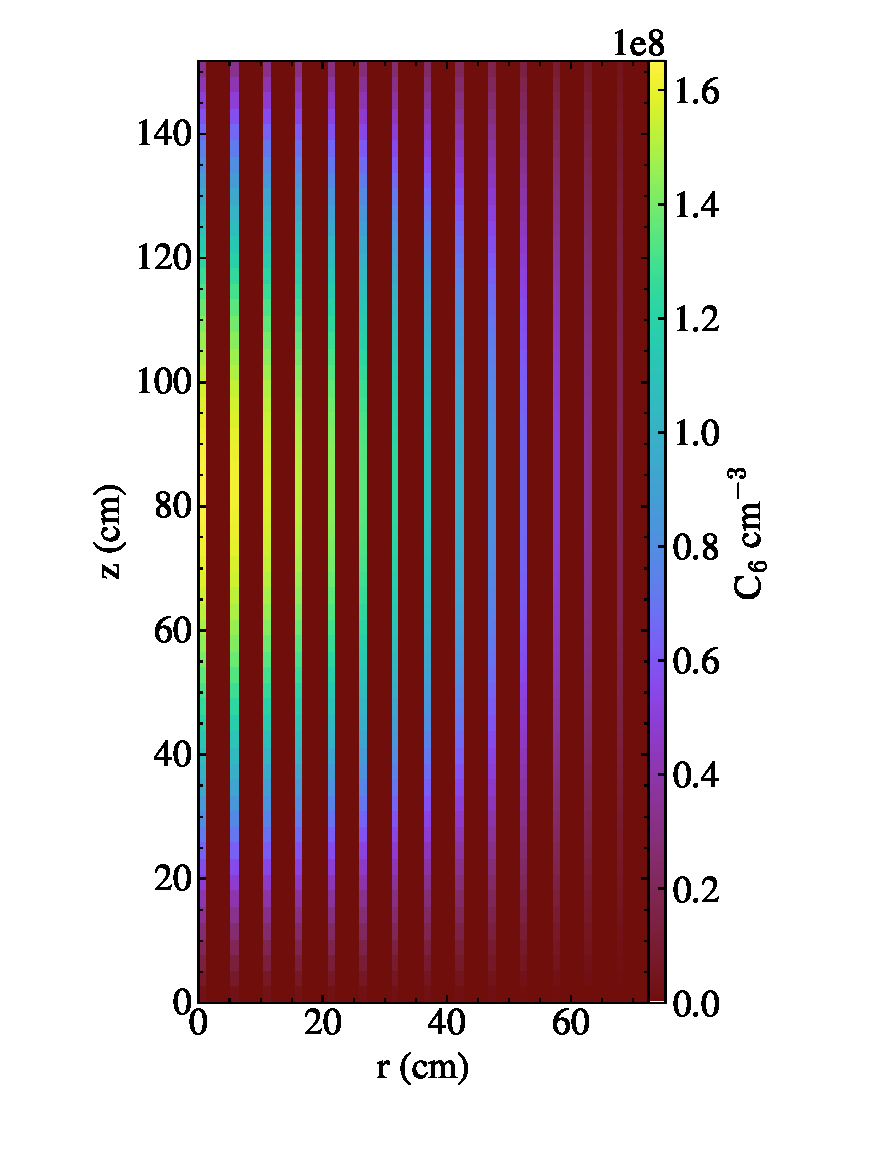
\includegraphics[width=.45\columnwidth]{2d_gamma_heating_pre6_scaled}
	\caption{Longest- and shortest-lived precursor concentrations ($\lambda =
	1.24\times 10^{-2}$s$^{-1}$ and $3.07$s${-1}$, respectively) in the 2-D
	axisymmetric \gls{MSRE} model from Lindsay et al.
	\cite{lindsay_introduction_2018}.}
	\label{fig:msre-precursor}
\end{figure}

\begin{figure}[htb!]
	\centering
	\begin{minipage}[b]{0.45\columnwidth}
	    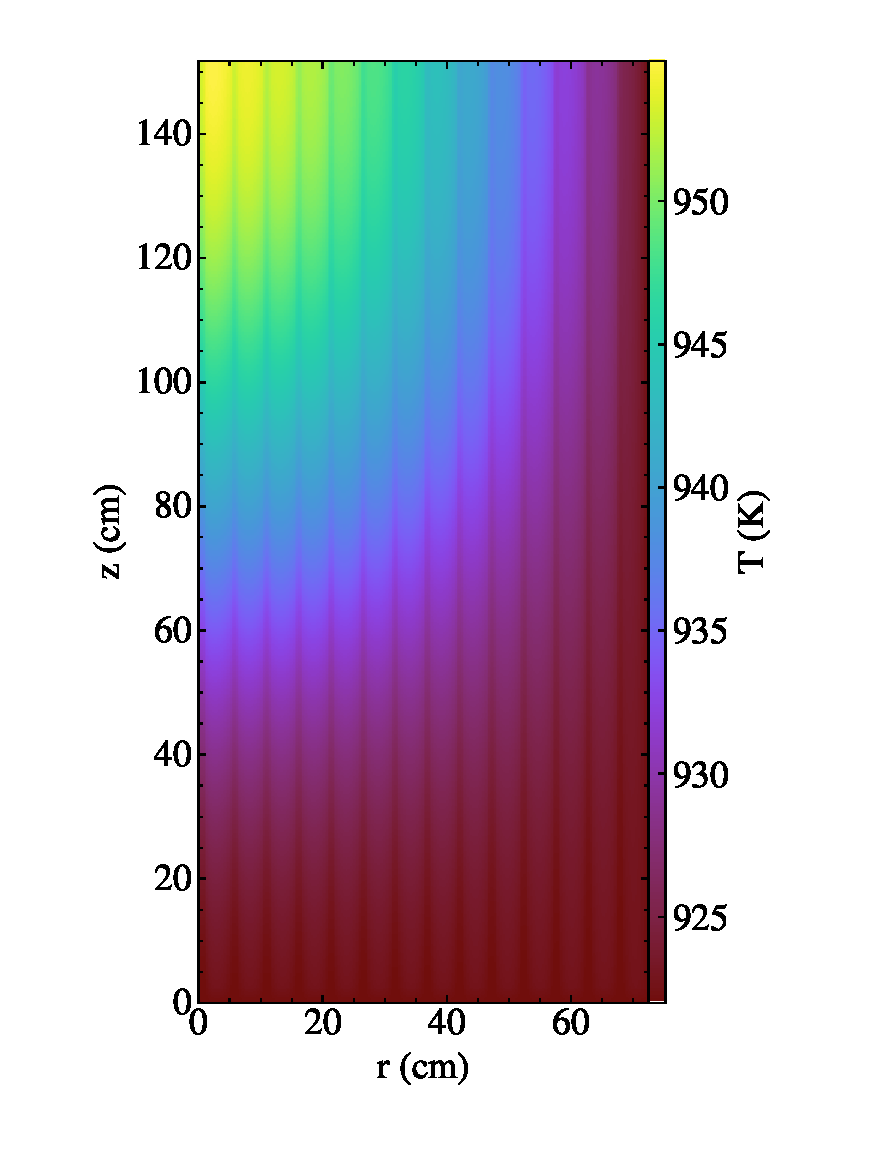
\includegraphics[width=\columnwidth]{2d_gamma_heating_temp}
	    \caption{Temperature distribution in the 2-D
	    axisymmetric \gls{MSRE} model from Lindsay et al.
	    \cite{lindsay_introduction_2018}.}
	    \label{fig:msre-temp}
	\end{minipage}
	\hfill
	\begin{minipage}[b]{0.45\columnwidth}
	    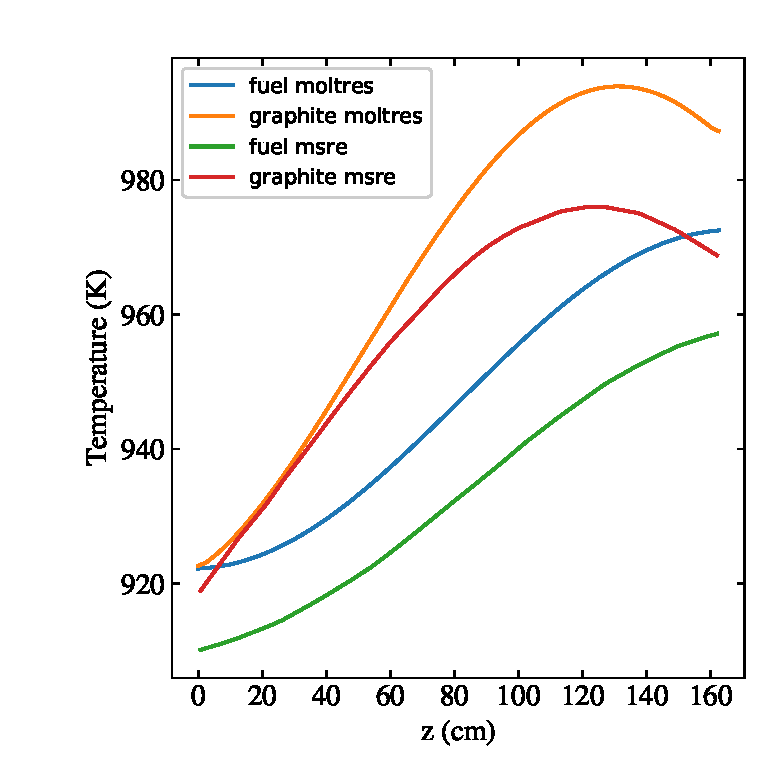
\includegraphics[width=\columnwidth]{combined_msre_moltres_axial_temps}
	    \caption{Moltres \cite{lindsay_introduction_2018} and \gls{ORNL}
	    \gls{MSRE} \cite{briggs_molten-salt_1964} axial temperature
	    distributions in the hottest fuel channel and adjacent graphite.}
	    \label{fig:msre-temp-plot}
	\end{minipage}
\end{figure}

Figure \ref{fig:msre-flux} shows the fast and thermal neutron fluxes
corresponding to group 1 and 2 in the 2-D \gls{MSRE} model. As expected, the
fluxes exhibit general cosine shapes in the axial and radial directions. We
also observe minor oscillations in the radial direction coinciding with the
regular fuel and moderator lattice. The fuel regions favor the fast flux, while
the moderator regions favor the thermal flux.

Figure \ref{fig:msre-precursor}
shows the longest- and shortest-lived precursor concentrations in the fuel
channels. With a long half-life of 55.9 s relative to the 6.91 s it takes for
salt to flow from bottom to top, the longest-lived precursor concentration peaks
outside the model domain. By contrast, the shortest-lived precursor
concentration closely follows the neutron fluxes' cosine shape, which
dictate where the precursors are born.

Finally, Figure \ref{fig:msre-temp}
shows the temperature distribution in the 2-D \gls{MSRE} model. The temperature
naturally peaks near the outlet due to upward advection. The moderator regions
experience hotter temperatures than the fuel regions due to radiative heating
and the relative inefficiency of heat conduction in the graphite compared to
advection in the fuel salt.

\begin{figure}[htb!]
	\centering
	\begin{subfigure}[h]{0.45\columnwidth}
	    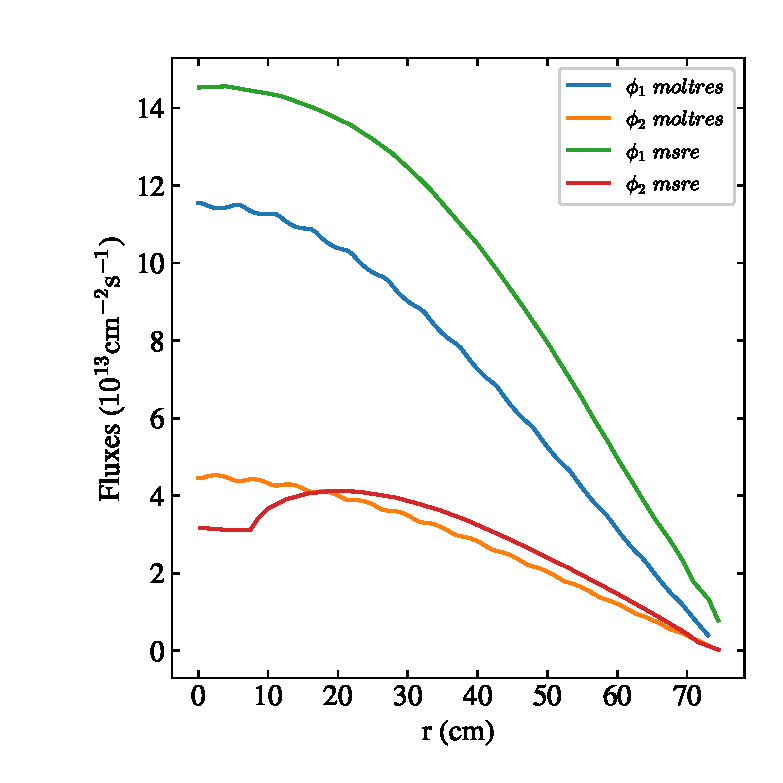
\includegraphics[width=\columnwidth]{combined_msre_moltres_radial}
	    \caption{Radial fluxes at reactor half-height.}
	    \label{fig:msre-flux-radial}
	\end{subfigure}
	\hfill
	\begin{subfigure}[h]{0.45\columnwidth}
	    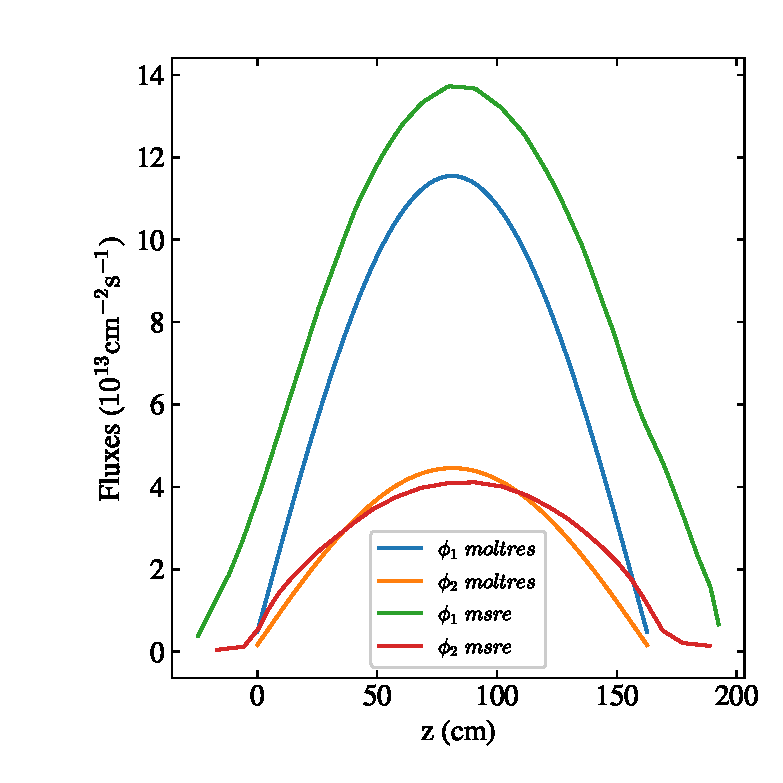
\includegraphics[width=\columnwidth]{combined_msre_moltres_axial}
	    \caption{Axial fluxes along the core centerline ($r=0$ cm).}
	    \label{fig:msre-flux-axial}
	\end{subfigure}
	\caption{The fast and thermal fluxes from
	Moltres \cite{lindsay_introduction_2018} and the \gls{ORNL} \gls{MSRE}
	design calculations \cite{briggs_molten-salt_1964}.}
\end{figure}

The corresponding neutronics and thermal-hydraulics results from their 3-D model
show good qualitative agreement with the 2-D results. Given the lack of
\gls{MSR} experimental data, they compared their 2-D model results with
\gls{MSRE} design calculations performed using legacy software in 1963-1964 at
\gls{ORNL}. Their neutron flux and temperature distribution results showed good
qualitative agreement with \gls{ORNL} data. The authors attributed
discrepancies to the following differences in the two modeling approaches: the
absence of axial heat conduction and the use of 32 neutron groups in the
\gls{ORNL} calculations, and the exclusion of control rod thimbles in the
Moltres calculations.

\paragraph{Critical Assessment} \label{sec:msre-critique}

Lindsay et al.'s work illustrated early development efforts for neutronics and thermal-hydraulics
models in Moltres. It demonstrated, along with advanced capabilities from the \gls{MOOSE}
framework, fully-coupled simulations of the \gls{MSRE} with implicit timestepping. The
decent qualitative agreement observed between Moltres and the \gls{ORNL}
\gls{MSRE} calculations proved that Moltres could simulate
\glspl{MSR} under some simplifying assumptions.

On the other hand, significant improvements could be made to Moltres to better
model multiphysics phenomena in \glspl{MSR}. For instance, replacing the
fixed uniform salt flow with a proper flow profile governed by fluid flow
equations would accurately capture precursor and temperature advection.
Temperature advection has a particularly large impact on the temperature
distribution in the fuel salt since molten salts generally have large Prandtl
numbers, which measure the ratio of convective to conductive heat transfer.
The flow-modeling feature would be of even greater importance when modeling
pool-type \glspl{MSR}, which consist of a single large fuel salt region in the
reactor core.

Another essential feature for modeling \glspl{MSR}, which was already under
development at the time of publication, is a precursor loop
system to recirculate precursors back into the core. While some precursors
decay outside the core, others survive long enough to recirculate back into the
core. The loop system would provide a more accurate estimate of the delayed
neutron fraction instead of discarding all precursors that flowed out of
the core. In transient simulations involving sudden increases in the neutron
flux, precursors recirculating into the core can induce observable jumps and
dips in the power output due to the associated reactivity insertion from the
delayed neutrons.

Moltres would also benefit from a decay heat model which Lindsay
et al. mentioned in their work \cite{lindsay_introduction_2018},
especially for transient accident analyses. While decay heat from fission
product decays represents a small fraction ($\sim5\%$) of total power output,
this heat source can be significant in unprotected loss of flow or loss of
secondary cooling accidents. Therefore, understanding residual heat generation
from fission product decays in \gls{MSR} is essential in preventing further
structural failure after an accident.

Specific to reactor physics modeling, Moltres also requires an accurate method for modeling
control rods. As observed in Figure \ref{fig:msre-flux}, the omission of control rods led to
significant discrepancies in the thermal flux distribution. However, developing control rod
modeling capability in Moltres is nontrivial given that neutron diffusion theory performs poorly
within highly neutron-absorbing regions.

Lastly, the authors recognized two other avenues for future work: further \gls{VV} of Moltres'
capabilities by comparison
with more detailed experimental data and other modern \gls{MSR} modeling
efforts; and the study of transient simulation cases such as control rod
ejection, single channel blockage, loss of flow, and loss of secondary cooling.

\subsubsection{Advancements in Moltres and Transient Simulations of the MSFR}
\label{sec:msfr}

This section follows my previous work for my Master's degree in \textit{Advancement and
Verification of Moltres for Molten Salt Reactor Safety Analysis} \cite{park_advancement_2020},
which I shall refer to as ``this work'' in this subsection.

In many ways, this work represents a continuation of the work by Lindsay et al.
\cite{lindsay_introduction_2018} in developing Moltres as an \gls{MSR}
simulation tool. New features introduced include coupling the existing
neutronics and temperature equations to incompressible Navier-Stokes equations
to model flow dynamics, the precursor loop system, and the decay heat model.
I later demonstrated these features through steady-state and transient
simulations of a 2-D axisymmetric \gls{MSFR} model.

Moltres couples natively with the \texttt{Navier-Stokes} module in \gls{MOOSE} for
incompressible flow modeling capabilities. Section \ref{sec:th} describes the governing equations
for incompressible flow and temperature advection-diffusion.
The precursor loop model was developed to model
precursor recirculation into the core. The precursor loop system leverages
the \texttt{MultiApp} system in \gls{MOOSE} to couple a 1-D pipe model to the
core to simulate precursor flow outside the core. The core and the pipe models
are coupled via inlet and outlet boundary conditions, as detailed in Section
\ref{sec:moltres-loop}. The loop system can also accommodate a pointwise heat
exchanger model with a heat removal rate as a function of time
or auxiliary variables in the Moltres simulation.

In addition, I developed a decay heat model to simulate delayed heat release
from the decay of fission products, similar to delayed neutron emission
from precursors. The decay heat model introduces decay heat groups of different
decay constants and variables representing the decay heat groups and modifies the
heat source term given by Equation \ref{eq:heat-source} to account for
the delayed heat generation. 

The number of decay heat groups depends on
the decay heat profile of the reactor after a specified period of operation.
Determining the decay heat profile requires fuel depletion calculations to
obtain the fuel composition during/after reactor operation and subsequent
calculations for the cumulative decay heat released from individual isotopes.
In this work, I cited results by Aufiero et al. \cite{aufiero_extended_2013},
who determined that three decay heat groups ($J=3$) were sufficient to
reproduce the decay heat profile of the \gls{MSFR} equilibrium fuel composition
for up to 300 seconds after shutdown with a relative error of less than 2\%.

\begin{figure}[htb!]
	\centering
	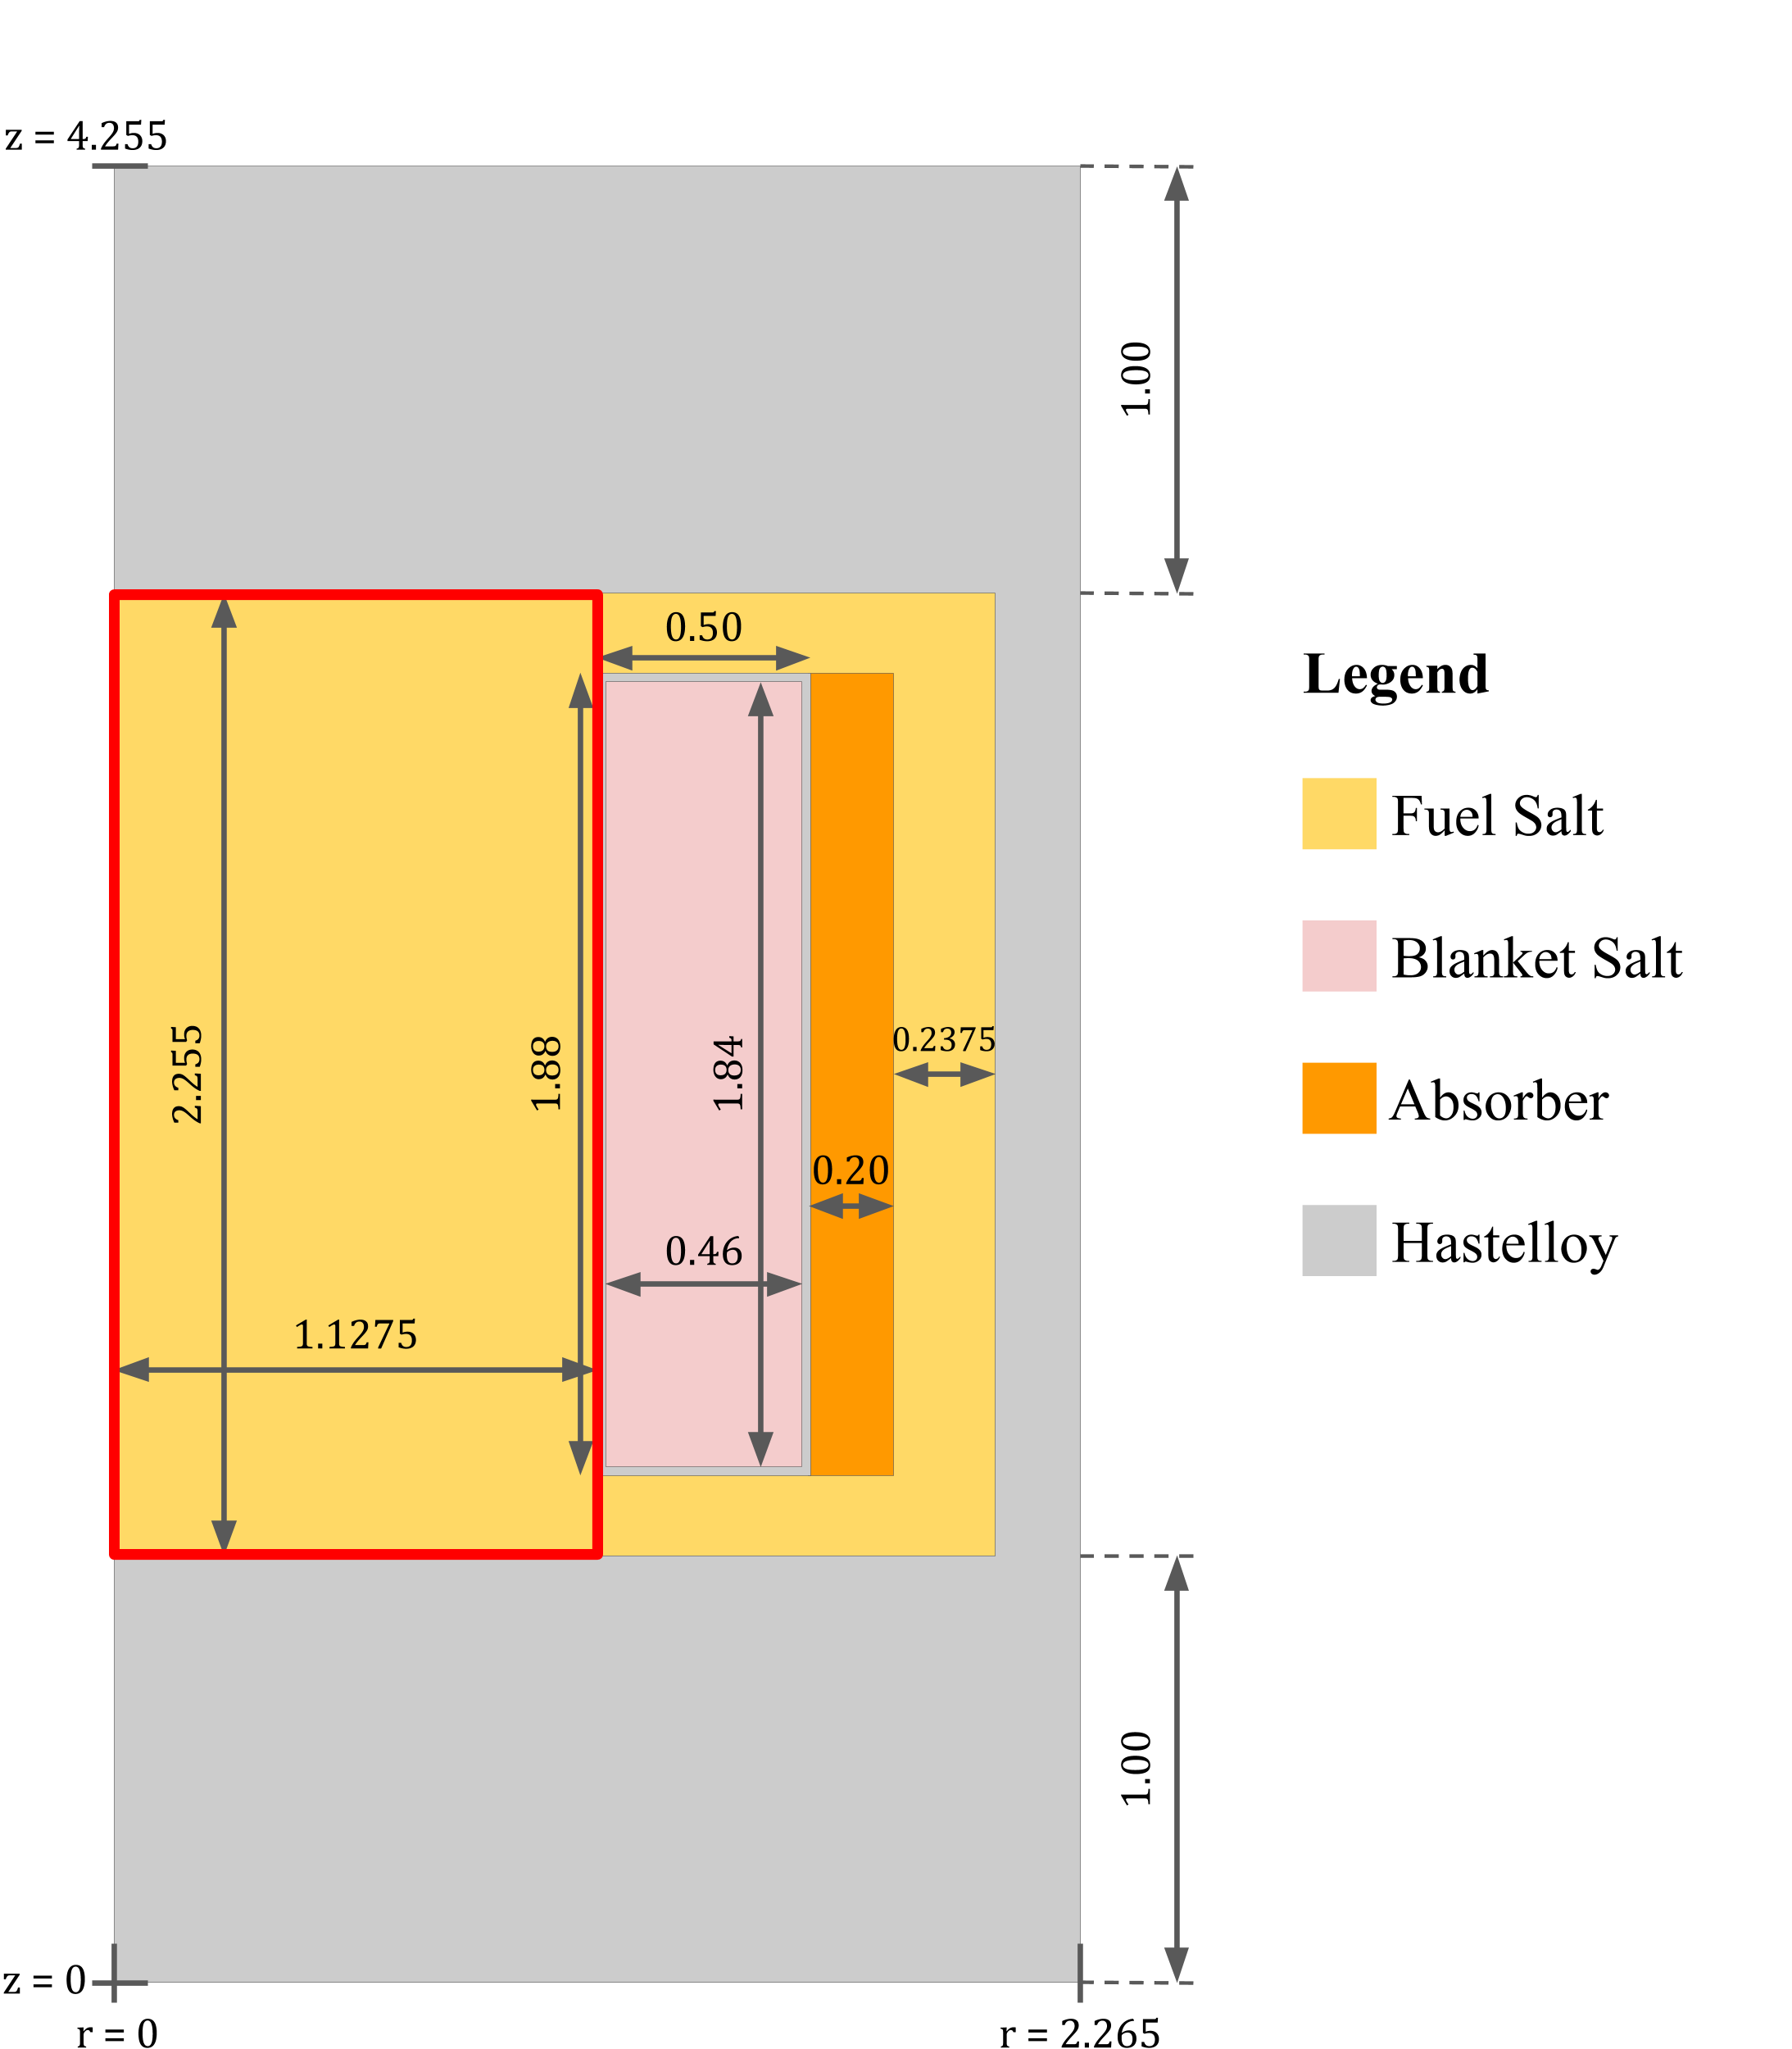
\includegraphics[width=.55\columnwidth]{central-core-legend}
	\caption{Schematic diagram of the 2-D axisymmetric \gls{MSFR} model with
	the core region enclosed by the red box \cite{park_advancement_2020}.}
	\label{fig:msfr-geometry}
\end{figure}

For the verification and demonstration of the capabilities introduced in this
work, I ran coupled steady-state and unprotected accident transient
simulations of the \gls{MSFR} and compared the results with published results
by Fiorina et al. \cite{fiorina_modelling_2014} and Aufiero et al.
\cite{aufiero_development_2014}. In this section, the PoliMi and TU Delft models
refer to two sets of results published by Fiorina et al. I compensated for
the lack of a turbulence model in Moltres by imposing a fixed turbulent
viscosity of 40 Pa$\cdot$s in addition to the molecular viscosity $\mu$ in
Equation \ref{eq:momemtum}. Figure \ref{fig:msfr-geometry} shows the 2-D
axisymmetric \gls{MSFR} model with the core region indicated with the red box,
while the rest of the fuel region was modeled with the 1-D loop system. Fuel
salt flows into the core region from the inlet at the bottom-right corner and
out through the outlet at the top-right corner.

\begin{figure}[htb!]
    \centering
    \begin{subfigure}[t]{.35\textwidth}
        \centering
        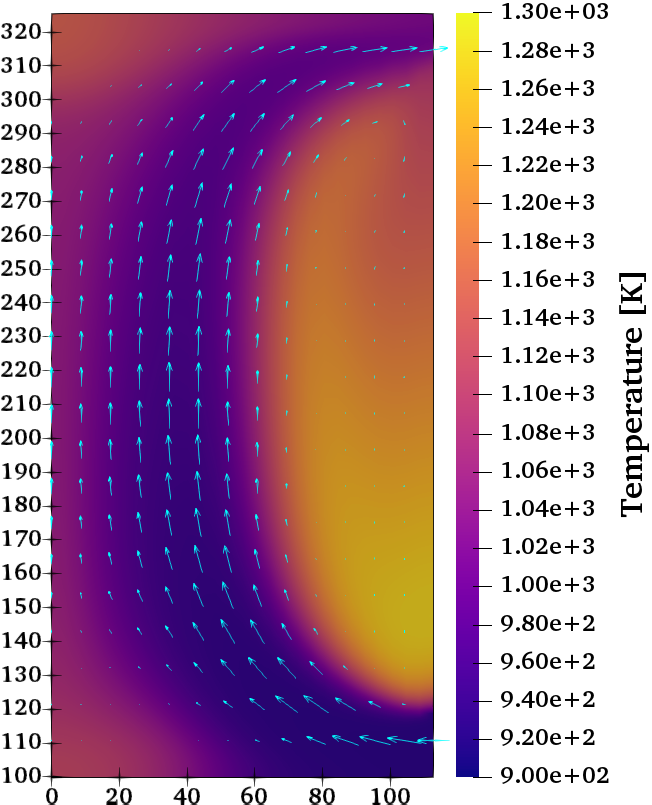
\includegraphics[width=\textwidth]{flow-temp-plasma}
    \end{subfigure}
    \hfill
    \begin{subfigure}[t]{.625\textwidth}
        \centering
        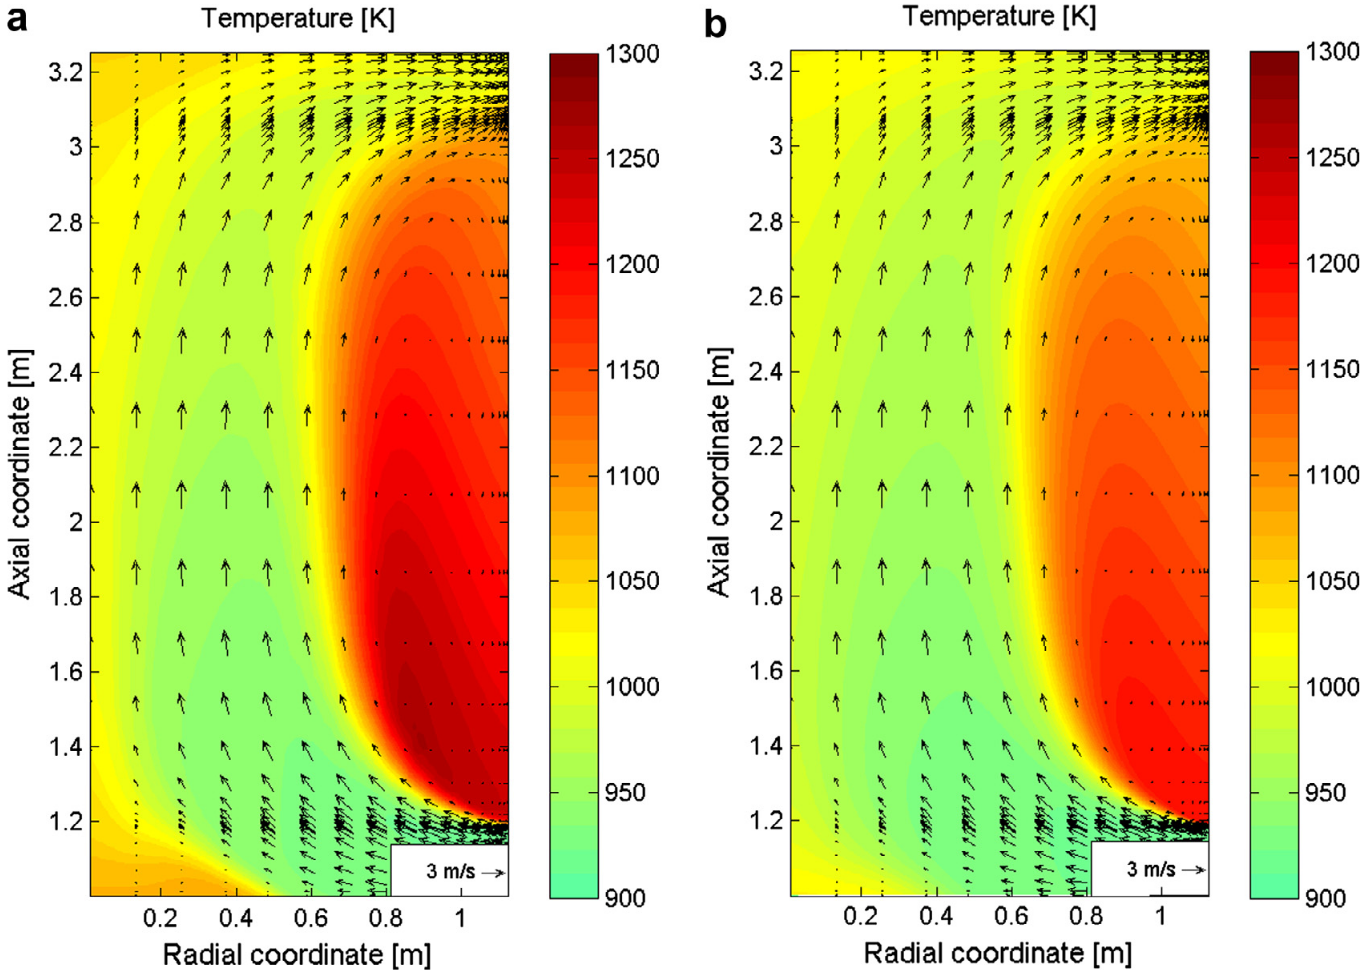
\includegraphics[width=\textwidth]{flow-temp-fiorina}
    \end{subfigure}
    \caption{Temperature and velocity fields in the core from Moltres
    (left), PoliMi (center), and TU Delft (right) models. The colors represent
    temperature according to the respective color bars and the arrows
    represent velocity fields. \cite{park_advancement_2020}}
    \label{fig:flow-temp}
\end{figure}

Figure \ref{fig:flow-temp} shows the core steady-state temperature and velocity
fields from the Moltres, PoliMi, and TU Delft models. The Moltres
model showed
good qualitative agreement with the PoliMi and TU Delft models since the plots
show similar flow and hotspot features in all three models. The salt flow
follows a parabolic path from the inlet to the outlet. A large
recirculation region formed near the right wall while the top and bottom
regions along the central axis experience relatively stagnant flow compared to
the main salt flow stream. The temperature hotspots coincide with the regions of
recirculation and stagnation because convection is the dominant heat transfer
mechanism. Maximum temperatures are observed near the bottom of the
recirculation zones; the Moltres model reports 1275 K, which is closer to the
PoliMi model ($\sim1300$ K) than the TU Delft model ($\sim1200$ K). Thus, the
incompressible flow model in Moltres performed well in reproducing the
thermal-hydraulic profiles of the \gls{MSFR} under steady-state conditions
despite the fixed turbulent viscosity assumption.

\begin{figure}[b!]
    \centering
    \begin{subfigure}[t]{.30\textwidth}
        \centering
        \vspace{.9cm}
        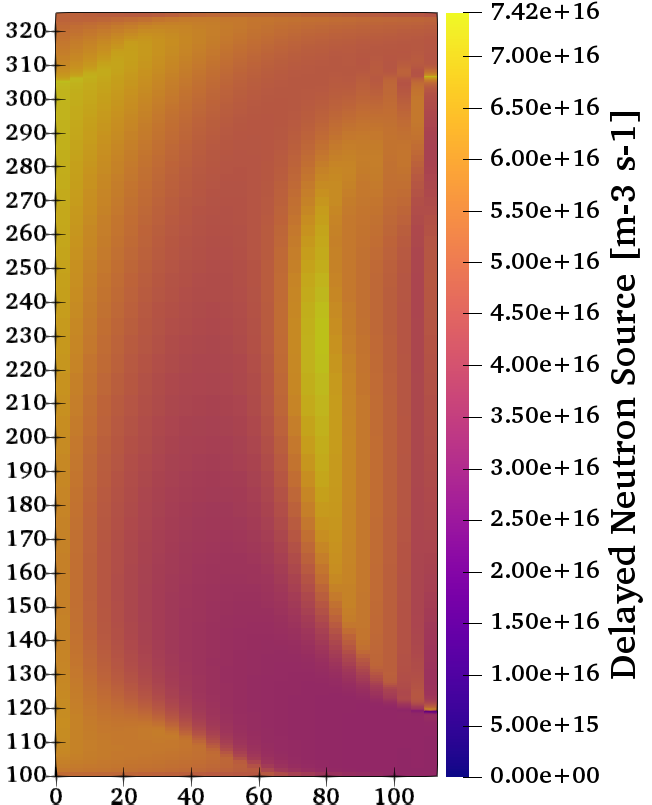
\includegraphics[width=\textwidth]{pre}
    \end{subfigure}
    \begin{subfigure}[t]{.69\textwidth}
        \centering
        \vspace{0pt}
        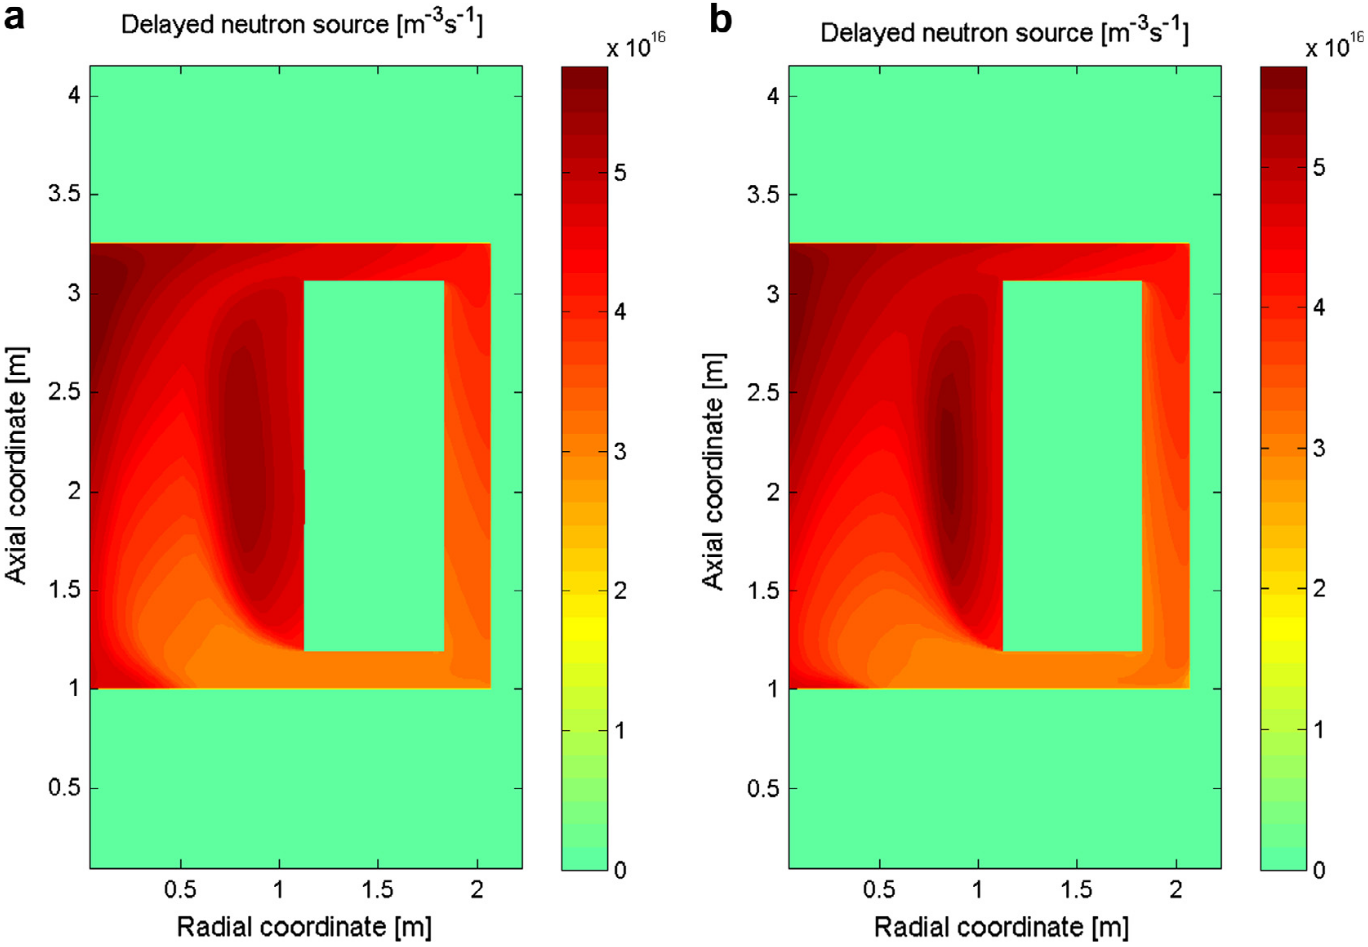
\includegraphics[width=\textwidth]{fiorina-pre}
    \end{subfigure}
    \caption{Total delayed neutron source distribution in the core from the
    Moltres (left), PoliMi (center), and TU Delft (right) models.}
    \label{fig:pre}
\end{figure}

Moltres reported a peak total neutron flux of $9.80 \times 10^{15}$
cm$^{-2}\cdot$s$^{-1}$, which is close to the 8.6 and 9.0 $\times 10^{15}$
cm$^{-2}\cdot$s$^{-1}$ values reported by Fiorina et al.
\cite{fiorina_molten_2013} and \cite{aufiero_development_2014}. However, the
delayed neutron source distribution from the Moltres model exhibits some
differences compared to the PoliMi and TU Delft models, as shown in Figure
\ref{fig:pre}. The Moltres model retains fewer precursors than the other two
models, resulting in a higher 44.16\% out-of-core delayed neutron emissions
compared with the 34.80\% and 34.85\% from the other models
\cite{park_advancement_2020}. Therefore, the incompressible flow model with
constant turbulent viscosity fell short of accurately capturing precursor
drift in the \gls{MSFR}.

\begin{figure}[htb]
    \centering
    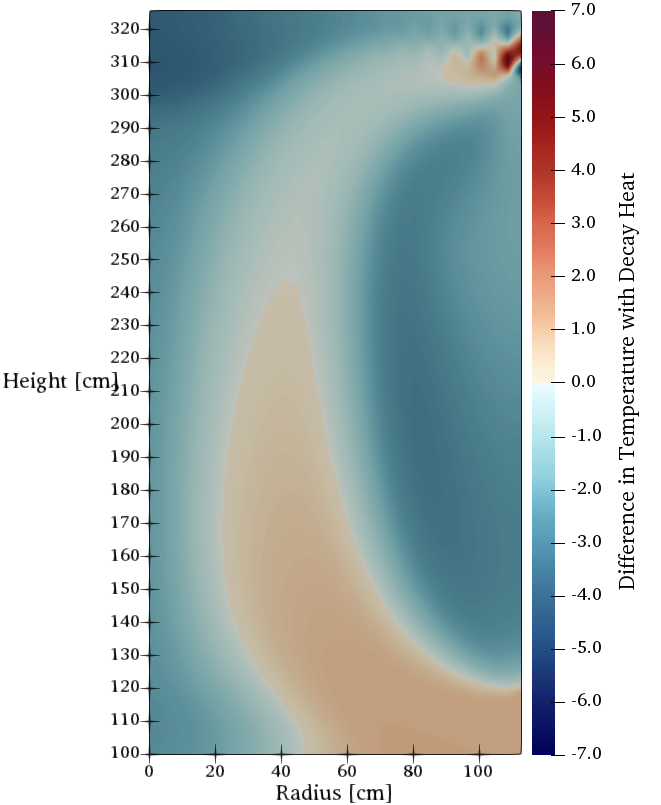
\includegraphics[width=.5\textwidth]{decay-heat-temp}
    \caption{Difference in core temperatures at steady-state with decay heat
    relative to the result without decay heat (Figure \ref{fig:flow-temp}).}
    \label{fig:decayheattemp}
\end{figure}

This work also compared steady-state temperature distributions with and without
the decay heat model. As expected, the decay heat model effectively flattens
the heat source distribution, reducing the maximum
temperatures and increasing the minimum temperatures observed in the model.
Figure \ref{fig:decayheattemp} shows a decrease in temperature in the hotspot
regions and an increase in temperature near the inlet, the coolest
region in the core.

For the transient studies, this work considered unprotected reactivity
insertion, loss-of-heat-sink, loss-of-flow, and pump-overspeed accidents. The
term ``unprotected'' signifies accident scenarios without reactor SCRAM.
Moltres reproduced similar trends observed in the PoliMi and TU Delft
models for the reactivity insertion and loss-of-heat-sink scenarios. For
instance, Figure \ref{fig:200pcmheat} shows the power output response of the
three models following a 200 pcm step reactivity insertion. The lower peak from
the Moltres model is attributed to the stronger negative fuel temperature
reactivity feedback coefficient of $-7.184$ pcm$\cdot$K$^{-1}$ compared to
approximately $-6.5$ pcm$\cdot$K$^{-1}$ for the PoliMi and TU Delft models.

\begin{figure}[htb!]
    \centering
    \begin{minipage}[b]{.49\textwidth}
      \centering
      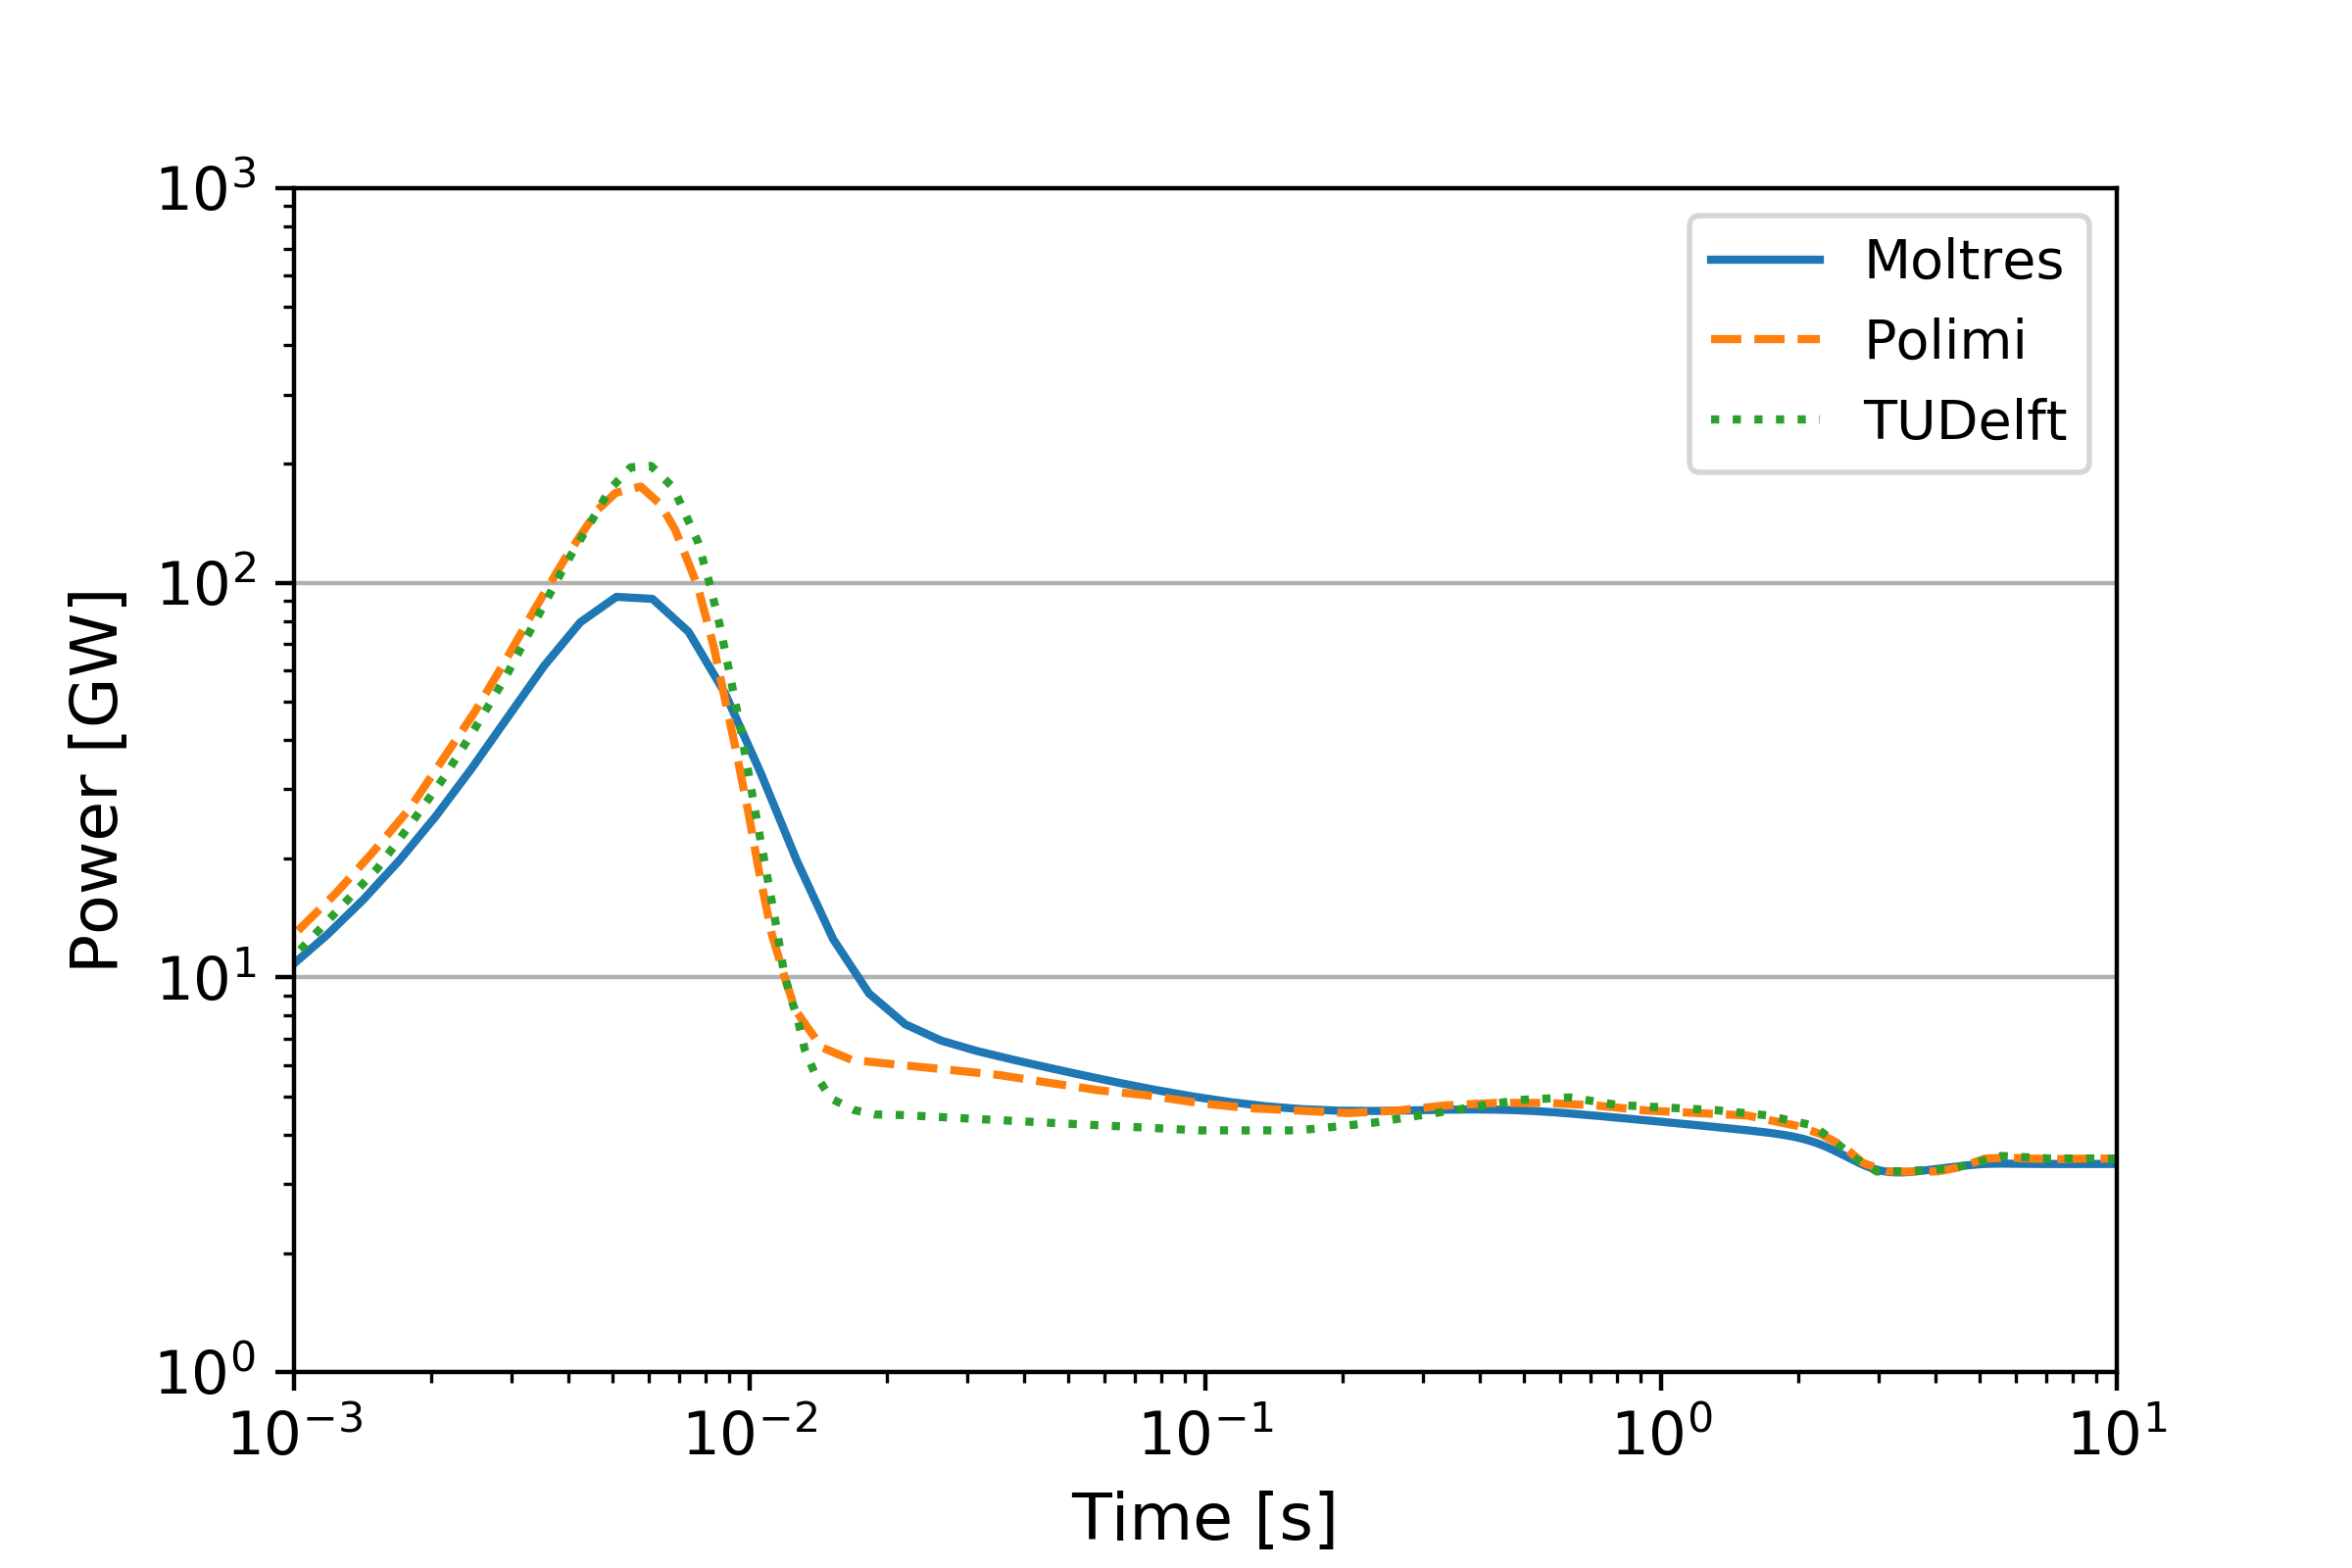
\includegraphics[width=\textwidth]{200pcm-heat}
      \caption{Power output following a 200 pcm step-wise unprotected reactivity
        insertion in the Moltres, PoliMi, and
        TU Delft models \cite{fiorina_modelling_2014}.}
      \label{fig:200pcmheat}
    \end{minipage}
    \hfill
    \begin{minipage}[b]{.49\textwidth}
      \centering
      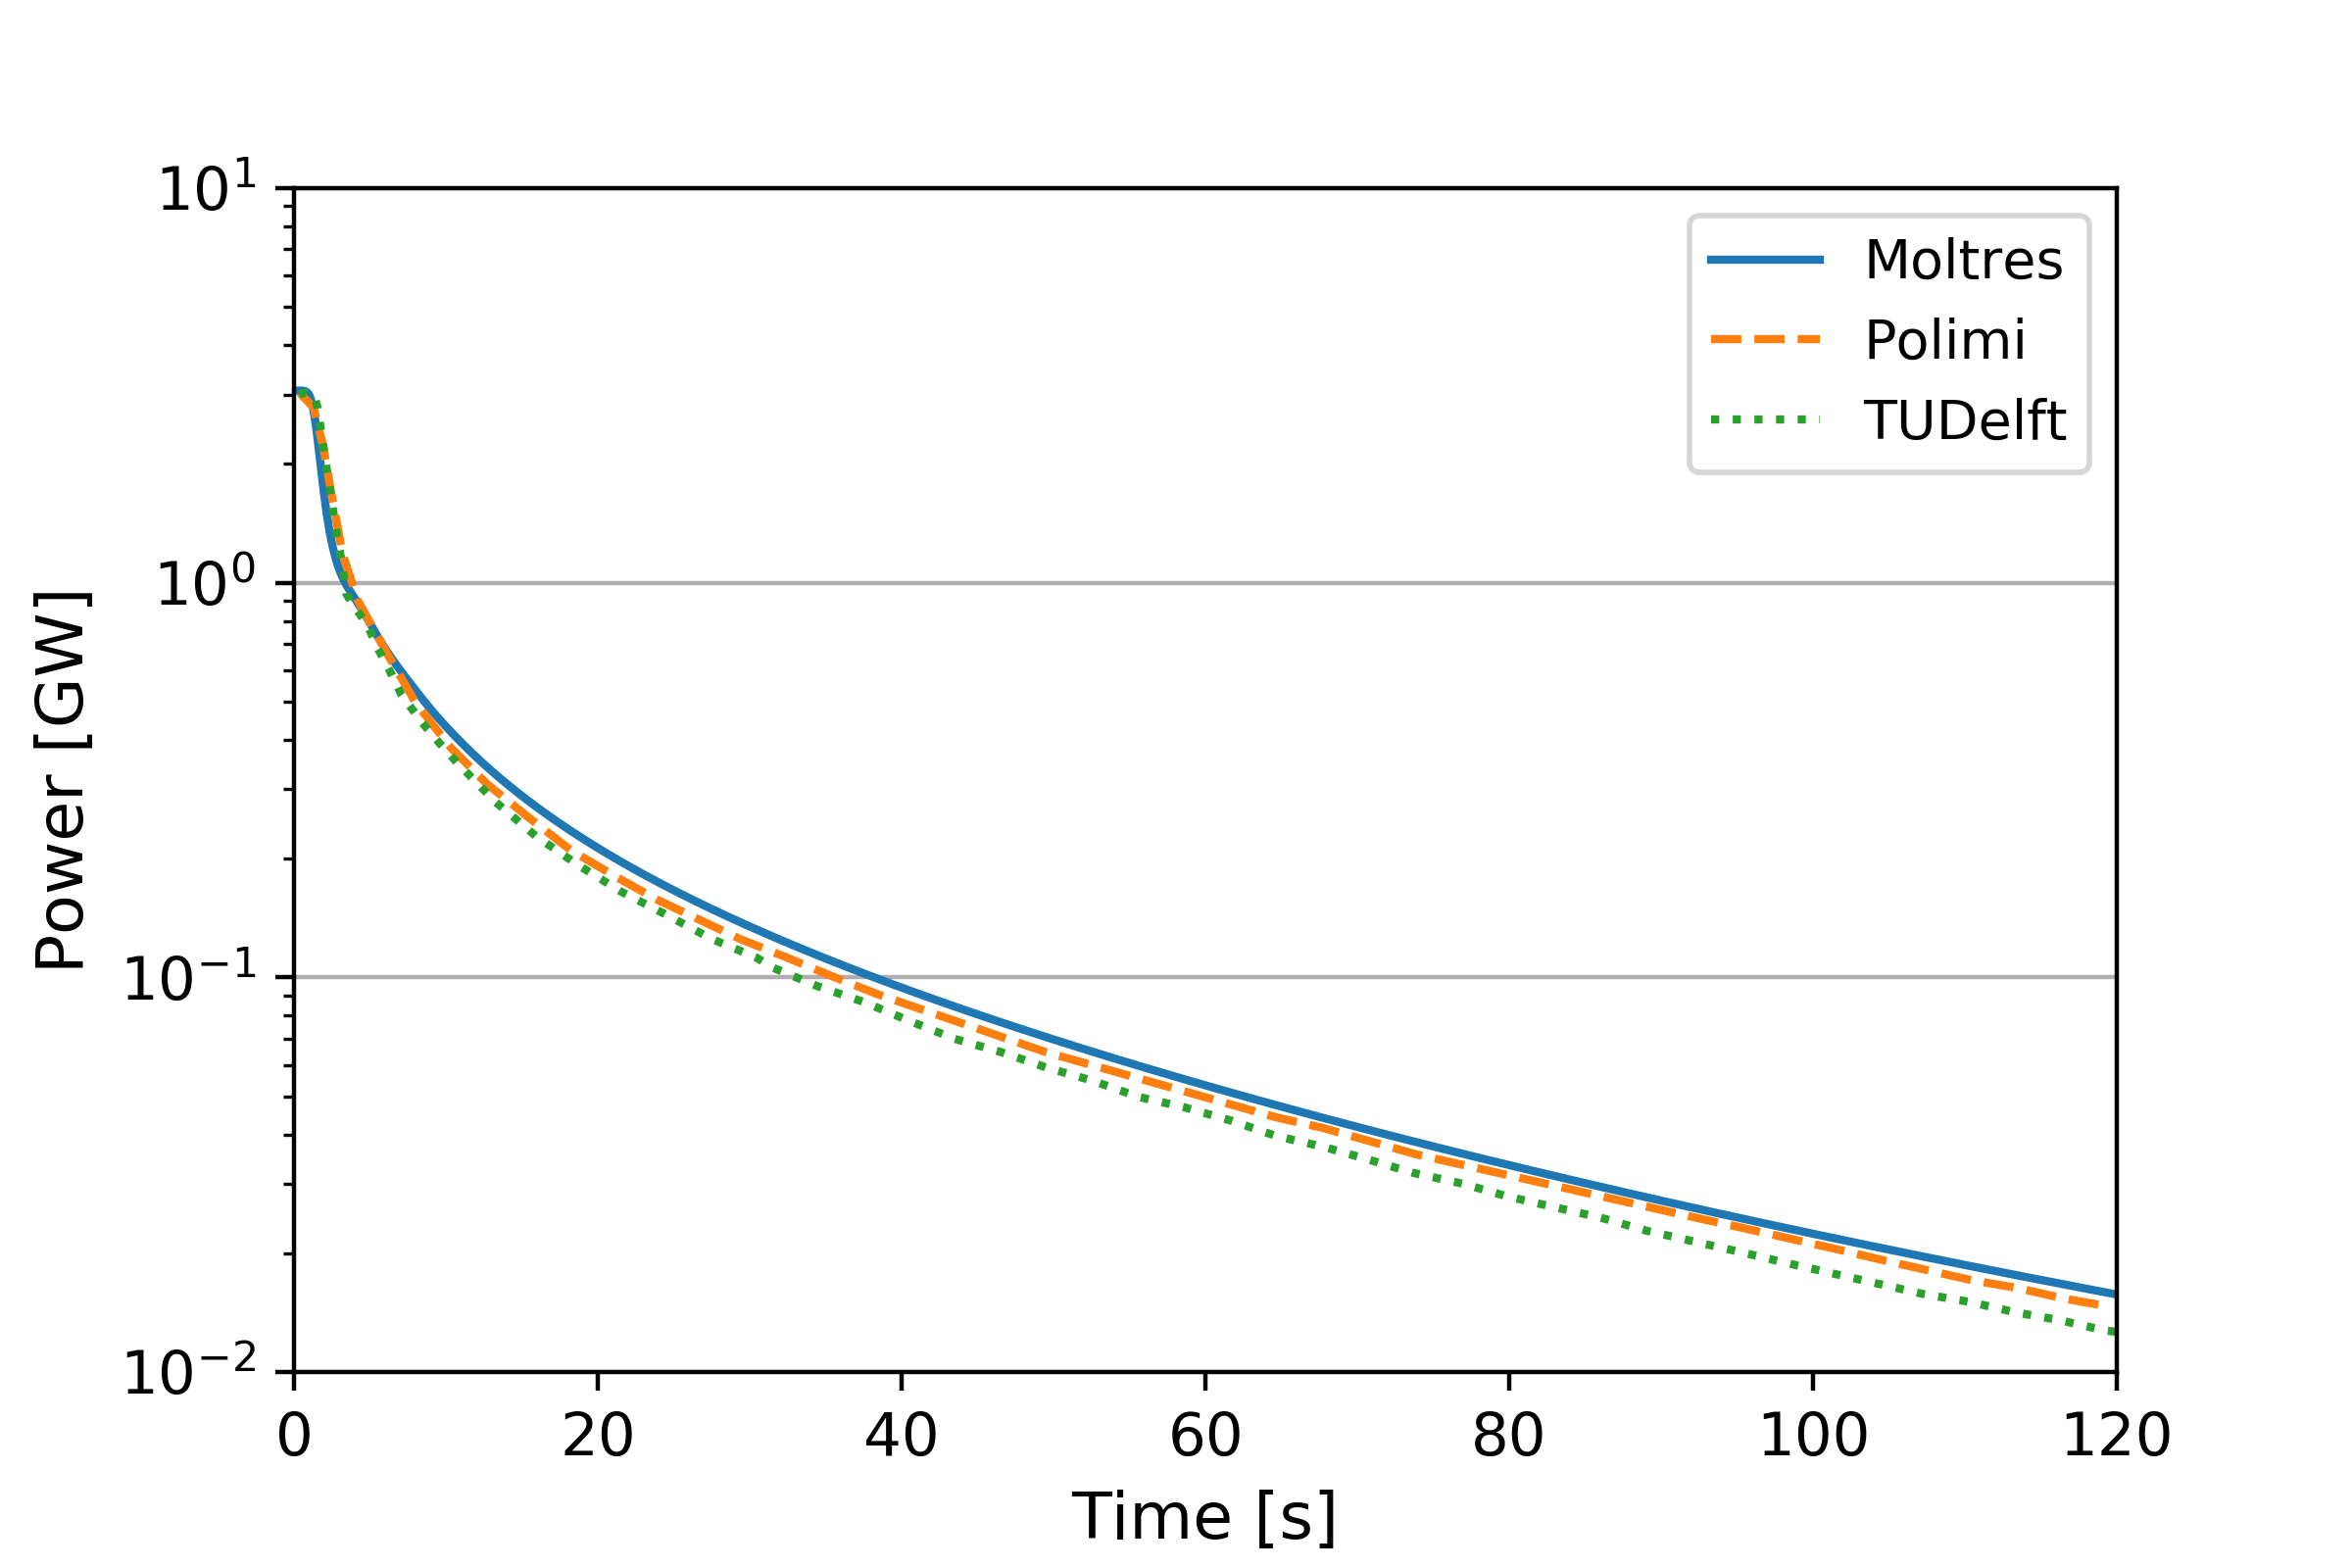
\includegraphics[width=\textwidth]{lohs-heat}
      \caption{Power output during
        an unprotected loss of heat sink transient in the Moltres, PoliMi, and
        TU Delft models \cite{fiorina_modelling_2014} without decay heat.}
      \label{fig:lohsheat}
    \end{minipage}
\end{figure}

The loss-of-heat-sink transients were performed with and without the decay heat
model because the TU Delft model did not possess this capability. As shown in
Figure \ref{fig:lohsheat}, without decay heat, all three models reported
similar power output responses following the loss of cooling through the heat
exchanger modeled as an exponential decrease in heat removal rate with a time
constant of 1 s. As prompt heat generation decreases due to rising core
temperatures and the negative temperature reactivity feedback, decay heat
becomes a significant heat source. We observe this in Figure
\ref{fig:moltresdecaypower}, which shows decay heat output overtaking prompt
heat output 34 s into the accident scenario. With the decay heat model, the
Moltres model shows good agreement with the PoliMi model. The temperature
increase averaged over the fuel salt loop falls within 10\% of the PoliMi
model (Figure \ref{fig:polimidecaytemp}).

\begin{figure}[htb!]
	\centering
	\begin{minipage}[t]{0.485\columnwidth}
	    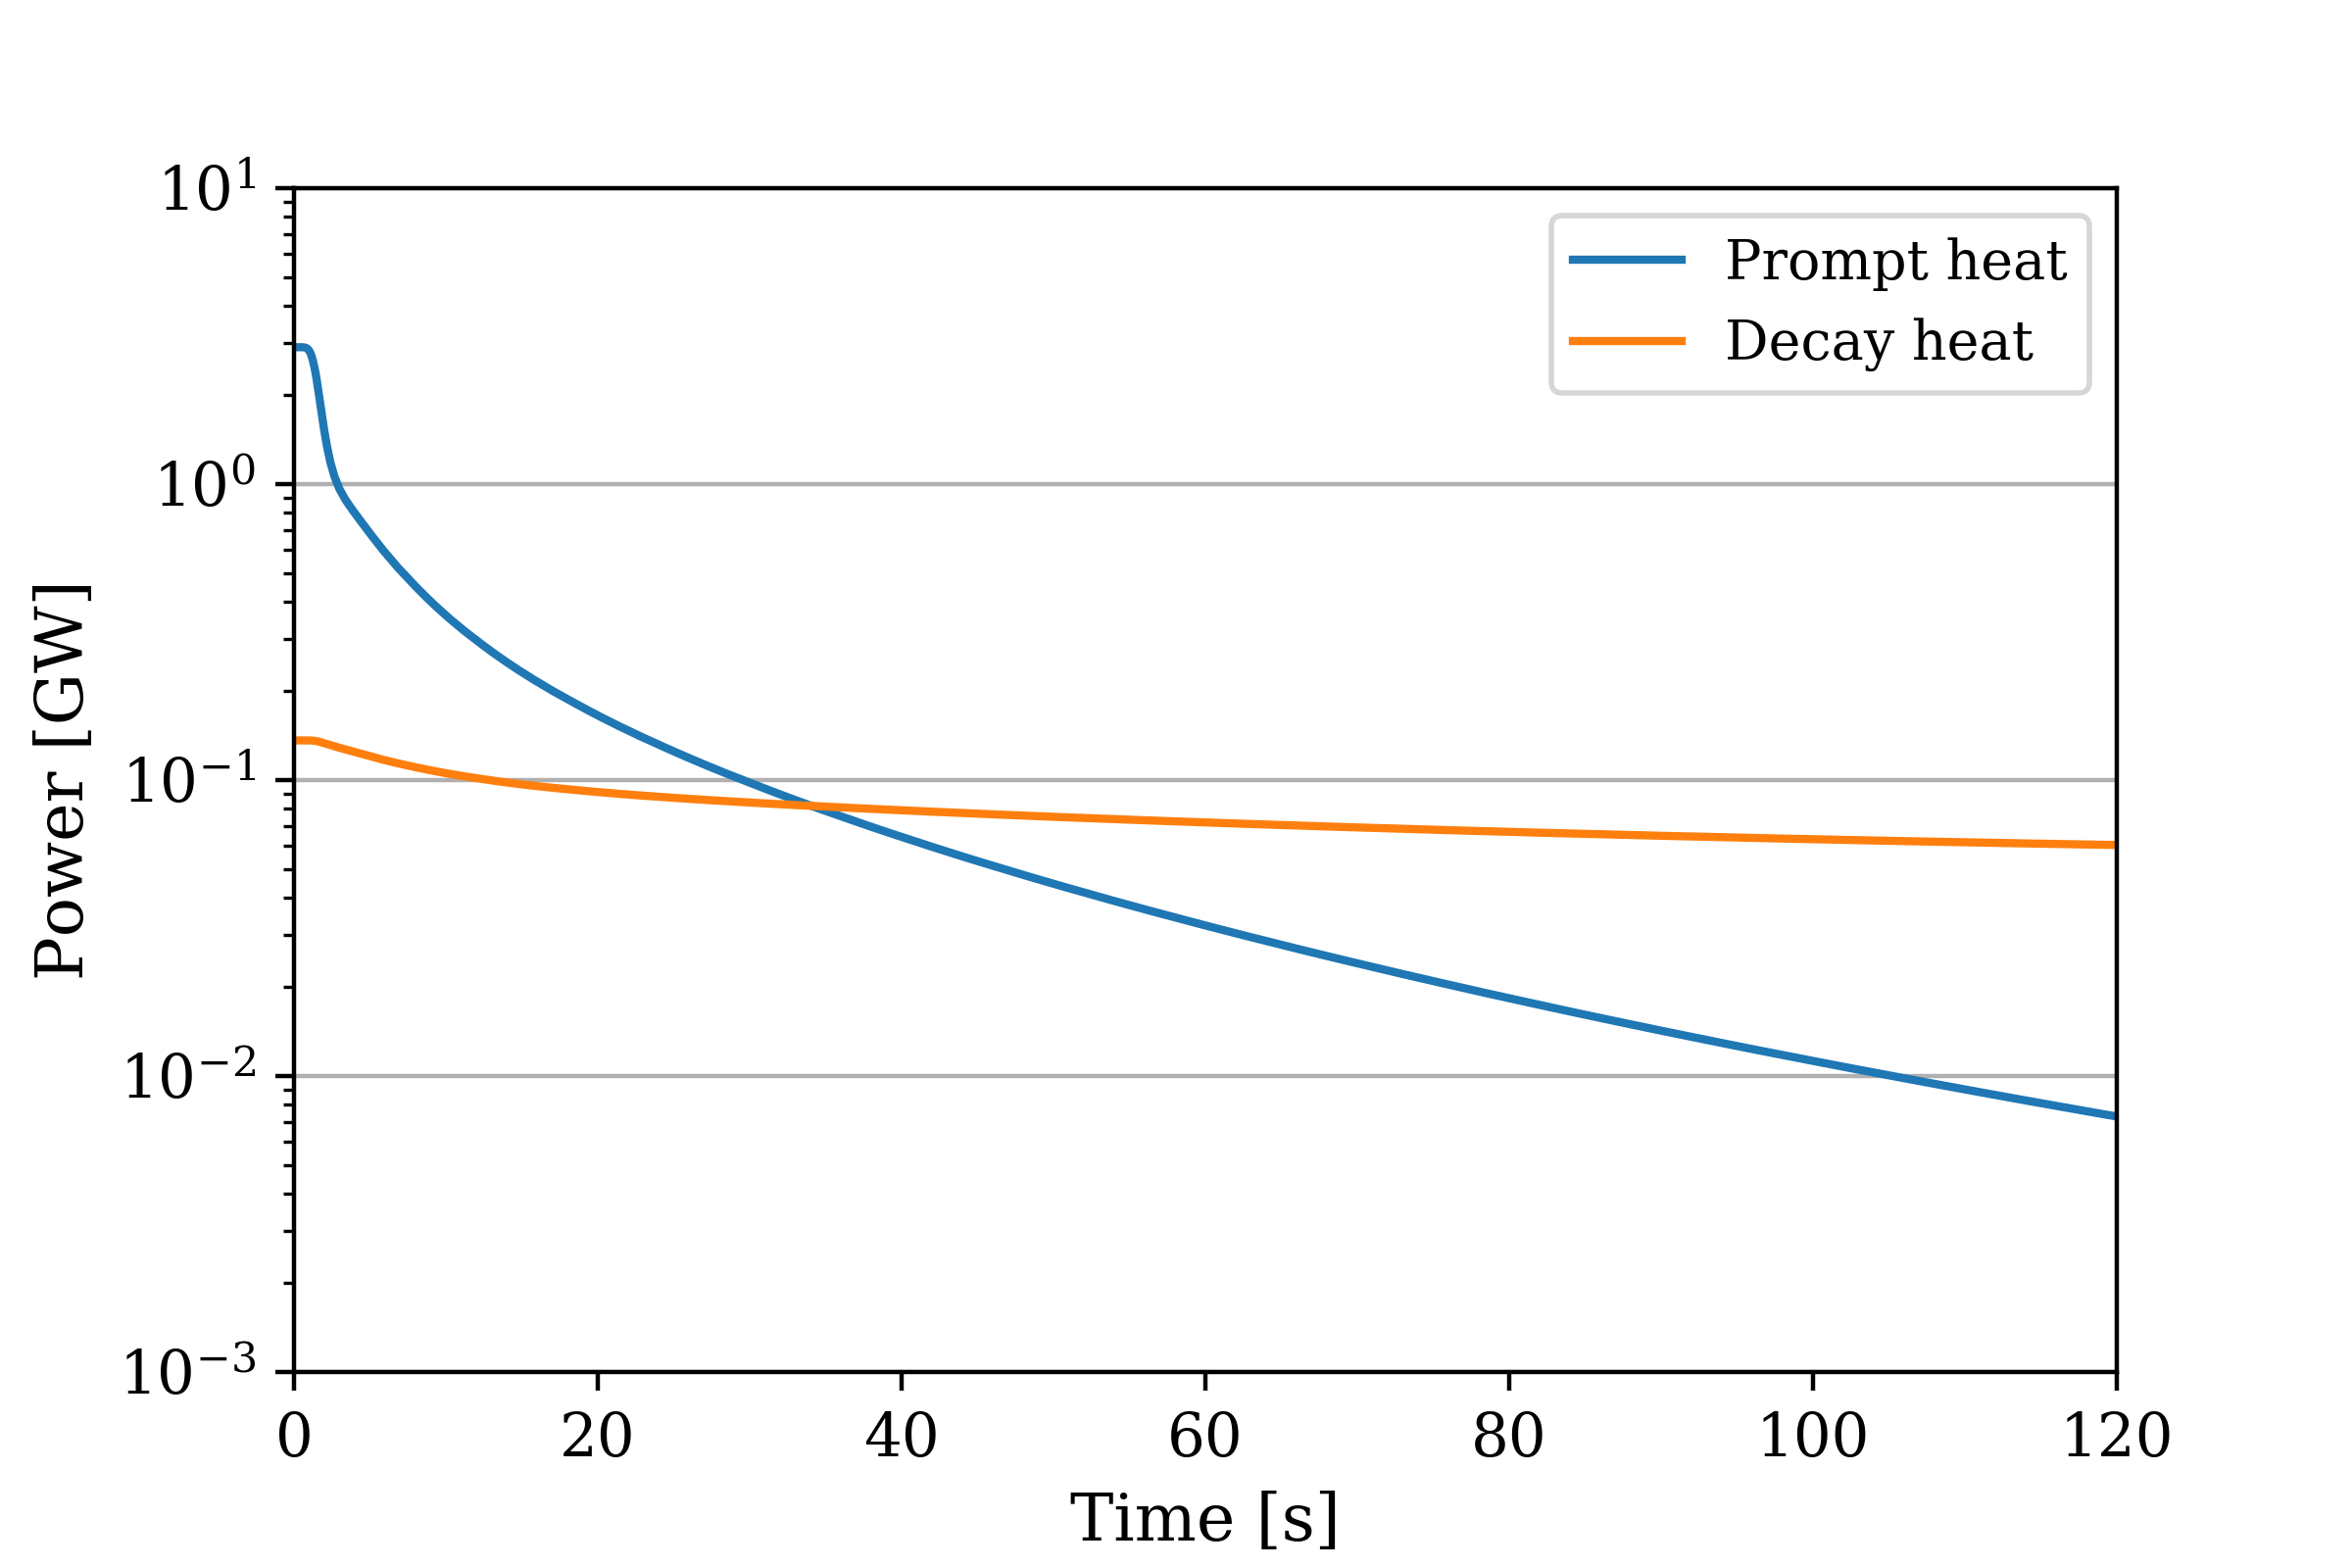
\includegraphics[width=\columnwidth]{moltres-decay-power}
	    \caption{Power output during
    an unprotected loss of heat sink transient in the Moltres model with
    decay heat.}
	    \label{fig:moltresdecaypower}
	\end{minipage}
	\hfill
	\begin{minipage}[t]{0.485\columnwidth}
	    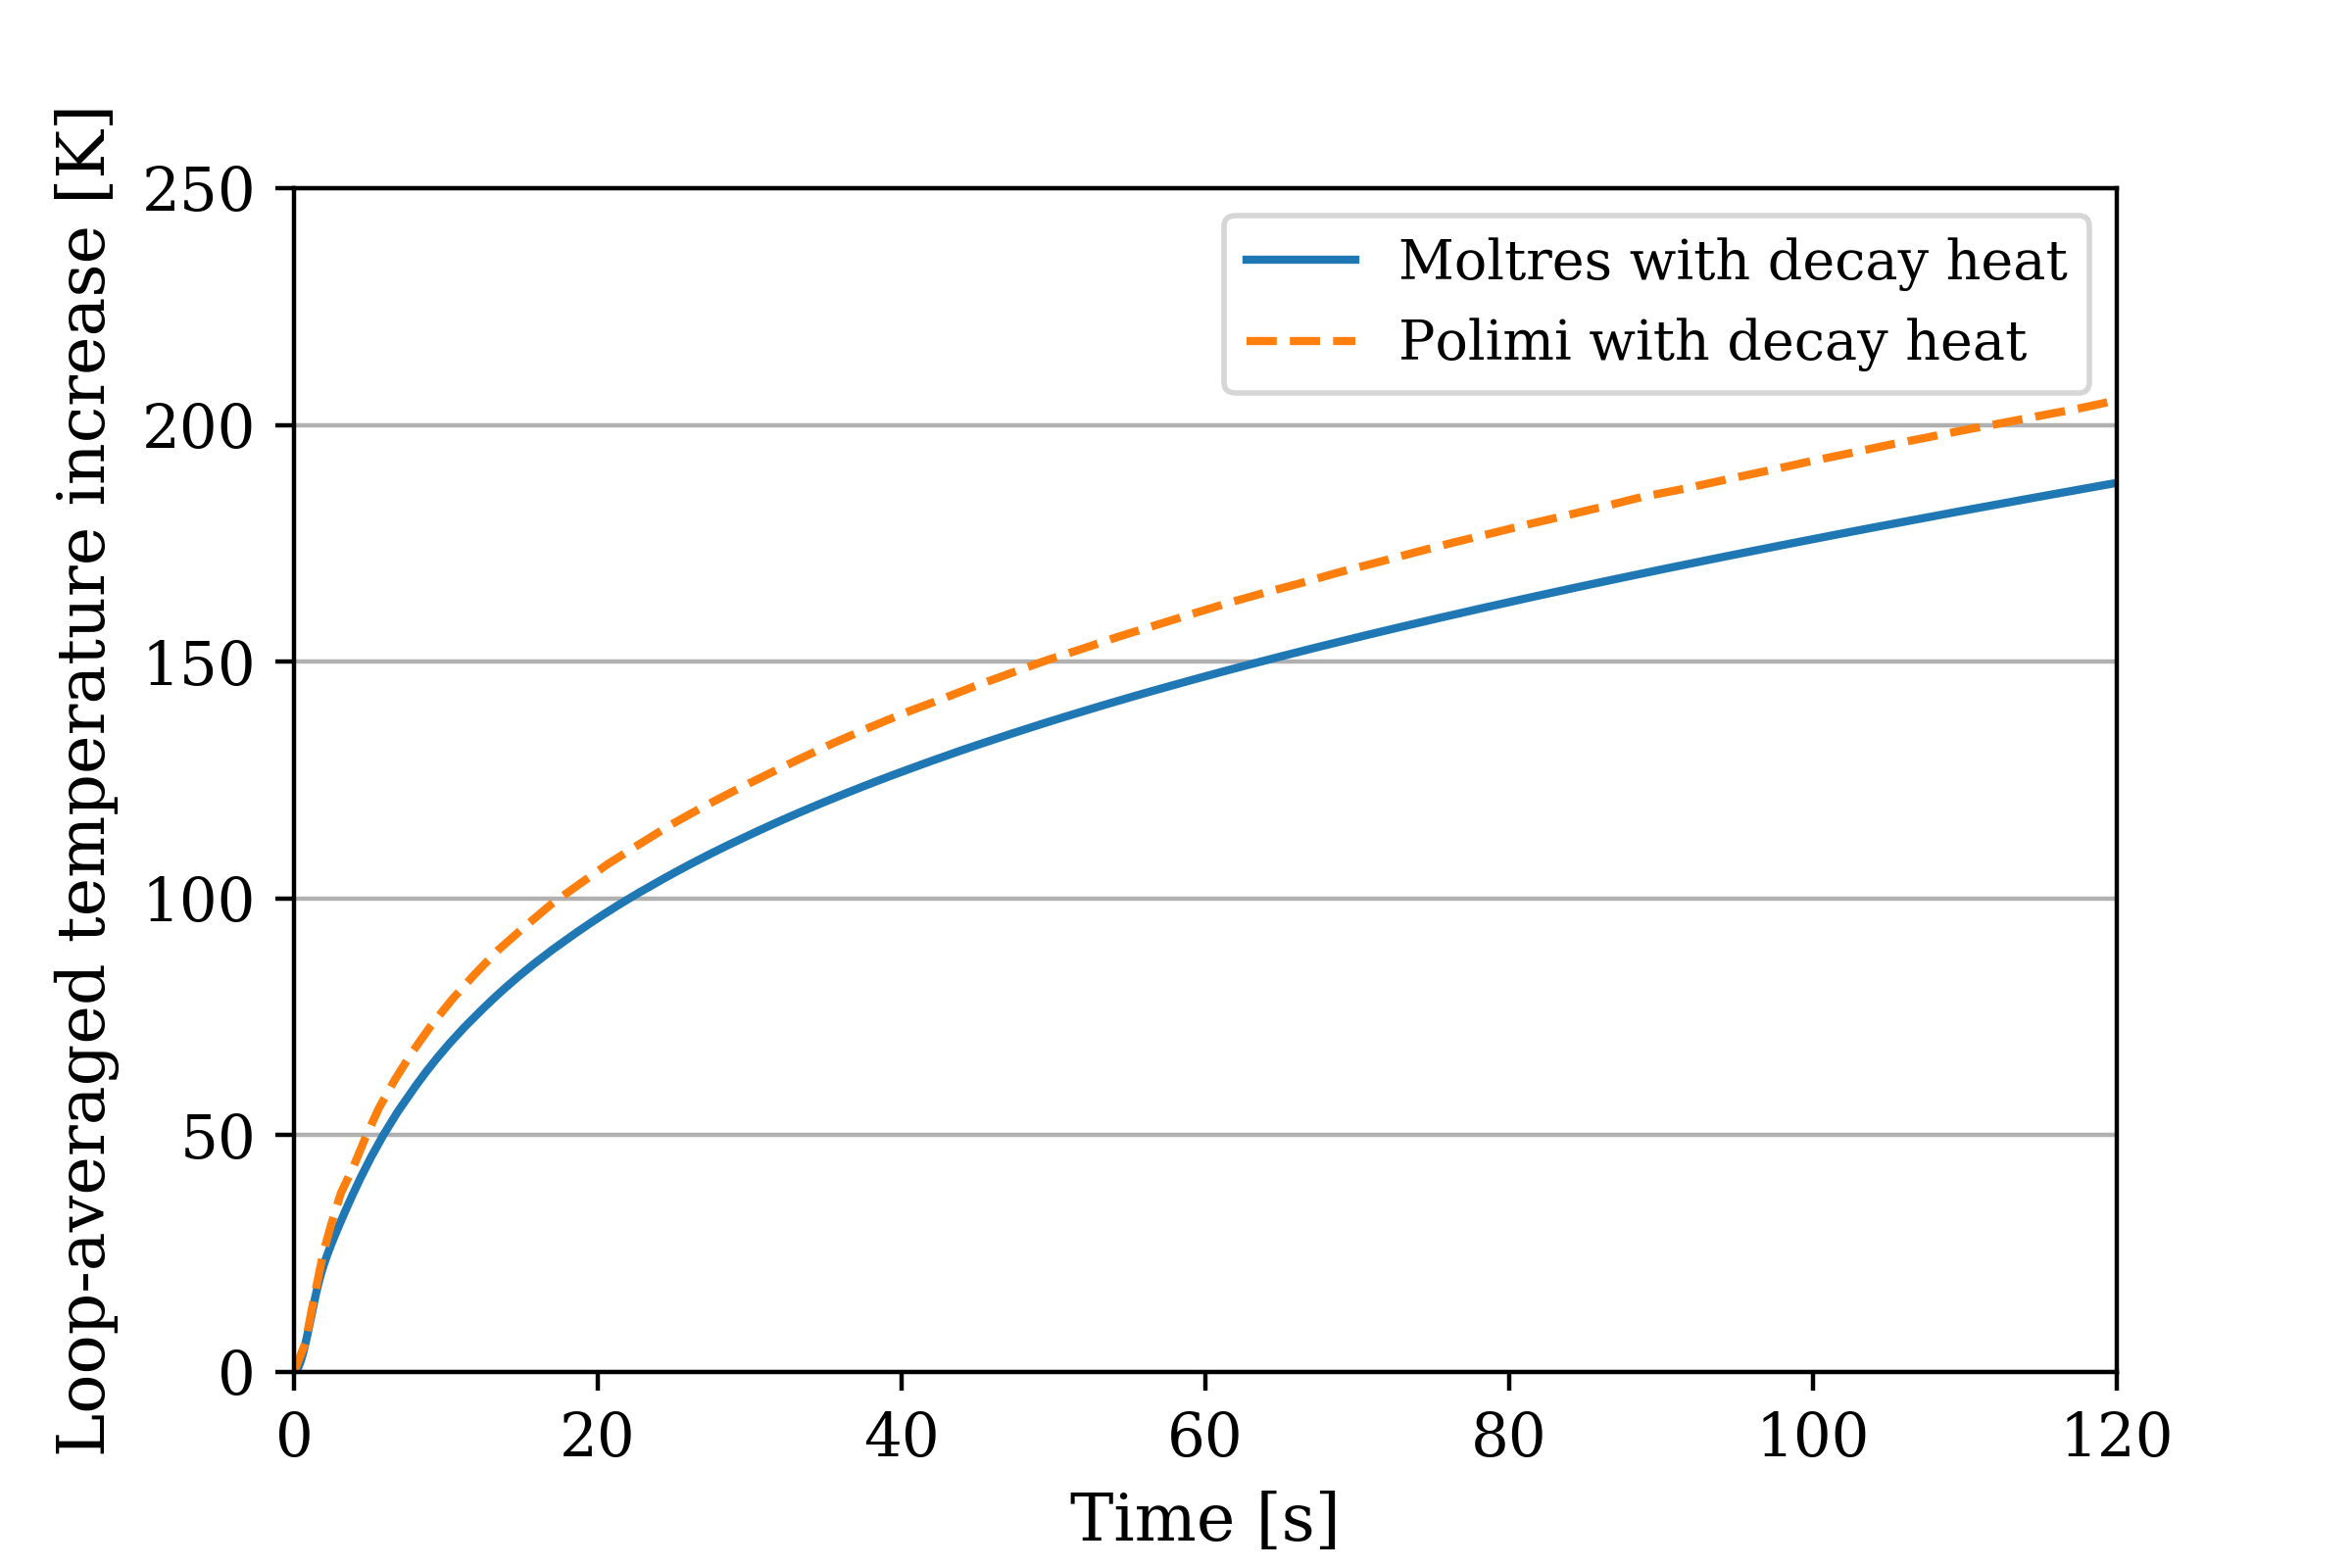
\includegraphics[width=\columnwidth]{decay-temp}
	    \caption{Loop-averaged temperature increase during
    an unprotected loss of heat sink transient in the Moltres and PoliMi
    models \cite{fiorina_modelling_2014} with decay heat.}
	    \label{fig:polimidecaytemp}
	\end{minipage}
\end{figure}

On the other hand, for the pump-initiated accident scenarios, significant
changes in the flow affected the validity of the uniform turbulent viscosity
assumption. These transients required ad hoc adjustments to the uniform
turbulent viscosity assumption as a function of volumetric flow to reproduce
the trends observed in the PoliMi and TU Delft models. Furthermore, unlike the
other two models, the Moltres model did not apply the Boussinesq approximation
for buoyancy-driven flow. The Moltres model could replicate expected trends in
the pump overspeed scenario (Figure \ref{fig:poshort}), but performed
poorly in the loss of flow scenario (Figure \ref{fig:lof}). In the latter
scenario, buoyancy effects become significant as the model loses forced flow.

\begin{figure}[htb!]
    \centering
    \begin{subfigure}[t]{.485\textwidth}
        \centering
        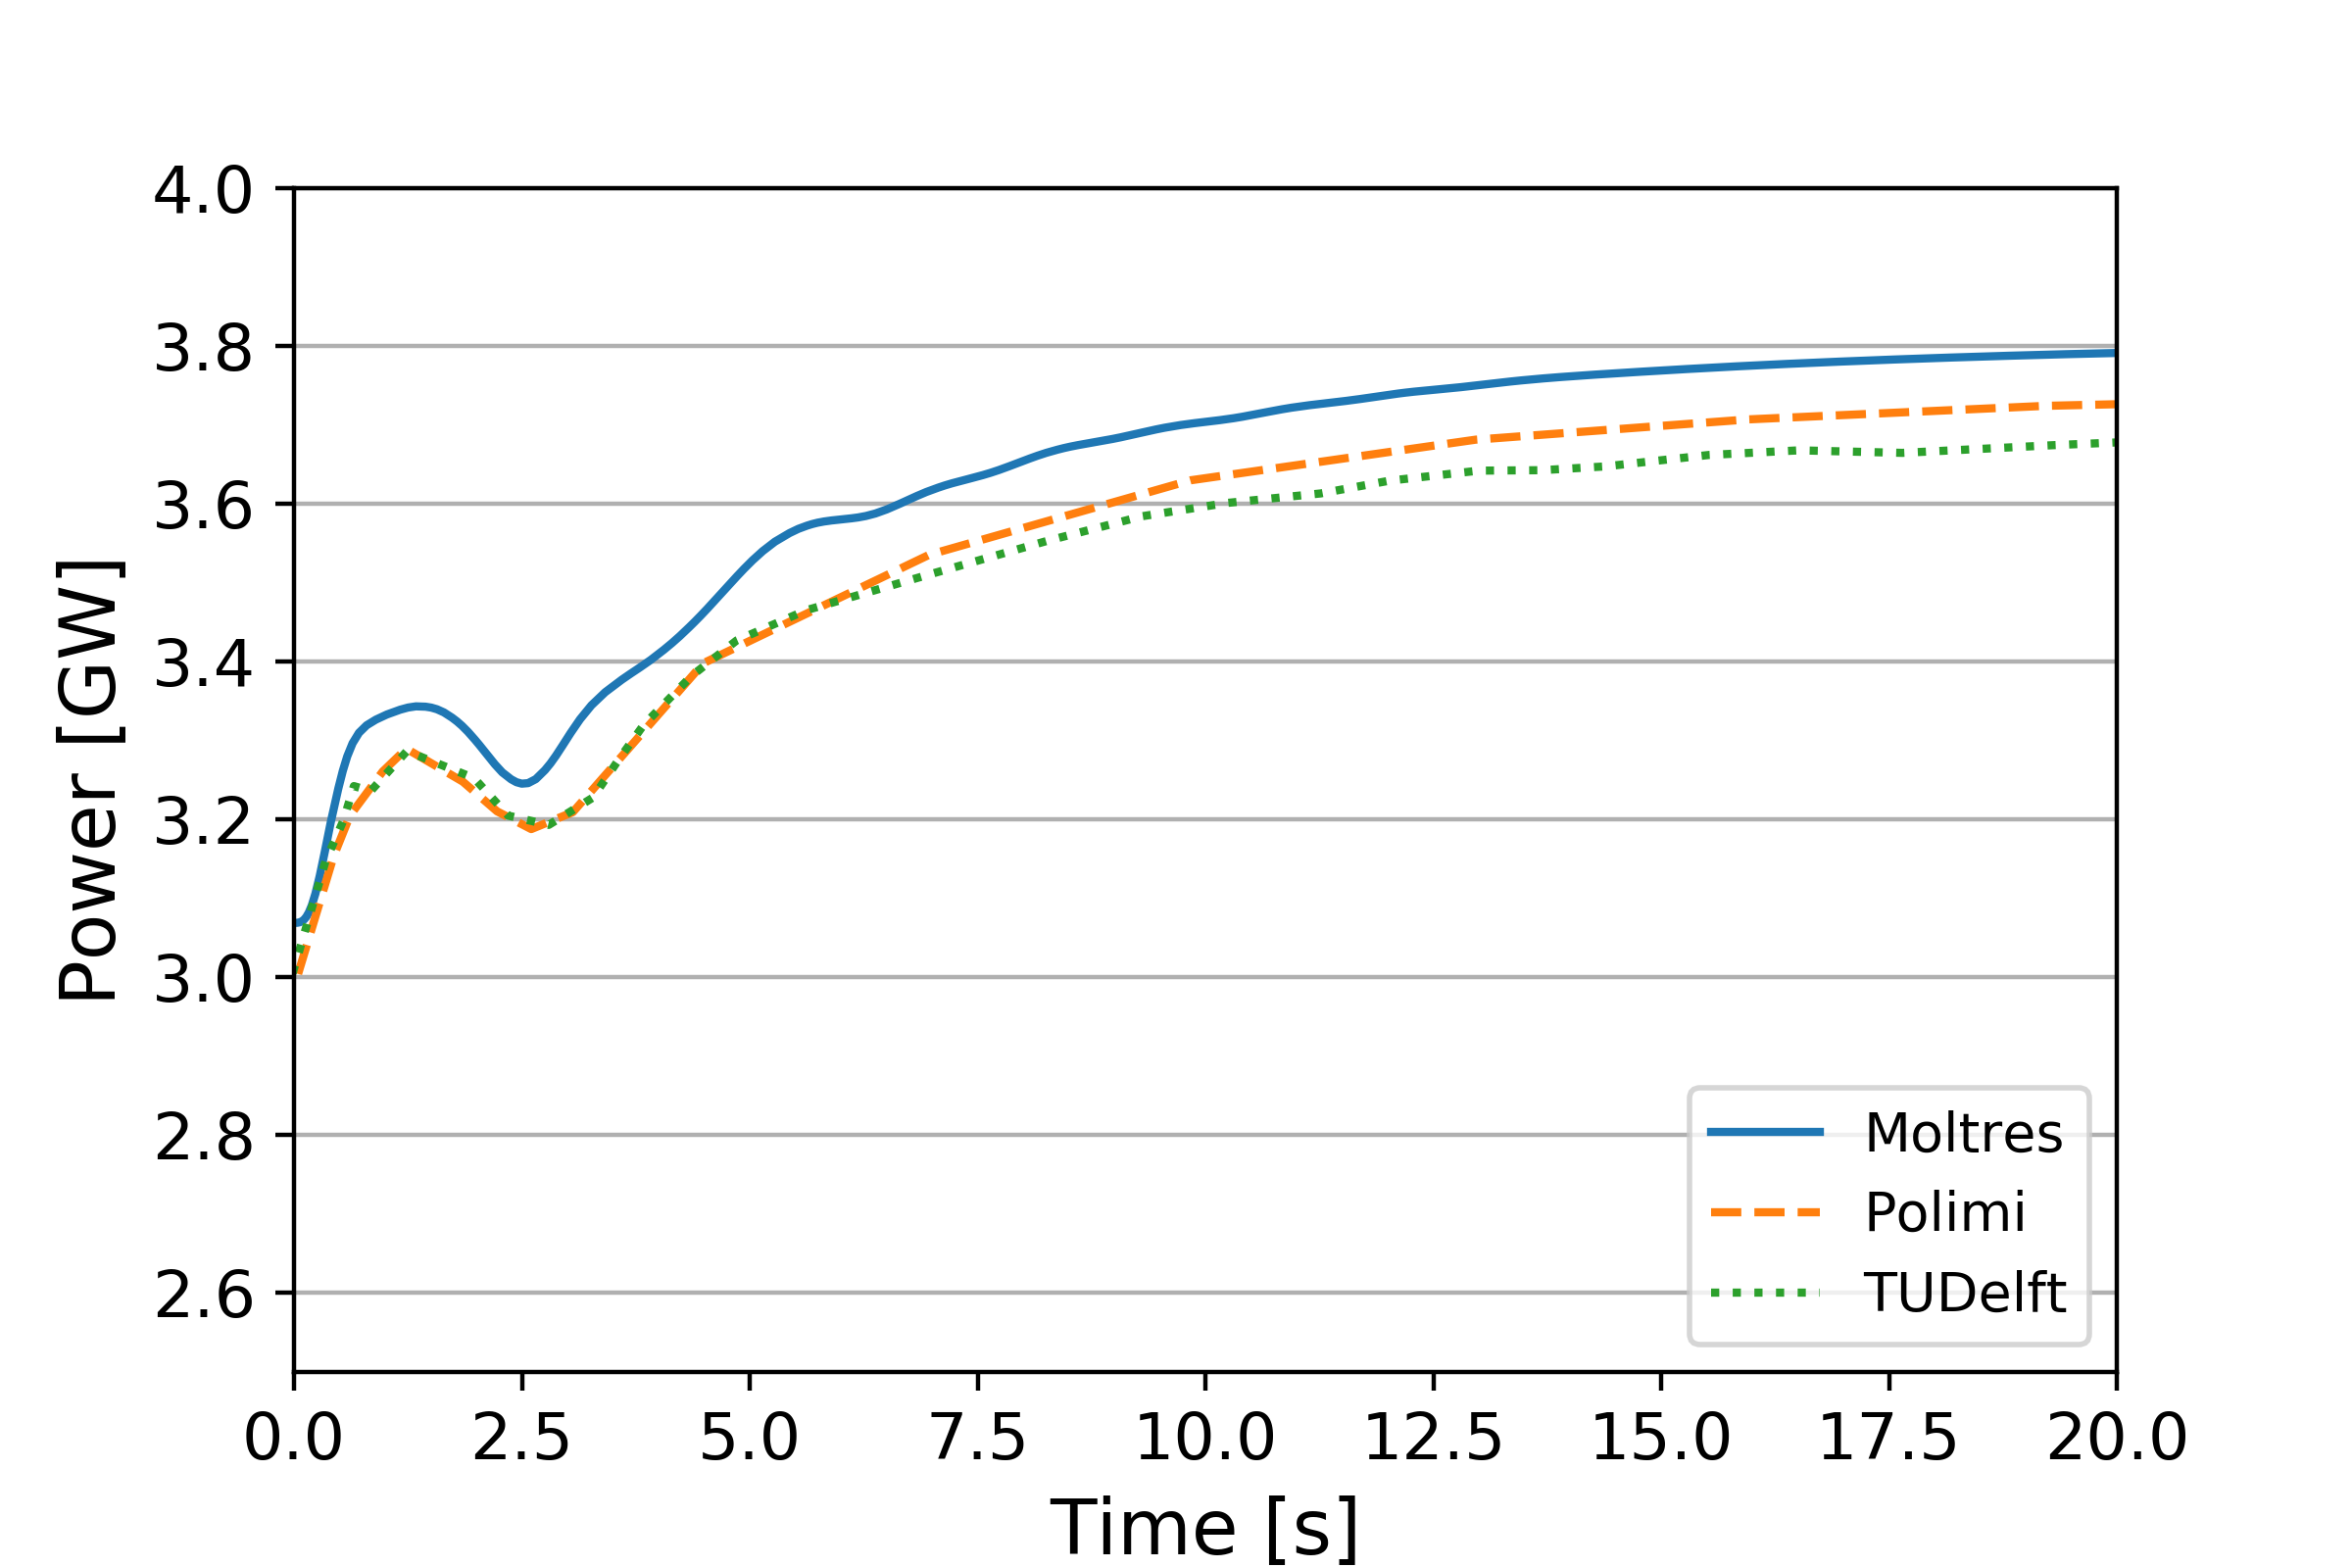
\includegraphics[width=\textwidth]{po-heat-short}
    \end{subfigure}
    \hfill
    \begin{subfigure}[t]{.485\textwidth}
        \centering
        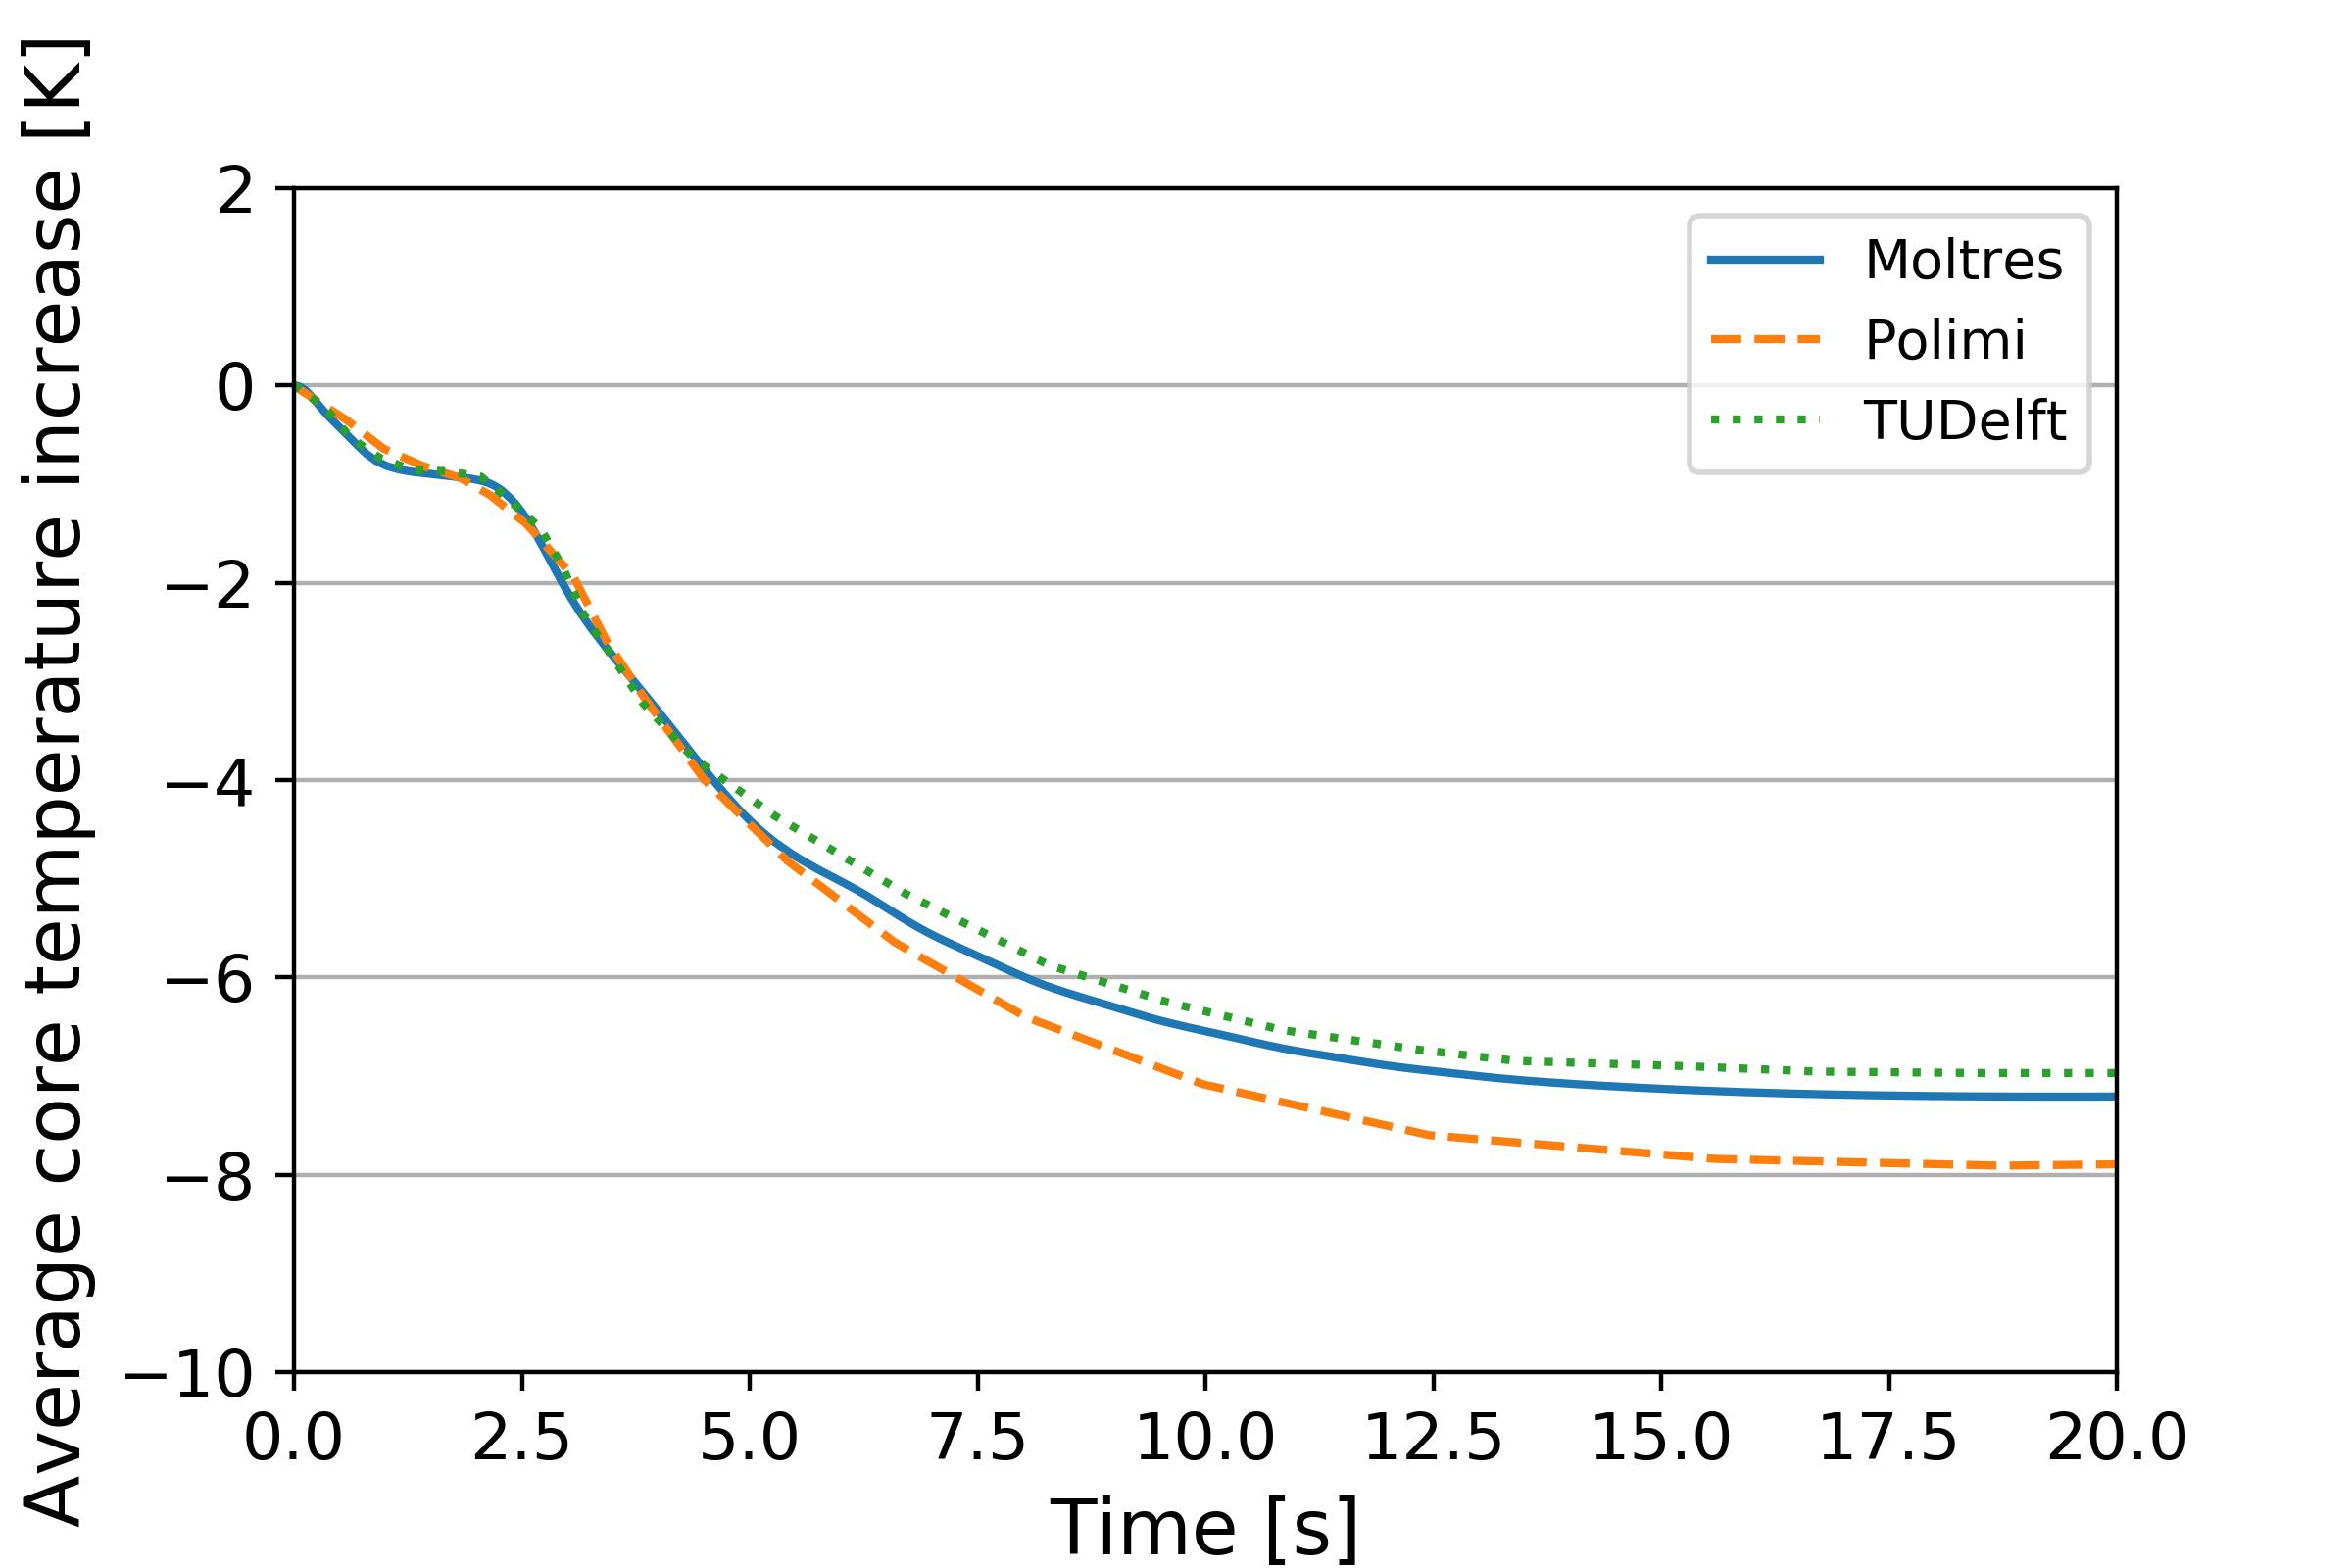
\includegraphics[width=\textwidth]{po-temp-short}
    \end{subfigure}
    \caption{Average core temperature increase during
    an unprotected pump overspeed transient in the Moltres, PoliMi, and
    TU Delft models \cite{fiorina_modelling_2014}.}
    \label{fig:poshort}
\end{figure}

\begin{figure}[htb!]
    \centering
    \begin{subfigure}[t]{.485\textwidth}
        \centering
        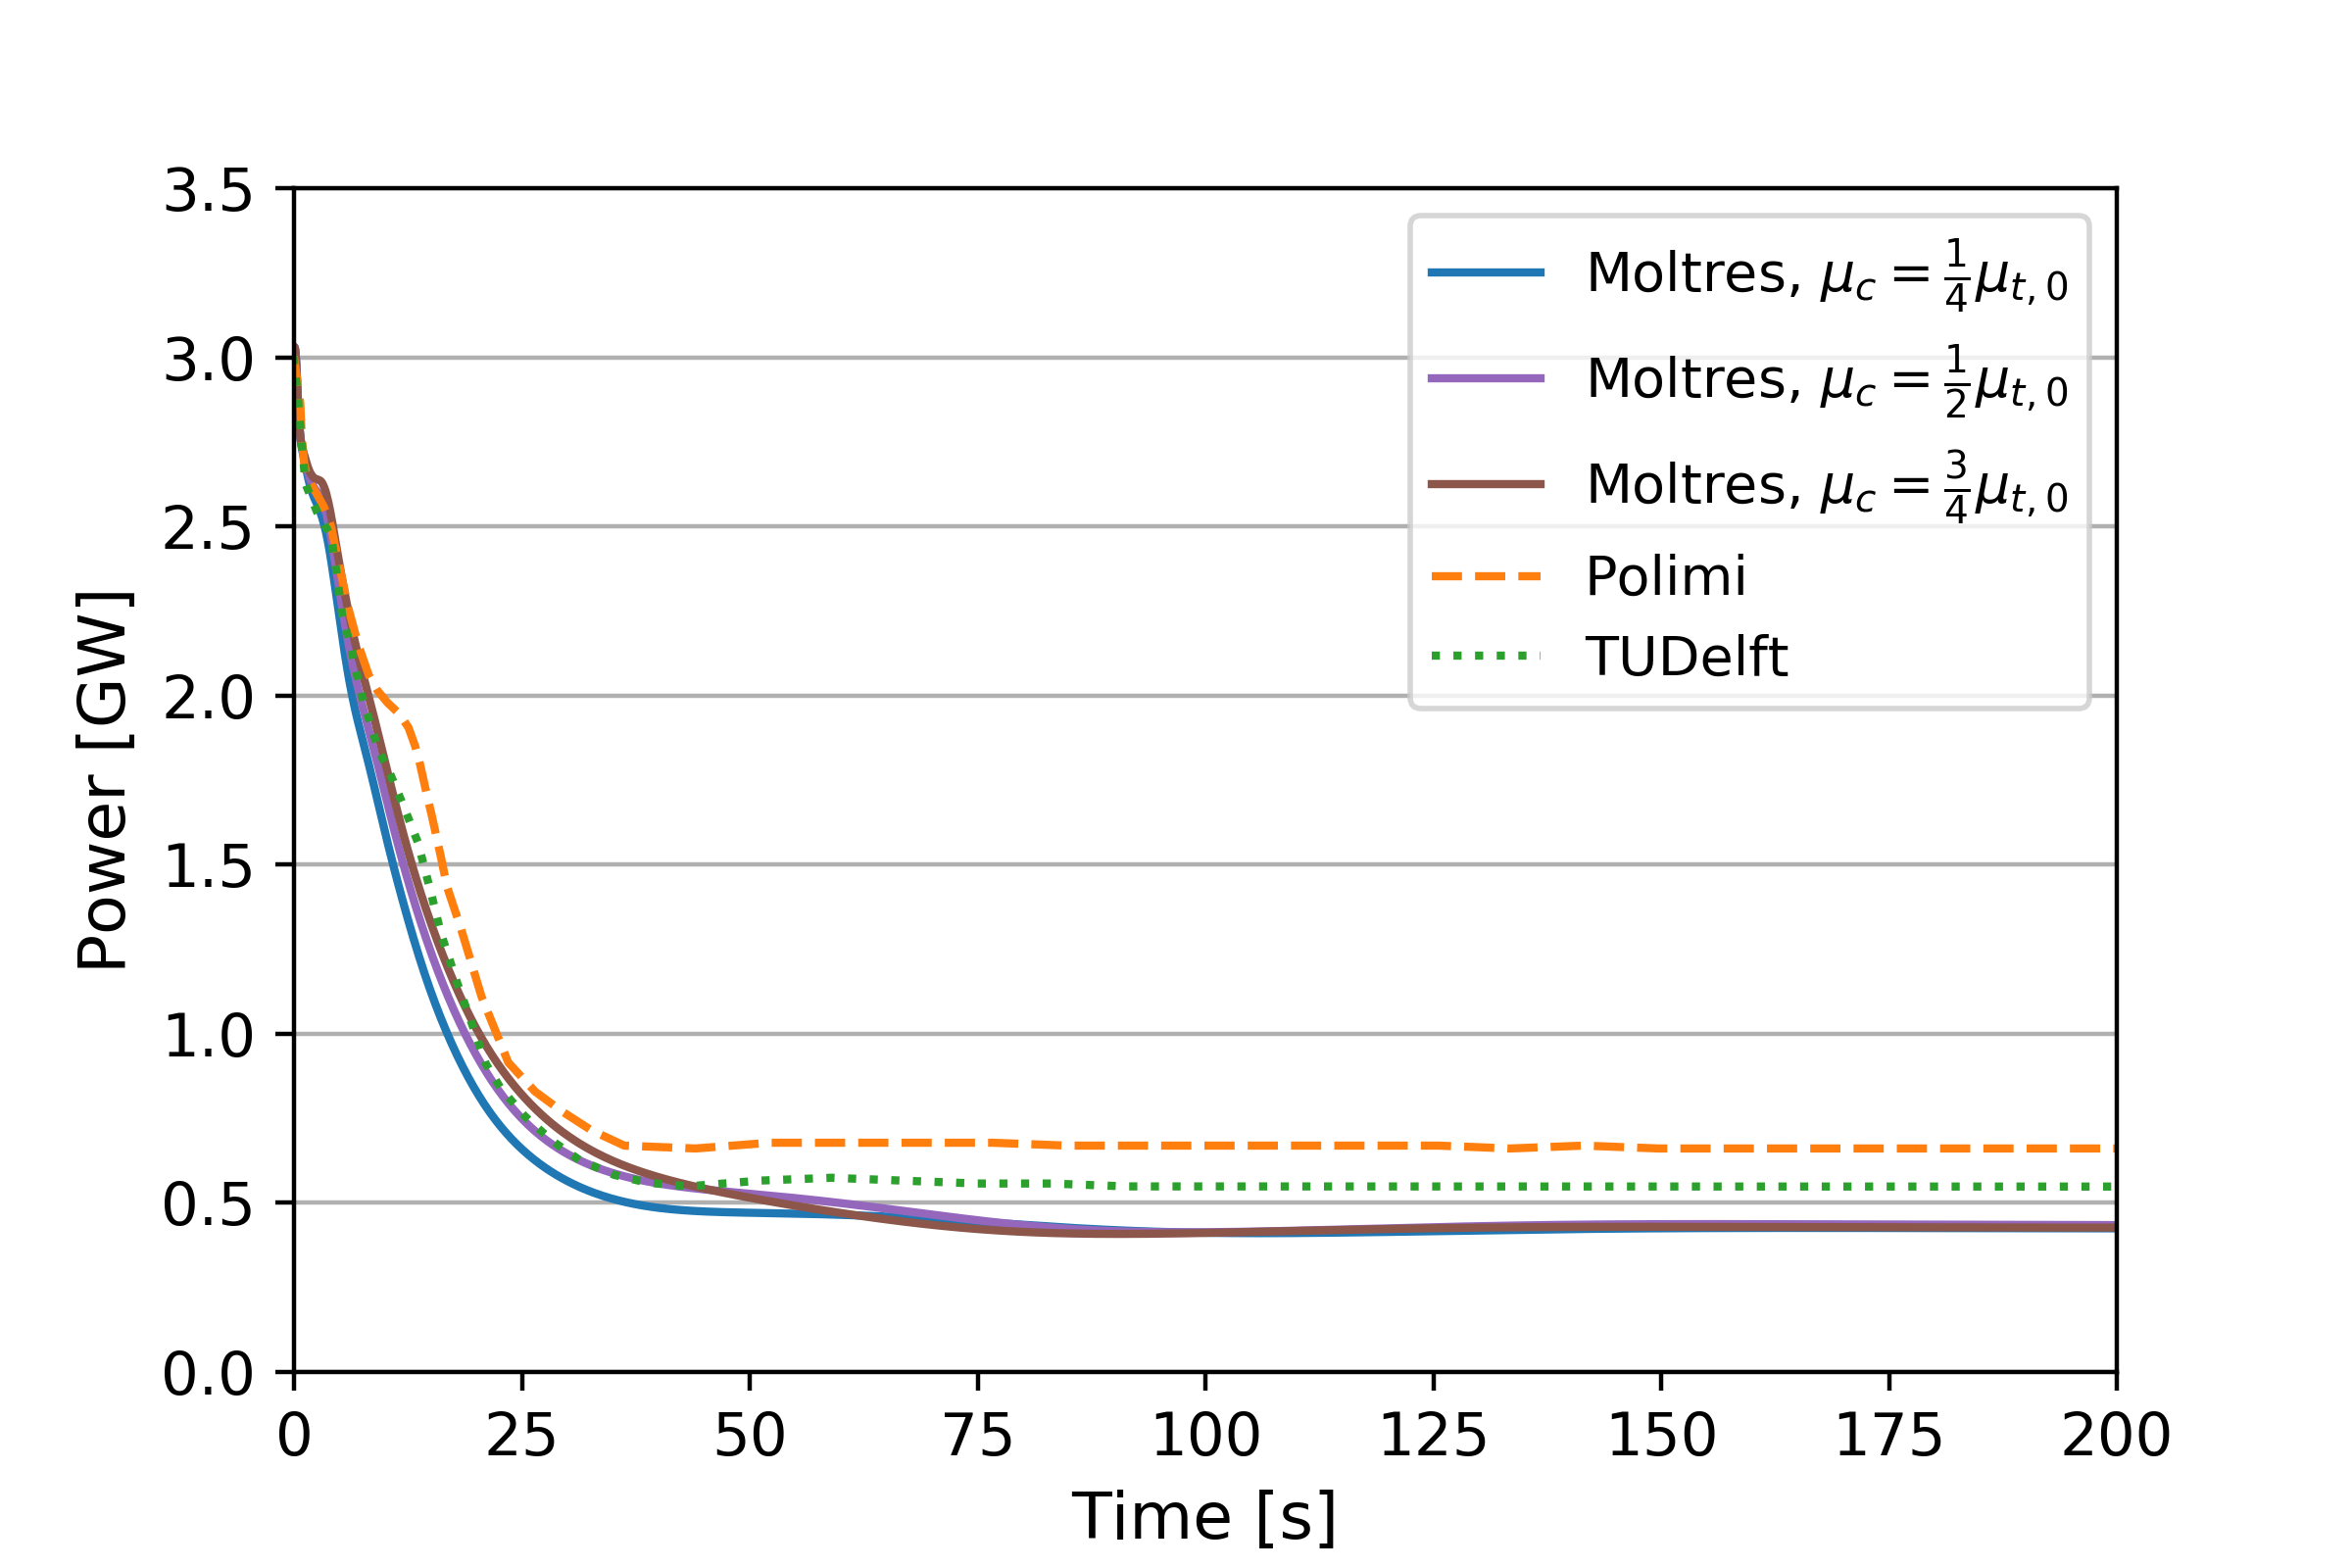
\includegraphics[width=\textwidth]{lof-heat}
    \end{subfigure}
    \hfill
    \begin{subfigure}[t]{.485\textwidth}
        \centering
        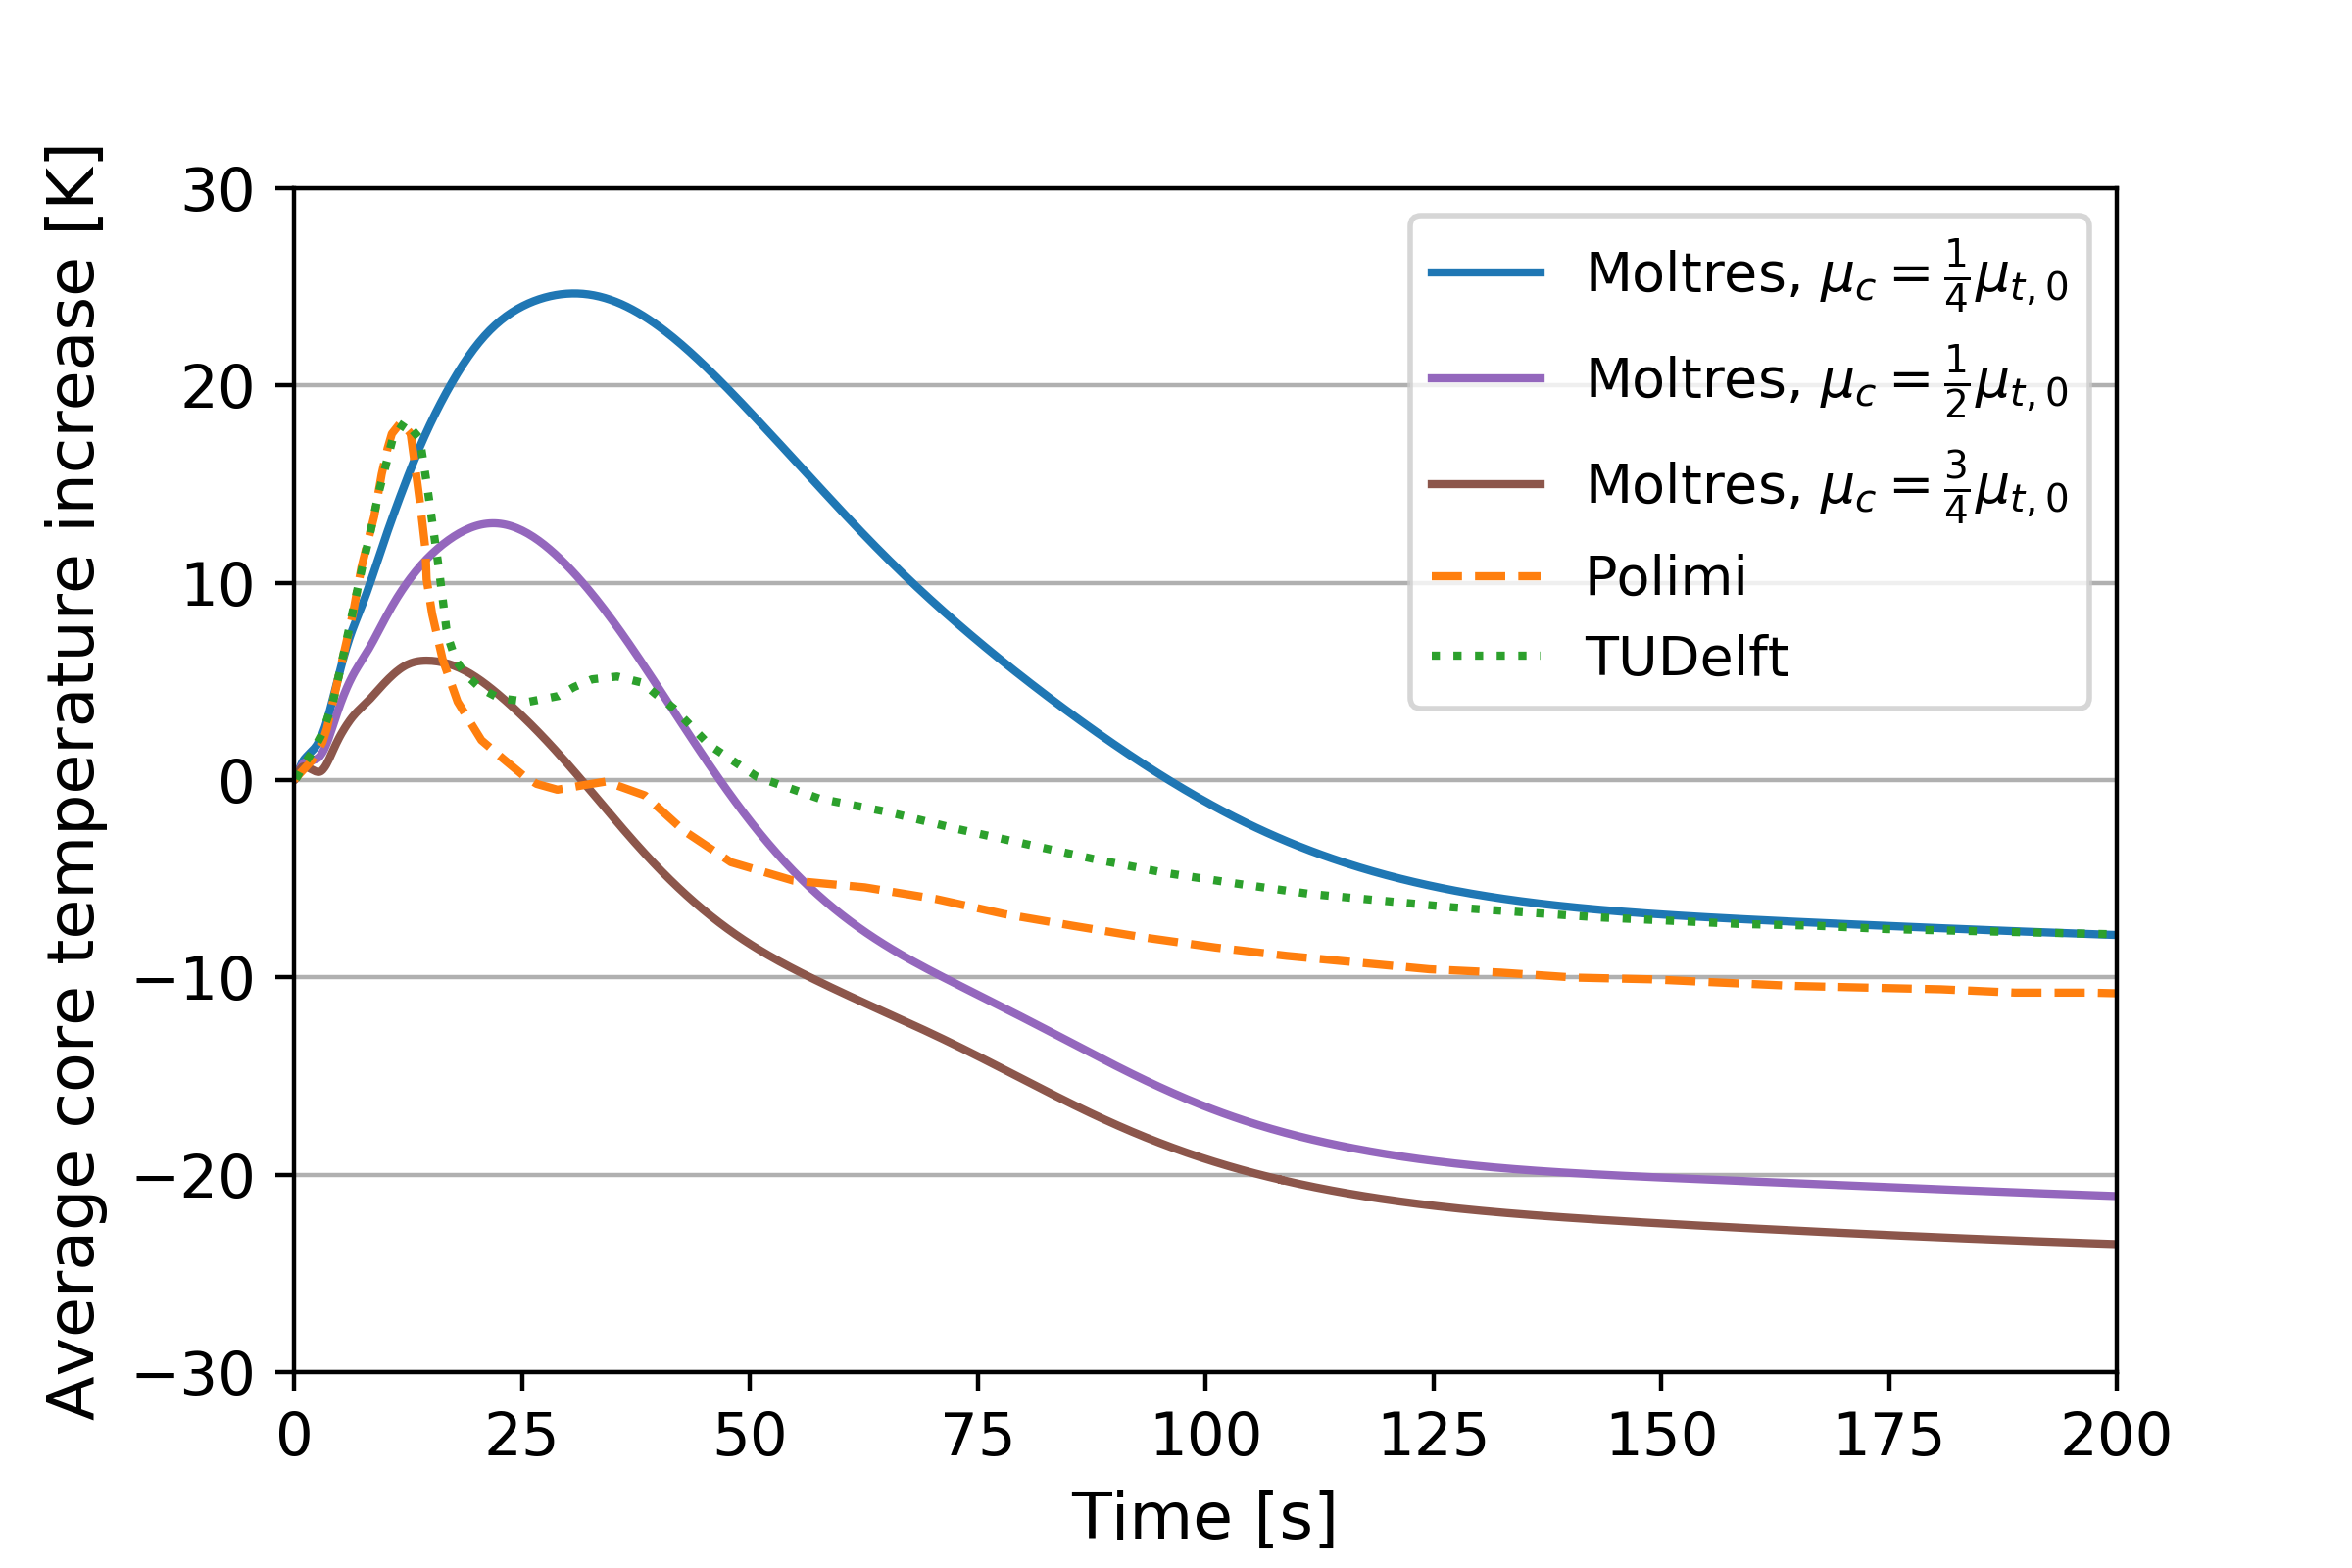
\includegraphics[width=\textwidth]{lof-temp}
    \end{subfigure}
    \caption{Power output and average core temperature increase during
    an unprotected loss of flow transient in the Moltres, PoliMi, and
    TU Delft models \cite{fiorina_modelling_2014}.}
    \label{fig:lof}
\end{figure}

\paragraph{Critical Assessment} \label{sec:msfr-critique}

Given the inherent and unique characteristics of \glspl{MSR}, the new
capabilities introduced in this work---coupling to incompressible Navier-Stokes
equations, precursor loop system, and decay heat model---are essential for
accurate \gls{MSR} modeling and simulation. This work demonstrated these
capabilities through steady-state and transient studies of a 2-D axisymmetric
\gls{MSFR} model similar to models by Fiorina et al.
\cite{fiorina_modelling_2014} and Aufiero et al.
\cite{aufiero_development_2014}. The Moltres model showed good agreement with
the other models in
most steady-state and transient cases with respect to the neutron flux, reactor
power, temperature, and velocity distributions. Most crucially, the
incompressible flow model reproduced characteristic regions of recirculating
flow and near-stagnant flow observed in the PoliMi and TU Delft \gls{MSFR}
models, which led to the formation of temperature hotspots and precursor
accumulation in the core.

However, significant discrepancies observed during pump-initiated transient
scenarios highlight the need for a proper turbulence model to capture
turbulent flow effects in some \gls{MSR} designs. Unlike the \gls{MSRE}, the
\gls{MSFR} experiences highly turbulent flow, whose Reynolds number is on the
order of $10^6$ under normal operating conditions. This level of turbulent flow
produces eddies of a wide range of length scales, and the computational demands
of the fine mesh and time resolution render it numerically unsolvable with
today's computational resources. Turbulence models allow for cheaper turbulence
simulations on coarser meshes by approximating the turbulent effects through
statistical analysis. Fiorina et al. \cite{fiorina_modelling_2014} employed the
$k$-$\epsilon$ turbulence model in their PoliMi and TU Delft models. Moltres
will benefit from coupling to similar intermediate-fidelity turbulence models
for turbulence simulations at reasonable computational costs.

While the Moltres model demonstrated good agreement with published data in the
steady-state, reactivity, and loss of heat sink scenarios, this work does not
thoroughly verify Moltres' capabilities for \gls{MSR} modeling.
The \gls{MSFR} simulations involve various physics models which combine to form
a complex multiphysics model. Therefore, it is difficult to pinpoint sources of
discrepancy with a high degree of certainty. Differences in the modeling
approaches also introduce discrepancies that cannot be reliably identified.
Moltres will benefit from code-to-code verification of
individual components responsible for modeling various physics present in
\glspl{MSR} and Moltres' multiphysics coupling approach.

\section{CNRS Benchmark}

As identified in Section \ref{sec:msfr-critique},
Moltres will benefit from further \gls{VV} of its
\gls{MSR} modeling capabilities. This chapter presents verification
results from Moltres for problems within the CNRS Benchmark
\cite{tiberga_results_2020}---a numerical benchmark specifically designed to
assess \gls{MSR} simulation tools on coupled multiphysics simulations of
fast-spectrum \glspl{MSR}. The benchmark consists of several steps in which
steady-state and transient simulations are prescribed. The benchmark starts with simple
single-physics cases and incrementally introduces various types of
multiphysics coupling until full coupling is simulated in the final steps. This
gradual approach helps participants identify sources of discrepancies
that can arise from differences in modeling assumptions or
cross-section libraries, or actual errors in the software. I adapted the
contents of this chapter from my journal article titled
``\textit{Verification of Moltres for Multiphysics Simulations of Fast-Spectrum
Molten Salt Reactors}'' and published in the Annals of Nuclear Energy journal
\cite{park_verification_2022}.

\subsection{Description of the CNRS Benchmark} \label{sec:benchmark}

The CNRS Benchmark \cite{tiberga_results_2020} is a numerical
benchmark for multiphysics software dedicated to modeling \glspl{MSR}. It
consists of three phases and eight steps in total. Each
step is a well-defined subproblem for systematically assessing the
capabilities of \gls{MSR} software and pinpointing sources of discrepancies
between software. Phase 0 consists of three single-physics problems in fluid
dynamics, neutronics, and temperature. Phase 1 consists
of four coupled steady-state problems. Lastly, Phase 2 consists of one
coupled, time-dependent problem.

\begin{figure}[htb!]
	\centering
	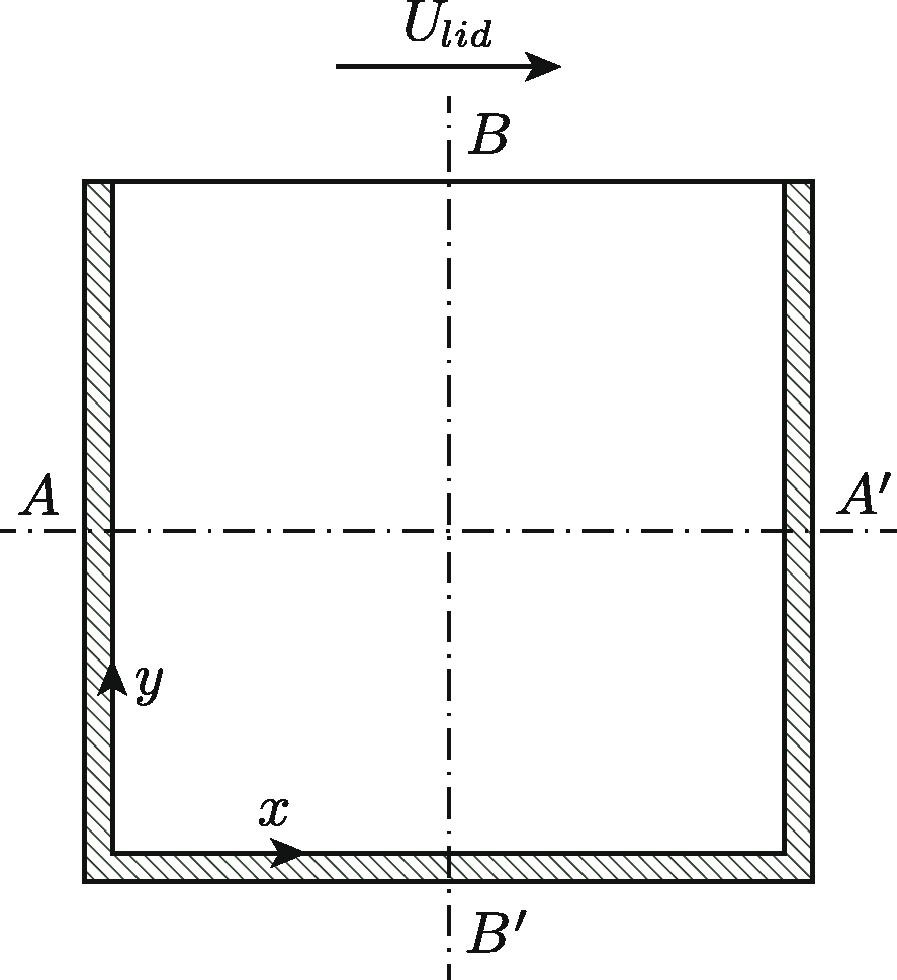
\includegraphics[width=.6\columnwidth]{cnrs-geometry}
	\caption{2m$\times$2m 2D domain of the CNRS Benchmark. $U_{lid}$
	represents the velocity along the top boundary. For comparison, various quantities are
	measured along the centerlines AA' and BB'. From Tiberga et
	al. \cite{tiberga_results_2020}.}
	\label{fig:cnrs-geometry}
\end{figure}

As shown in Figure \ref{fig:cnrs-geometry}, the domain geometry is a
2m$\times$2m square cavity filled with LiF-BeF$_2$-UF$_4$ molten salt at an
initial temperature of 900K \cite{tiberga_results_2020}.
Standard vacuum boundary conditions apply for neutron flux along all
boundaries whereby outgoing neutrons are considered lost, while homogeneous
boundary conditions apply for delayed neutron precursors. No-slip boundary
conditions apply for velocity variables in the cavity, except along the top
boundary for Steps 0.1, 0.3, 1.1, 1.2, and 1.4, which impose forced flow in the
form of lid-driven
cavity flow. For the temperature variable, all boundaries are insulated, and we
simulate salt cooling with the following volumetric heat sink equation:
%
\begin{align}
    q'''(\vec{r}) &= \gamma \left(900 - T(\vec{r})\right) \label{eq:cnrs-heat}
    \shortintertext{where}
    q''' &= \mbox{volumetric heat sink [W$\cdot$m$^{-3}$],}
    \nonumber \\
    \gamma &= \mbox{heat transfer coefficient [W$\cdot$m$^{-3}\cdot$K$^{-1}$],}
    \nonumber \\
    T(\vec{r}) &= \mbox{temperature at point $\vec{r}$ [K].} \nonumber
\end{align}

Tiberga et al. \cite{tiberga_results_2020} used Serpent 2
\cite{leppanen_serpent_2014} with the JEFF-3.1 library
\cite{koning_jeff-31_2006} to generate multigroup neutronics data for the
LiF-BeF$_2$-UF$_4$ salt in the domain at 900K, which they condensed into six
energy groups and eight precursor groups. We direct readers to their paper for
the group constant data \cite{tiberga_results_2020}. In addition, the
benchmark prescribes the following equations to govern the temperature
dependence in the cross sections and the neutron diffusion coefficients:
%
\begin{align}
    \Sigma_i (T) &= \Sigma_i(T_{ref})
    \frac{\rho_{fuel}(T)}{\rho_{fuel}(T_{ref})}
    \shortintertext{and}
    D (T) &= D(T_{ref})
    \frac{\rho_{fuel}(T_{ref})}{\rho_{fuel}(T)}
    \shortintertext{where}
    \Sigma_i &= \mbox{relevant macroscopic cross section [cm${-1}$],}
    \nonumber \\
    D &= \mbox{neutron diffusion coefficient [cm$^2\cdot$s$^{-1}$],}   
    \nonumber \\
    \rho_{fuel} &= \mbox{density of the fuel salt [kg$\cdot$m$^{-3}$],}
    \nonumber \\
    T_{ref} &= \mbox{reference temperature} = 900\mbox{ K}. \nonumber
\end{align}

The benchmark also prescribes incompressible Navier-Stokes flow with the
Boussinesq approximation for evaluating the salt flow in the
domain but does not restrict the type of neutronics model.
Table \ref{table:benchmark} lists the relevant input parameters and observables.

\begin{table*}[tp!]
	\caption{Input parameters and observables of each benchmark step.}
	\centering
	\footnotesize
    \begin{tabular}{p{.05\textwidth} p{.1\textwidth} p{.3\textwidth} p{.45\textwidth}}
		\toprule
        \textbf{Step} & \textbf{Name} & \textbf{Input parameters} & \textbf{Observables} \\
		\midrule
        0.1 & Velocity field &
		\begin{itemize}[nosep,noitemsep,left=0pt,
		                before={\begin{minipage}[t]{\hsize}},
                        after ={\end{minipage}}]
		    \item $U_{lid} = 0.5$ m$\cdot$s$^{-1}$
		\end{itemize}\vspace*{-\baselineskip}\mbox{} &
		\begin{itemize}[nosep,noitemsep,left=0pt,
		                before={\begin{minipage}[t]{\hsize}},
                        after ={\end{minipage}}]
		    \item Velocity components $(u_x,u_y)$ along AA' and BB'
		\end{itemize}\vspace*{-\baselineskip}\mbox{} \\
        \midrule
        0.2 & Neutronics &
        \begin{itemize}[nosep,noitemsep,left=0pt,
		                before={\begin{minipage}[t]{\hsize}},
                        after ={\end{minipage}}]
		    \item $U_{lid} = 0$ m$\cdot$s$^{-1}$
		    \item $T = 900$ K
		    \item $P = 1$ GW
		\end{itemize} &
		\begin{itemize}[nosep,noitemsep,left=0pt,
		                before={\begin{minipage}[t]{\hsize}},
                        after ={\end{minipage}}]
		    \item Fission rate density $\sum^6_g \Sigma_{f,g} \phi_g(\vec{r})$ along AA'
            \item Reactivity $\rho$
		\end{itemize}\vspace*{-\baselineskip}\mbox{} \\
        \midrule
        0.3 & Temperature &
        \begin{itemize}[nosep,noitemsep,left=0pt,
		                before={\begin{minipage}[t]{\hsize}},
                        after ={\end{minipage}}]
		    \item Fixed flow field from Step 0.1 for
		    $U_{lid} = 0.5$ m$\cdot$s$^{-1}$
		    \item Fixed heat source distribution
		    $\sum^6_{g} \epsilon_g \Sigma_{f,g} \phi_g(\vec{r})$ from Step 0.2
		    \item $\gamma = 10^6$ W$\cdot$m$^{-3}\cdot$K$^{-1}$
		\end{itemize} &
		\begin{itemize}[nosep,noitemsep,left=0pt,
		                before={\begin{minipage}[t]{\hsize}},
                        after ={\end{minipage}}]
		    \item Temperature $T$ along AA' and BB'
		\end{itemize}\vspace*{-\baselineskip}\mbox{} \\
        \midrule
        1.1 & Circulating fuel &
        \begin{itemize}[nosep,noitemsep,left=0pt,
		                before={\begin{minipage}[t]{\hsize}},
                        after ={\end{minipage}}]
		    \item Fixed flow field from Step 0.1 for
		    $U_{lid} = 0.5$ m$\cdot$s$^{-1}$
		    \item $T = 900$ K
		    \item $P = 1$ GW
		\end{itemize} &
		\begin{itemize}[nosep,noitemsep,left=0pt,
		                before={\begin{minipage}[t]{\hsize}},
                        after ={\end{minipage}}]
		    \item Delayed neutron source $\sum^8_i \lambda_i C_i$ along AA' and BB'
		    \item Reactivity change between Step 1.1 and Step 0.2,
		    $\Delta \rho = \rho - \rho_{s_{0.2}}$
		\end{itemize}\vspace*{-\baselineskip}\mbox{} \\
        \midrule
        1.2 & Power coupling &
        \begin{itemize}[nosep,noitemsep,left=0pt,
		                before={\begin{minipage}[t]{\hsize}},
                        after ={\end{minipage}}]
		    \item Fixed flow field from Step 0.1 for
		    $U_{lid} = 0.5$ m$\cdot$s$^{-1}$
		    \item $P = 1$ GW
		    \item $\gamma = 10^6$ W$\cdot$m$^{-3}\cdot$K$^{-1}$
		\end{itemize}\vspace*{-\baselineskip}\mbox{} &
		\begin{itemize}[nosep,noitemsep,left=0pt,
		                before={\begin{minipage}[t]{\hsize}},
                        after ={\end{minipage}}]
		    \item Temperature $T$ along AA' and BB'
            \item Reactivity change between Step 1.2 and Step 1.1,
            $\Delta\rho = \rho - \rho_{s_{1.1}}$
            \item Change in fission rate density
            $\sum^6_g \Sigma_{f,g} \phi_g(\vec{r}) -
            \left[\sum^6_g \Sigma_{f,g} \phi_g(\vec{r})\right]_{s_{0.2}}$
		\end{itemize} \\
        \midrule
        1.3 & Buoyancy &
        \begin{itemize}[nosep,noitemsep,left=0pt,
		                before={\begin{minipage}[t]{\hsize}},
                        after ={\end{minipage}}]
		    \item $P = 1$ GW
		    \item $U_{lid} = 0$ m$\cdot$s$^{-1}$
		    \item $\gamma = 10^6$ W$\cdot$m$^{-3}\cdot$K$^{-1}$
		\end{itemize}\vspace*{-\baselineskip}\mbox{} &
		\begin{itemize}[nosep,noitemsep,left=0pt,
		                before={\begin{minipage}[t]{\hsize}},
                        after ={\end{minipage}}]
		    \item Velocity components $(u_x, u_y)$ along AA' and BB'
            \item Temperature $T$ along AA' and BB'
            \item Delayed neutron source $\sum^8_i \lambda_i C_i$ along AA' and BB'
            \item Reactivity change from Step 0.2
        $\Delta\rho = \rho - \rho_{s_{0.2}}$
		\end{itemize} \\
        \midrule
        1.4 & Full coupling &
        \begin{itemize}[nosep,noitemsep,left=0pt,
		                before={\begin{minipage}[t]{\hsize}},
                        after ={\end{minipage}}]
		    \item $\gamma = 10^6$ W$\cdot$m$^{-3}\cdot$K$^{-1}$
		    \item $P$ variable in the range $[0,1]$ GW with a step of 0.2 GW
		    \item $U_{lid}$ variable in the range $[0,0.5]$ m$\cdot$s$^{-1}$
		    with a step of 0.1 m$\cdot$s$^{-1}$
		\end{itemize} &
		\begin{itemize}[nosep,noitemsep,left=0pt,
		                before={\begin{minipage}[t]{\hsize}},
                        after ={\end{minipage}}]
		    \item Reactivity change between Step 1.4 and Step 0.2,
		    $\Delta\rho = \rho - \rho_{s_{0.2}}$, for all permutations of $P$
		    and $U_{lid}$ values
		\end{itemize}\vspace*{-\baselineskip}\mbox{} \\
        \midrule
        2.1 & Forced convection transient &
        \begin{itemize}[nosep,noitemsep,left=0pt,
		                before={\begin{minipage}[t]{\hsize}},
                        after ={\end{minipage}}]
		    \item $\gamma = 10^6$ W$\cdot$m$^{-3}\cdot$K$^{-1}$
            \item Steady-state solution from Step 1.4 for $U_{lid} = 0.5$
        m$\cdot$s$^{-1}$ and $P = 1.0$ GW
		\end{itemize} &
		\begin{itemize}[nosep,noitemsep,left=0pt,
		                before={\begin{minipage}[t]{\hsize}},
                        after ={\end{minipage}}]
		    \item Power gain and shift as a function of the perturbation frequency
		\end{itemize}\vspace*{-\baselineskip}\mbox{} \\
		\bottomrule
	\end{tabular}
	\label{table:benchmark}
\end{table*}

Step 2.1 studies the transient response of the fully coupled nonlinear system.
Linear perturbation analyses are performed by introducing periodic
perturbations to the heat transfer coefficient $\gamma$ and studying the gain
and phase shift of the response in the total power $P$. For the initial
conditions, the steady-state solution from Step 1.4 with
$U_{lid} = 0.5$ m$\cdot$s$^{-1}$ and $P = 1$ GW is used. This initial
configuration is made exactly critical by scaling the neutron source terms,
from fission and \gls{DNP} decay, by the inverse of the criticality eigenvalue
solution from Step 1.4.

$\gamma$ is uniformly perturbed according to small-amplitude sine waves given
as:
%
\begin{align}
    \gamma =& \gamma_0 \left[ 1 + 0.1\sin\left(2 \pi f \right) \right]
    \shortintertext{where}
    \gamma_0 =& 10^6 \mbox{ W$\cdot$m$^{-3}\cdot$K$^{-1}$}, \nonumber \\
    f \in& \left\lbrace 0.0125, 0.025, 0.05, 0.1, 0.2, 0.4, 0.8 \right\rbrace 
    \mbox{ Hz.} \nonumber
\end{align}

The benchmark defines power gain as:
%
\begin{align}
    \mbox{Power gain} =& \frac{\left(P_{max} - P_{avg}\right)/P_{avg}}{
    \left(\gamma_{max} - \gamma_{avg}\right)/\gamma_{avg}}
\end{align}
%
The subscripts denote the maximum and time-averaged values of $P$ and $\gamma$.

\FloatBarrier

\subsection{Modeling Approach with Moltres} \label{sec:model}

This section describes the specific modeling approach for
simulating the CNRS Benchmark cases in Moltres.

For this work\footnote{The input files for
all benchmark
cases are available on the Moltres GitHub repository at 
\url{https://github.com/arfc/moltres/tree/devel/problems/2021-cnrs-benchmark}.
}, I ran the benchmark cases on a uniformly-spaced mesh
of 200$\times$200 elements. Thus, the dimensions of each mesh element are
0.01m$\times$0.01m. I adopted the group constant data
provided by Tiberga et al. \cite{tiberga_results_2020}. Next, I
discretized most variables, i.e., neutron fluxes, velocity
components, pressure, and temperature, using continuous, first-order, Lagrange
shape functions. The only exception is the precursor concentration variables,
which I discretized using zeroth-order monomial shape functions and solved
using a \gls{DFEM}. I interpolated the resulting discontinuous,
cell-centered precursor values to obtain the nodal values for results
analysis.

The
\texttt{Navier-Stokes} and \texttt{Heat} \texttt{Conduction} modules from
\gls{MOOSE} provide some of the capabilities for
modeling incompressible flow and heat transfer. In particular, I stabilized
the incompressible flow and temperature governing equations using the
\gls{SUPG} stabilization method implemented in \gls{MOOSE}
\cite{peterson_overview_2018}. Without \gls{SUPG} stabilization, I
observed spurious numerical oscillations in the velocity and temperature near
the top boundary due to the singularity on the top left corner where different
velocity boundary conditions meet. I also applied the \gls{PSPG} stabilization
scheme \cite{hughes_new_1986} from the Navier-Stokes module
\cite{peterson_overview_2018},
which enables equal-order discretizations in the velocity and pressure
variables. Equal-order discretizations with \gls{PSPG} are computationally
cheaper and more convenient than implementing higher-order
velocity discretizations for stability without \gls{PSPG}
\cite{chapelle_inf-sup_1993}.

Using the inverse power method solver in \gls{MOOSE}, I ran all eigenvalue calculations in
Steps 0.2, 1.1, 1.2, 1.3, and 1.4. I ran all other steps
using the Preconditioned Newton-Krylov solver
\cite{gaston_physics-based_2015}. The coupled steady-state problems in
Steps 1.2, 1.3, and 1.4 required segregated solvers for the neutronics
and the thermal-hydraulics due to the unique problem setups involving a
criticality search problem for the neutron multiplication factor
and a steady-state problem in thermal-hydraulics simultaneously.

\begin{table}[tb]
    \caption{Timestep sizes used for the time-dependent cases in
    Step 2.1, corresponding to 1/200th of the perturbation period.}
	\centering
	\setlength\tabcolsep{2.5pt}
	\begin{tabular}{l l l l l l l l}
	    \toprule
	    Frequency [Hz] & 0.0125 & 0.025 & 0.05 & 0.1 & 0.2 & 0.4 & 0.8 \\
	    \midrule
	    Timestep size [s] & 0.2 & 0.2 & 0.1 & 0.05 & 0.025 & 0.0125 & 0.00625
	    \\
	    \bottomrule
	\end{tabular}
	\label{table:timestep}
\end{table}

For the time-dependent cases in Step 2.1, I employed full coupling with
a second-order implicit Backward Differential Formula (BDF2) time-stepping
scheme. I set the timestep sizes for each driving frequency in the heat transfer
coefficient to 1/200th of the perturbation period. Table
\ref{table:timestep} shows the timestep sizes. I assumed the
systems reached asymptotic behavior when the magnitudes of neighboring power
peaks differed by less than 0.001\% for at least ten wavelengths. Under this
assumption, the phase shift measurements between adjacent waves always
converged before the magnitude measurements of the power peaks.

Table \ref{table:software} compares the numerical methods, meshing schemes, and
neutronics models of Moltres and the four participating software packages in
the CNRS benchmark paper \cite{tiberga_results_2020}. The $SP_N$ and
$S_N$ neutronics models refer to the simplified $P_N$ spherical harmonics and
$S_N$ discrete ordinates neutron transport models, respectively. Based on the
solvers and methods of solution, Moltres is most similar to the
PHANTOM-$S_N$ + DGFlows \cite{tiberga_discontinuous_2019} multiphysics package
from \gls{TUD} with the $S_2$ neutron transport model. Participants from
\gls{CNRS} and \gls{PSI}
employed non-uniform meshes which were refined near the boundaries. In contrast,
we and the \gls{PoliMi} and \gls{TUD} participants employed uniform meshes.

\FloatBarrier

\begin{landscape}
\begin{table*}[p]
    \caption{List of software packages and their corresponding model
    specifications for the CNRS Benchmark simulations
    \cite{tiberga_results_2020}.}
    \centering
    \begin{tabular}{p{4.2cm} p{7cm} p{3.3cm} p{2cm} p{2.7cm}}
        \toprule
        Software & Institute & Numerical method & Mesh & Neutronics model \\
        \midrule
        OpenFOAM & Centre national de la recherche scientifique (CNRS) & Finite volume & 200$\times$200 \newline Non-uniform & $SP_1$ \& $SP_3$ \\
        OpenFOAM & Politecnico di Milano (PoliMi) & Finite volume & 400$\times$400 \newline Uniform & Neutron diffusion \\
        GeN-Foam & Paul Scherrer Institute (PSI) & Finite volume & 200$\times$200 \newline Non-uniform & Neutron diffusion \\
        PHANTOM-$S_N$+DGFlows & Delft University of Technology (TUD) & Discontinuous finite \newline element & 50$\times$50 \newline Uniform & $S_2$ \& $S_6$ \\
        Moltres (This work) & University of Illinois at Urbana-Champaign (UIUC) & Continuous \& discontinuous finite element & 200$\times$200 \newline Uniform & Neutron diffusion \\
        \bottomrule
    \end{tabular}
    \label{table:software}
\end{table*}
\end{landscape}

\FloatBarrier

\subsection{Results \& Discussion}

In this section, we compare the results from Moltres for each CNRS Benchmark
step to the results in the benchmark paper \cite{tiberga_results_2020}.
The software packages from \gls{CNRS} and \gls{TUD}
each report two sets of results from different angular discretizations
in their neutronics models for Steps 0.2, 1.1, 1.2, 1.3, 1.4, and 2.1. These
sets of results are labeled as CNRS-$SP_1$ and
CNRS-$SP_3$; and TUD-$S_2$ and TUD-$S_6$, respectively. The
authors performed code-to-code verification by sampling observable values at
201 equidistant points along the centerlines AA' and BB' and reporting the
discrepancy $\epsilon_c$ of each observable from each software
(indexed by $c$) for each measured observable $Q_c$ (not to be confused with
fission heat source $Q_f$), relative to the average of
that same observable $Q_{avg}$ from all participating software. Variables
$\epsilon_c$ and $Q_{avg}$ are calculated as:
%
\begin{align}
    \epsilon_c =& \sqrt{\frac{\sum^{N_p}_{i=1}\left[Q_c(\vec{r_i}) - Q_{avg}
    (\vec{r_i})\right]^2}{\sum^{N_p}_{i=1} Q^2_{avg}(\vec{r_i})}}
    \shortintertext{and}
    Q_{avg}(\vec{r_i}) =& \frac{1}{N_c} \sum^{N_c}_{c=1} Q_c(\vec{r_i})
    \shortintertext{where}
    Q_c(\vec{r_i}) =&
    \mbox{ value of observable $Q$ at location $\vec{r_i}$ from software $c$,}
    \nonumber \\
    N_p =& \mbox{ number of sampling points of quantity $Q$} = 201,
    \nonumber \\
    N_c =& \mbox{ number of participating software packages.} \nonumber
\end{align}

The average discrepancy $\epsilon$ across all software is calculated as:
%
\begin{align}
    \epsilon =& \frac{1}{N_c}\sum^{N_c}_{c=1} \epsilon_c
\end{align}

We adopted the averaged values $\epsilon$ and $Q_{avg}$ directly from the
reference work \cite{tiberga_results_2020} without including our results
in the calculations. We note that the benchmark does not provide a reference
solution, and a significantly erroneous value from one of the software packages
could heavily skew the discrepancy values. Nevertheless, the benchmark paper
reports good agreement among their software packages.

For observables measured along the centerlines AA' and BB', Tables
\ref{table:disc0} and \ref{table:disc1} report the discrepancy $\epsilon_c$ of
each observable from Moltres relative to the average of the benchmark
participants $Q_{avg}$ alongside the average discrepancy $\epsilon$ of
the benchmark participants. We also reproduce corresponding plots
in the benchmark paper for every observable along AA' or BB' in Figures
\ref{fig:0.1}, \ref{fig:0.2}, \ref{fig:0.3}, \ref{fig:1.1}, \ref{fig:1.2},
\ref{fig:1.3}, and \ref{fig:2.1} for a qualitative comparison of the results
from Moltres and the benchmark participants. Given the significant overlap in
the plot curves, these figures omit results from CNRS-$SP_1$ and TUD-$S_2$ to
reduce cluttering. The full dataset
of all observable results used in this results analysis is
available at \cite{park_results_2021}. Lastly, Table
\ref{table:rho} reports all reactivity and reactivity changes from
Steps 0.2, 1.1, 1.2, and 1.3.

\begin{figure}[h]
	\centering
    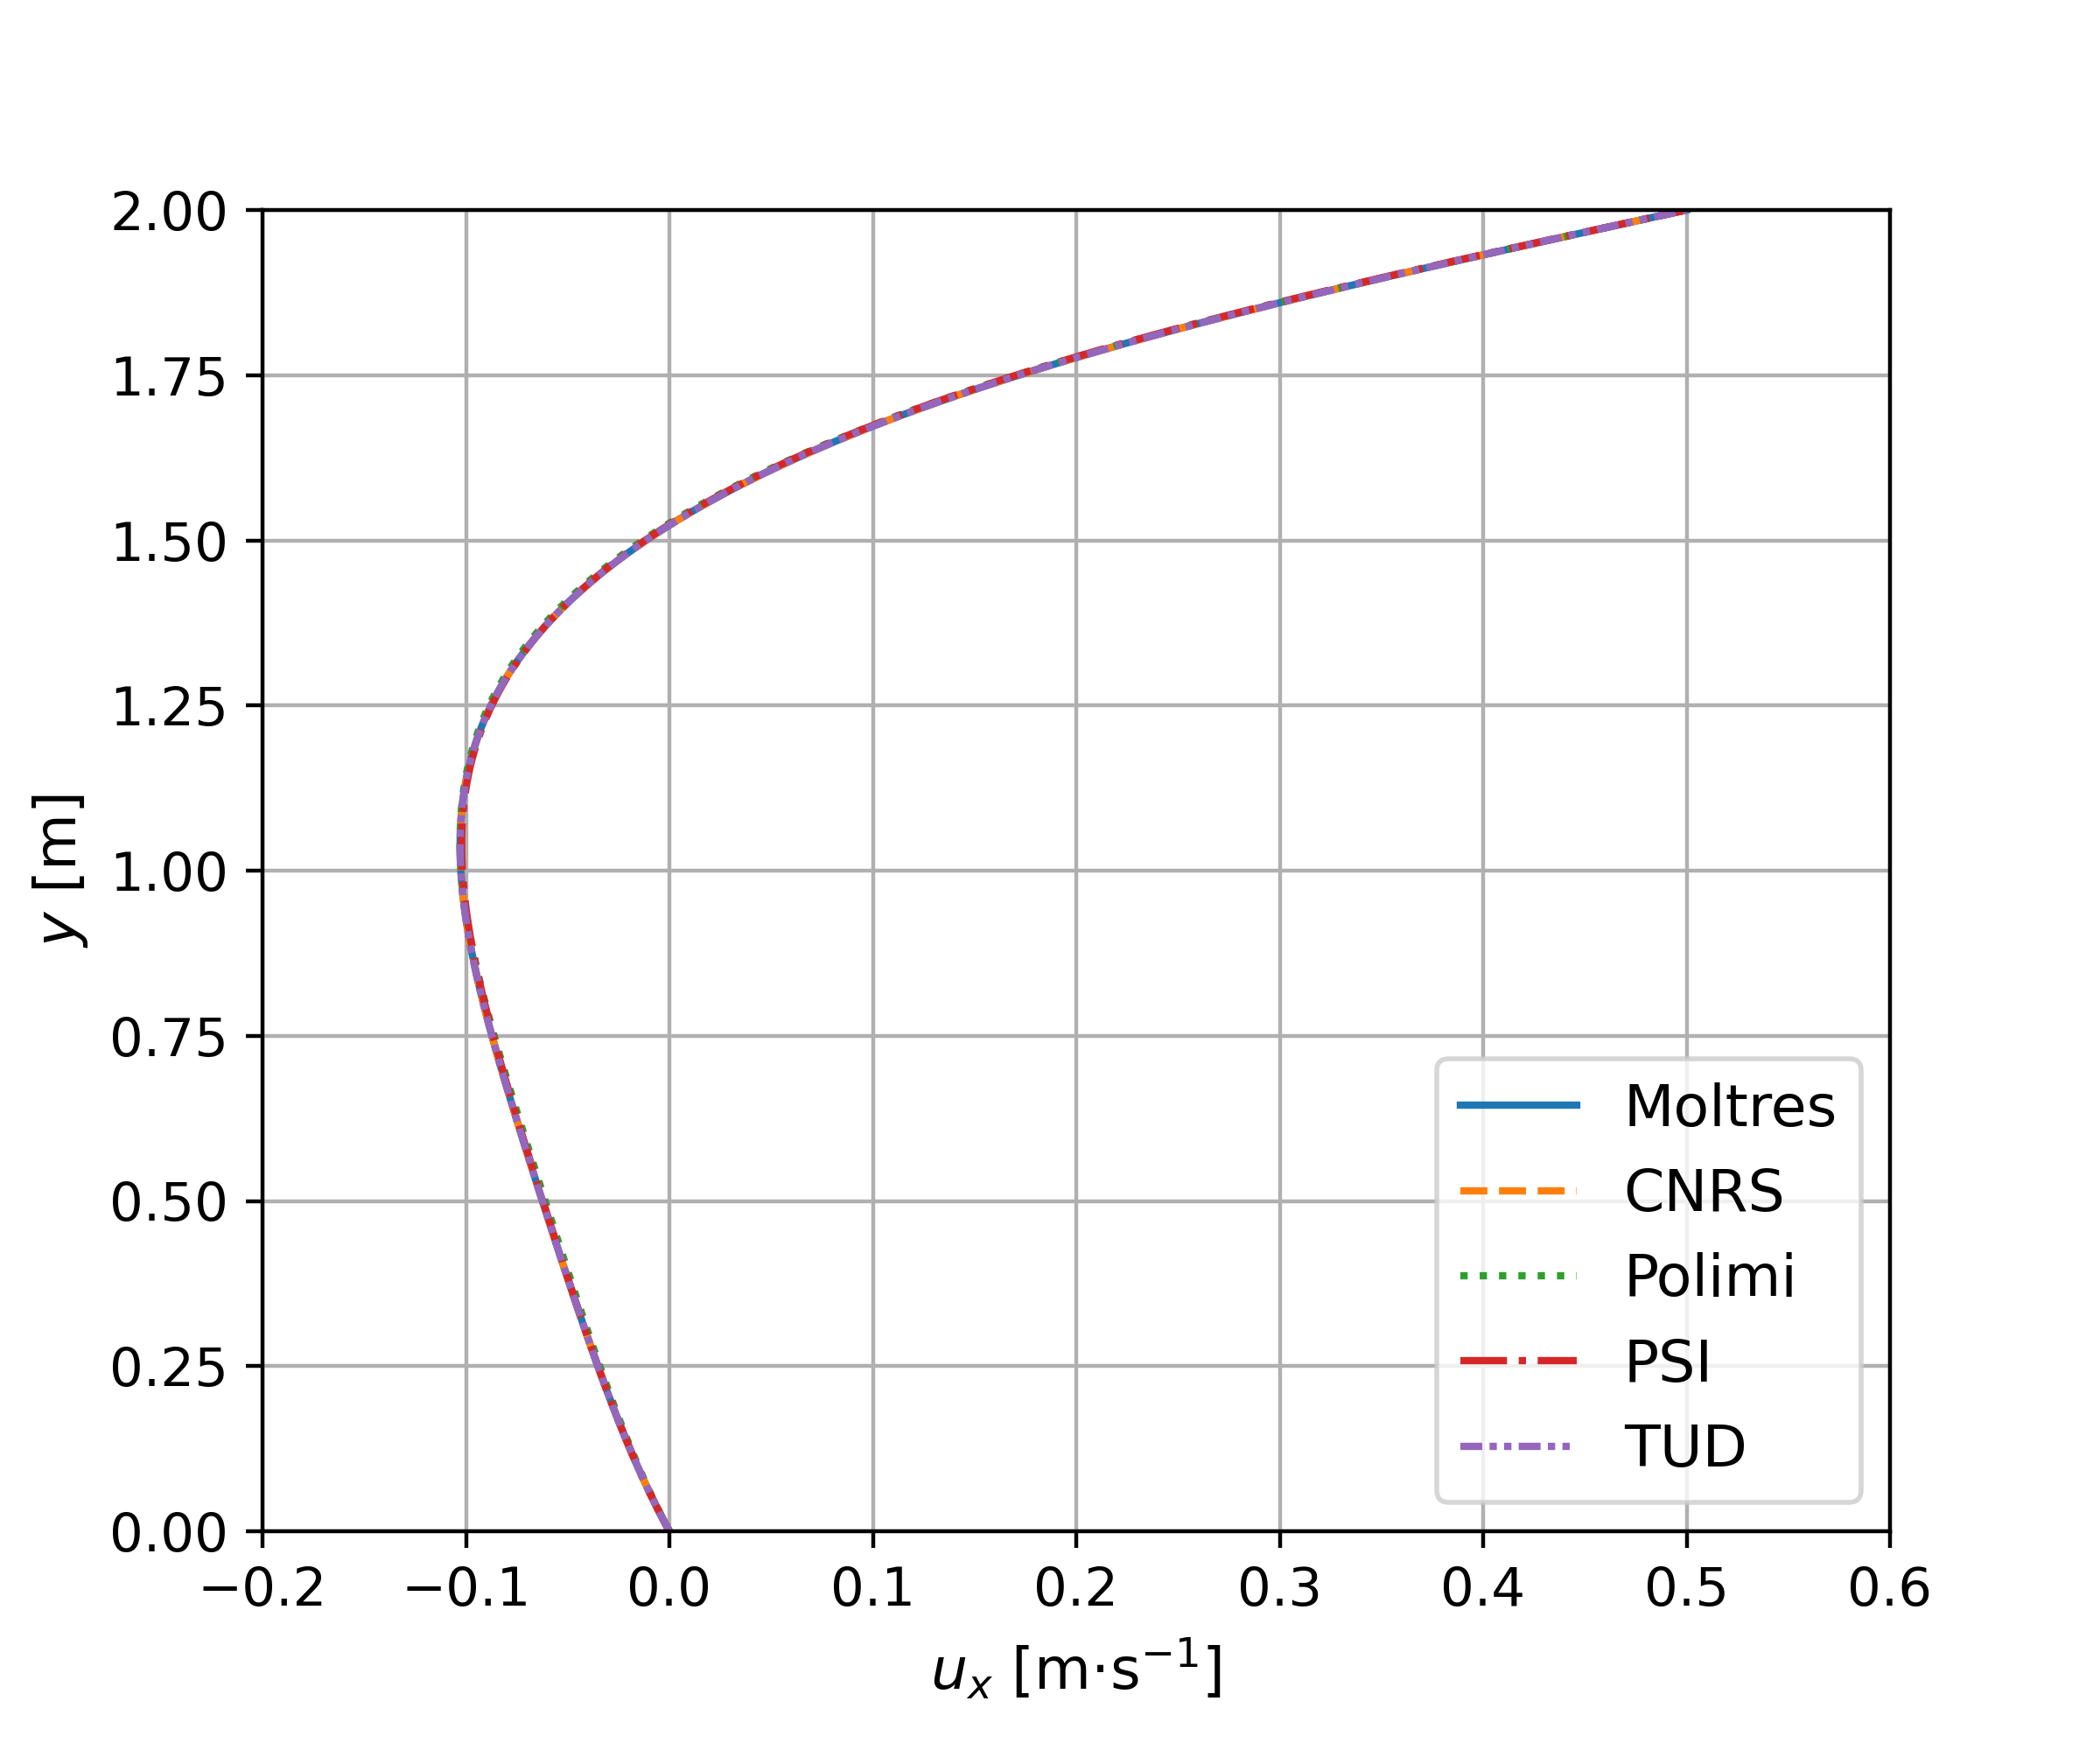
\includegraphics[width=.49\columnwidth]{0-1-vel-plot}
	\caption{Step 0.1 \textemdash\ Horizontal velocity component along BB'.}
	\label{fig:0.1}
\end{figure}
%
\begin{figure}[h]
	\centering
    \begin{subfigure}[b]{.49\textwidth}
      \centering
	  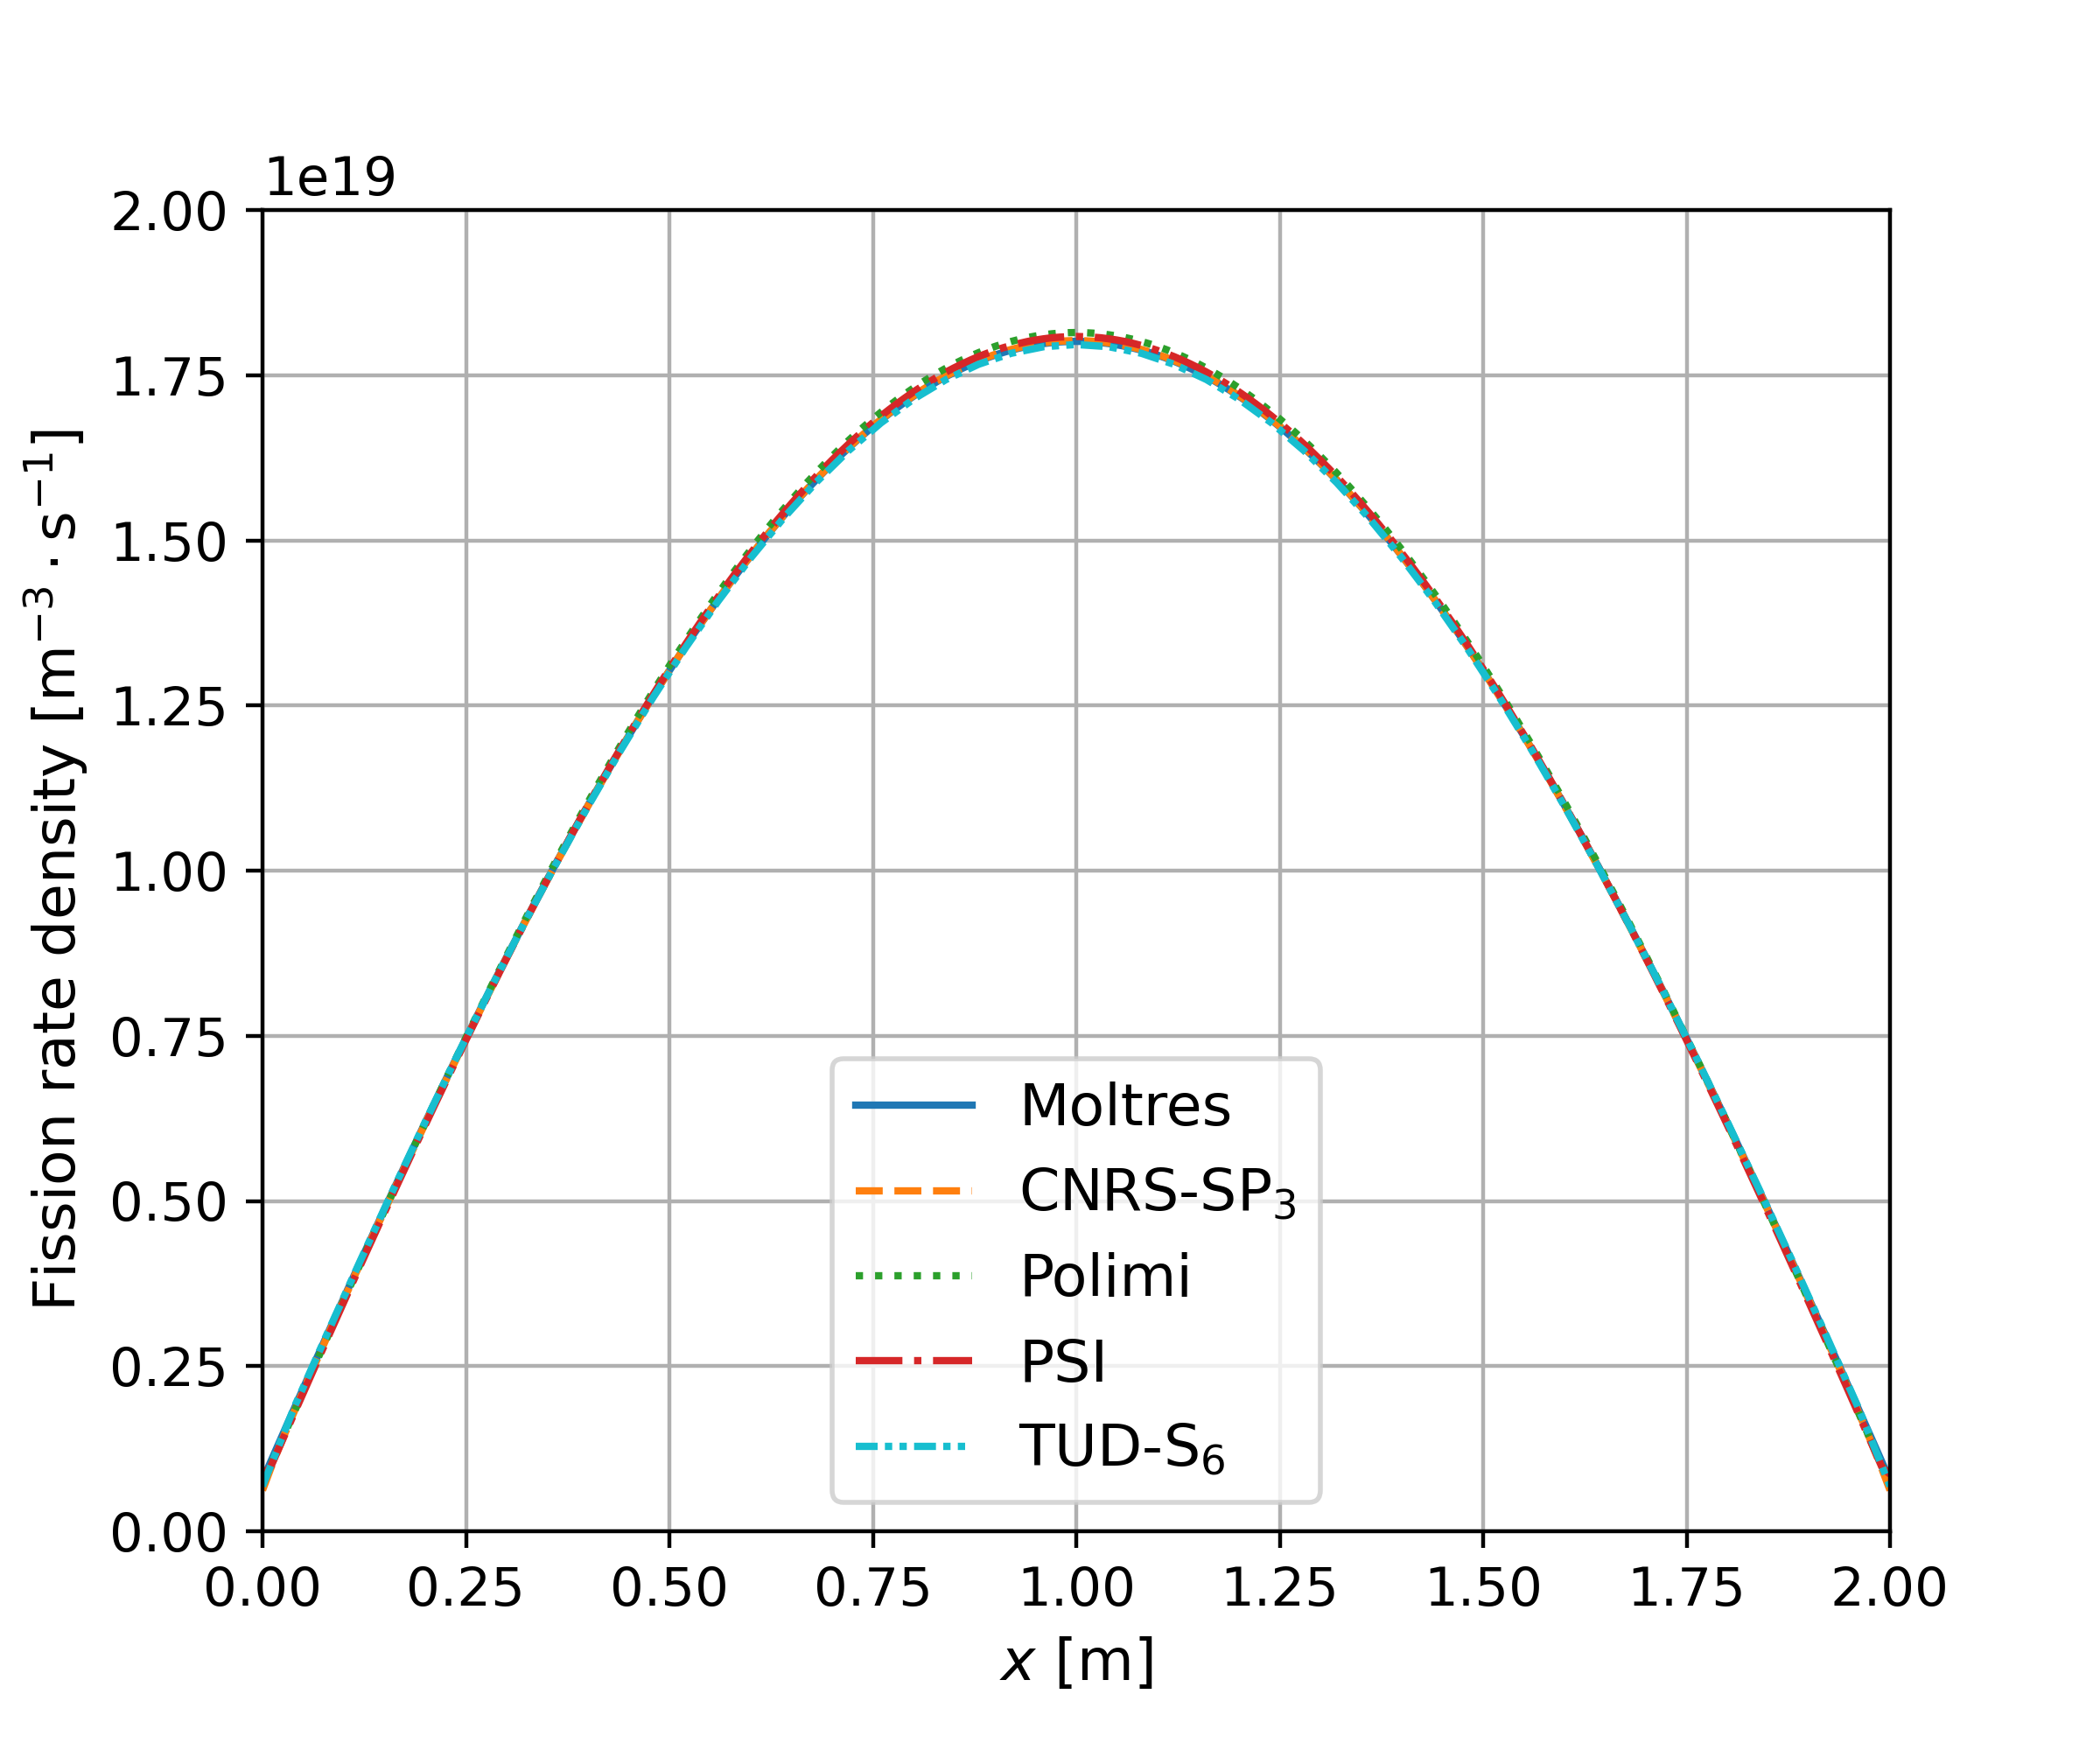
\includegraphics[width=\columnwidth]{0-2-fiss-plot}
	  \caption{Step 0.2 \textemdash\ Fission rate density along AA'.}
	  \label{fig:0.2}
    \end{subfigure}
    \hfill
    \begin{subfigure}[b]{.49\textwidth}
      \centering
	  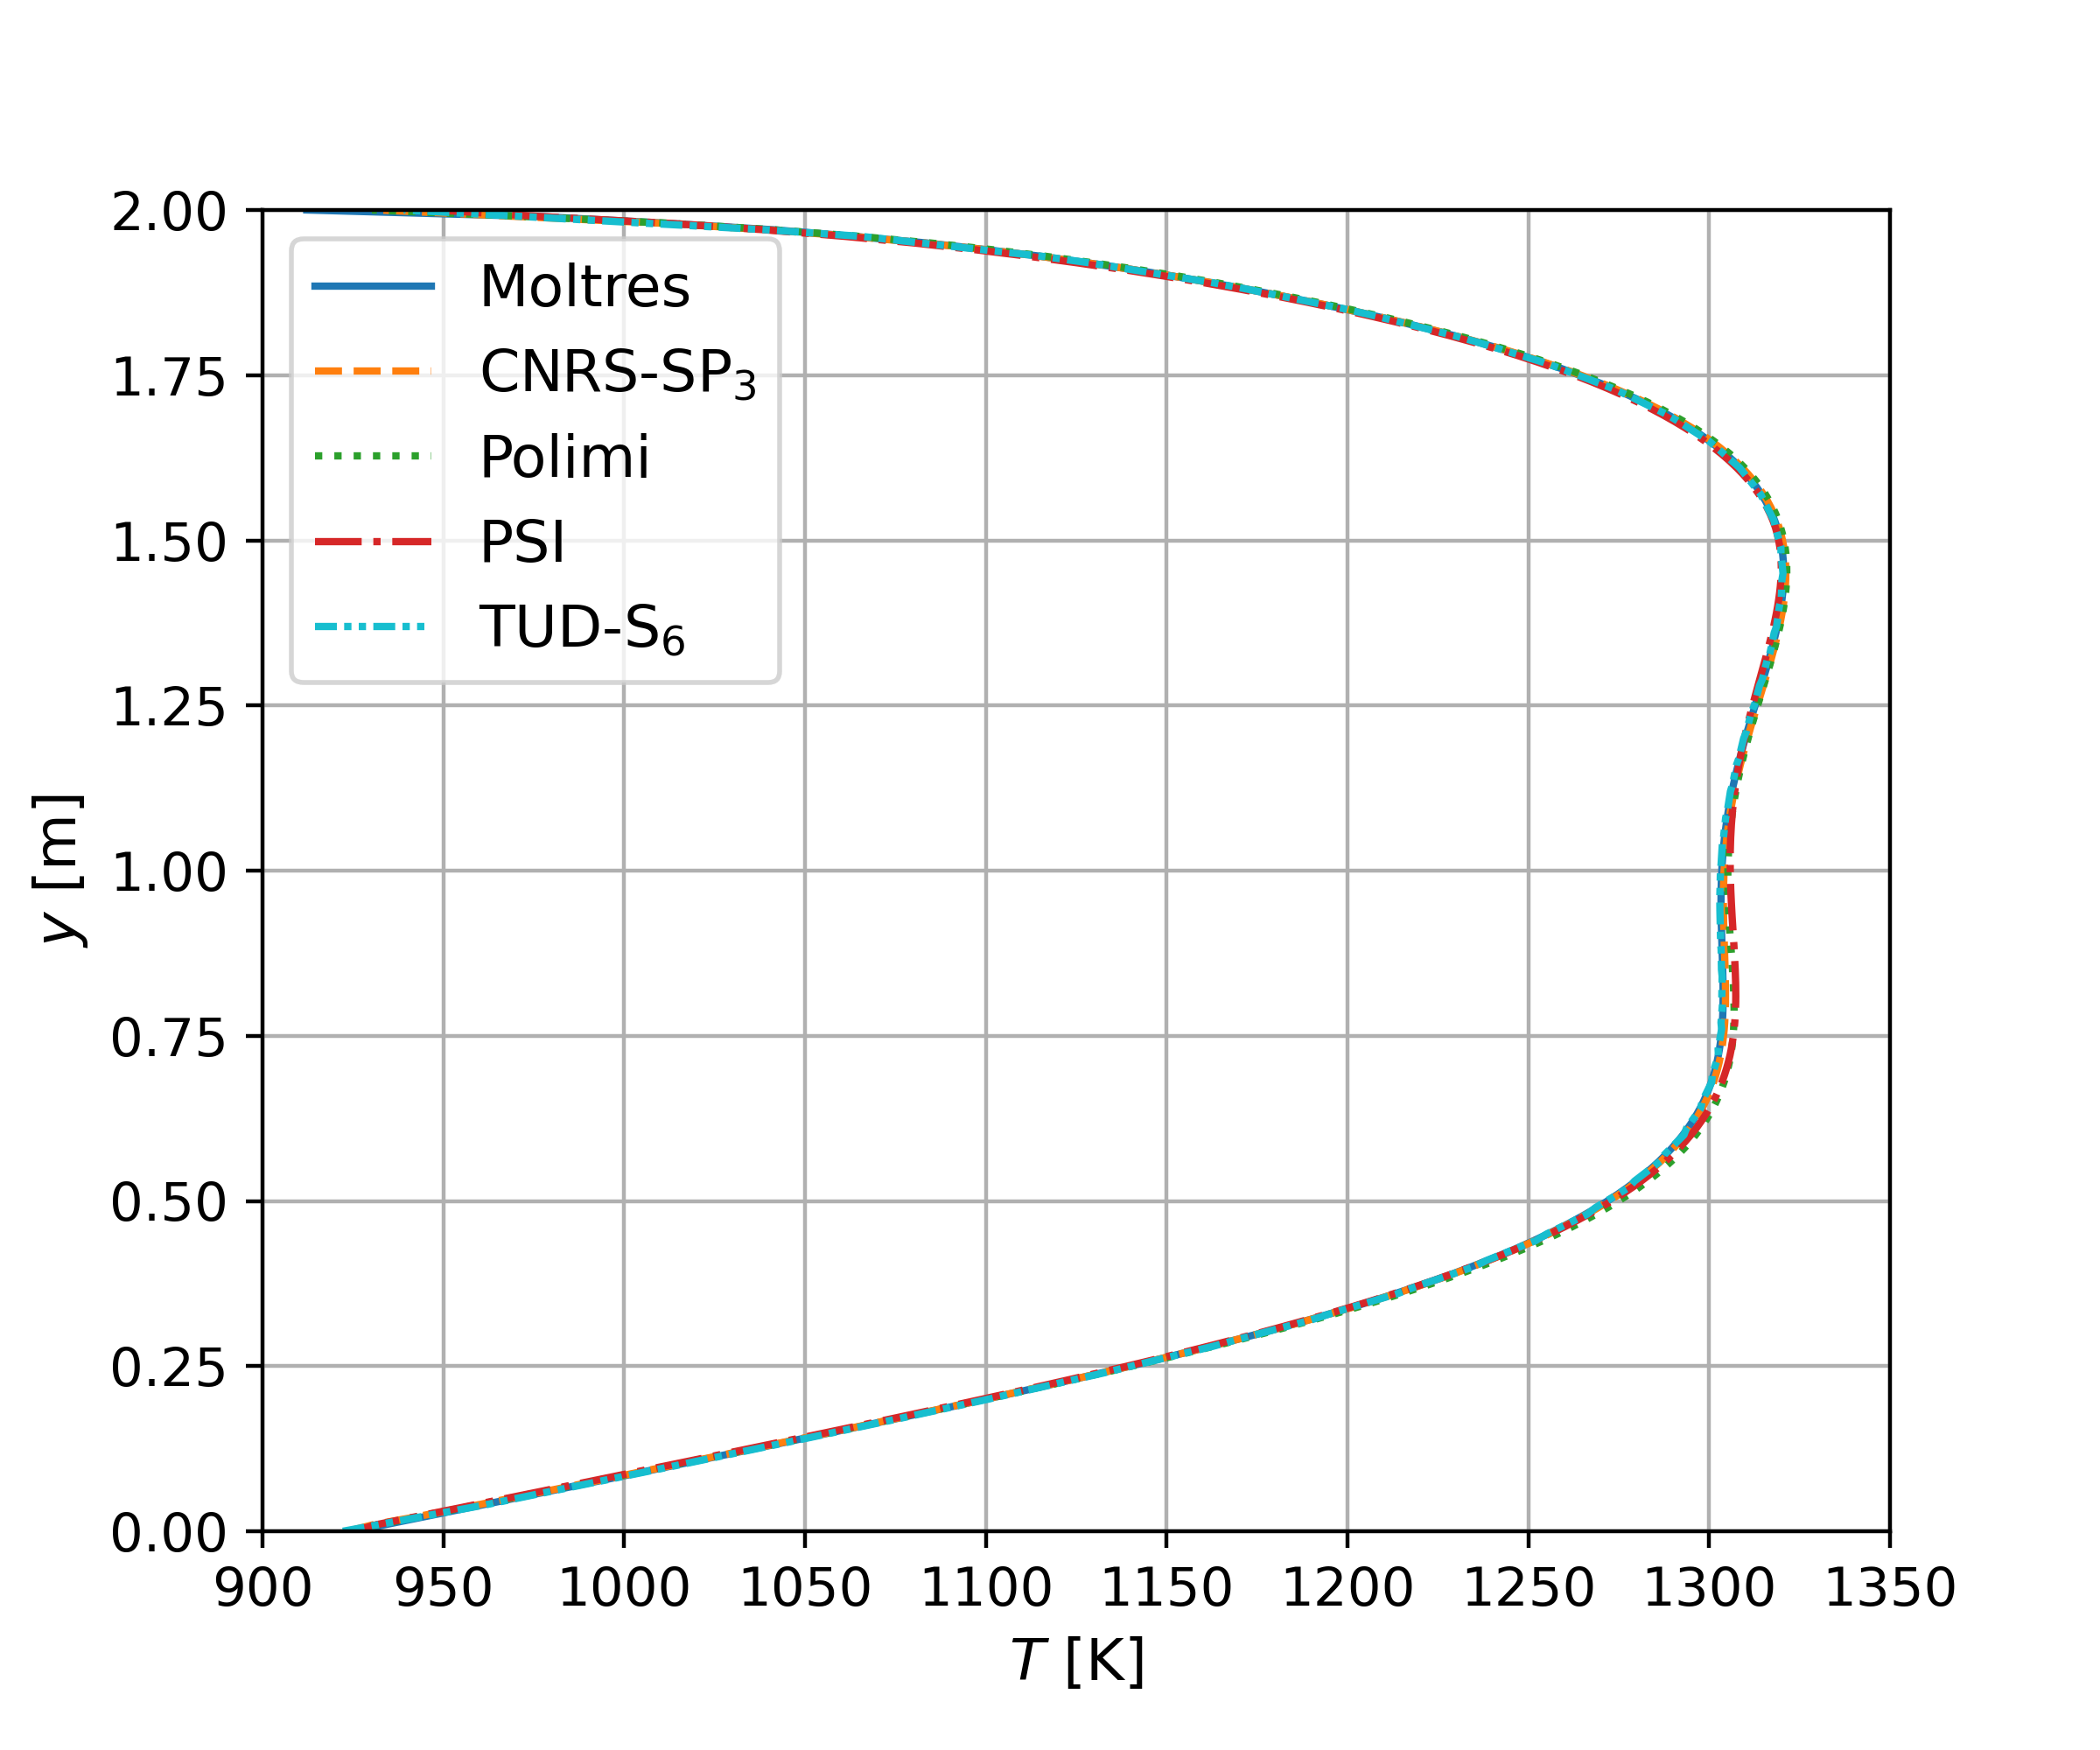
\includegraphics[width=\columnwidth]{0-3-temp-plot}
	  \caption{Step 0.3 \textemdash\ Temperature distribution along BB'.}
	  \label{fig:0.3}
    \end{subfigure}
\end{figure}
%
\FloatBarrier
%
\begin{table}[htb]
	\caption{Discrepancy values from Moltres alongside the average and standard
	deviation of the discrepancy values of the benchmark participants for Phase
	0.}
	\centering
	\small
	\begin{tabular}{l l c S S S}
		\toprule
		\multirow{2}{*}{\textbf{Step}} & \multirow{2}{*}{\textbf{Observable}} & \multirow{2}{*}{\textbf{Centerline}} & {\multirow{2}{*}{\textbf{Moltres [\%]}}} & \multicolumn{2}{c}{\textbf{Benchmark [\%]}} \\
		& & & & {Average} & {SD} \\
		\midrule
		\multirow{4}{*}{0.1} &
		\multirow{2}{*}{$u_x$} & AA' & 0.247 & 0.253 & 0.150 \\
		& & BB' & 0.266 & 0.318 & 0.102 \\
		\cmidrule{2-6}
		& \multirow{2}{*}{$u_y$} & AA' & 0.540 & 0.598 & 0.266 \\
		& & BB' & 0.468 & 0.795 & 0.421 \\
		\midrule
		{0.2} &
		{$\sum^6_g \Sigma_{f,g} \phi_g(\vec{r})$} & AA' & 0.313 & 0.285 & 0.153
		\\
		\midrule
		\multirow{2}{*}{0.3} &
		\multirow{2}{*}{$T$} & AA' & 0.090 & 0.085 & 0.031 \\
		& & BB' & 0.164 & 0.083 & 0.027\\
		\bottomrule
	\end{tabular}
	\label{table:disc0}
\end{table}

\subsubsection{Phase 0 results \& discussion}

Figures \ref{fig:0.1}, \ref{fig:0.2}, and \ref{fig:0.3} show that Moltres
accurately reproduced all three sets of results in Phase 0 for the velocity
field, fission rate density, and temperature. Table
\ref{table:disc0} reports the discrepancy values from Moltres for Phase 0 and
the corresponding average and \gls{SD} of the discrepancy values from
the benchmark participants
\cite{tiberga_results_2020}. Moltres performs very well as most discrepancy
values are either lower than or fall within one \gls{SD} of the benchmark
average discrepancies. The discrepancy value for $T$ along centerline BB' in
Step 0.3 is the only exception, with its value of 0.164\% being larger than
the benchmark average by 3 \gls{SD}.

Figure \ref{fig:0.3} shows that the $T$ distribution from Moltres is almost
identical to the corresponding distributions from CNRS-$SP_3$ and TUD-$S_6$
along most of centerline BB'. However, Figure \ref{fig:0.3-zoom} shows a
significant spread in the $T$ distributions along BB' from all software
packages near the top boundary. At $y = 2.0$ m, Moltres underpredicts the
temperature at 912.3 K compared to the benchmark participants' values which
range between 930.3 K and 948.1 K. This point on the top boundary lies directly downstream of
the velocity boundary condition discontinuity at the top-left corner.
Corner singularities are generally tricky to approximate with
continuous Galerkin methods \cite{kuhlmann_lid-driven_2018}.
The \gls{SUPG} stabilization scheme dampens numerical oscillations by
introducing pointwise artificial thermal diffusivity, which depends strongly on
the inverse of local velocity magnitude \cite{peterson_overview_2018}.
Therefore, while the \gls{SUPG} scheme effectively eliminates
spurious numerical oscillations everywhere else, it provides little damping
along the top boundary due to the relatively large non-zero velocity boundary
condition. On the other hand, the temperature values in the rest of the domain
and the average discrepancies of the other variables show that Moltres can
still accurately reproduce the expected results, and the temperature deviations
along the top boundary do not impact the overall integrity of our results.

\begin{figure}[htb]
	\centering
	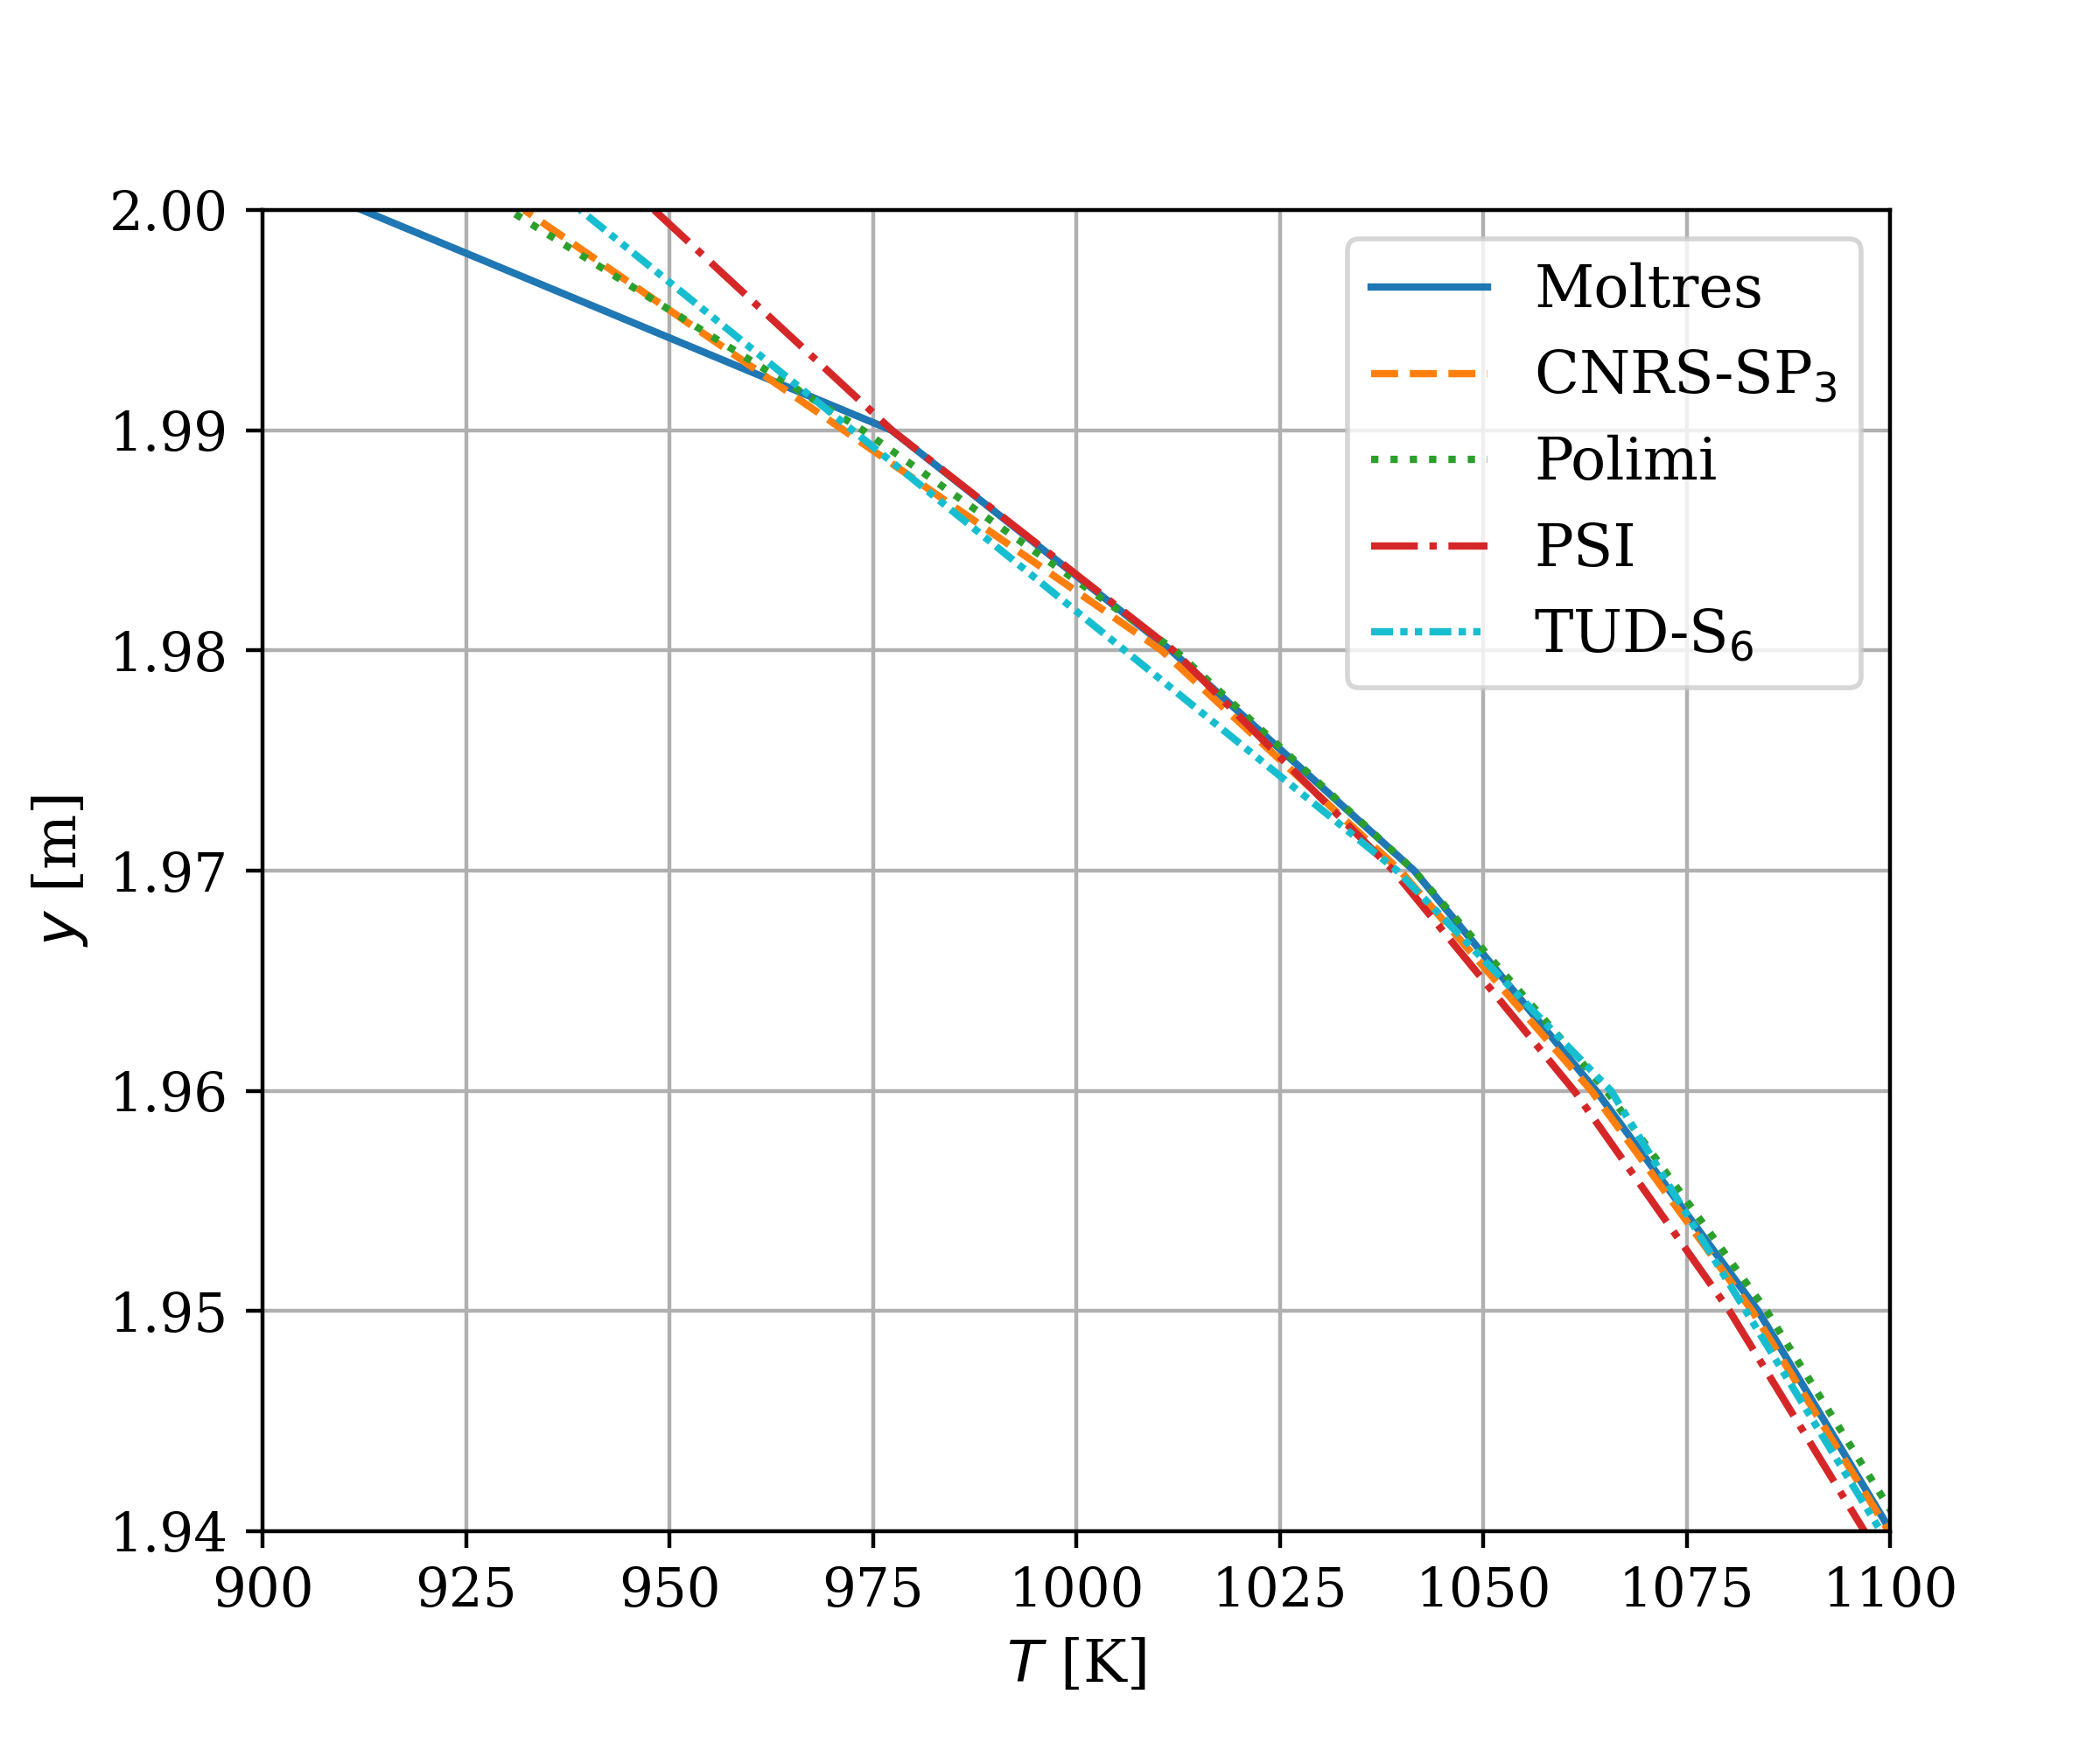
\includegraphics[width=.49\columnwidth]{0-3-temp-plot-zoom}
	\caption{Step 0.3 \textemdash\ Temperature distribution along BB' for y = 1.94 m to
	y = 2.00 m.}
	\label{fig:0.3-zoom}
\end{figure}

Lastly, we observe in table \ref{table:rho} that the reactivity $\rho$ value of
465.6 pcm from Moltres falls well within the range of $\rho$ values from the
benchmark, which range from 353.7 pcm up to 578.1 pcm. Given that Moltres 
adopts the neutron diffusion model, our $\rho$ value agrees closest to the
results from the software packages which also adopt the neutron diffusion model
or theoretically-equivalent models such as the $SP_1$ and $S_2$ neutron
transport models, namely CNRS-$SP_1$, PoliMi, PSI, and TUD-$S_2$.

\begin{table}[htb]
    \caption{Reactivity $\rho$ and change in reactivity
    $\left(\rho_a - \rho_b\right)$ values from Steps 0.2, 1.1,
    1.2, and 1.3. All units are in pcm.}
    \centering
    \small
    \setlength\tabcolsep{2pt}
    \begin{tabular}{l S S S S}
        \toprule
        \multirow{2}{*}{\textbf{Software}} & {\textbf{Step 0.2}} &
        {\textbf{Step 1.1}} & {\textbf{Step 1.2}} & {\textbf{Step 1.3}} \\
        & {$\rho_{s_{0.2}}$}
        & {$\rho_{s_{1.1}} - \rho_{s_{0.2}}$}
        & {$\rho_{s_{1.2}} - \rho_{s_{1.1}}$}
        & {$\rho_{s_{1.3}} - \rho_{s_{0.2}}$} \\
        \midrule
        Moltres     & 465.6 & -62.7 & -1142.2 & -1207.7 \\
        CNRS-$SP_1$ & 411.3 & -62.5 & -1152.0 & -1220.5 \\
        CNRS-$SP_3$ & 353.7 & -62.6 & -1152.7 & -1220.7 \\
        PoliMi      & 421.2 & -62.0 & -1161.0 & -1227.0 \\
        PSI         & 411.7 & -63.0 & -1154.8 & -1219.6 \\
        TUD-$S_2$   & 482.6 & -62.0 & -1145.2 & -1208.5 \\
        TUD-$S_6$   & 578.1 & -60.7 & -1122.0 & -1184.4 \\
        \bottomrule
    \end{tabular}
    \label{table:rho}
\end{table}

\FloatBarrier

\subsubsection{Phase 1 results \& discussion}

Table \ref{table:disc1} shows the discrepancy values from Moltres relative to
the average and \gls{SD} of the benchmark participants for Steps 1.1, 1.2, and
1.3 and the corresponding average discrepancy values from the benchmark
\cite{tiberga_results_2020}. The subsequent subsections discuss the results
for each benchmark step in Phase 1.
%
\begin{table}[htb]
	\caption{Discrepancy values from Moltres alongside the average and standard
	deviation of the discrepancy values of the benchmark participants for Phase
	1.}
	\centering
	\small
	\begin{tabular}{l l c S S S}
		\toprule
		\multirow{2}{*}{\textbf{Step}} & \multirow{2}{*}{\textbf{Observable}} & \multirow{2}{*}{\textbf{Centerline}} & {\multirow{2}{*}{\textbf{Moltres [\%]}}} & \multicolumn{2}{c}{\textbf{Benchmark [\%]}} \\
		& & & & {Average} & {SD} \\
		\midrule
		\multirow{2}{*}{1.1} &
		\multirow{2}{*}{$\sum_i \lambda_i C_i$} & AA' & 0.603 & 0.346 & 0.166
		\\
		& & BB' & 0.327 & 0.294 & 0.153 \\
		\midrule
		\multirow{4}{*}{1.2} &
		\multirow{2}{*}{$T$} & AA' & 0.076 & 0.095 & 0.015 \\
		& & BB' & 0.179 & 0.089 & 0.012 \\
		\cmidrule{2-6}
		& \multirow{2}{*}{\footnotesize $\Delta\left[\sum^6_g \Sigma_{f,g} \phi_g(\vec{r})
		\right]_{s_{1.2}-s_{0.2}}$} & AA' & 1.110 & 1.576 & 0.564 \\
		& & BB' & 1.089 & 1.133 & 0.392 \\
		\midrule
		\multirow{7}{*}{1.3} &
		{$u_x$} & AA' & 0.123 & 0.691 & 0.566 \\
		\cmidrule{2-6}
		& \multirow{2}{*}{$u_y$} & AA' & 0.237 & 0.329 & 0.131 \\
		& & BB' & 0.238 & 0.356 & 0.217 \\
		\cmidrule{2-6}
		& \multirow{2}{*}{$T$} & AA' & 0.064 & 0.057 & 0.023 \\
		& & BB' & 0.070 & 0.080 & 0.024 \\
		\cmidrule{2-6}
		& \multirow{2}{*}{$\sum_i \lambda_i C_i$} & AA' & 1.043 & 0.460 & 0.190
		\\
		& & BB' & 0.462 & 1.194 & 0.178 \\
		\bottomrule
	\end{tabular}
	\label{table:disc1}
\end{table}

\paragraph{Step 1.1: Circulating fuel}

Figure \ref{fig:1.1} shows good qualitative agreement in the delayed neutron
source distribution along BB' among Moltres and the benchmark participants.
From Table \ref{table:disc1}, Moltres reports discrepancies of 0.603\% and
0.327\% along the centerlines AA' and BB', respectively. Both values are
within two and one \gls{SD}, respectively, of the average discrepancies of the
benchmark participants (0.346\% and 0.294\%).
In Table \ref{table:rho}, we observe that the change in
$\rho$ relative to Step 0.2 is $-62.7$ pcm for Moltres, and this value is
consistent with the $-63.0$ to $-62.0$ pcm range that most of the benchmark
participants' values fall in.
%
\begin{figure}[htb]
	\centering
    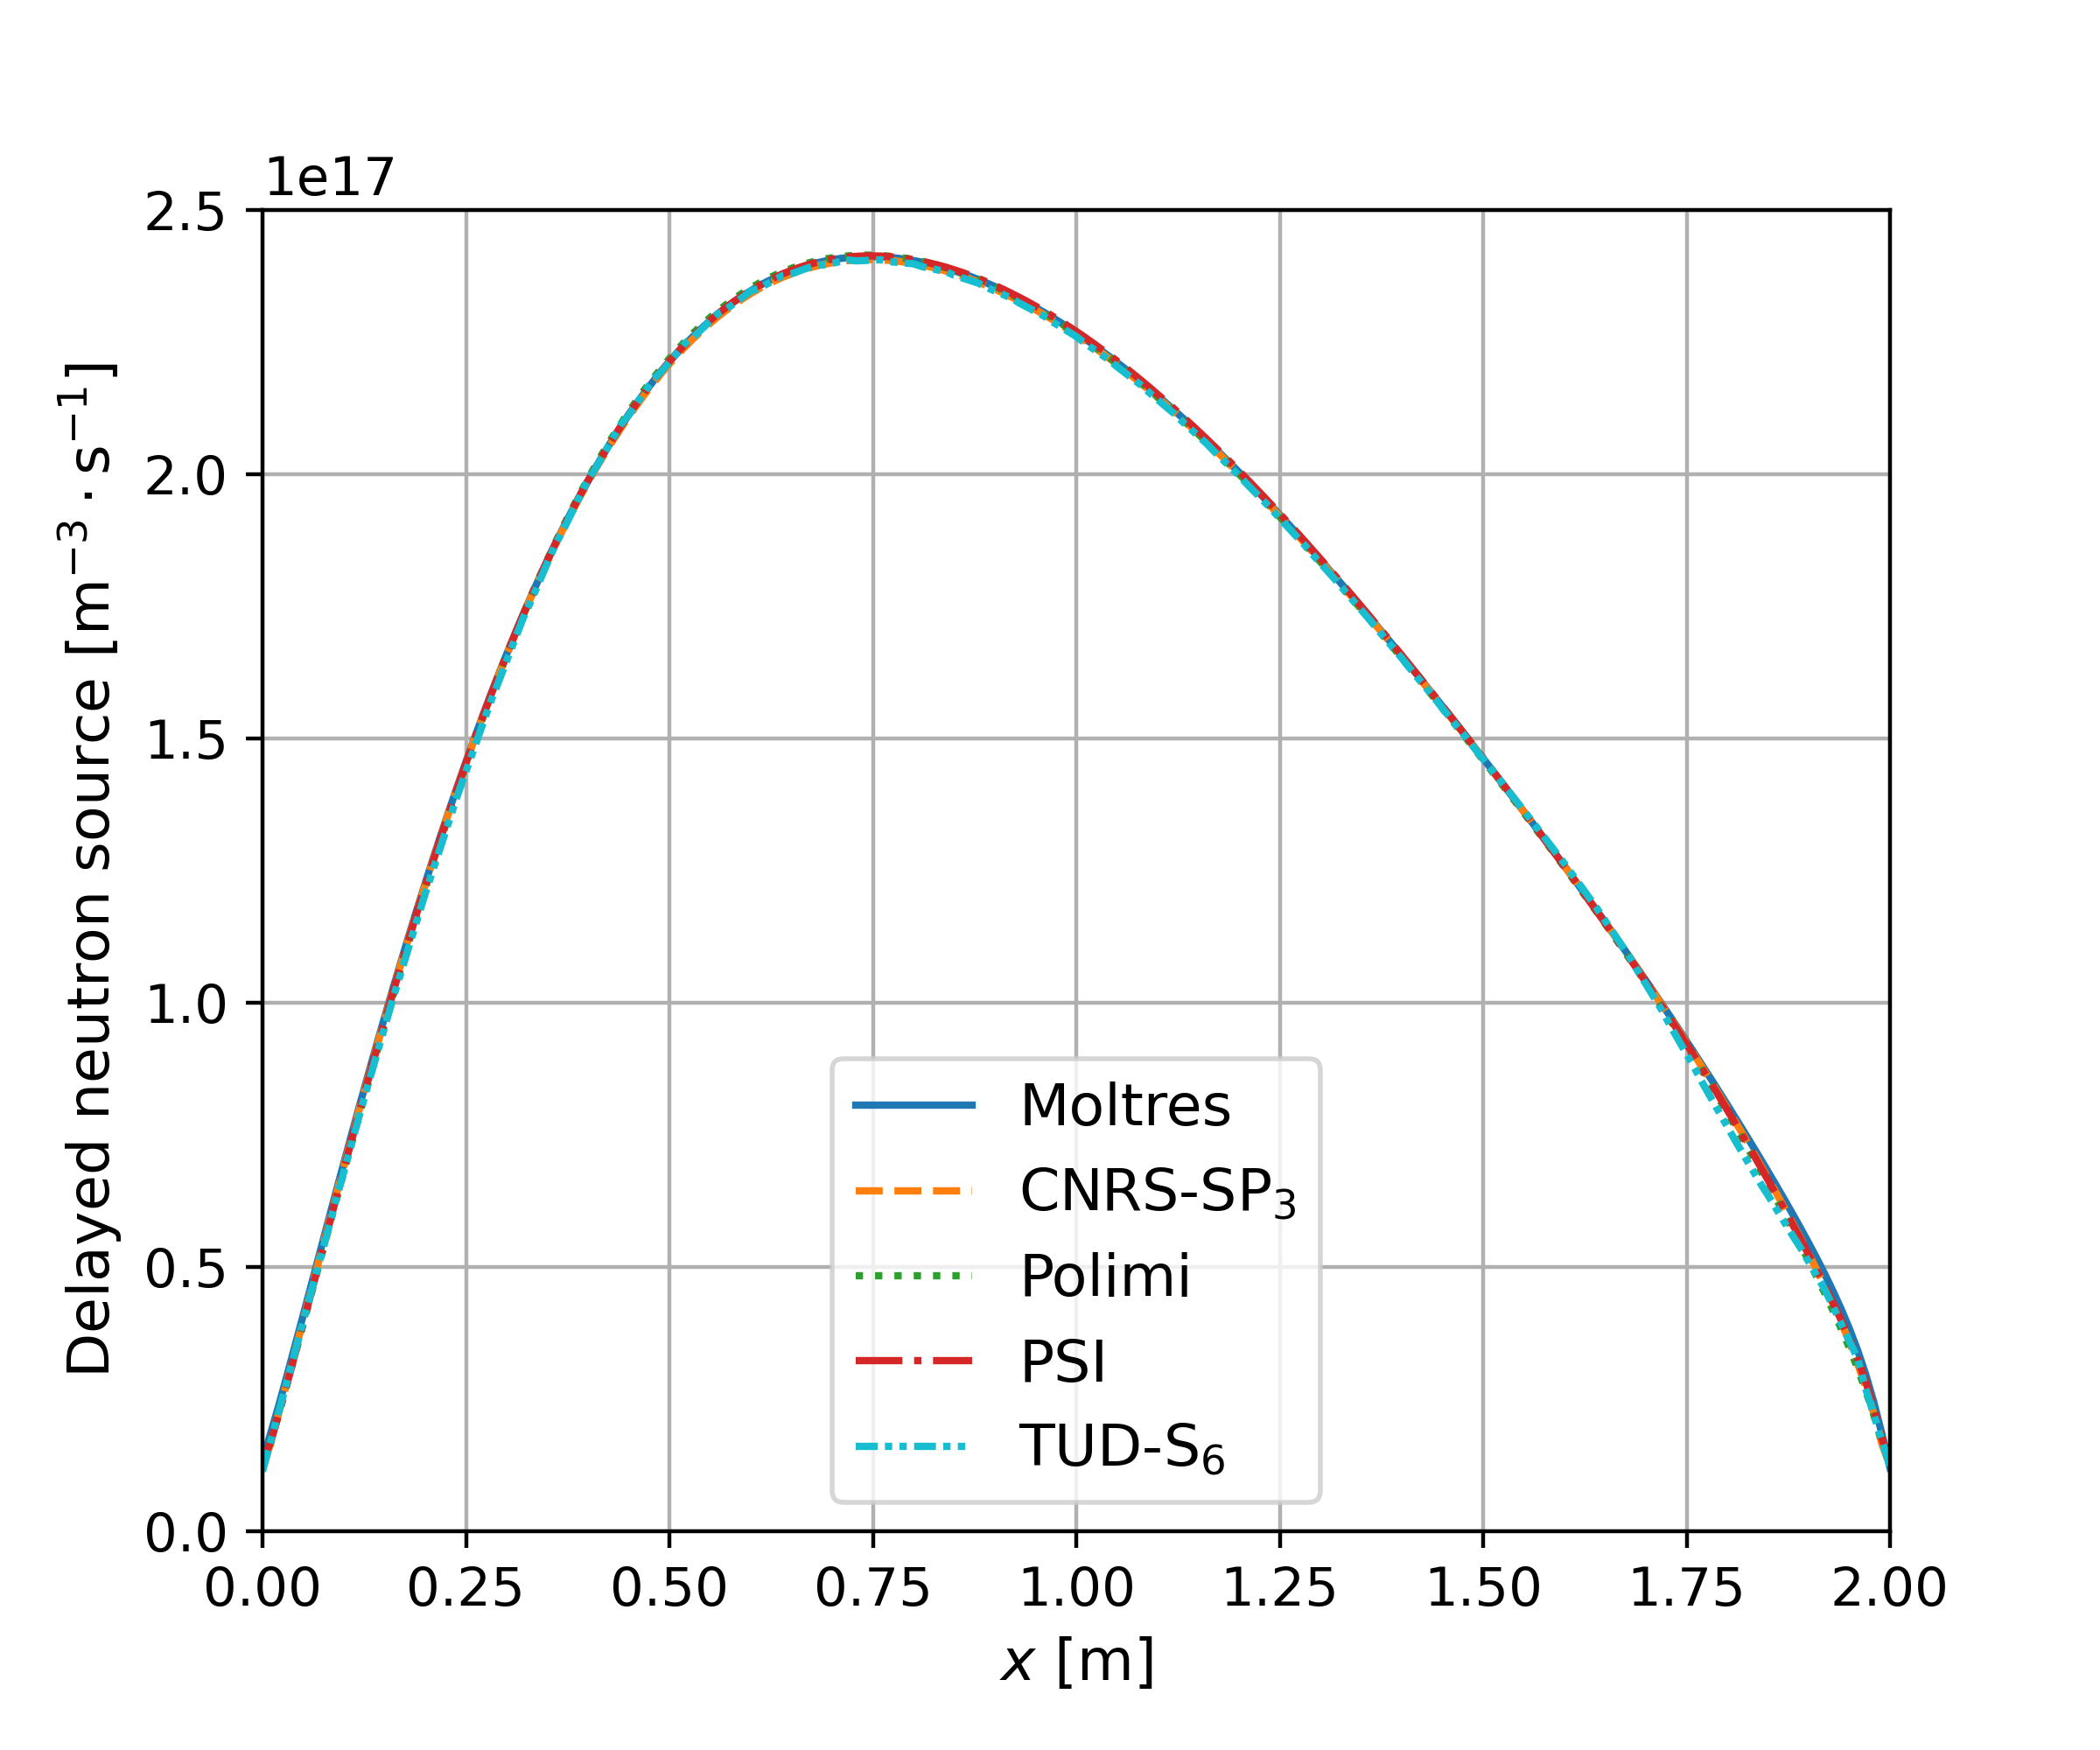
\includegraphics[width=.49\columnwidth]{1-1-dnp-x-plot}
    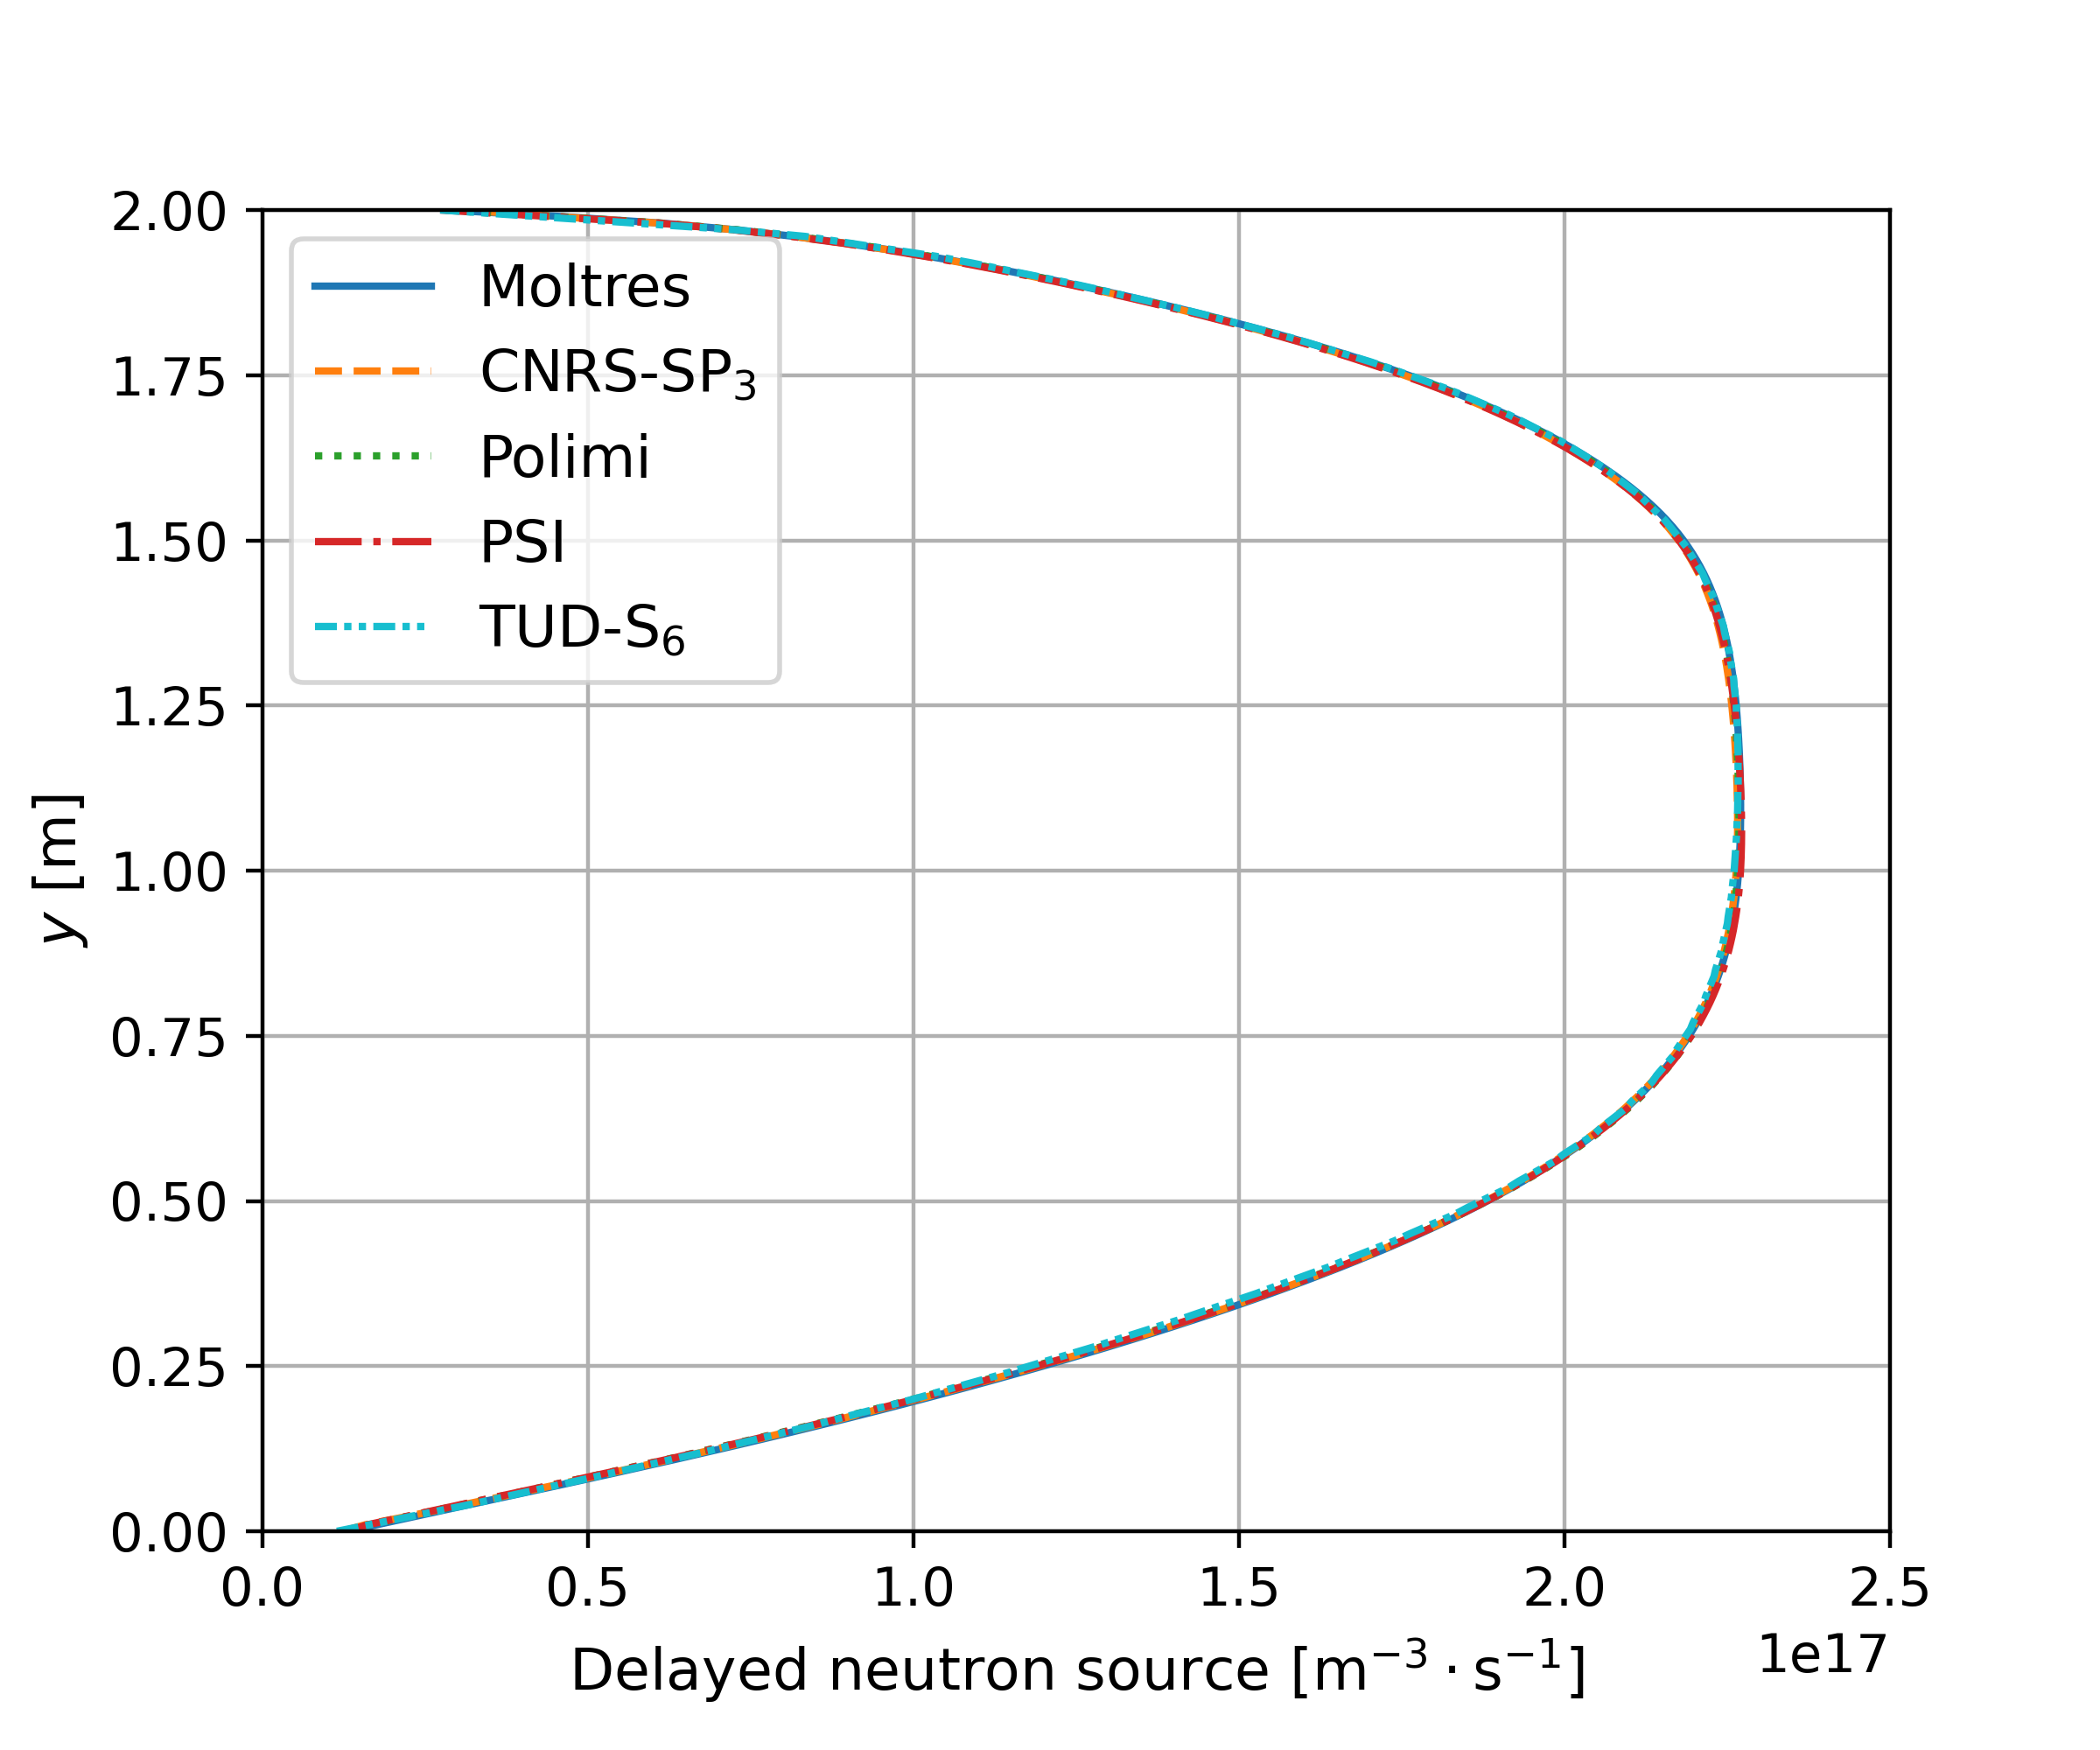
\includegraphics[width=.49\columnwidth]{1-1-dnp-y-plot}
	\caption{Step 1.1 \textemdash\ Delayed neutron source along AA' (top) and BB'
	(bottom).}
	\label{fig:1.1}
\end{figure}
%
\begin{figure}[htb]
	\centering
	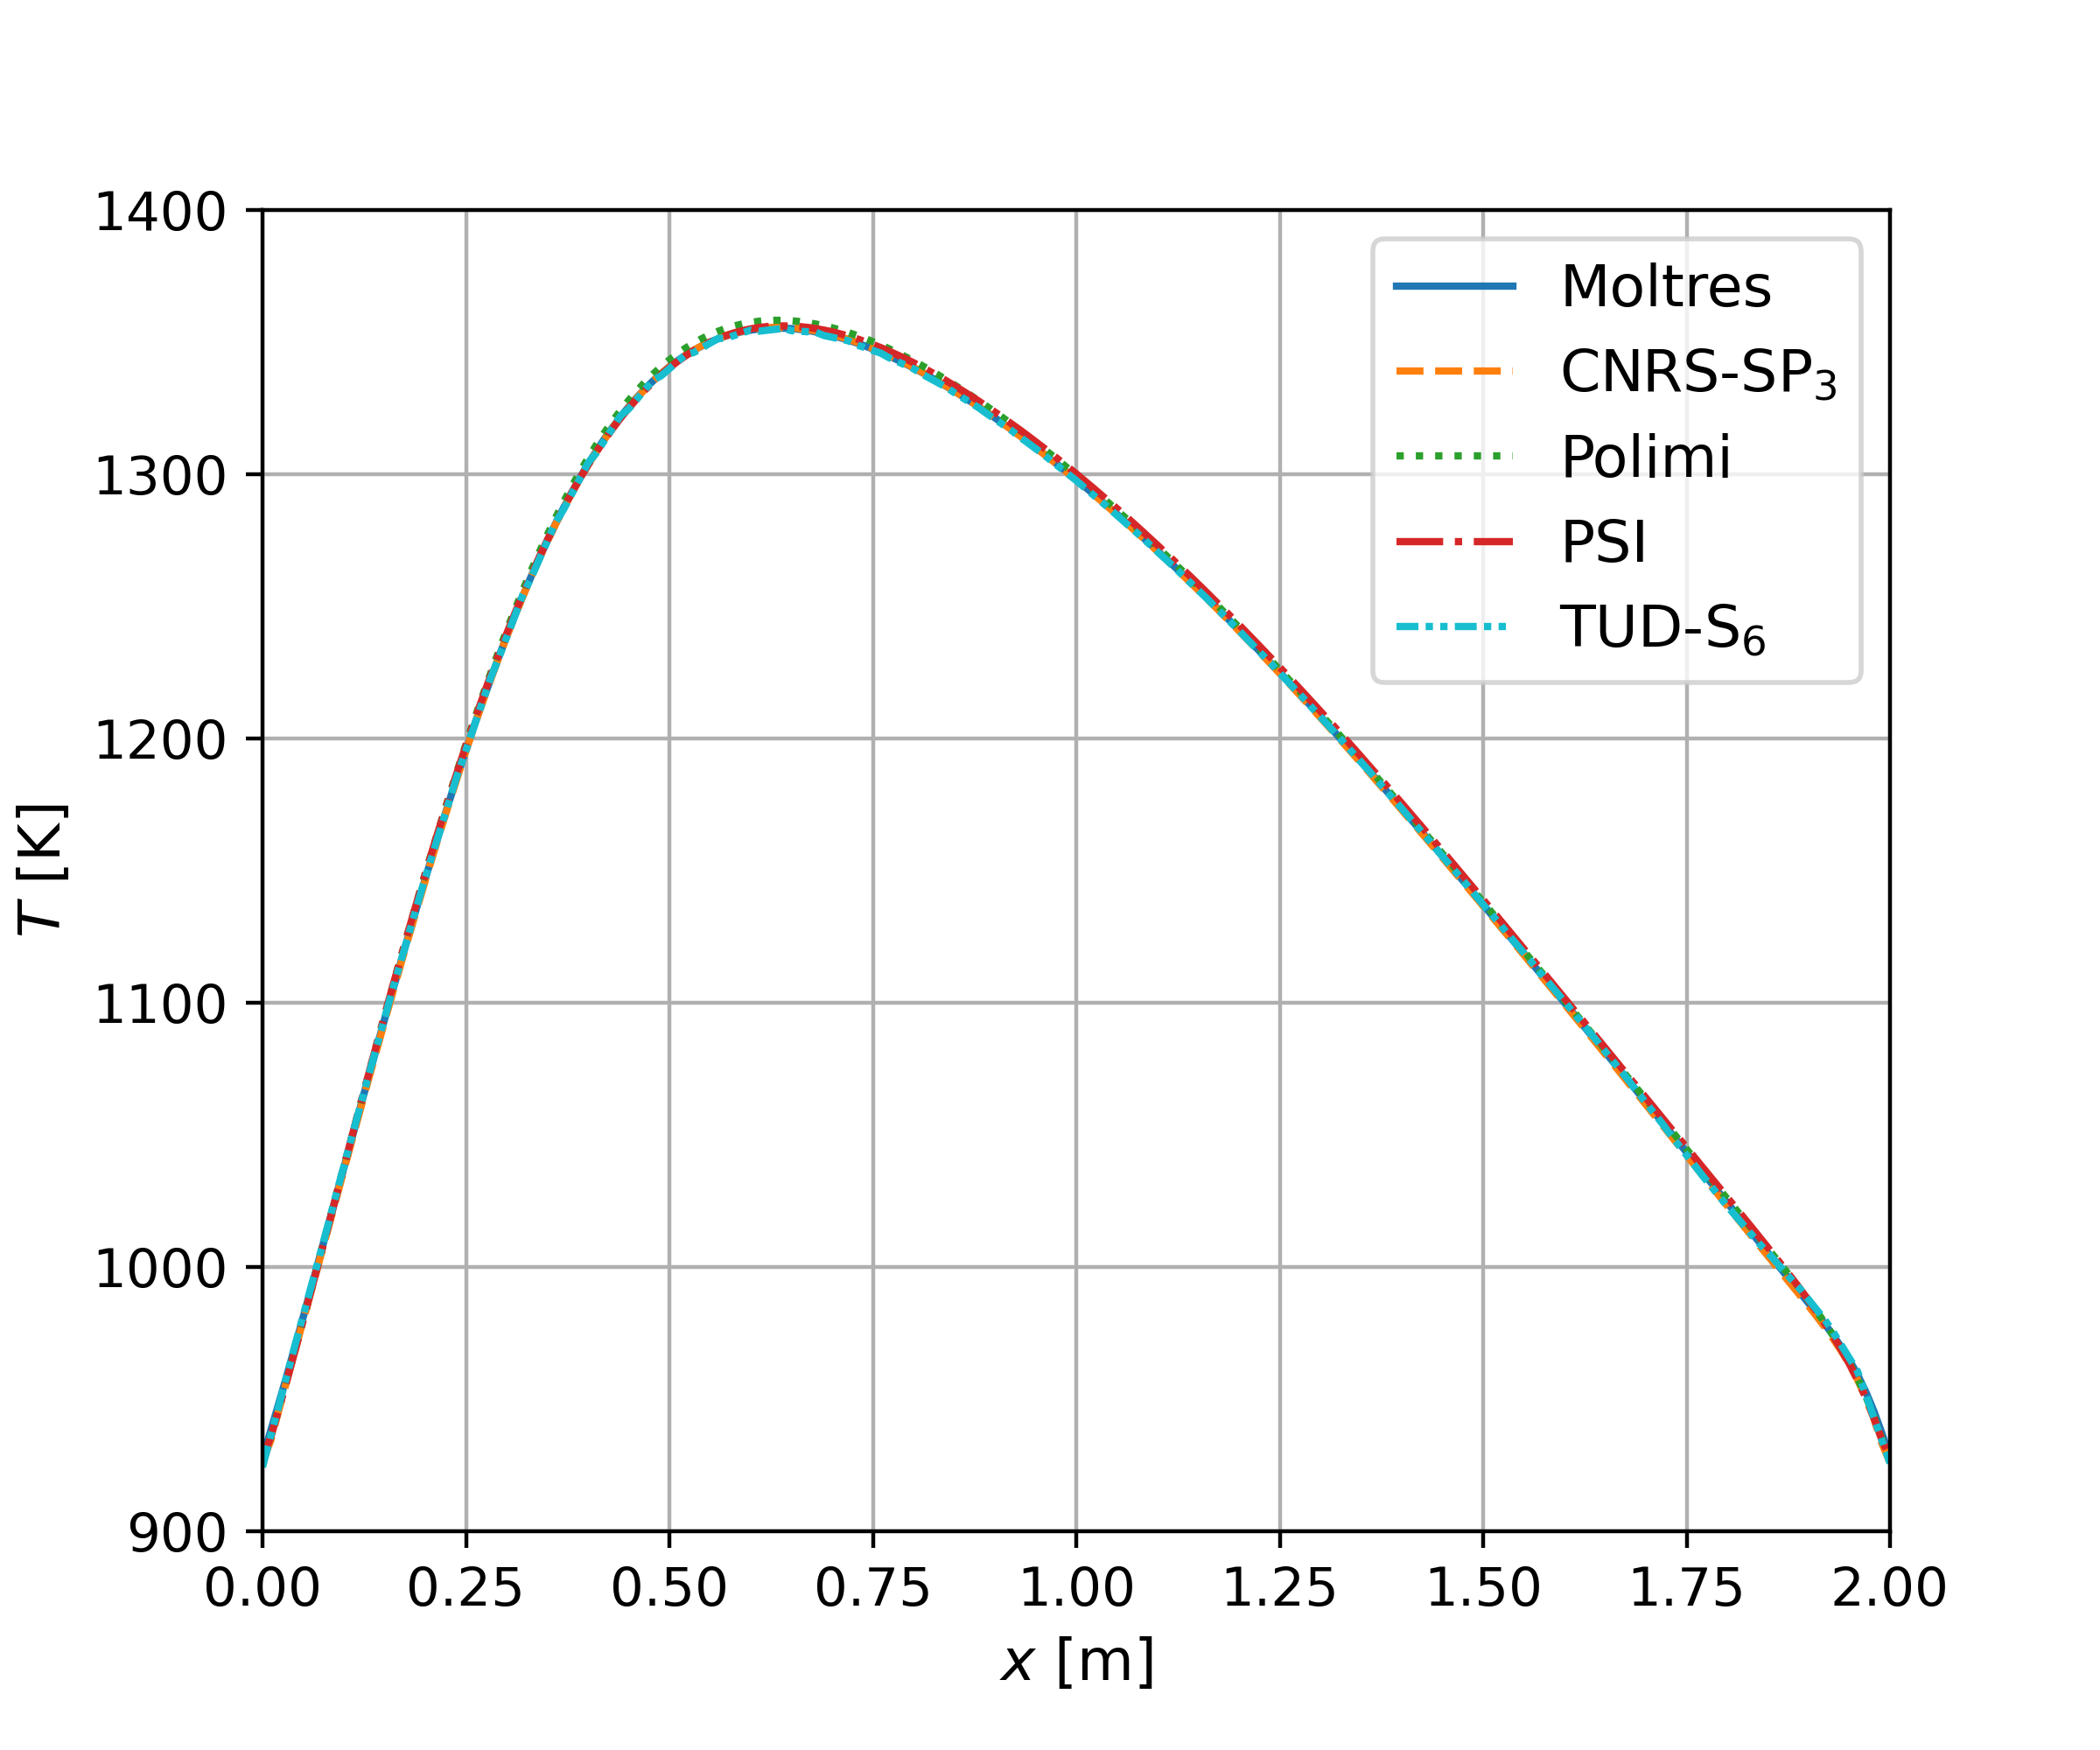
\includegraphics[width=.49\columnwidth]{1-2-temp-plot}
	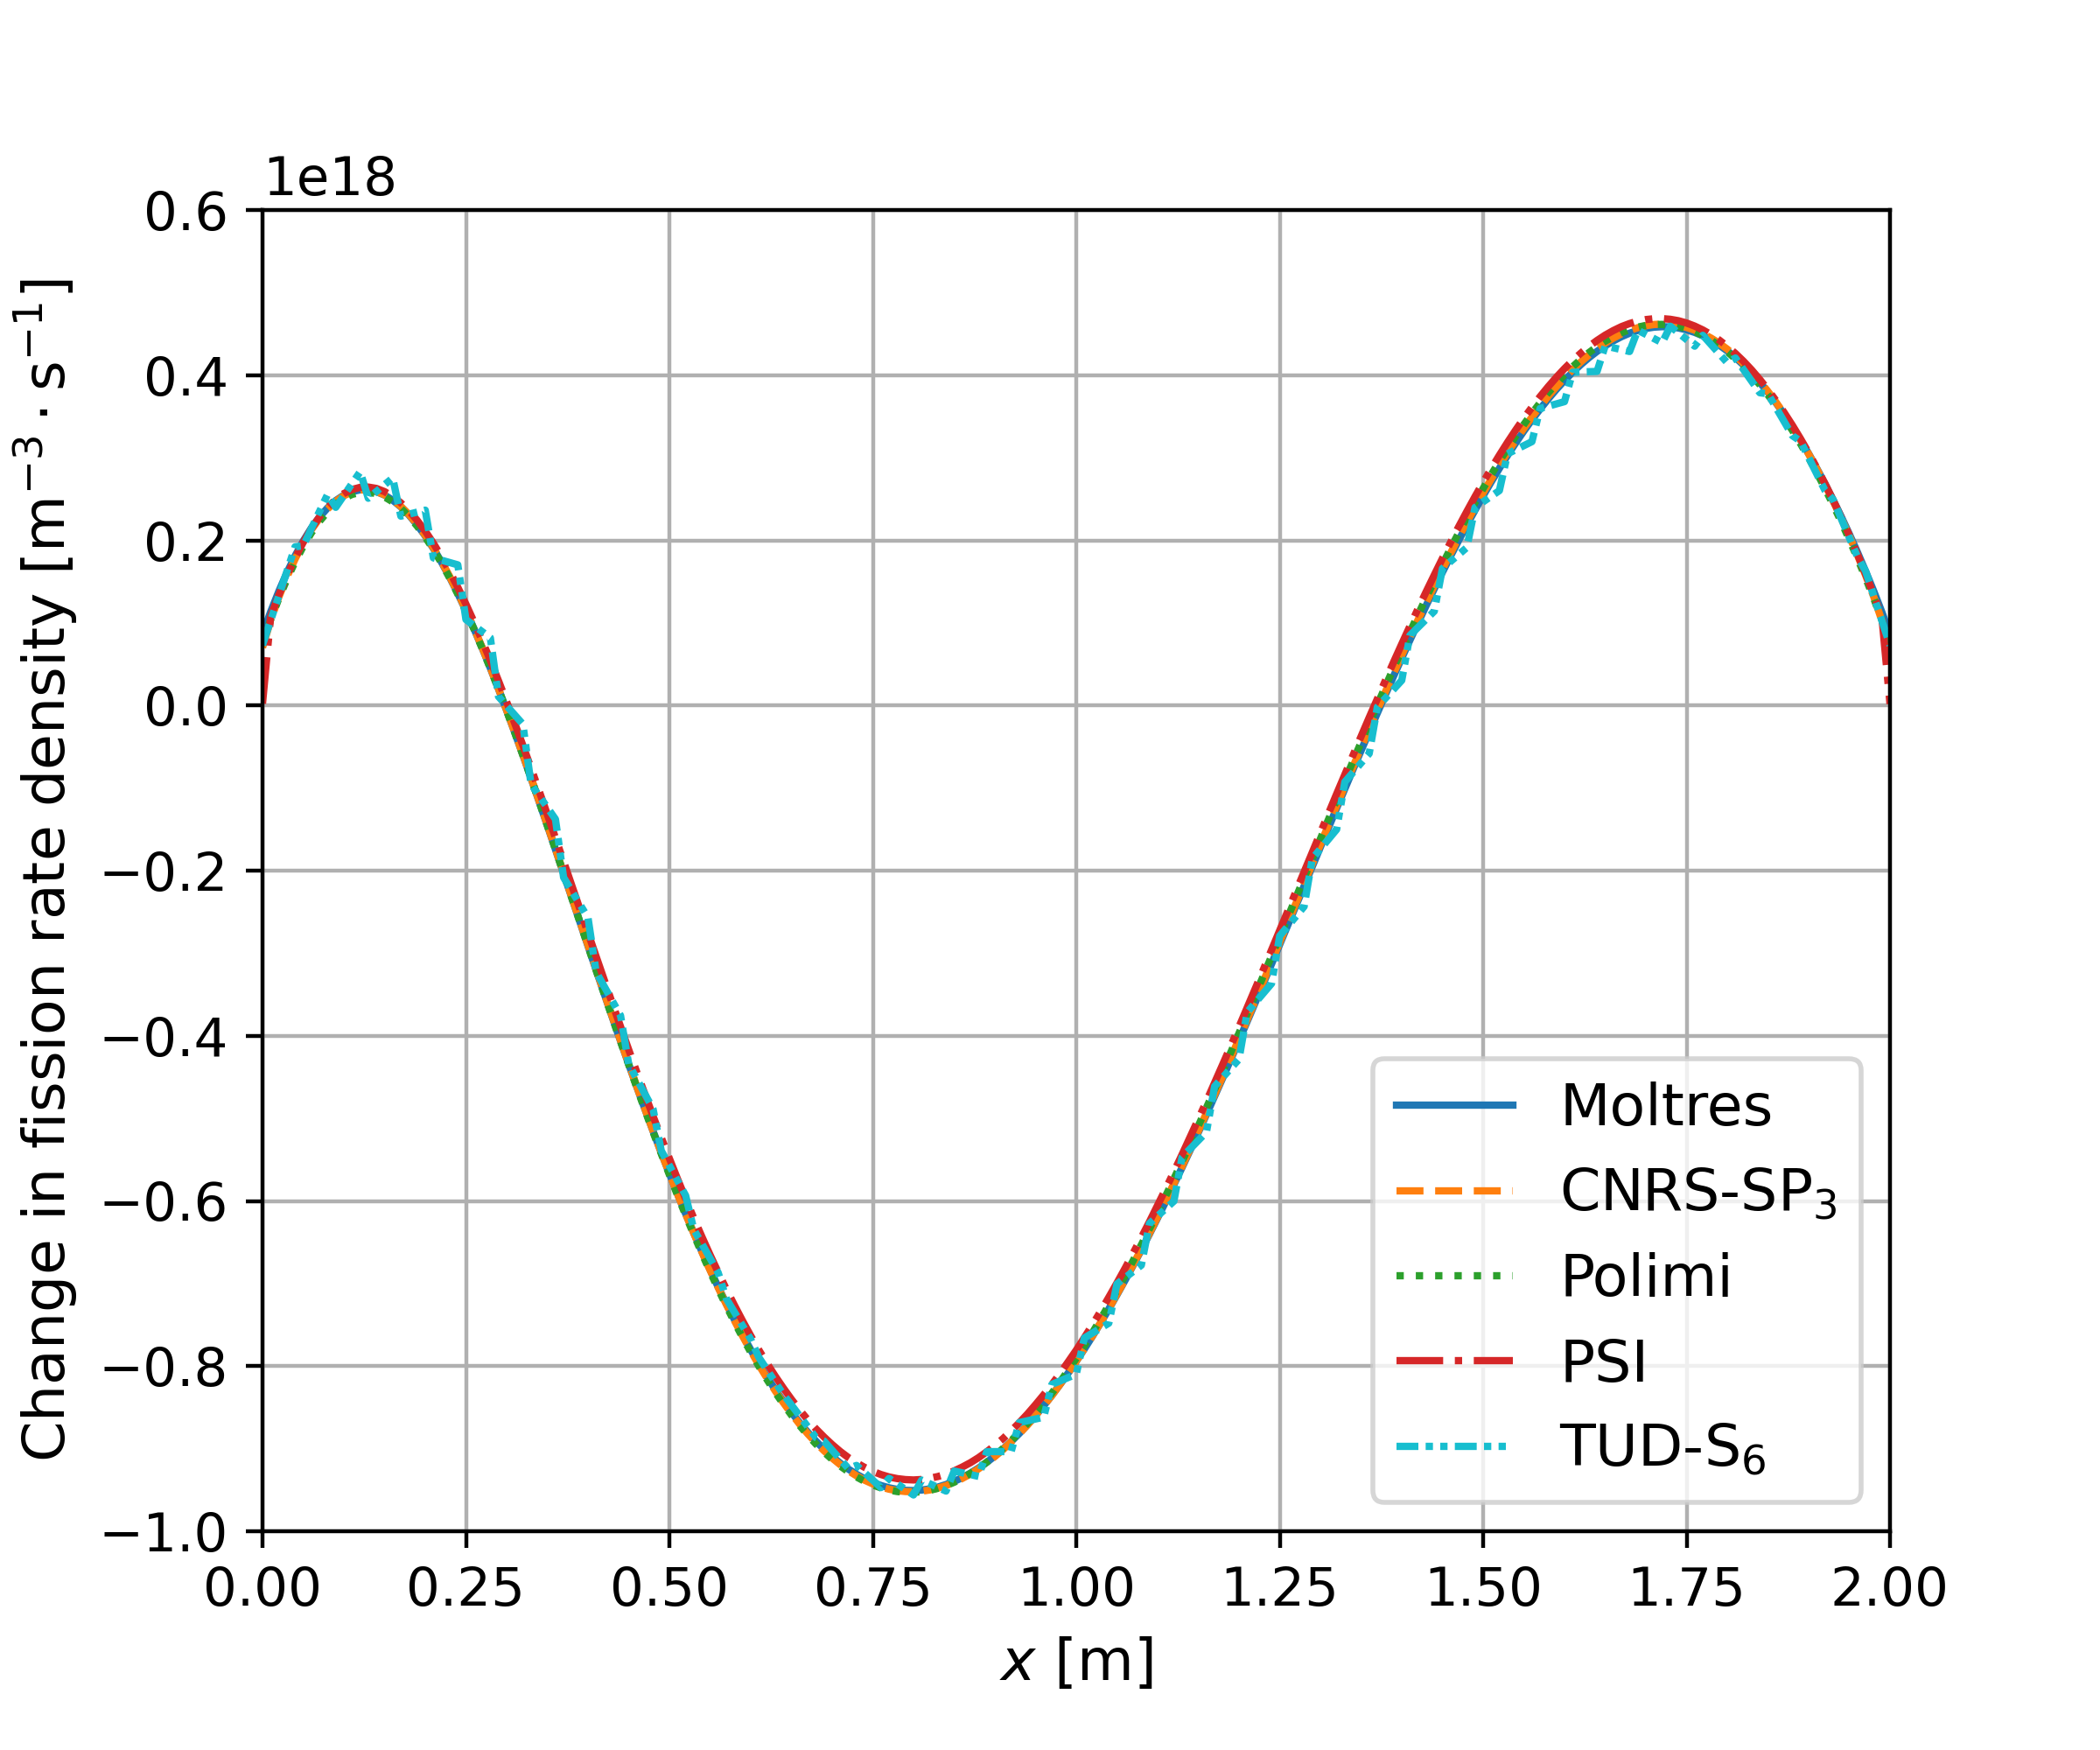
\includegraphics[width=.49\columnwidth]{1-2-fiss-plot}
	\caption{Step 1.2 \textemdash\ Temperature distribution and change in fission rate
	density along AA'.}
	\label{fig:1.2}
\end{figure}

\FloatBarrier

\paragraph{Step 1.2: Power coupling}

Figure \ref{fig:1.2} shows the temperature distribution and the change in
fission rate density along AA' from Step 1.2. Similar to Step 0.3, the
temperature distribution from Moltres agrees closest with CNRS-$SP_3$ and
TUD-$S_2$. Table \ref{table:disc1} reports the same trends we observed in Phase
0; the average discrepancy in temperature along BB' from Moltres for Step 1.2
is marginally higher than the benchmark, while the average discrepancy in the
fission rate density is within one \gls{SD} range to the benchmark average.
From Table \ref{table:rho}, Moltres also reports a change in $\rho$
relative to Step 1.1 of $-1142.2$ pcm, which
falls within the range of reported benchmark participants' values.

\paragraph{Step 1.3: Buoyancy}

Figure \ref{fig:1.3} shows the vertical velocity component, temperature, and
delayed neutron source distributions along AA'.
Moltres reproduces the correct trend in all three physical
observables. Step 1.3 has a relatively slower buoyancy-driven flow profile with
no forced flow from the top boundary. Consequently, there are no temperature
deviations near the top boundary, and we observe in Table \ref{table:disc1} that
the average discrepancy value of 0.070\% for the temperature distribution along
BB' is in much closer agreement to the benchmark value of 0.080\% compared to
the corresponding temperature discrepancy values for Step 0.3 and 1.2.

Table \ref{table:rho} shows that the change in $\rho$ from
Moltres (-1207.7 pcm) falls within the range of reported benchmark values and
matches the software from TUD-$S_2$ (-1208.5 pcm) the closest. This observation is likely
due to the similar solvers (diffusion and $S_2$ neutronics models) and
methods of solution (finite element method on uniform meshes) employed by our
respective software.
%
\begin{figure}[htb]
	\centering
	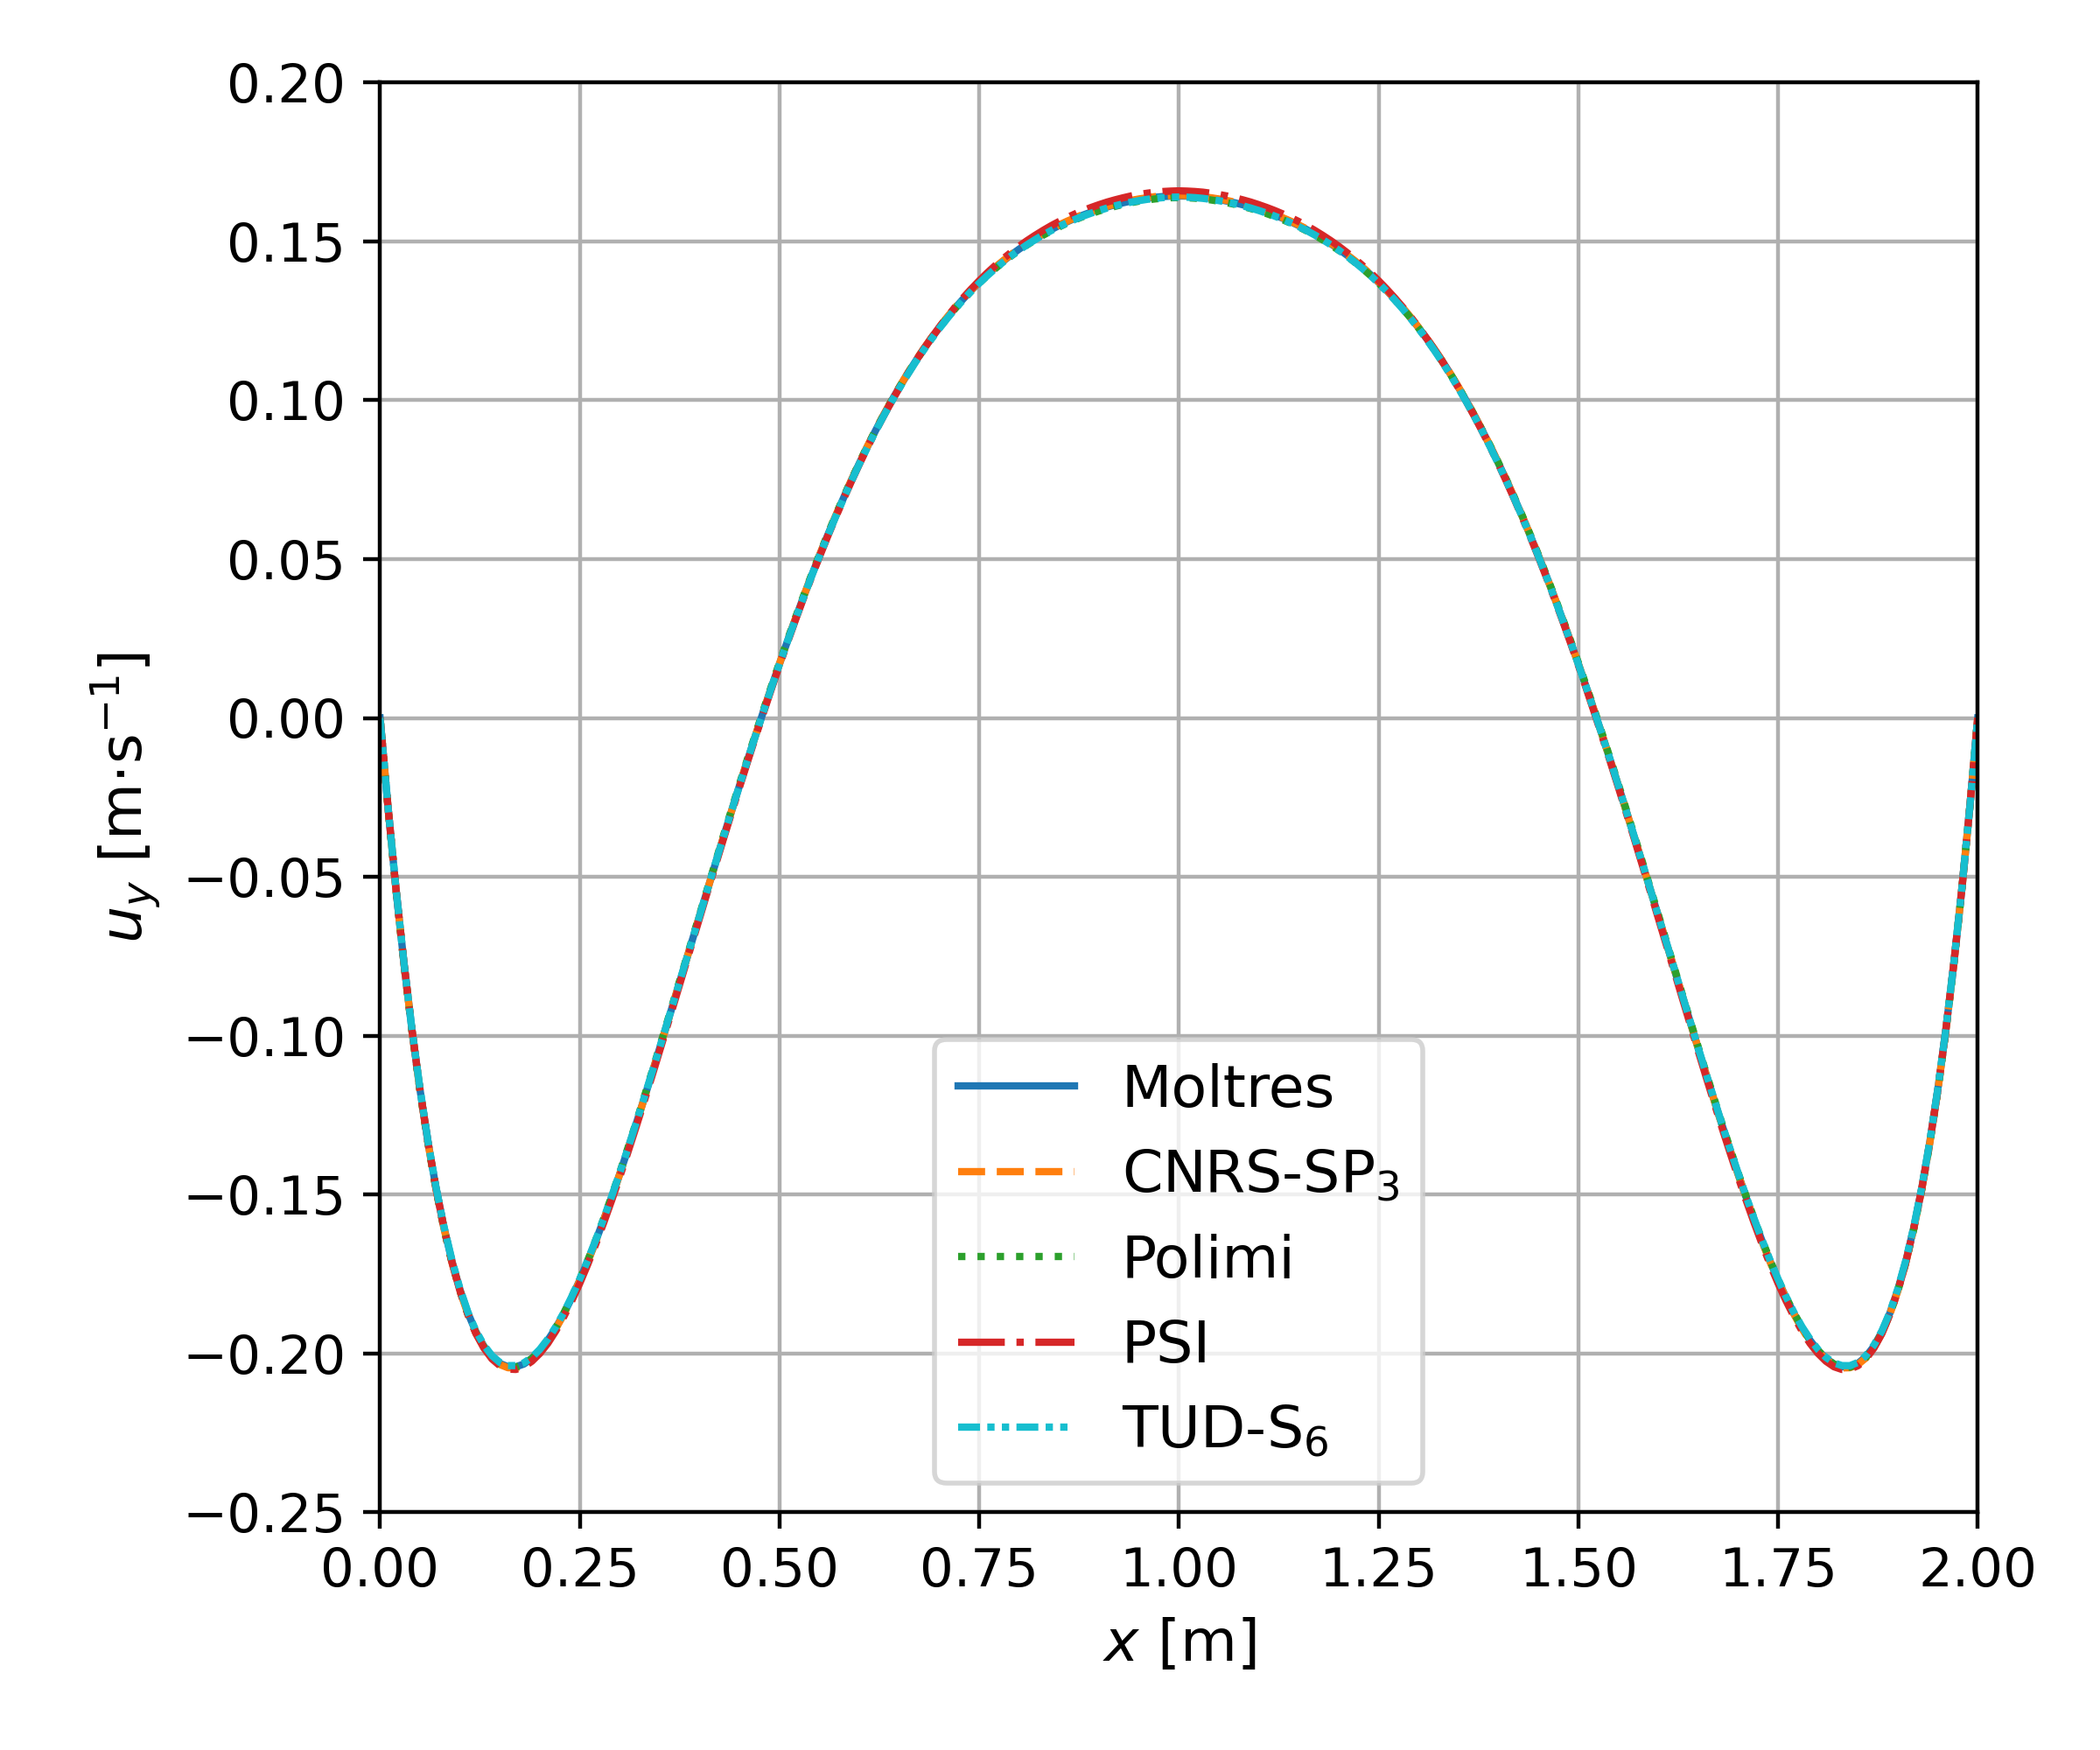
\includegraphics[width=.49\columnwidth]{1-3-vel-plot}
	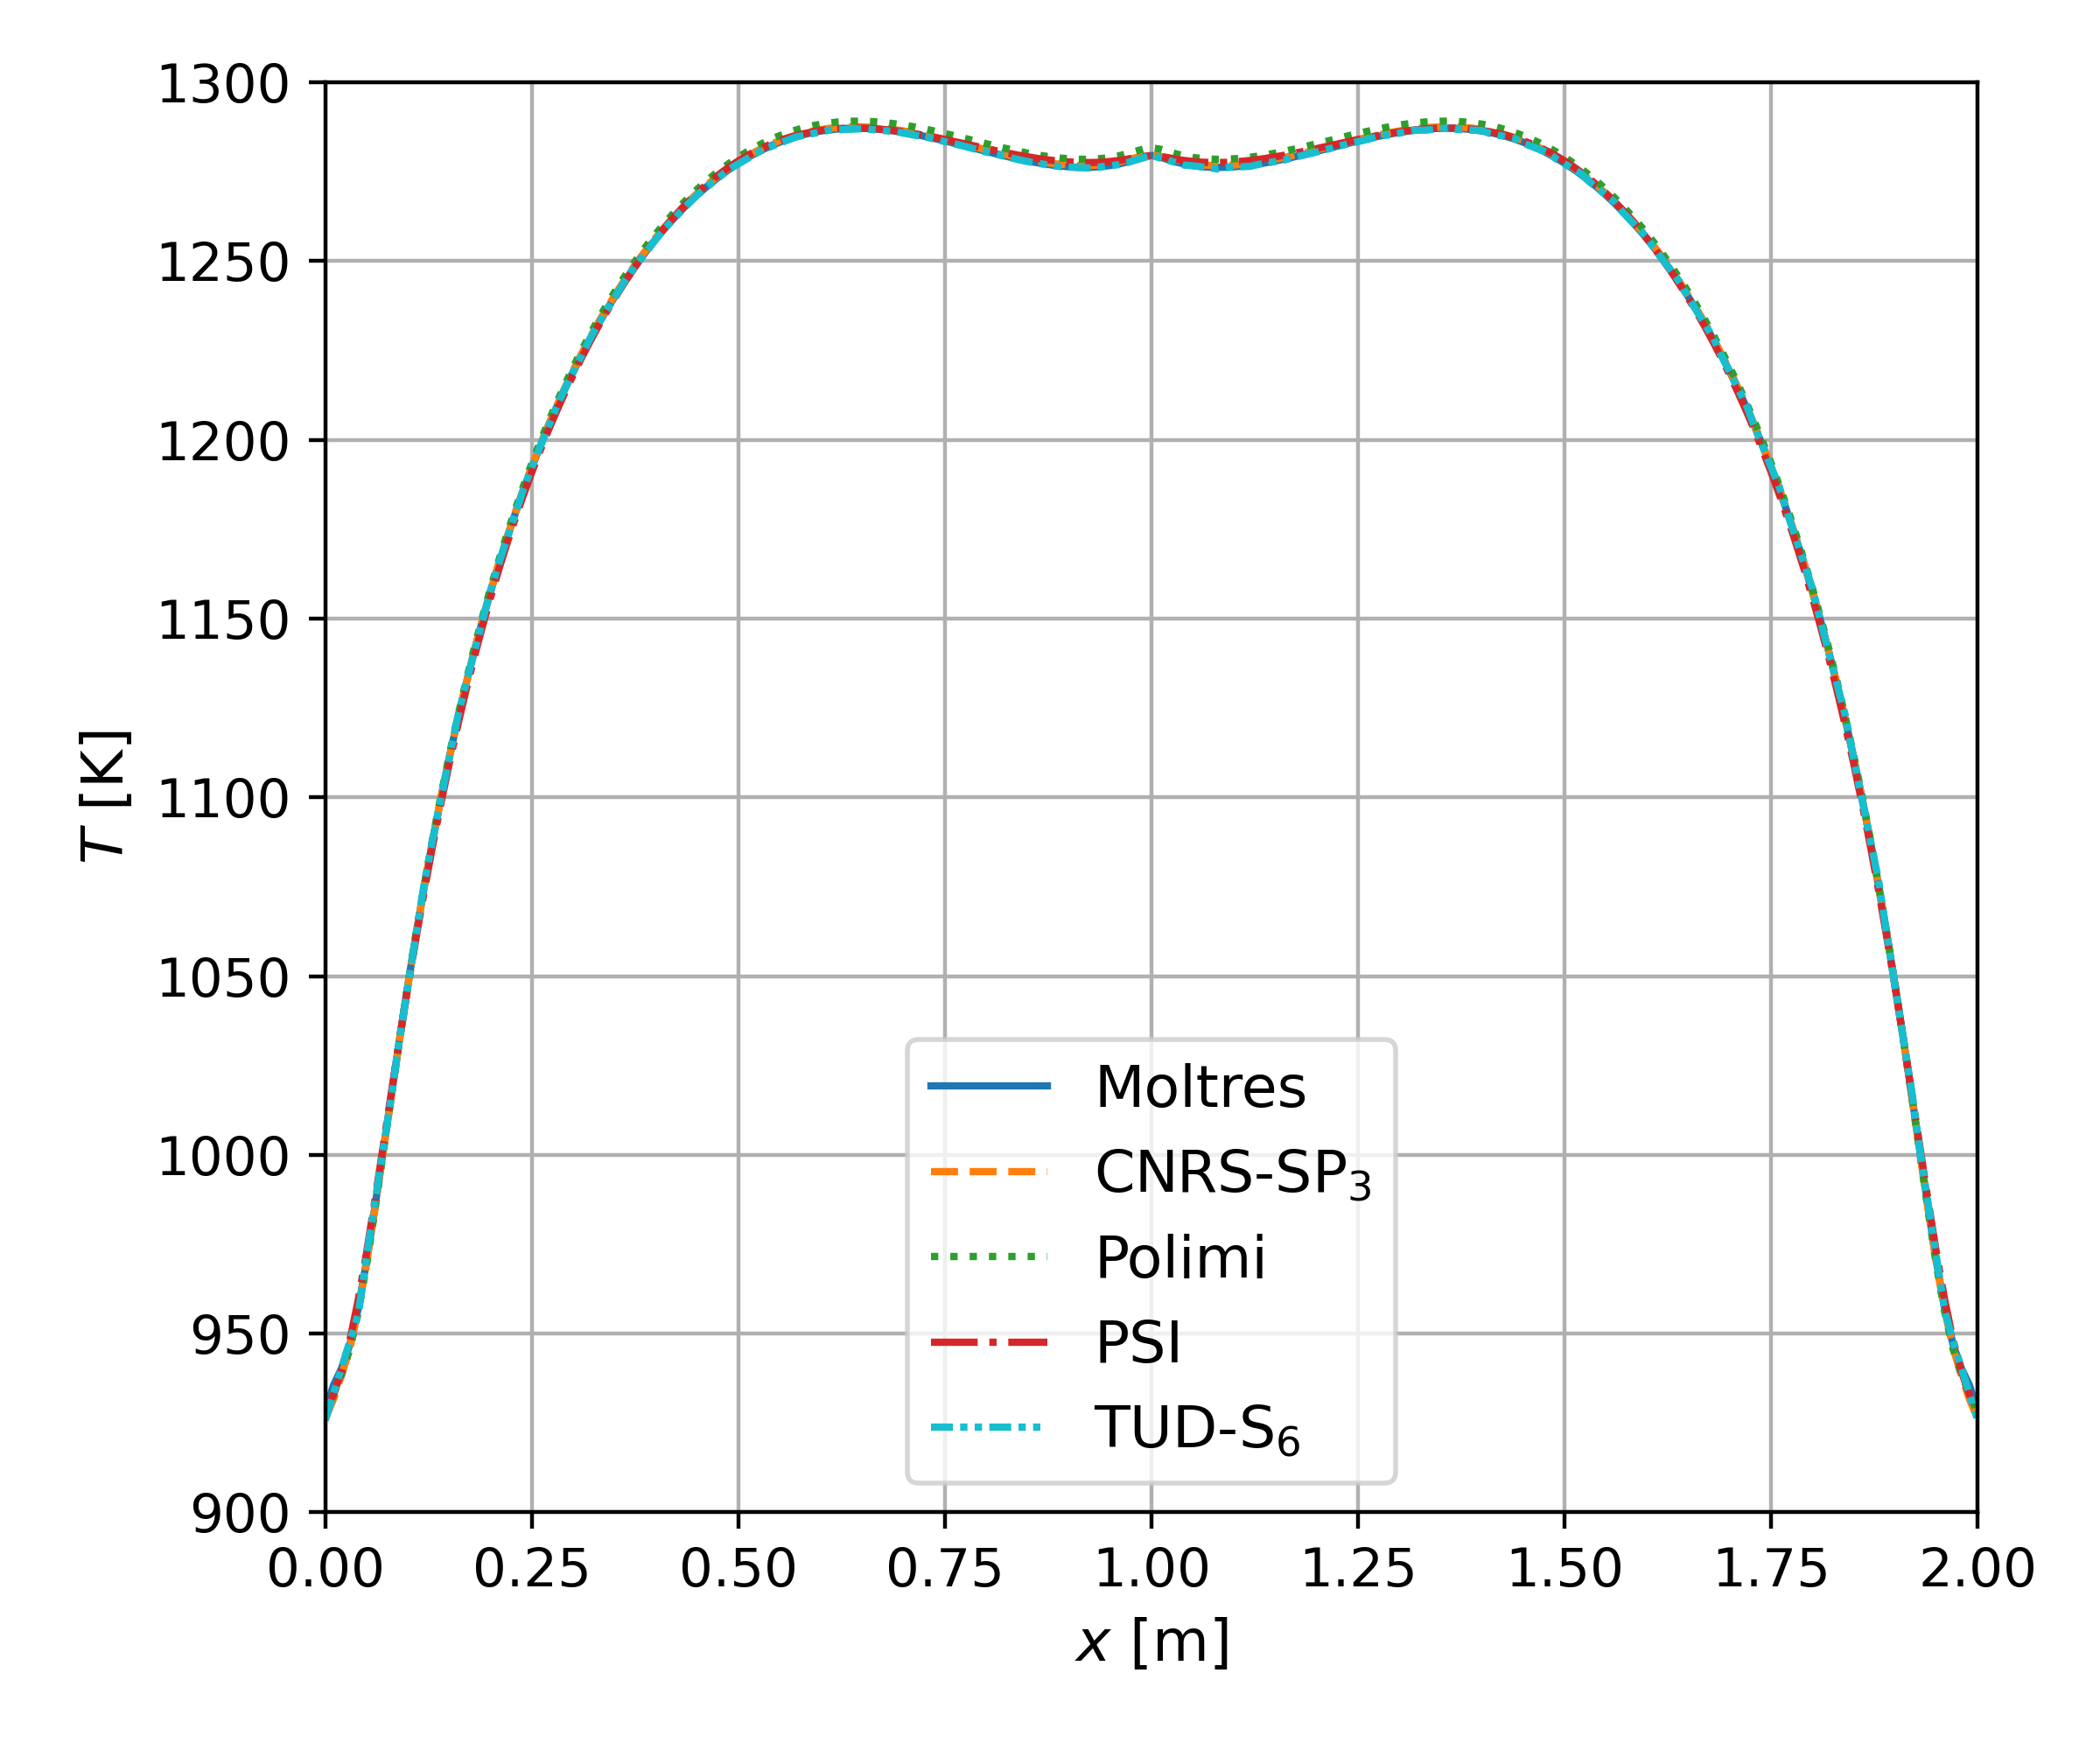
\includegraphics[width=.49\columnwidth]{1-3-temp-plot}
	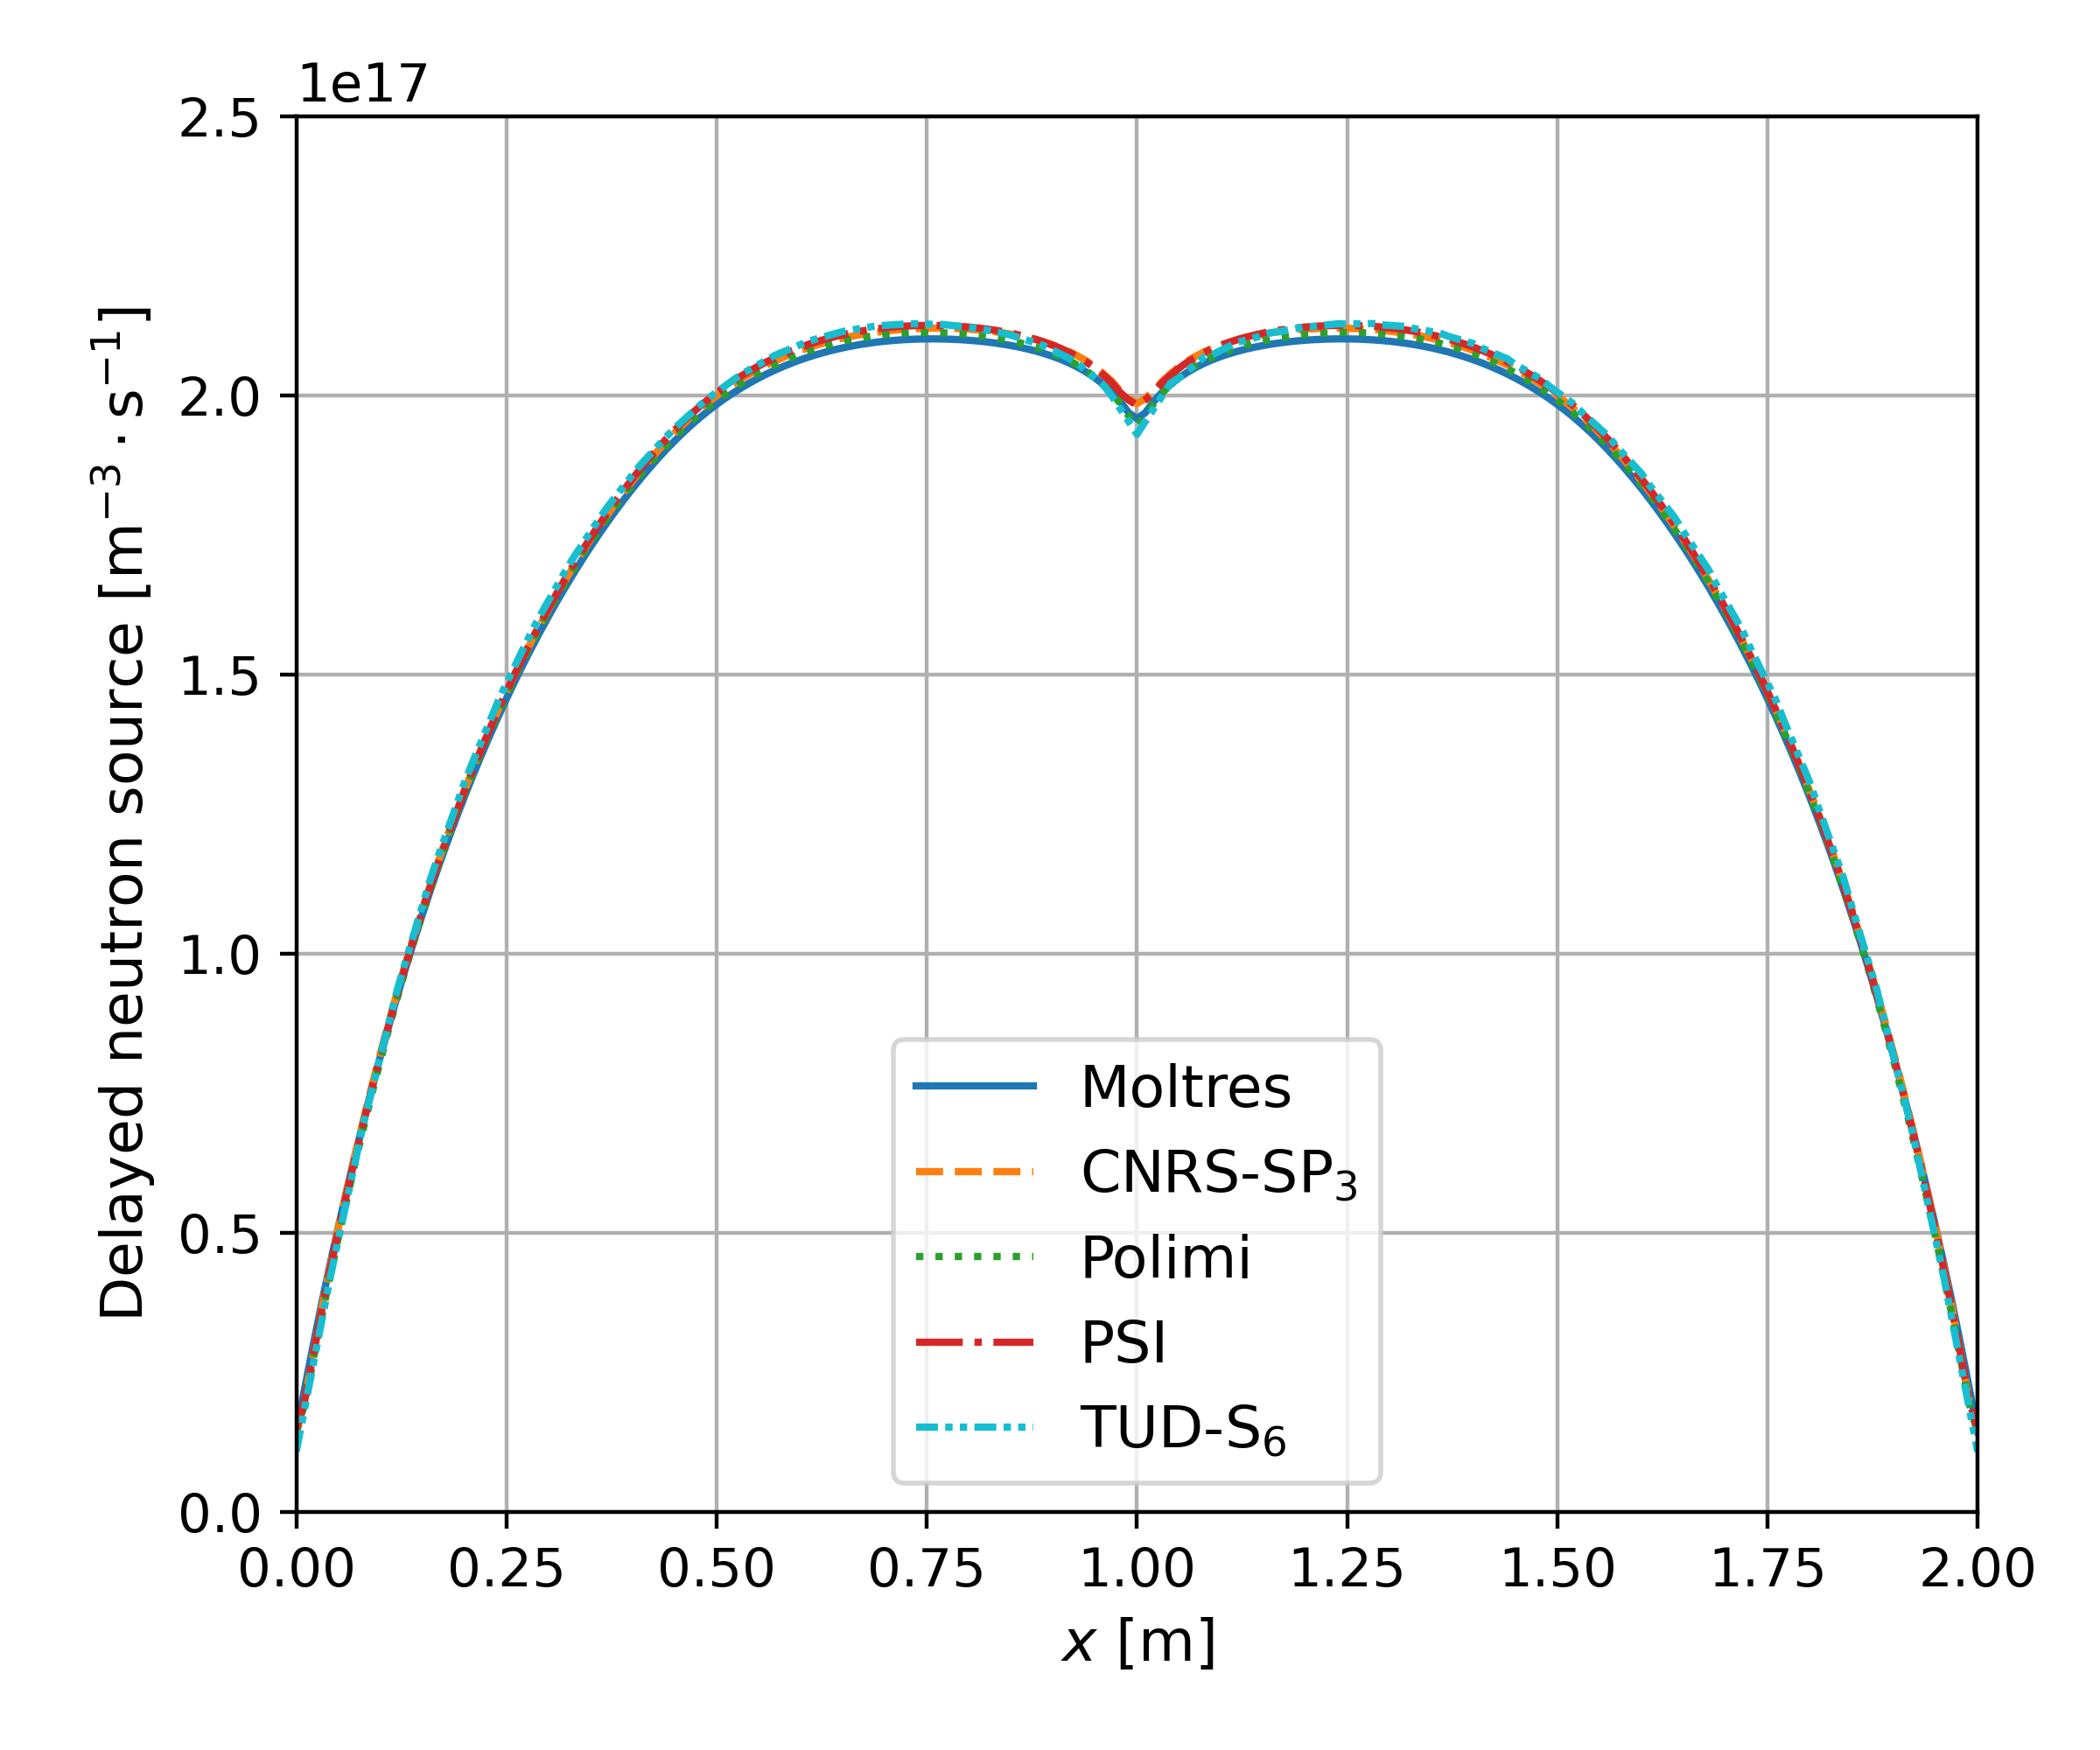
\includegraphics[width=.49\columnwidth]{1-3-dnp-plot}
	\caption{Step 1.3 \textemdash\ Vertical velocity component, temperature distribution,
	and delayed neutron source along AA'.}
	\label{fig:1.3}
\end{figure}

\FloatBarrier

\paragraph{Step 1.4: Full coupling}

Figure \ref{fig:cnrs-color} shows 2D temperature distribution and velocity
streamlines from Moltres for Step 1.4 with $U_{lid} = 0.5$ m$\cdot$s$^{-1}$ and
$P = 1$ GW. Table \ref{table:full} shows the change in $\rho$ under the various
$U_{lid}$ and $P$ values. Refer to Tiberga et al.'s paper
\cite{tiberga_results_2020} for the benchmark participants' corresponding
values. The change in $\rho$ values from Moltres all fall within the range of
benchmark values
for all cases. Furthermore, the $\Delta\rho$ values are all within 1.1 pcm of
the corresponding values from the TUD-S$_2$ model in the benchmark paper. Given
that the $S_2$ discrete ordinates method with isotropic sources is theoretically equivalent to the
multigroup neutron diffusion method, Moltres is largely
consistent with the benchmark participants outside of differences from the
neutronics models.

\begin{figure}[htb]
  \centering
  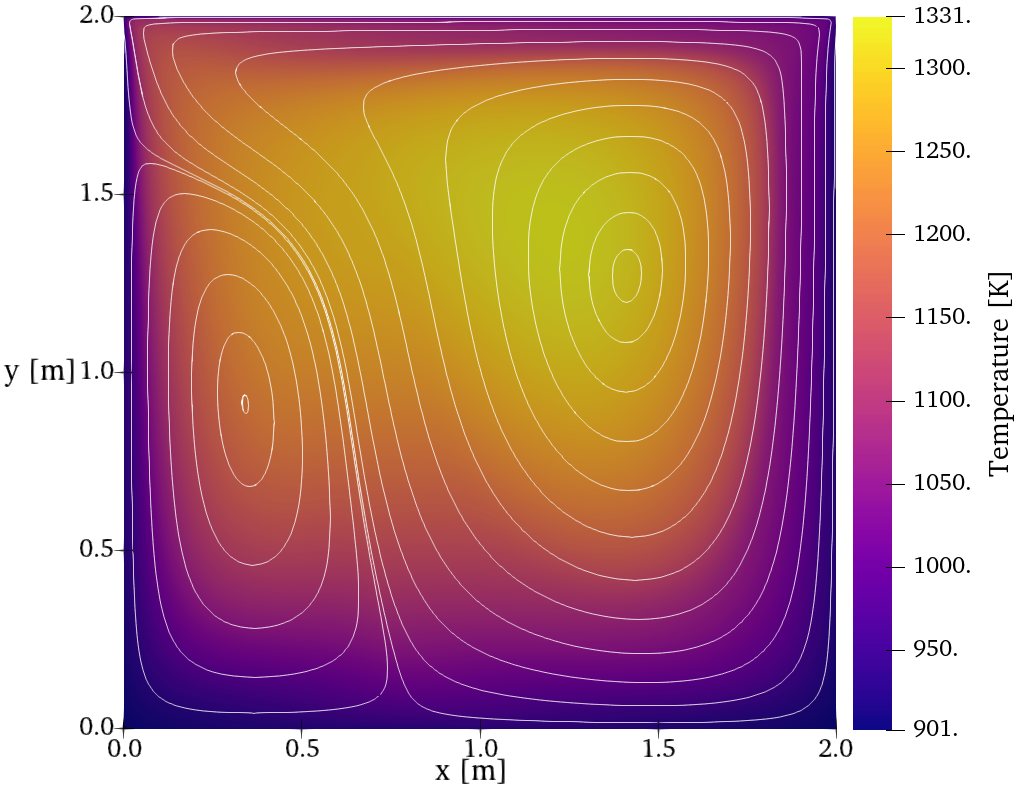
\includegraphics[width=.7\columnwidth]{full-coupled}
  \caption{Temperature distribution from Moltres for the fully coupled
  system (Step 1.4) with buoyancy effects, $P = 1$ GW, and $U_{lid} = 0.5$
  m$\cdot$s$^{-1}$. The lines correspond to the streamlines of the velocity
  field.}
  \label{fig:cnrs-color}
\end{figure}
%
\begin{table}[htb]
	\caption{Reactivity change in Step 1.4, relative to Step 0.2 under various
	$U_{lid}$ and $P$ values.}
	\centering
	\small
	\setlength\tabcolsep{1.5pt}
	\begin{tabular}{c c c c c c}
		\toprule
		& \multicolumn{5}{c}{$\rho_{s1.4} - \rho_{s0.2}$ [pcm]} \\
		\midrule
		{\backslashbox{$U_{lid}$ [m$\cdot$s$^{-1}$]}{$P$ [GW]}} & 0.2 & 0.4 & 0.6 & 0.8 & 1.0 \\
		\midrule
		0.0 & -263.7 & -498.3 & -730.9 & -966.7 & -1207.7 \\
		0.1 & -265.9 & -498.7 & -730.6 & -966.0 & -1206.7 \\
		0.2 & -268.1 & -498.8 & -729.4 & -963.7 & -1203.6 \\
		0.3 & -269.9 & -498.5 & -727.8 & -960.8 & -1199.5 \\
		0.4 & -271.9 & -498.5 & -726.5 & -958.3 & -1195.7 \\
		0.5 & -274.2 & -498.7 & -725.6 & -956.4 & -1192.7 \\
		\bottomrule
	\end{tabular}
	\label{table:full}
\end{table}

\FloatBarrier

\begin{table}[htb]
	\caption{Discrepancy values from Moltres alongside the average and standard
	deviation of the discrepancy values of the benchmark participants for Step
	2.1.}
	\centering
	\small
	\begin{tabular}{l l S S S}
		\toprule
		\multirow{2}{*}{\textbf{Step}} & \multirow{2}{*}{\textbf{Observable}} & {\multirow{2}{*}{\textbf{Moltres [\%]}}} & \multicolumn{2}{c}{\textbf{Benchmark [\%]}} \\
		& & & {Average} & {SD} \\
		\midrule
		\multirow{2}{*}{2.1} & Gain & 0.493 & 0.587 & 0.244 \\
		\cmidrule{2-5}
		& Phase shift & 1.741 & 2.176 & 0.554 \\
		\bottomrule
	\end{tabular}
	\label{table:disc2}
\end{table}
%
\begin{figure}[htb]
	\centering
	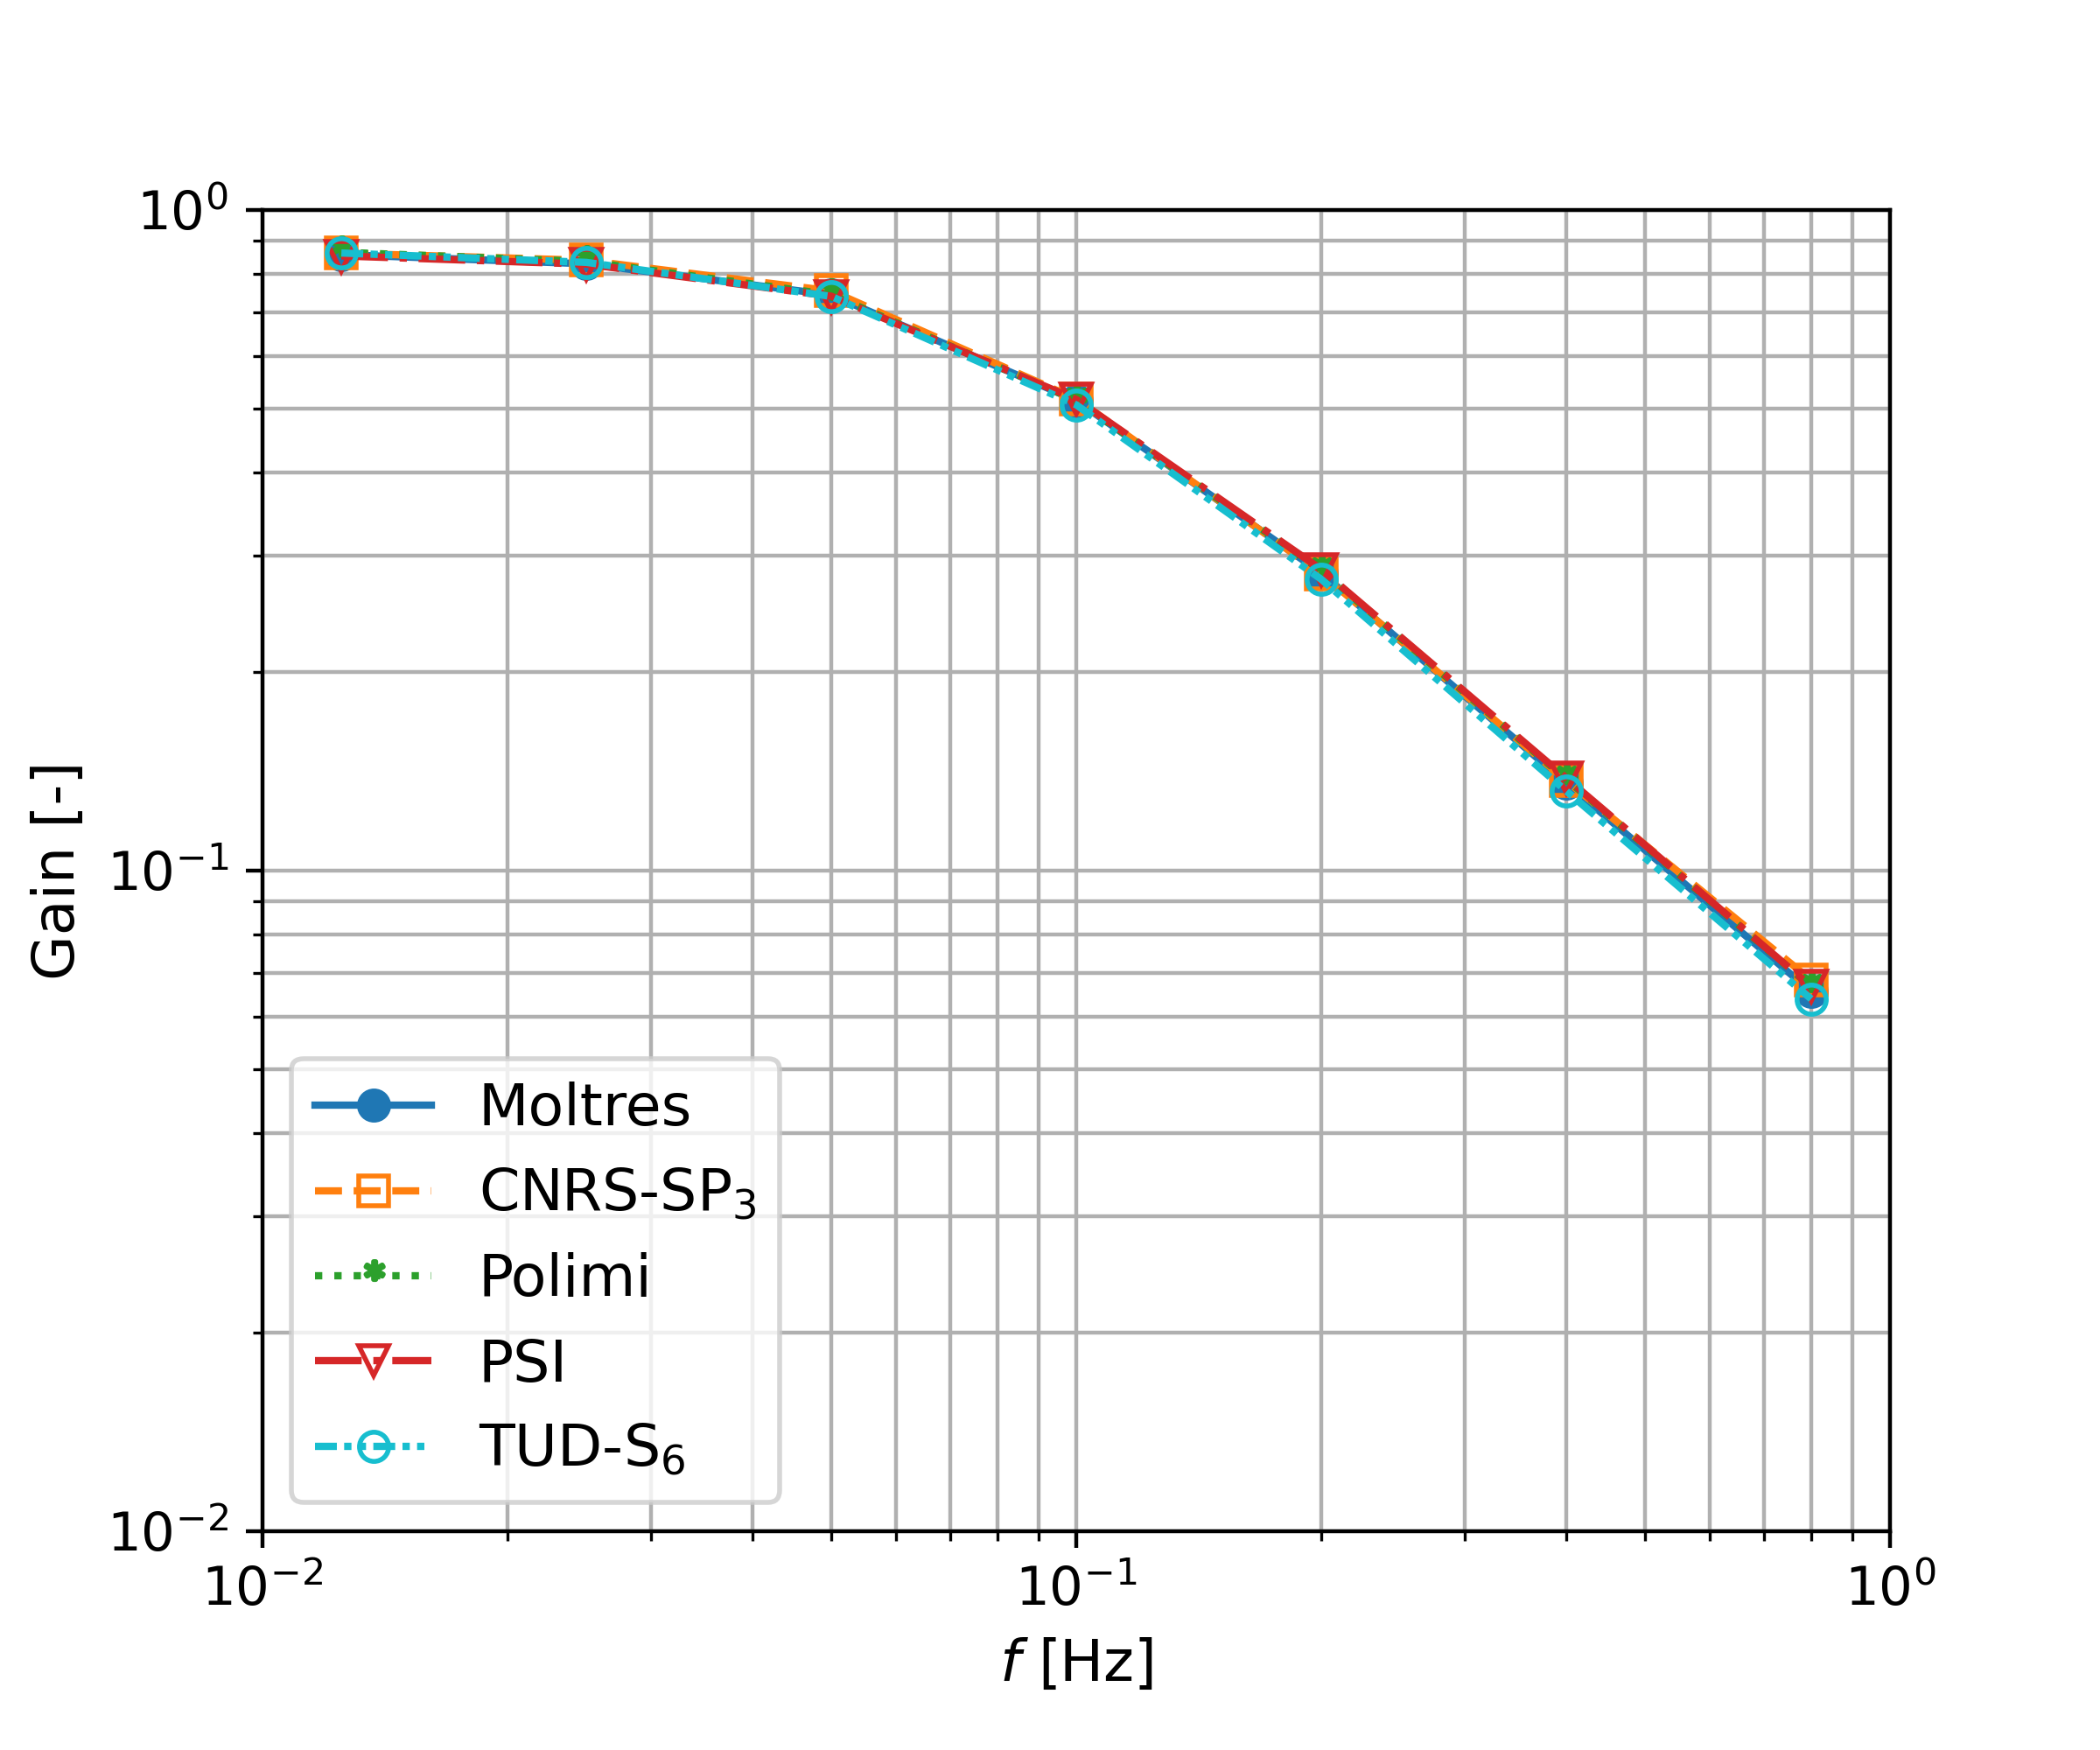
\includegraphics[width=.49\columnwidth]{2-1-gain-plot}
	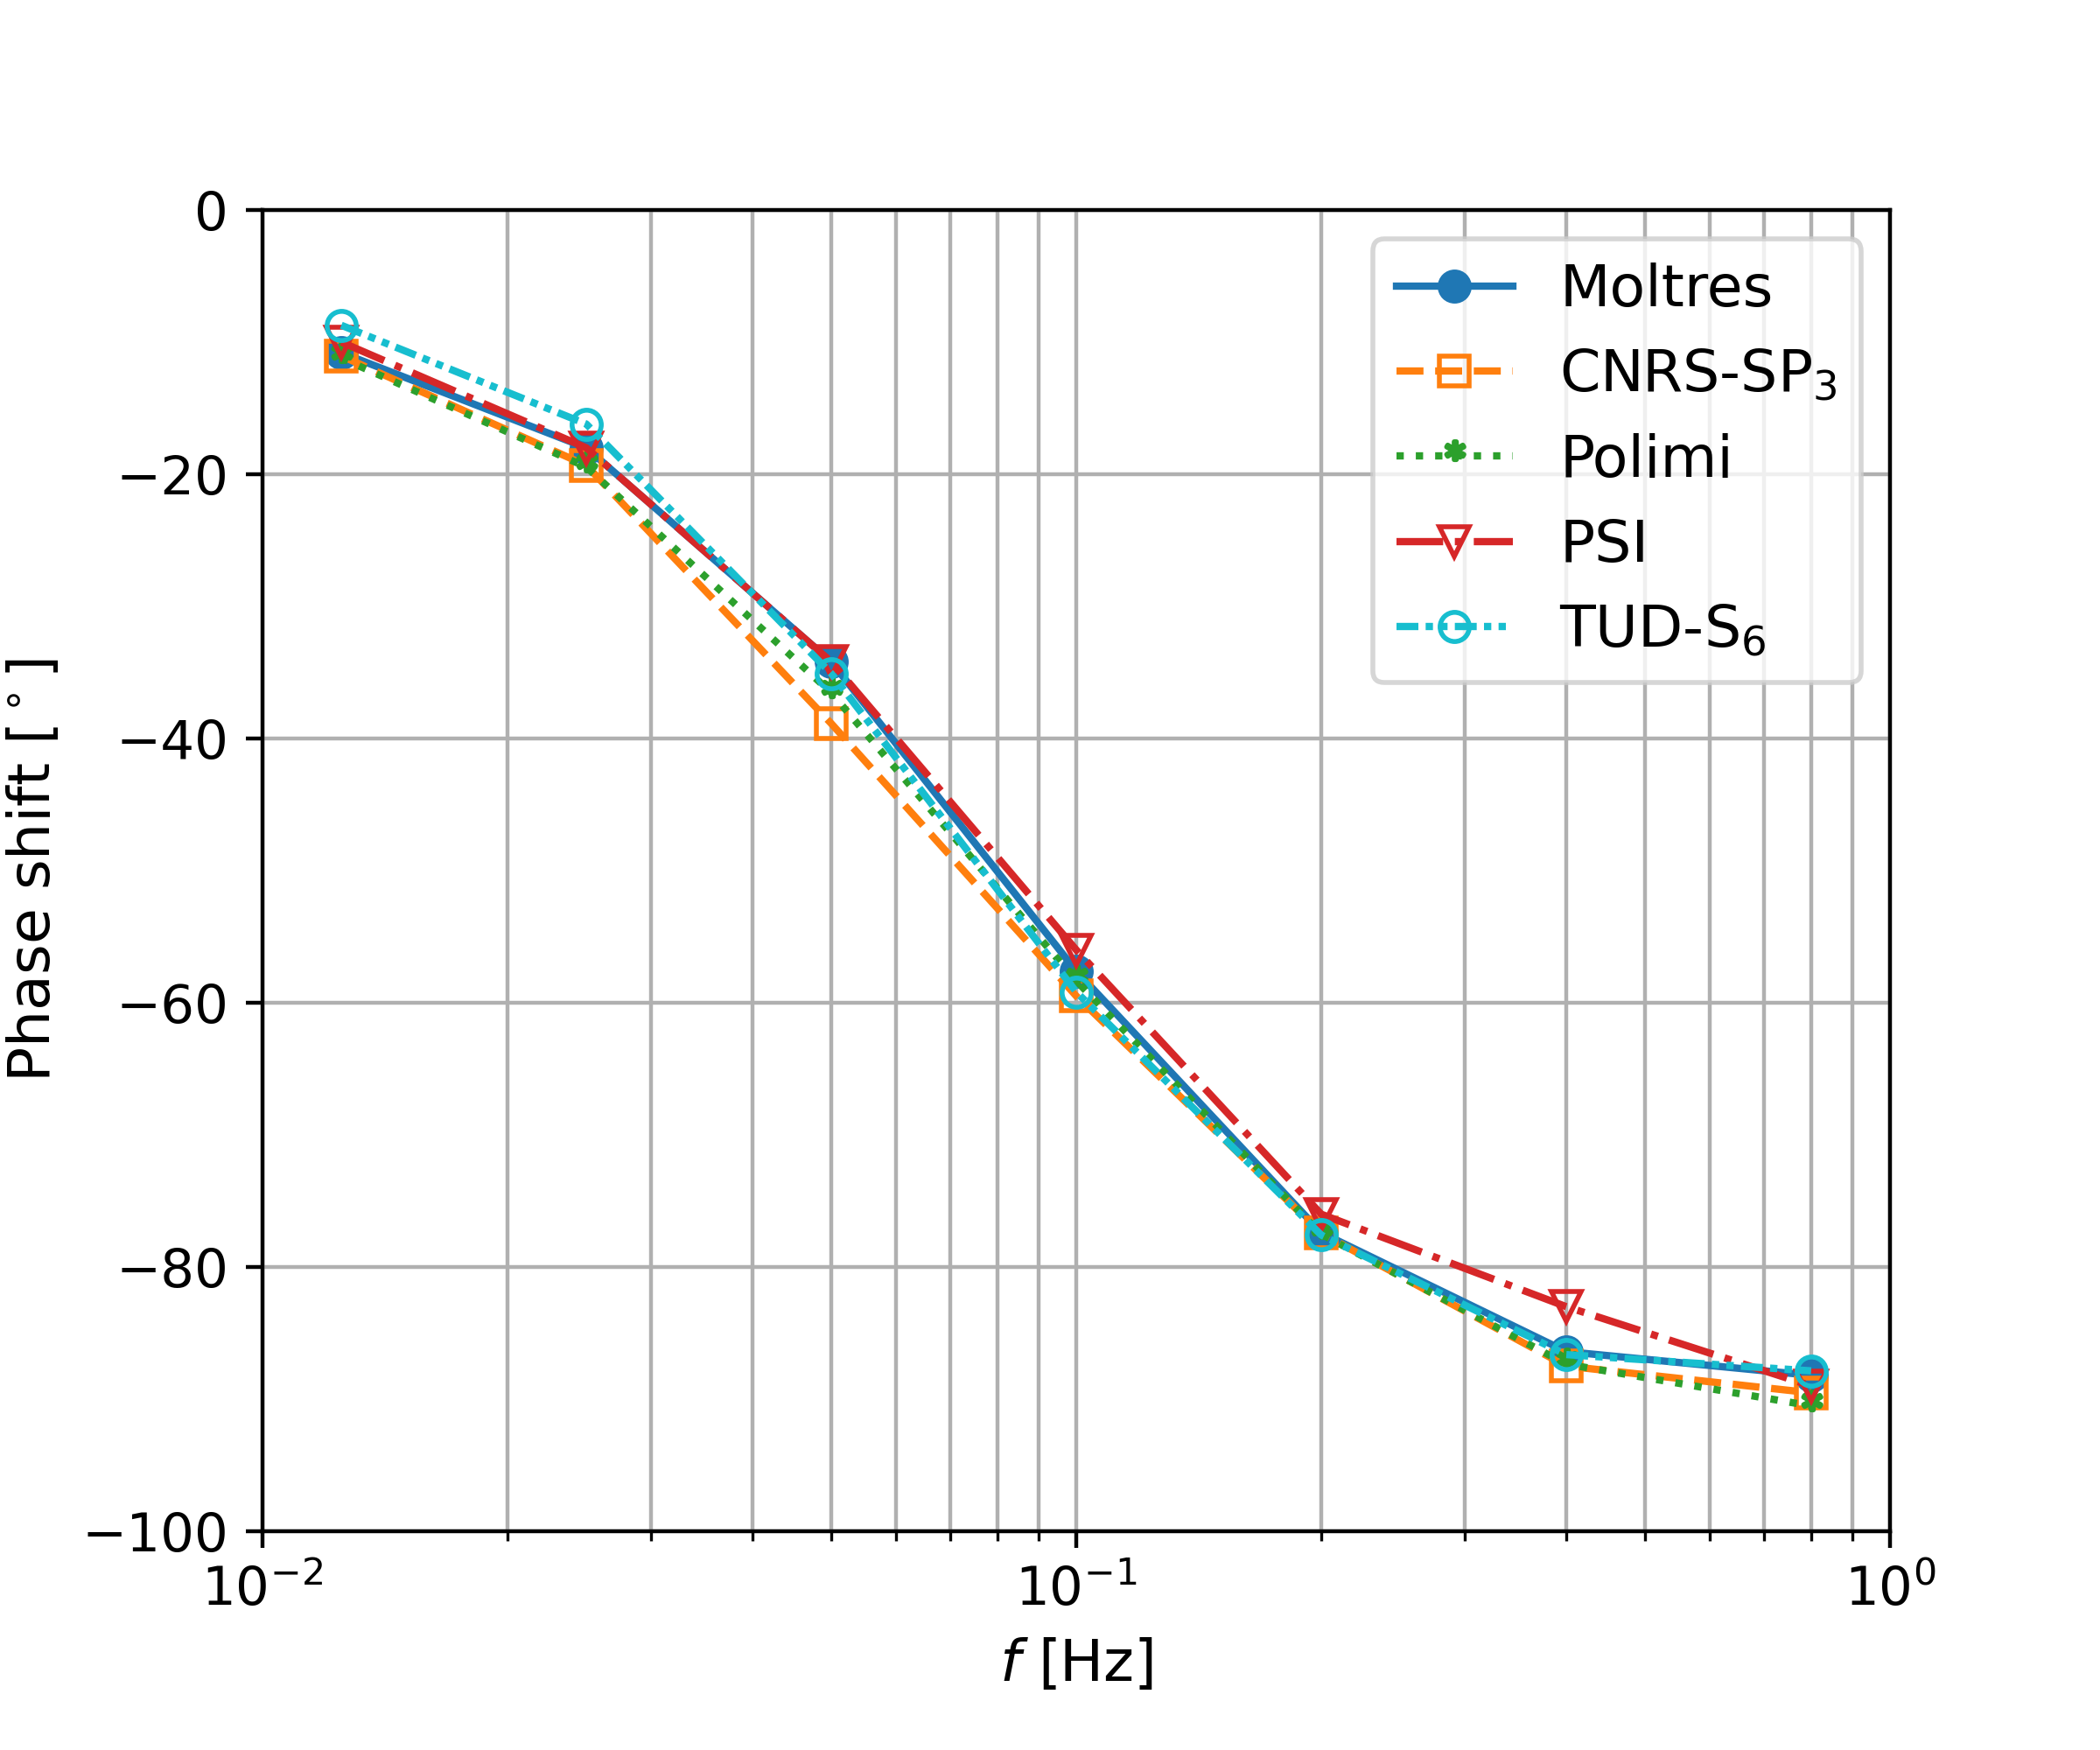
\includegraphics[width=.49\columnwidth]{2-1-phase-plot}
	\caption{Step 2.1 \textemdash\ Bode gain and phase plots of the frequency response of
	the fully coupled system.}
	\label{fig:2.1}
\end{figure}

\subsubsection{Phase 2 results \& discussion}

Lastly, the following subsection discusses the results for the transient cases
in Step 2.1, which involve measuring the response in power output to periodic
perturbations in the heat transfer coefficient.

\paragraph{Step 2.1: Forced convection transient}

Figure \ref{fig:2.1} shows the Bode gain and phase shift plots of the response
in power output in the fully coupled system. Along with the average discrepancy
values from Table \ref{table:disc2}, the results show that Moltres is
consistent with the benchmark. The gain data points from all \gls{MSR} software
agree closely with one another. Moltres reports an average discrepancy value of
0.496\%, slightly lower than the benchmark average of 0.587\%. On the other
hand, the phase shift data points show a greater spread over the various driving
frequencies. We note the different timestepping schemes and timestep
sizes among the different software packages, which is likely responsible for
the variations in the phase shift. Even with a precision of
$\pm0.9^\circ$ for each phase shift value, Moltres accurately reproduces the
correct trend with a lower average discrepancy (1.741\%) than the benchmark
participants' average (2.176\%).

\FloatBarrier

\subsection{Summary}

\glspl{MSR} feature significant multiphysics interactions, presenting
computational challenges for many existing multiphysics reactor analysis
software. This chapter presents code-to-code verification of Moltres'
capabilities in modeling such multiphysics phenomena in fast-spectrum
\glspl{MSR} based on the CNRS benchmark \cite{tiberga_results_2020}.
The CNRS benchmark assesses multiphysics \gls{MSR} simulation
software through several steps involving single-physics and coupled
neutronics/thermal-hydraulics problems.

The results showed that Moltres is consistent with the participating software
presented in the CNRS benchmark paper for modeling important phenomena
in fast-spectrum \glspl{MSR}. The percentage discrepancies in the various
neutronics, velocity, and temperature quantities mostly fall below or within
one standard deviation of the average of the benchmark participants.
Minor deviations in the temperature in Steps 0.3 and 1.2 
stem from the discontinuous velocity
boundaries on the top corners in the lid-driven cavity flow. We have shown that
these deviations are limited to the top boundary of the domain and do not
affect the rest of the physical parameters. The results from
Moltres agree closest with the TUD-S$_2$ software package, which implements the
$S_2$ discrete ordinates method for
neutron transport on a uniform structured mesh with a \gls{DFEM}-based solver.
These features make Moltres the most similar to the TUD-$S_2$ model as compared
to the other models, which employ different neutron transport models,
non-uniform meshes, or finite volume-based solvers.

This work verifies Moltres' capabilities for future work involving the modeling and
simulation of fast-spectrum \glspl{MSR} such as the European \gls{MSFR} and
TerraPower's \gls{MCFR} \cite{terrapower_terrapower_2021}. Notably, the CNRS
benchmark does not assess modeling capabilities for complex physics phenomena
such as turbulent flow in \glspl{MSR}. However, we expect coolant loops in many \gls{MSR} designs
will experience turbulent flow under regular operation or accident scenarios.
These expectations, alongside the subpar results of pump-initiated accidents
reported in Section \ref{sec:msfr}, call for the implementation and
verification of a turbulence model in Moltres to accurately model \glspl{MSR}.

\FloatBarrier



This section covers a \gls{VV} study based on the \gls{MSRE} zero-power pump
start-up and coast-down pump transient tests. In collaboration with Aaron Reynolds (formerly from
Oregon State University, we verified and validated the looped \gls{DNP} flow modeling capability of
our respective reactor simulation software, Moltres and QuasiMolto \cite{reynolds_analysis_2023}.

\subsection{Description of MSRE Pump Transient Tests}

The \gls{MSRE} was an experimental molten salt reactor constructed and operated at \gls{ORNL} in
the 1960s \cite{haubenreich_experience_1970}. It is a 8-MW$_{\text{th}}$, thermal-spectrum reactor
with a graphite moderator and a LiF-BeF$_2$-ZrF$_4$-UF$_4$ fuel-molten salt mixture. Under normal
power operation, the fuel salt flows out of the core and deposits heat in the heat exchanger before
being pumped back into the core. Due to
\glspl{DNP} being produced in the molten salt coolant, flow rates have significant impacts on the
\gls{DNP} distribution and reactivity. Delayed neutrons born in regions of lower neutronic
importance, e.g., at the periphery or outside the core, are more likely to be lost through neutron
leakage or parasitic absorption.

\begin{figure}[htb]
  \centering
  \begin{minipage}[t]{0.49\textwidth}
    \centering
    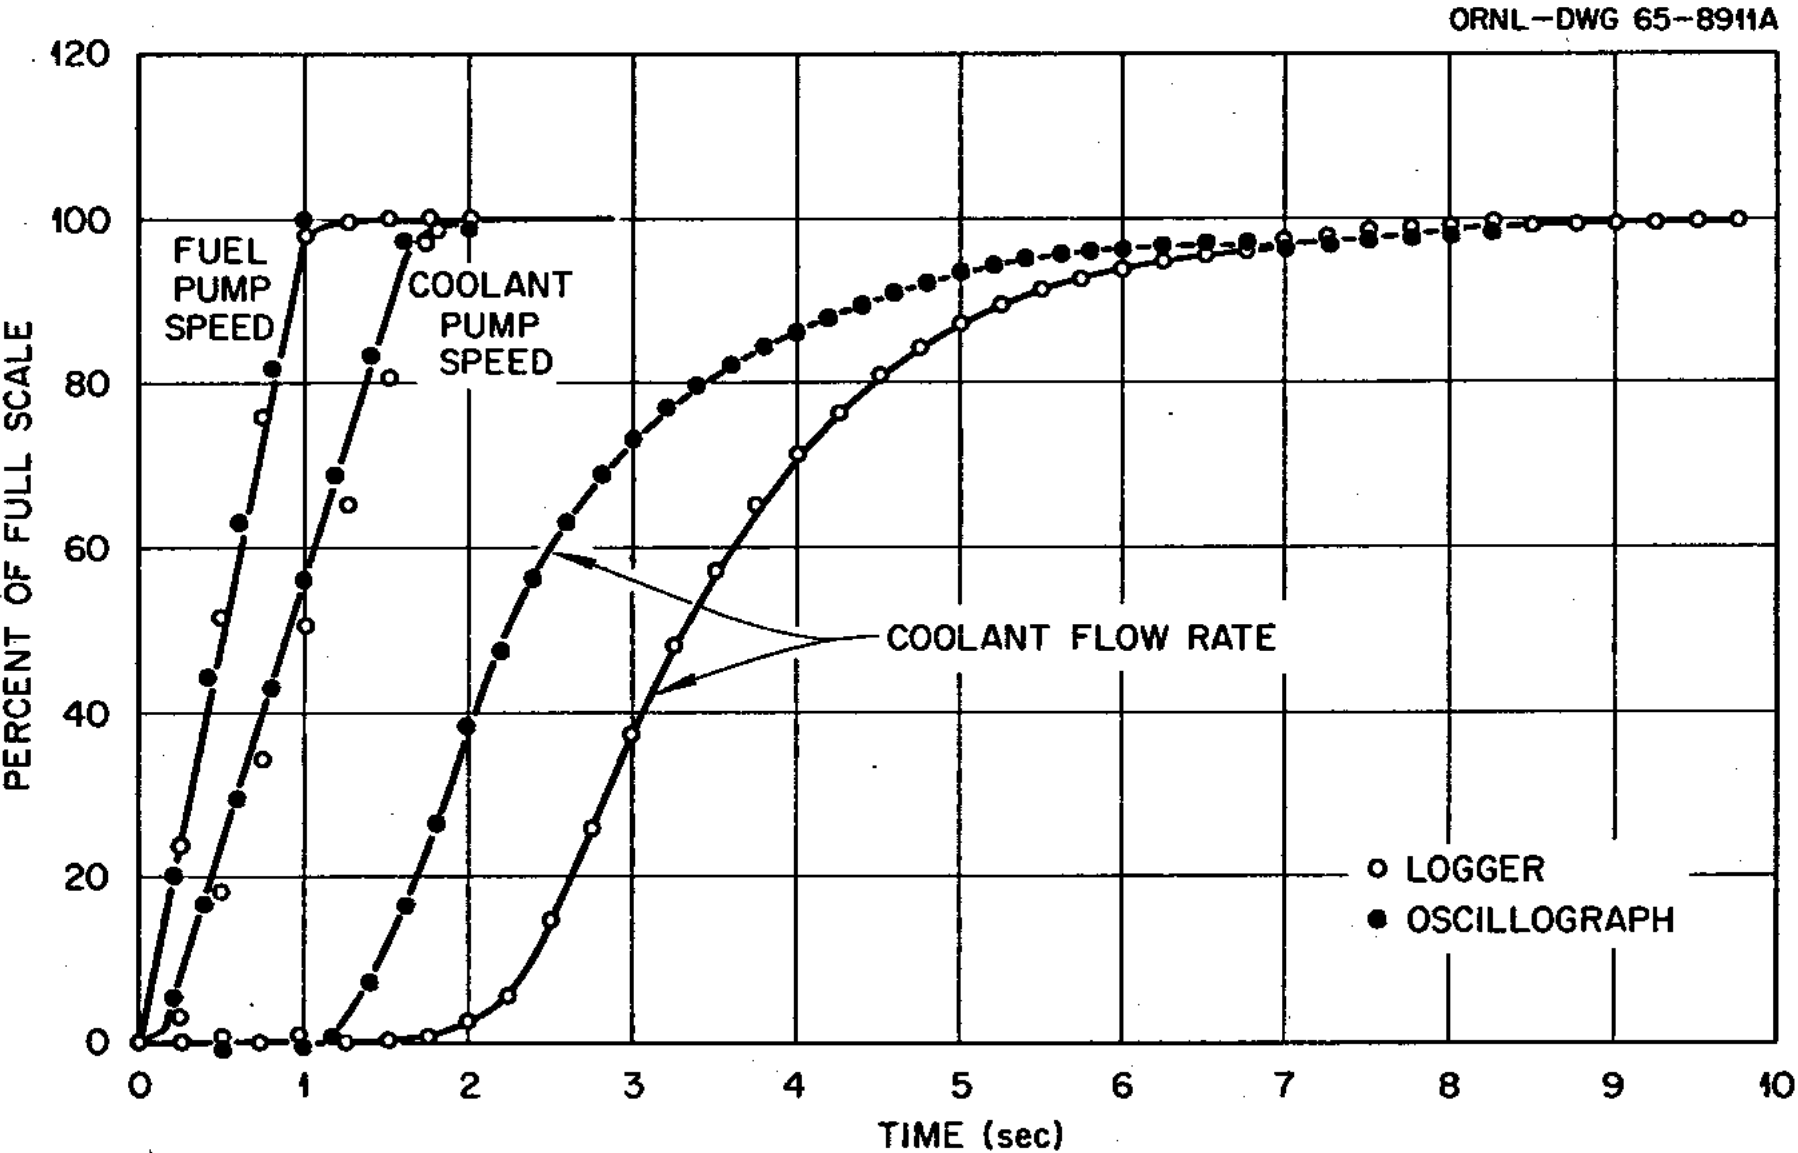
\includegraphics[width=\columnwidth]{msre-startup}
    \caption{Start-up pump speed and coolant flow rate \cite{prince_zero-power_1968}.}
    \label{fig:msre-startup}
  \end{minipage}
  \hfill
  \begin{minipage}[t]{0.49\textwidth}
    \centering
    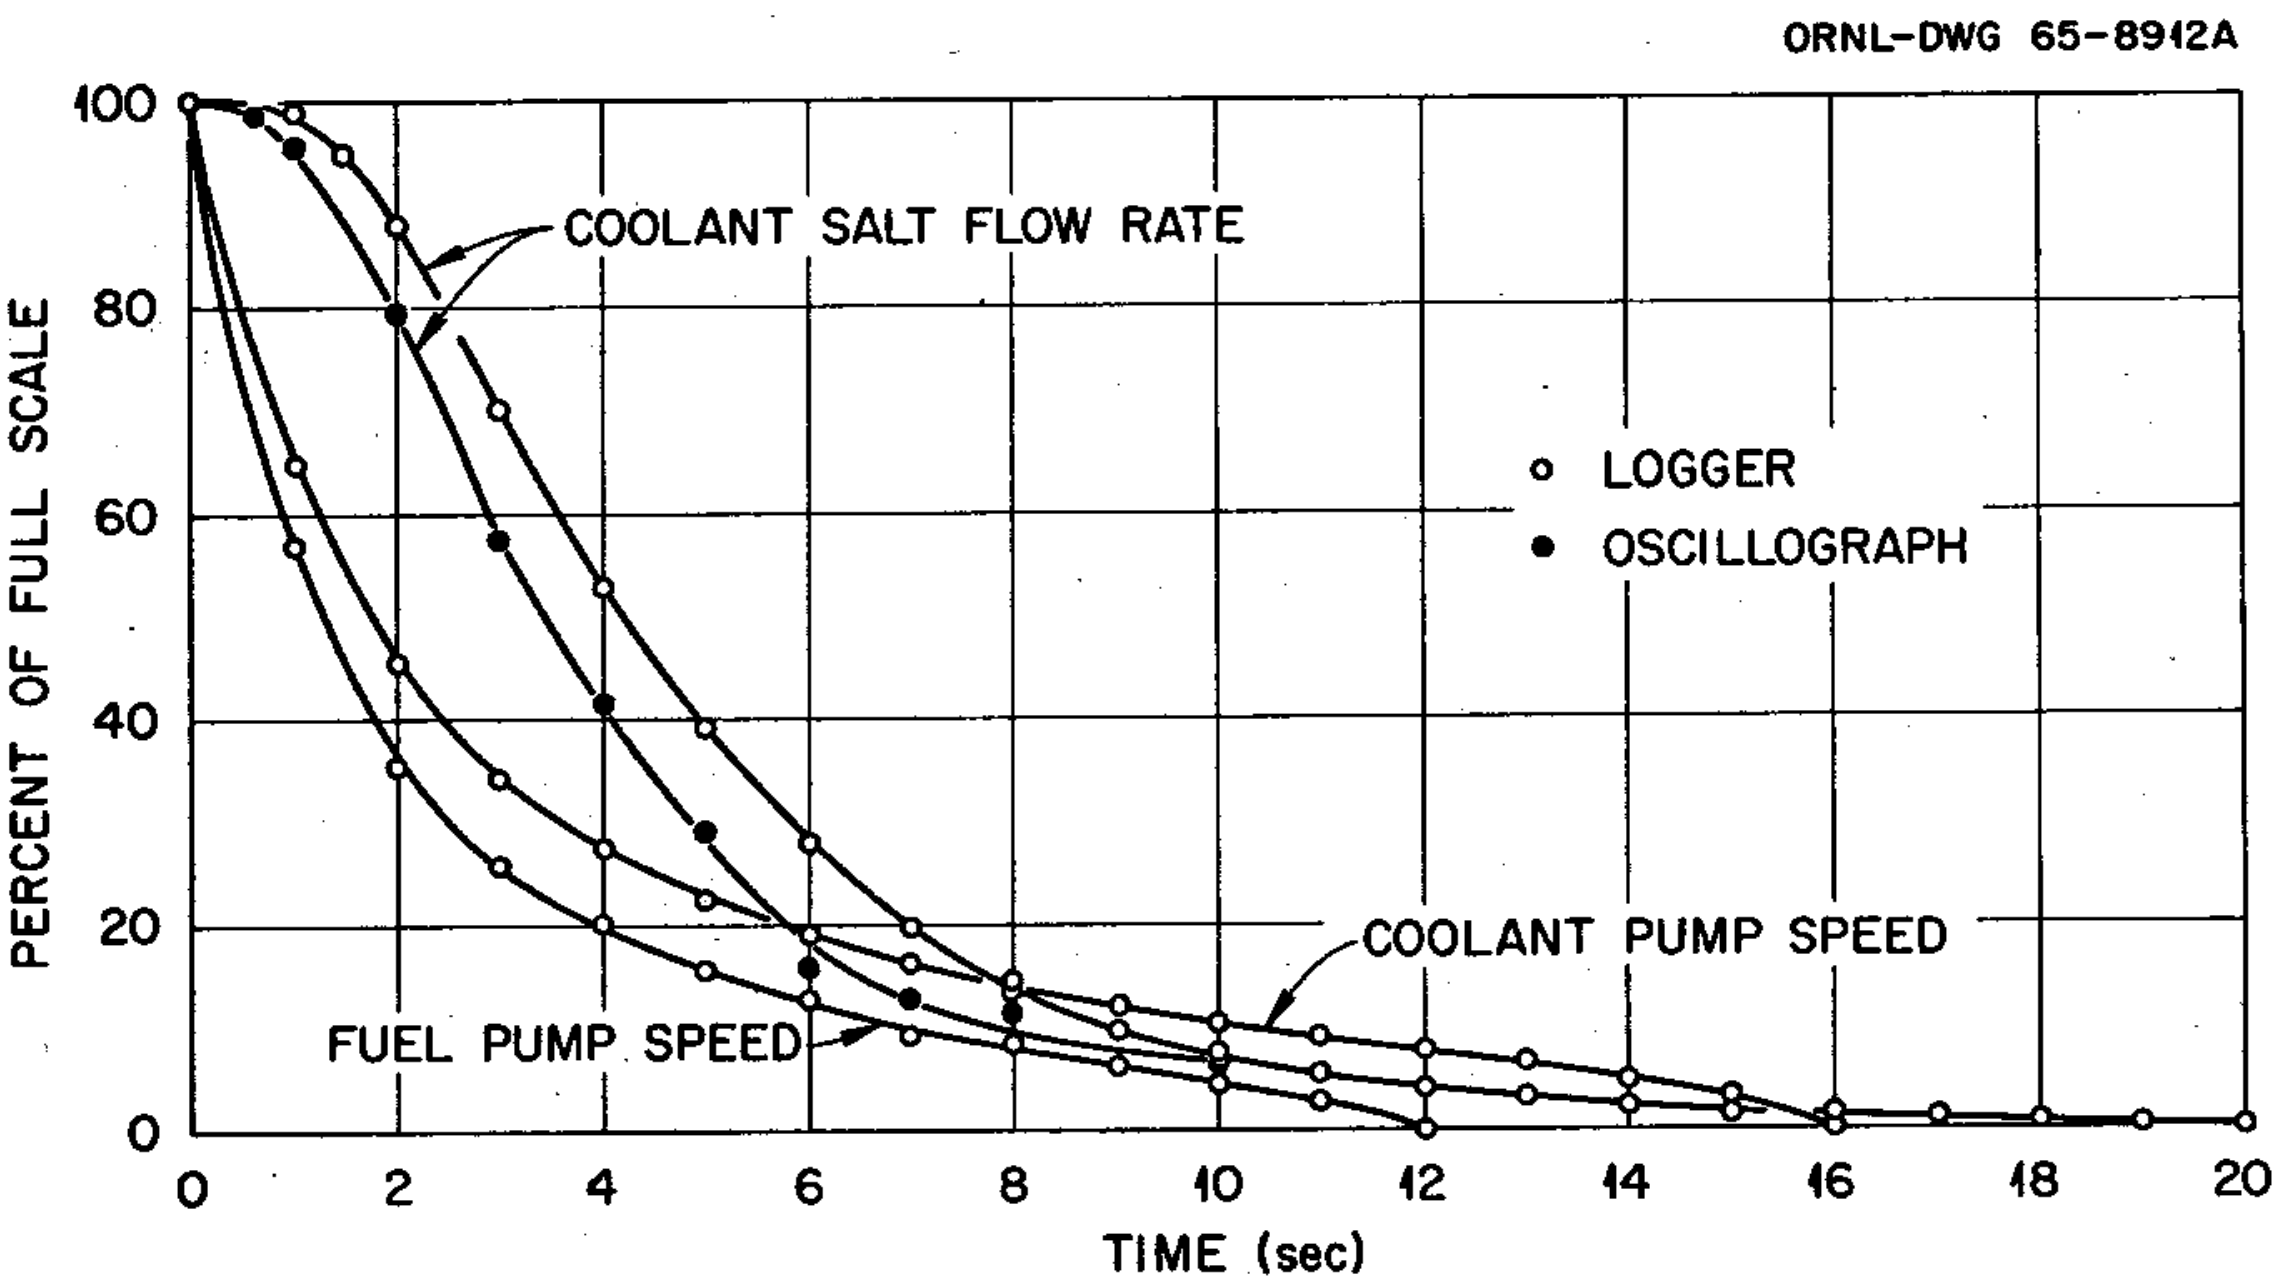
\includegraphics[width=\columnwidth]{msre-coastdown}
    \caption{Coast-down pump speed and coolant flow rate \cite{prince_zero-power_1968}.}
    \label{fig:msre-coastdown}
  \end{minipage}
\end{figure}

\gls{ORNL} researchers performed fuel pump start-up and coast-down transient experiments to
determine the ``transient effects of fuel flow-rate changes on reactivity''
\cite{prince_zero-power_1968}. These experiments were a part of \gls{MSRE} zero-power dynamics
tests performed in June 1965, the same month the \gls{MSRE} achieved initial criticality. Figures
\ref{fig:msre-startup} and \ref{fig:msre-coastdown} show the pump speeds and secondary salt coolant
flow rates measured during the transients. The changing flow rates caused advective changes to the
\gls{DNP} distribution and the \gls{DNF} in the reactor core.

During both experiments, the reactivity effects of the \gls{DNP} drift were measured by
allowing the flux servo controller to maintain criticality. The controller maintained core
criticality by adjusting the control rod insertion height in response to \gls{DNP} drift-induced
reactivity changes. The reactivity changes over time can be calculated by comparing the various
control rod positions (Figure \ref{fig:msre-pump-rod}) with the control rod integral worth curve
(Figure \ref{fig:msre-rod-worth}) obtained during control rod calibration experiments.

\begin{figure}[htb]
  \centering
  \begin{minipage}[t]{0.49\textwidth}
    \centering
    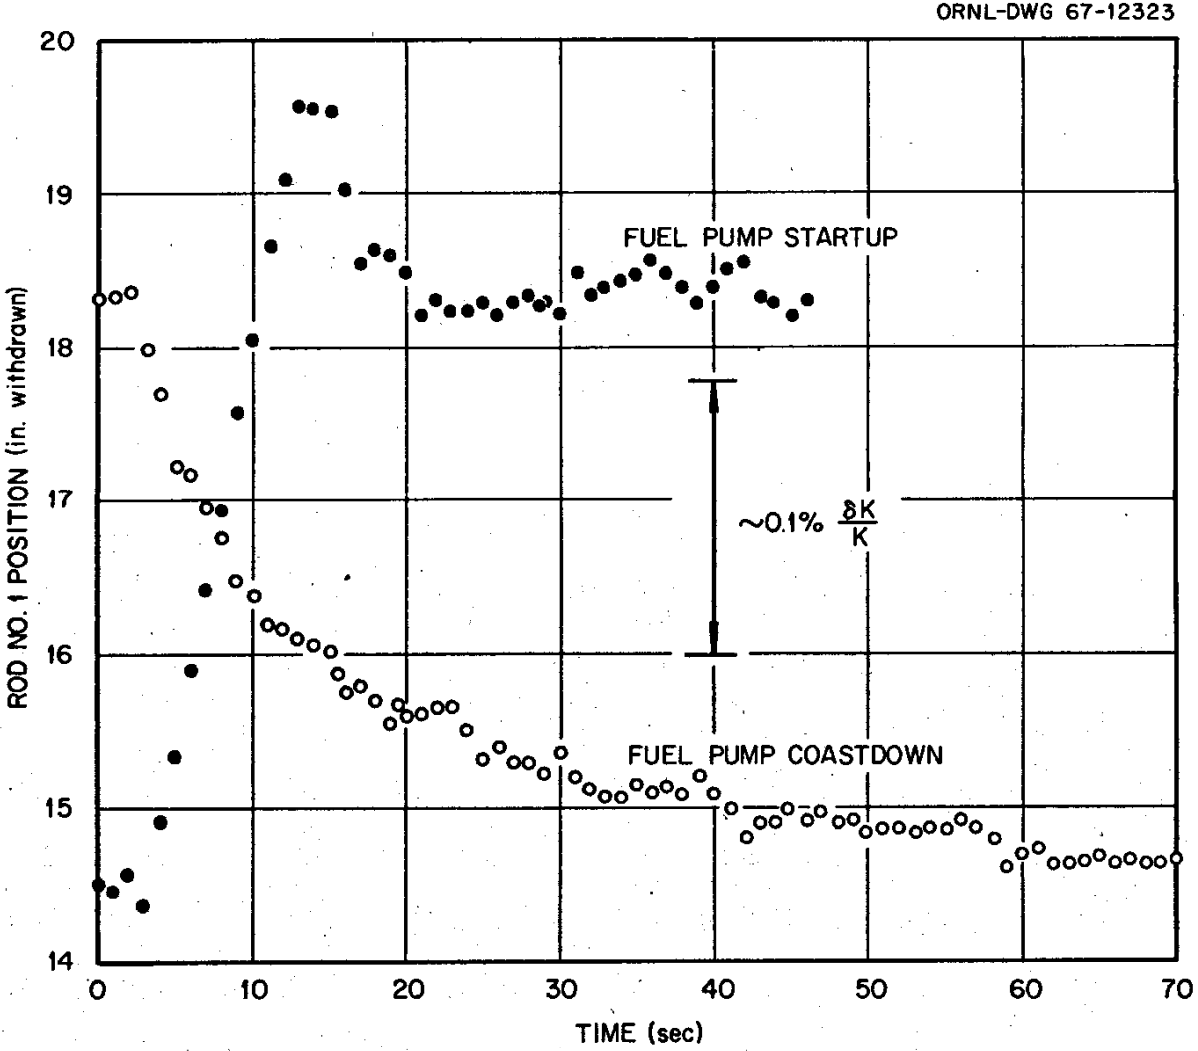
\includegraphics[width=\columnwidth]{msre-transient}
    \caption{Control rod response to fuel pump start-up and coast-down
    \cite{prince_zero-power_1968}.}
    \label{fig:msre-pump-rod}
  \end{minipage}
  \hfill
  \begin{minipage}[t]{0.49\textwidth}
    \centering
    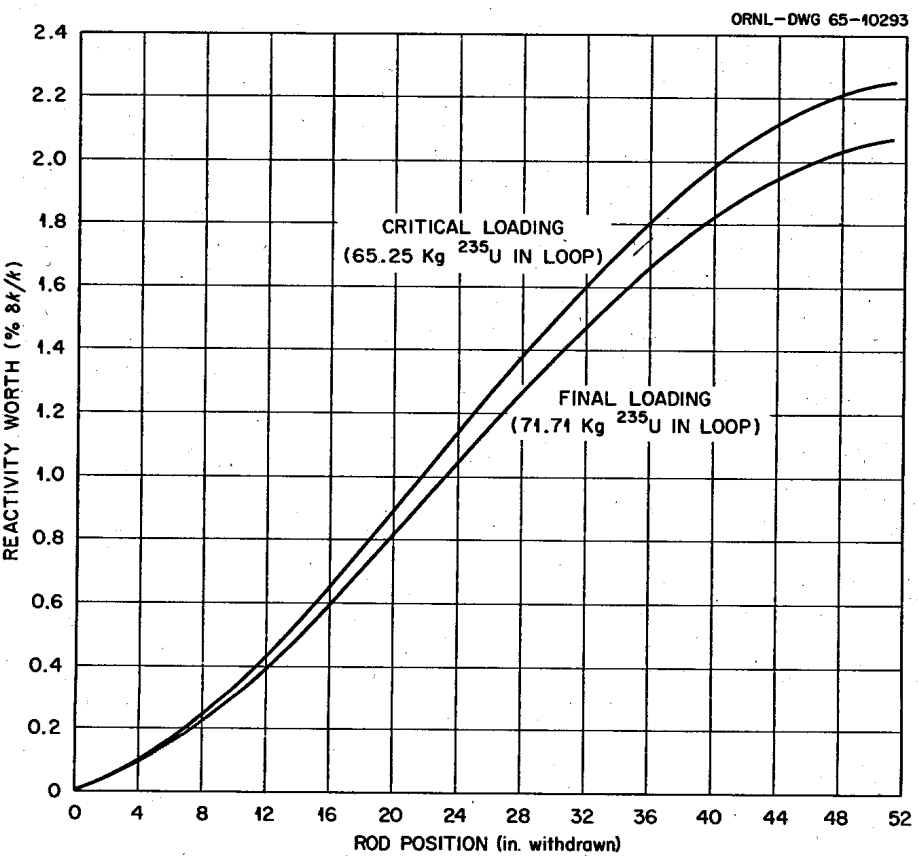
\includegraphics[width=\columnwidth]{msre-rod-worth}
    \caption{Integral control rod worth of Rod 1 \cite{prince_zero-power_1968}.}
    \label{fig:msre-rod-worth}
  \end{minipage}
\end{figure}

\subsection{Description of QuasiMolto}

QuasiMolto \cite{reynolds_analysis_2023} is an open-source multiphysics research code for
simulating circulating fuel reactor kinetics. It uses the multilevel \gls{QD} methodology described
in Section \ref{sec:lit-tc} to model multigroup neutron transport with \gls{DNP} flow and
temperature advection-diffusion. Consisting of three levels of neutron calculations, the highest
level solves the multigroup high-order transport equations for Eddington and boundary factors which
populate previously unknown quantities in the mid-level multigroup low-order \gls{QD} equations.
In turn, the mid-level equations solve for group-collapsed Eddington and boundary factors for the
low-level effective low-order transport equations. The effective low-order transport equations
couple with the \gls{DNP} and temperature governing equations for multiphysics reactivity feedback
from temperature and \gls{DNP} flow. Readers may refer to the linked reference
\cite{reynolds_analysis_2023} for more details on QuasiMolto.

QuasiMolto applies the simple corner balance method
\cite{adams_subcell_1997} for spatial discretization.
For this study, the QuasiMolto \gls{MSRE} model employed $S_2$ neutron transport to facilitate
fair comparisons with the neutron diffusion method in Moltres. For time-dependent \gls{DNP} flow
modeling, QuasiMolto applies implicit Euler scheme for the reaction
and diffusion terms, and explicit Superbee flux limiter scheme for the advection term.

\subsection{Modeling Approach}

For this study, we adopted a 2-D axisymmetric (R-Z) model of the \gls{MSRE} consisting of
alternating vertical regions of molten salt and graphite moderator. This is the same \gls{MSRE}
model Reynolds developed for his PhD thesis \cite{reynolds_multilevel_2020} and a related
journal publication \cite{reynolds_analysis_2023}. Figure \ref{fig:pump-geom} depicts the 2-D
axisymmetric \gls{MSRE} model. The fuel salt channels are 1.25-cm wide and spaced at 5-cm intervals
in the graphite matrix. The fuel salt volume fraction of this model is 0.236, differing
slightly to the \gls{MSRE} design specification of 0.225 \cite{robertson_msre_1965}. The geometry
mesh is uniform with a width of $\Delta r=0.078125$ cm and height of $\Delta z=5$ cm.
Vacuum boundary conditions for the neutron flux apply along the top, bottom, and right boundaries.

The salt flows
upwards at a spatially uniform velocity rate of 18.085 cm s$^{-1}$. \glspl{DNP} flow out of the
core model and through a separate 285-cm long 1-D pipe model before being reintroduced through the
bottom core channel inlets. The 1-D pipe length maintains the overall salt circulation time of
25.2 s from the \gls{MSRE} design specification \cite{robertson_msre_1965}. Note that the salt
velocity and 1-D pipe length in this study differs from the \gls{MSRE} model described in Reynolds'
paper \cite{reynolds_analysis_2023}. We reduced the velocity to compensate for the absence of upper
and lower core plena by extending salt residence time in the salt-graphite lattice region.

\begin{figure}[htb]
  \centering
  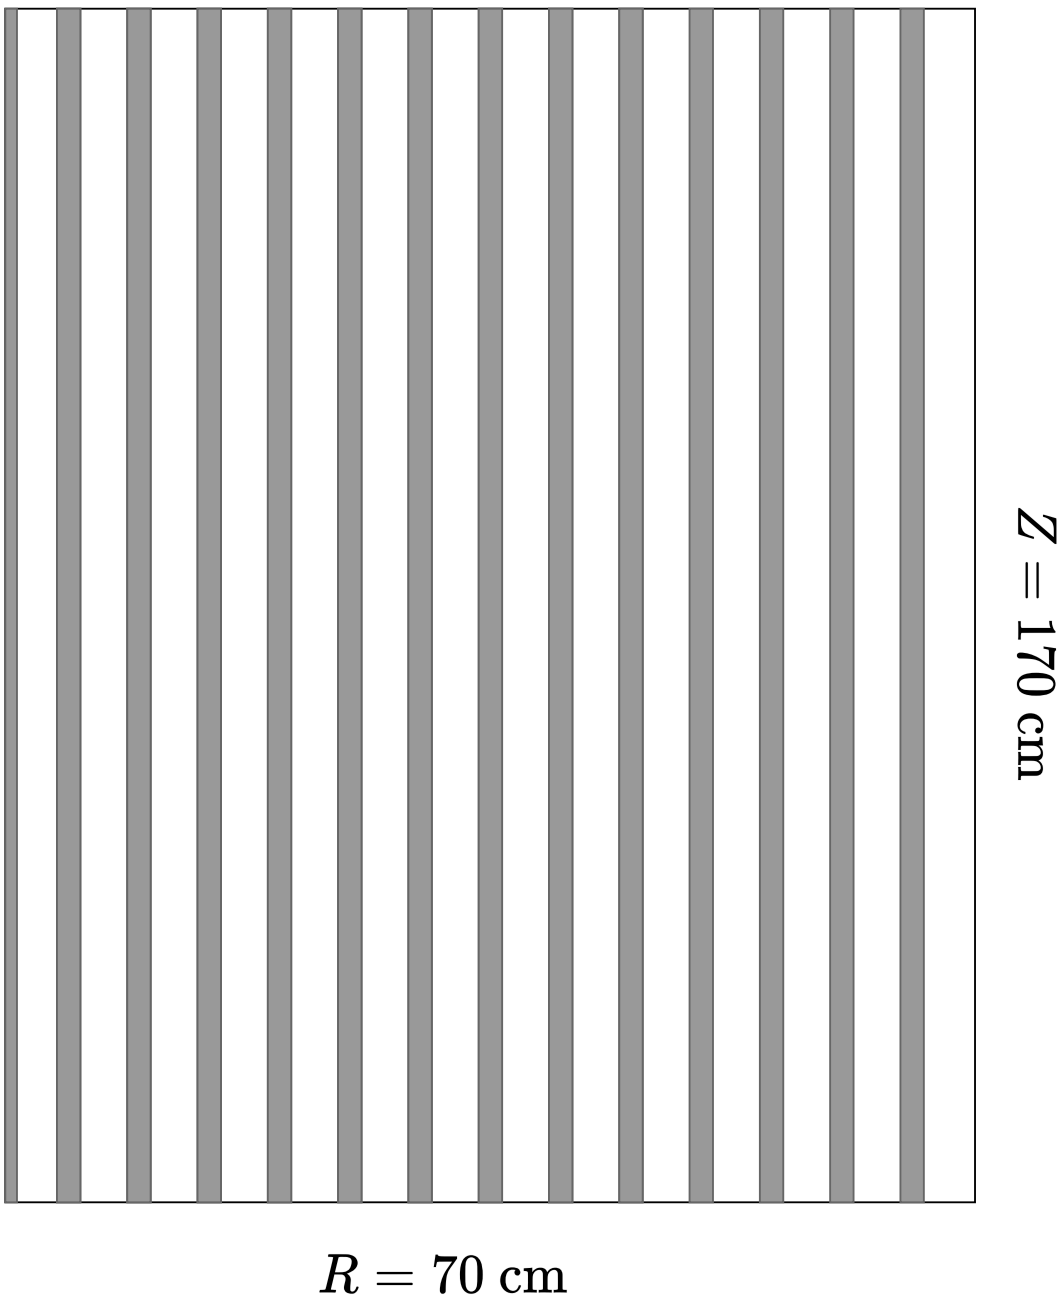
\includegraphics[width=0.6\columnwidth]{msre-2d}
  \caption{2-D axisymmetric model of the \gls{MSRE}.The gray and white regions represent fuel salt
  and graphite, respectively. The leftmost fuel salt channel falls along the axis of symmetry and
  is half-width. Not drawn to scale.}
  \label{fig:pump-geom}
\end{figure}

Reynolds generated group constants for two neutron energy groups and six \gls{DNP} groups using the
NEWT transport module within the SCALE code system \cite{rearden_scale_2018} and the ENDF/B-VII
nuclear data library \cite{chadwick_endf/b-vii.1_2011}. The SCALE model geometry comprised a
representative unit cell geometry
consisting of a circular fuel region in the center of a square graphite region and reflective
boundary conditions on all boundaries. The unit cell dimensions preserved material compositions
and salt-to-graphite ratios from the \gls{MSRE} design specifications.

Prior to the pump transient simulations, we performed code-to-code verification by comparing the
$k_\text{eff}$ and neutron flux and \gls{DNP} distributions of the 2-D \gls{MSRE} model under
static, no salt flow conditions. We sampled the neutron flux and \gls{DNP} distributions on
mesh corners and edge centers along the centerline ($r=0$ cm) and midplane ($z=85$ cm) of the
reactor geometry.

In lieu of reactivity control using a control rod in the pump
transient simulations, QuasiMolto and Moltres solved their respective
two-group $k$-eigenvalue neutronics models at every time-step. The $1/k_\text{eff}$ scaling factor
in the fission neutron source term keeps the simulation at a pseudo-critical state. The \gls{DNP}
source term is also scaled by $1/k_\text{eff}$ at every time-step. We interpolated the \gls{MSRE}
salt flow velocity data in Figures \ref{fig:msre-startup} and \ref{fig:msre-coastdown} to apply in
our pump start-up and coast-down simulations. The pump start-up simulation starts from a static
state with no salt flow while the pump coast-down simulation starts from a steady flow state with
operating salt flow.

\subsection{Results \& Discussion}

We start with a comparison of the Moltres and QuasiMolto \gls{MSRE} numerical models under static
and steady salt flow conditions. Table \ref{table:msre-pump-keff} lists the $k_\text{eff}$
estimates under static and steady flow conditions, and the reactivity changes due to \gls{DNP}
flow. Moltres and QuasiMolto show excellent agreement with 22 and 21 pcm absolute differences in
$k_\text{eff}$ under static and steady flow conditions, respectively. Consequently, the
$\Delta\rho$ estimates from \gls{DNP} flow fall within 1 pcm difference of each other.

\begin{table}[htb]
  \centering
  \caption{Multiplication factors $k_\text{eff}$ under static and steady salt flow conditions, and
  reactivity changes $\Delta\rho$ due to \gls{DNP} flow from the Moltres and QuasiMolto \gls{MSRE}
  models.}
  \begin{tabular}{l S S S}
    \toprule
    \multirow{2}{*}{Code} & \multicolumn{2}{c}{$k_\text{eff}$} & {$\Delta\rho$ due to} \\
                          & {Static} & {Steady flow} & {\gls{DNP} flow} \\
                          \cmidrule(r){1-1} \cmidrule(rl){2-3} \cmidrule(l){4-4}
    Moltres & 1.05625 & 1.05311 & -282.4 \\
    QuasiMolto & 1.05603 & 1.05290 & -281.7 \\
    \bottomrule
  \end{tabular}
  \label{table:msre-pump-keff}
\end{table}

Moving on to comparing spatial distributions, we start with the centerline neutron flux
distributions. Figure \ref{fig:centerline-flux-dist} shows the normalized group 1 and 2 neutron
fluxes exhibiting nearly perfect overlap. The flux ratio distributions in Figure
\ref{fig:centerline-flux-ratio} illustrate the strong agreement between Moltres and QuasiMolto at
all sampled locations with the relative differences falling below 0.8\%. We attribute
the oscillations in the flux ratios to differences in spatial discretization schemes. Moltres
uses \gls{FEM} with 1st-order flux values computed at the mesh corners. QuasiMolto uses
the simple corner balance method which subdivides each mesh element into four equal subcells and
computes volume-averaged flux values in each subcell. As such, Moltres and QuasiMolto require
interpolation for sampling mesh edge center and mesh corner values, respectively. The flux ratios
sampled at the top and bottom boundaries show the greatest differences of up to 0.8\%. We attribute
these differences at the boundaries to differences in neutronics methods. The neutron diffusion
method vacuum boundary condition in Moltres depends on the scalar flux gradient (1-st
order derivative) while the $S_2$ method vacuum boundary condition in QuasiMolto depends on the
angular flux value. Combined with the different spatial discretization schemes, flux differences at
the boundary are expected in numerical calculations. Nevertheless, the overall ratio magnitudes
remain small, thereby supporting code-to-code consistency between Moltres and QuasiMolto.

\begin{figure}[htb]
  \centering
  \begin{subfigure}[b]{0.48\columnwidth}
    \centering
    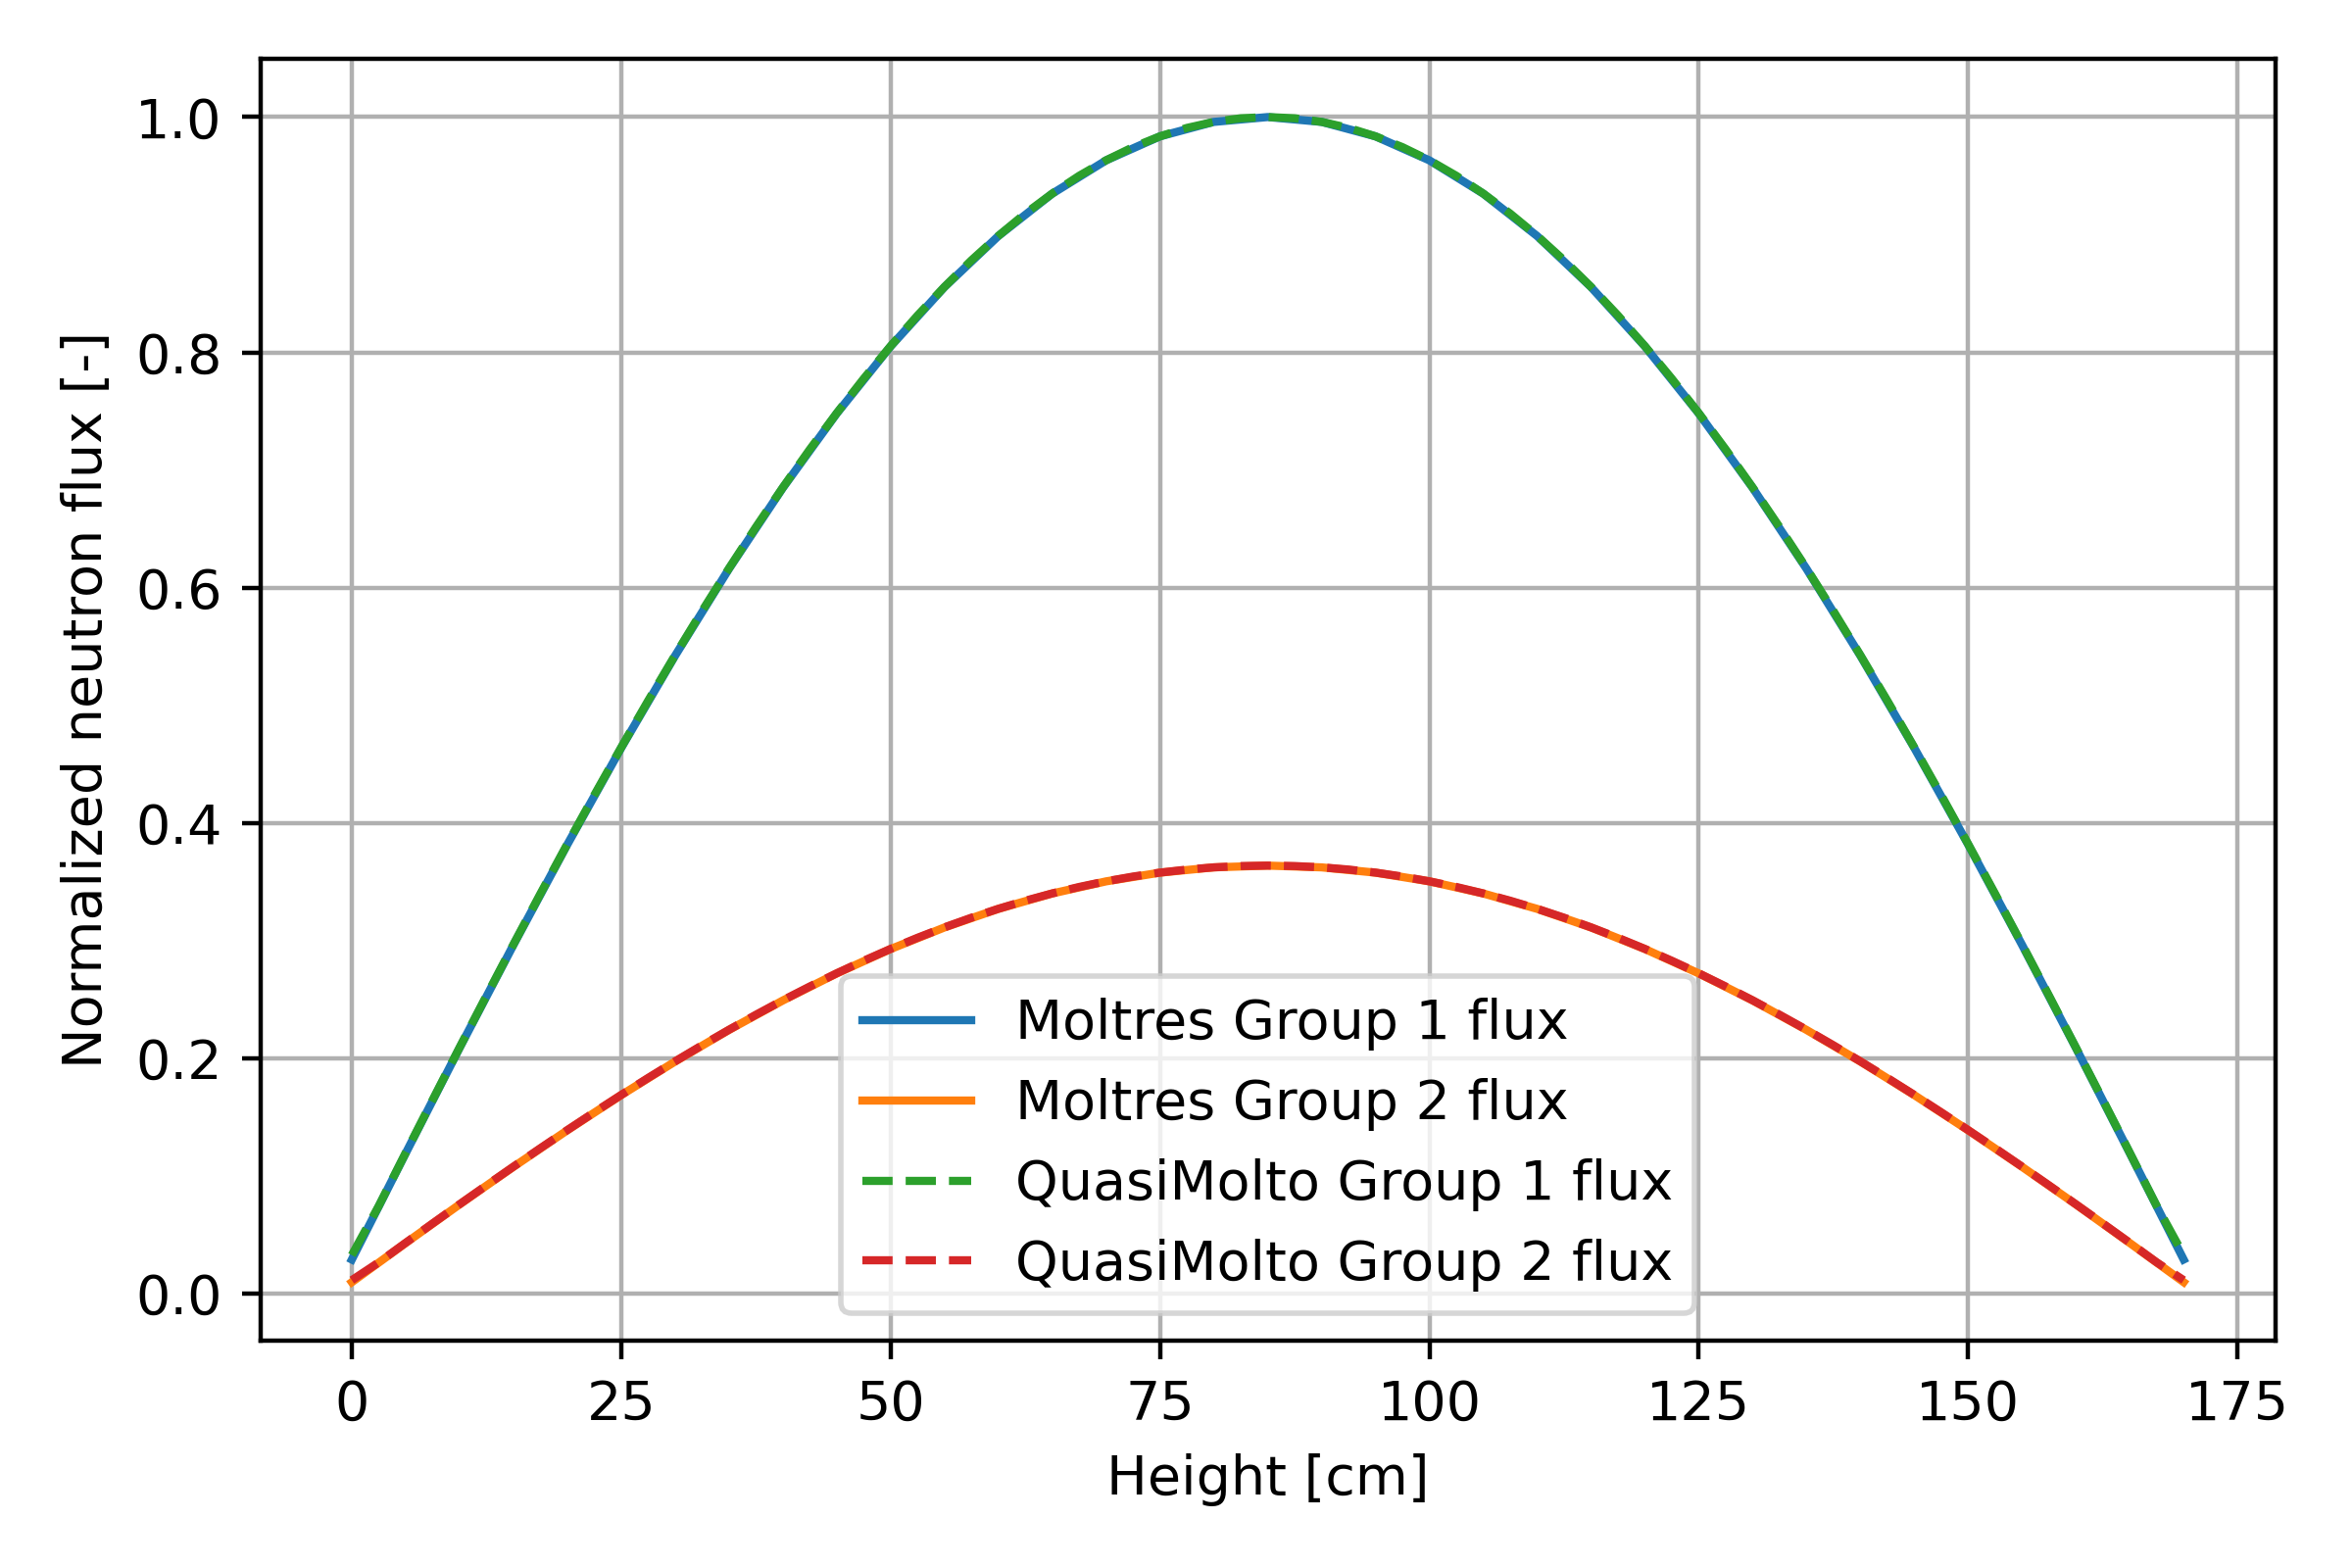
\includegraphics[width=\columnwidth]{centerline_flux}
    \caption{Normalized centerline neutron fluxes.}
    \label{fig:centerline-flux-dist}
  \end{subfigure}
  \hfill
  \begin{subfigure}[b]{0.48\columnwidth}
    \centering
    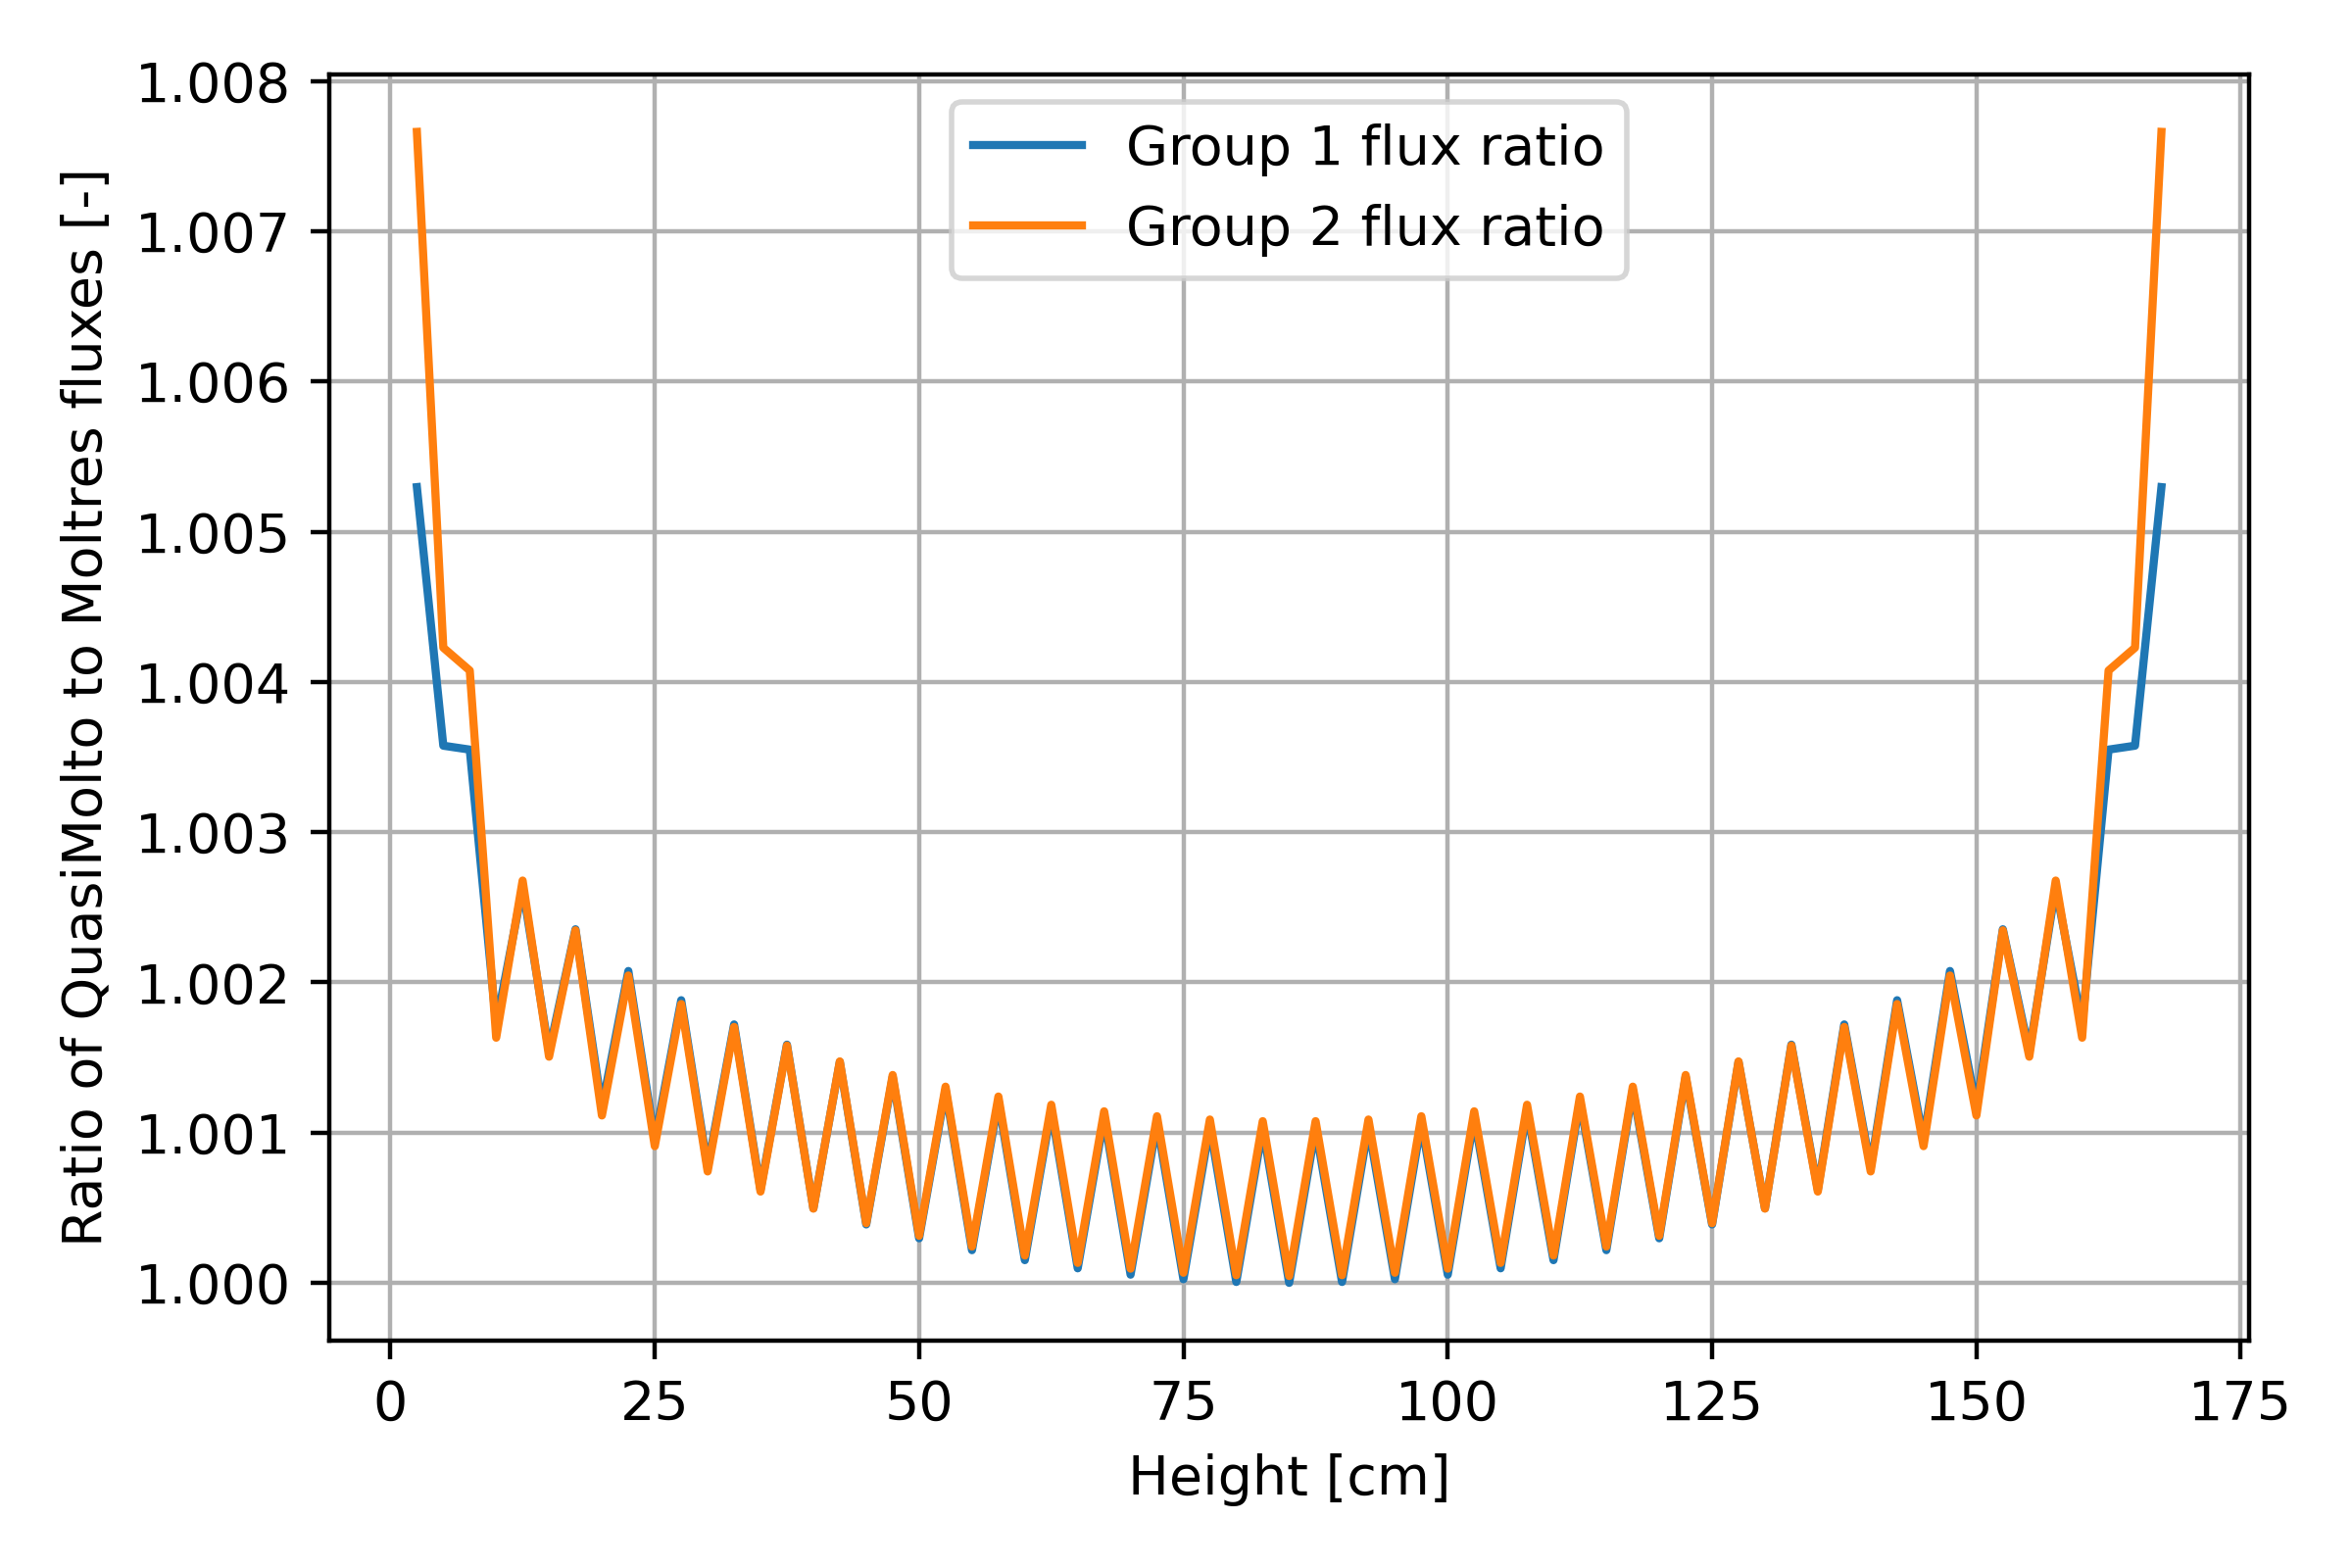
\includegraphics[width=\columnwidth]{centerline_flux_ratio}
    \caption{Ratio of centerline neutron fluxes.}
    \label{fig:centerline-flux-ratio}
  \end{subfigure}
  \caption{Centerline neutron flux distributions and ratios comparing QuasiMolto and Moltres
  \gls{MSRE} models under static conditions.}
  \label{fig:centerline-flux}
\end{figure}

\begin{figure}[htb]
  \centering
  \begin{subfigure}[b]{0.48\columnwidth}
    \centering
    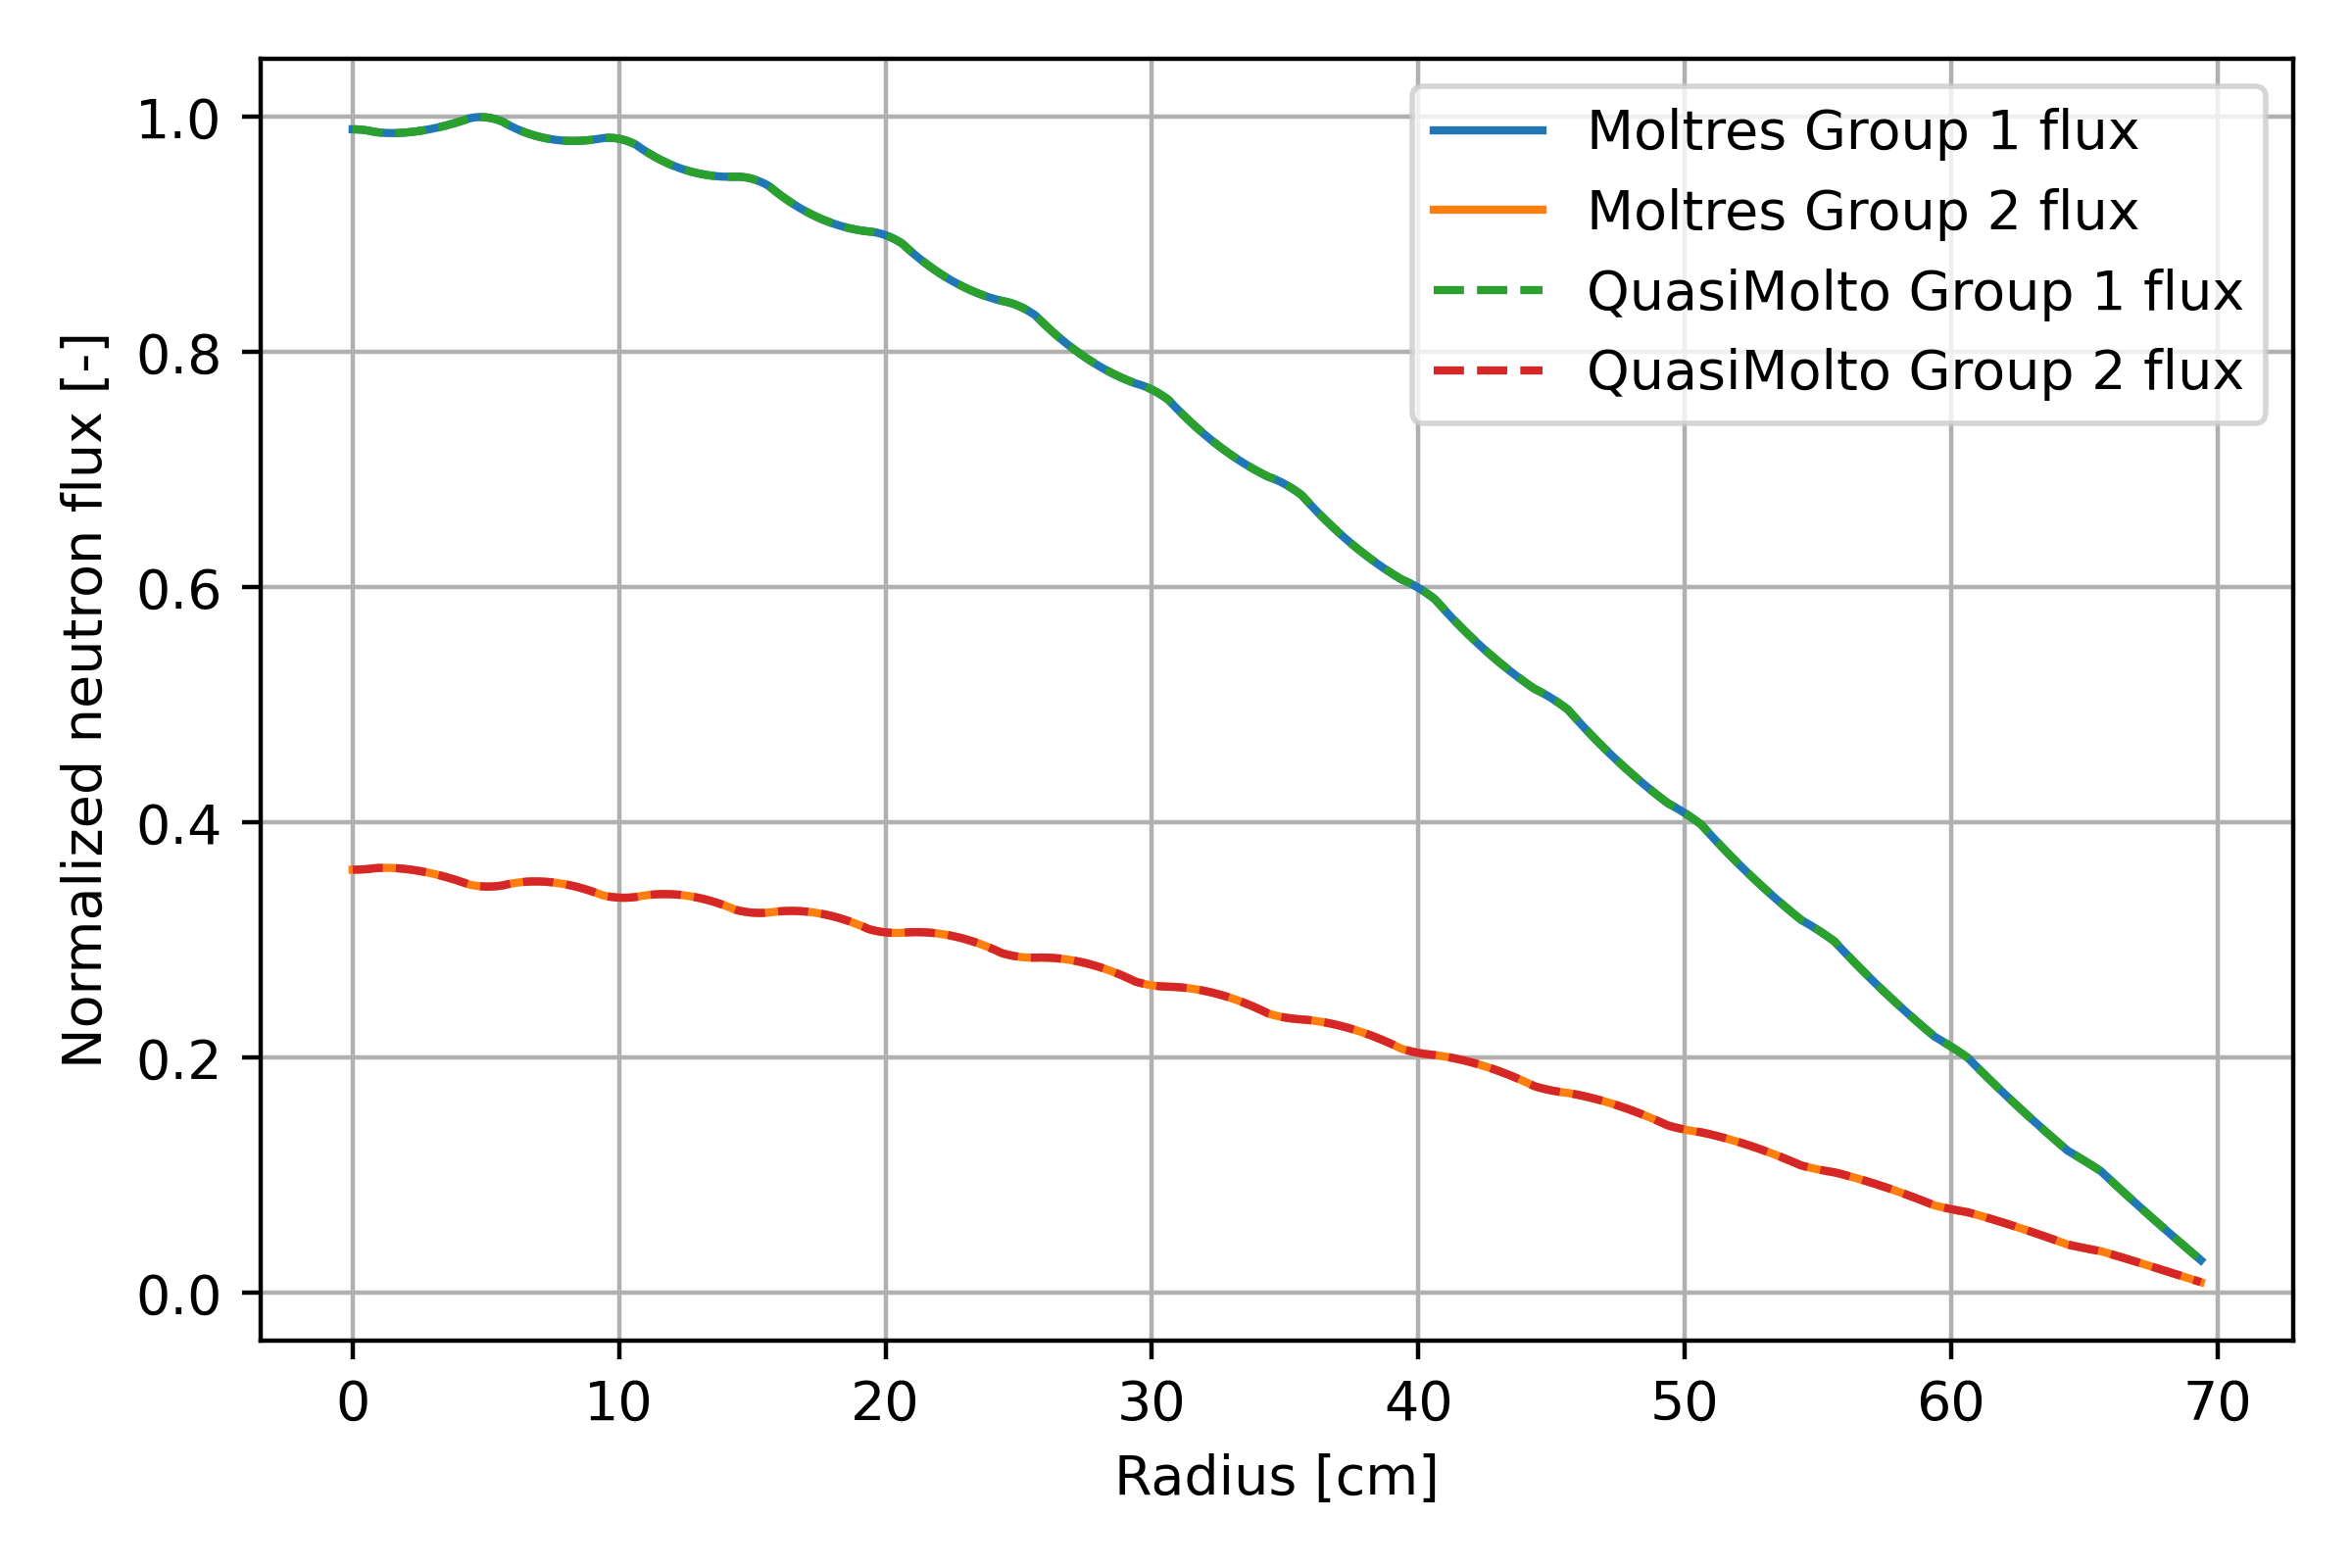
\includegraphics[width=\columnwidth]{midplane_flux}
    \caption{Normalized midplane neutron fluxes.}
    \label{fig:centerline-flux-dist}
  \end{subfigure}
  \hfill
  \begin{subfigure}[b]{0.48\columnwidth}
    \centering
    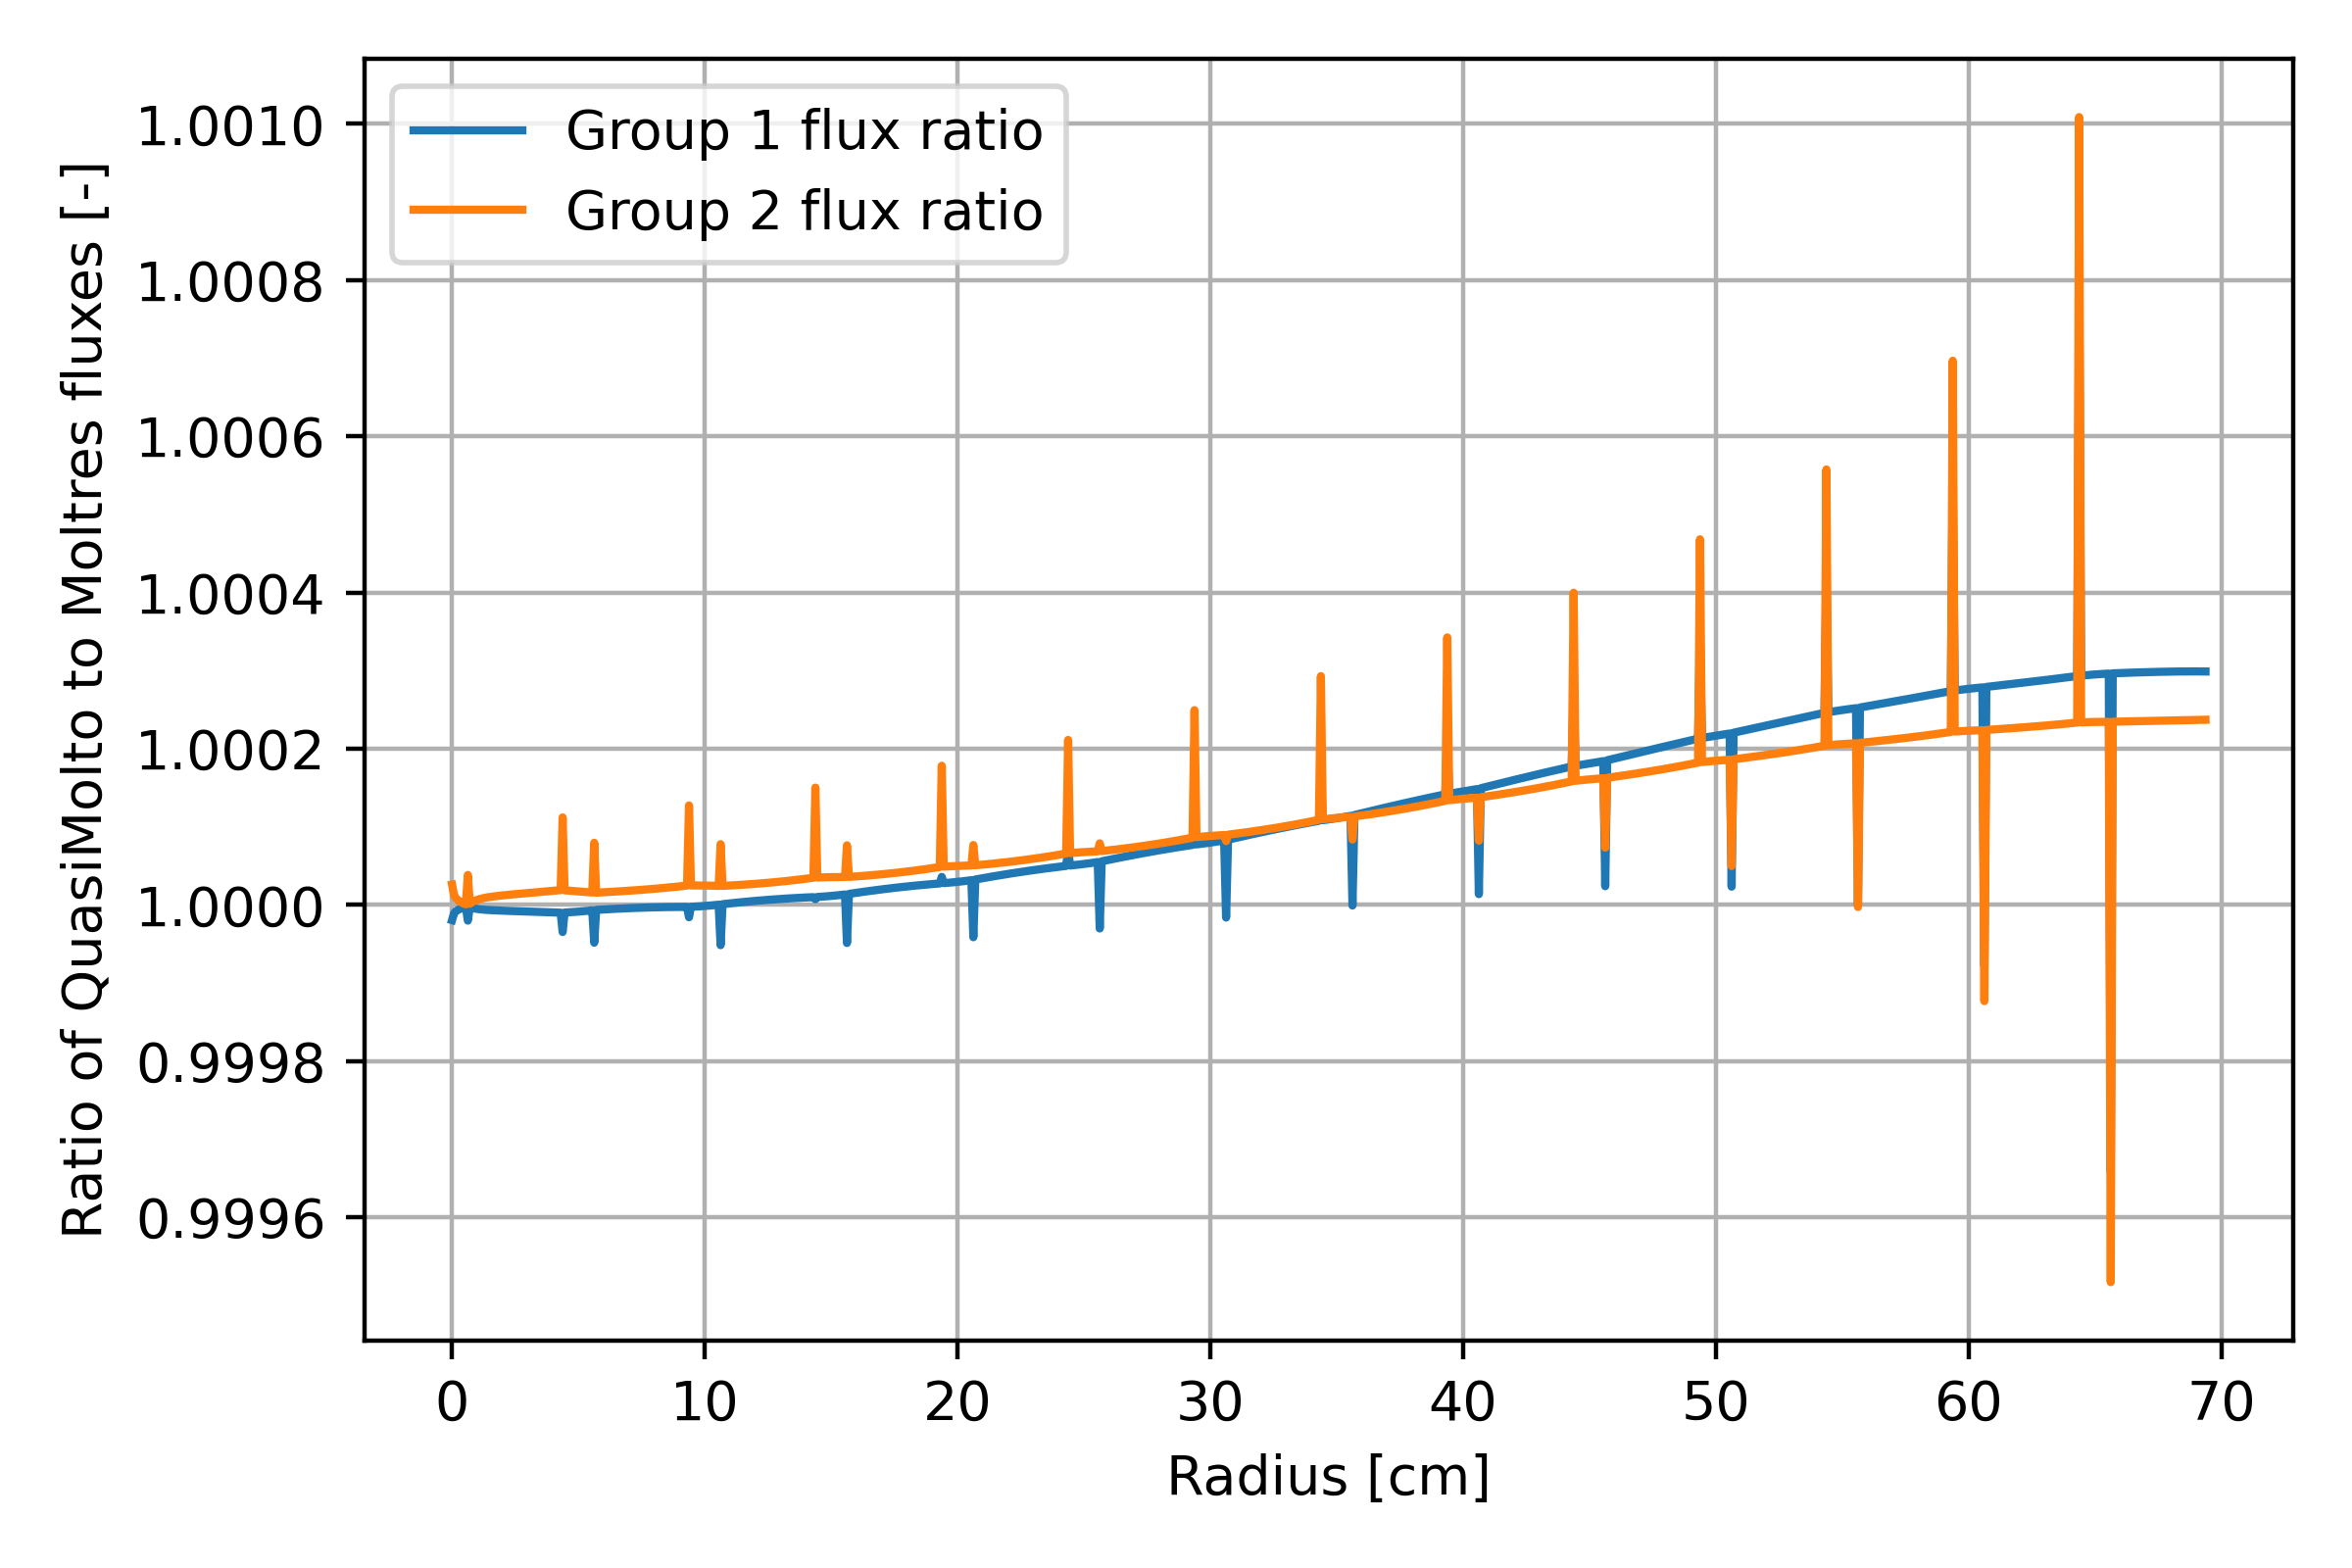
\includegraphics[width=\columnwidth]{midplane_flux_ratio}
    \caption{Ratio of midplane neutron fluxes.}
    \label{fig:centerline-flux-ratio}
  \end{subfigure}
  \caption{Midplane neutron flux distributions and ratios comparing QuasiMolto and Moltres
  \gls{MSRE} models under static conditions.}
  \label{fig:centerline-flux}
\end{figure}

\begin{figure}[htb]
  \centering
  \begin{subfigure}[b]{0.48\columnwidth}
    \centering
    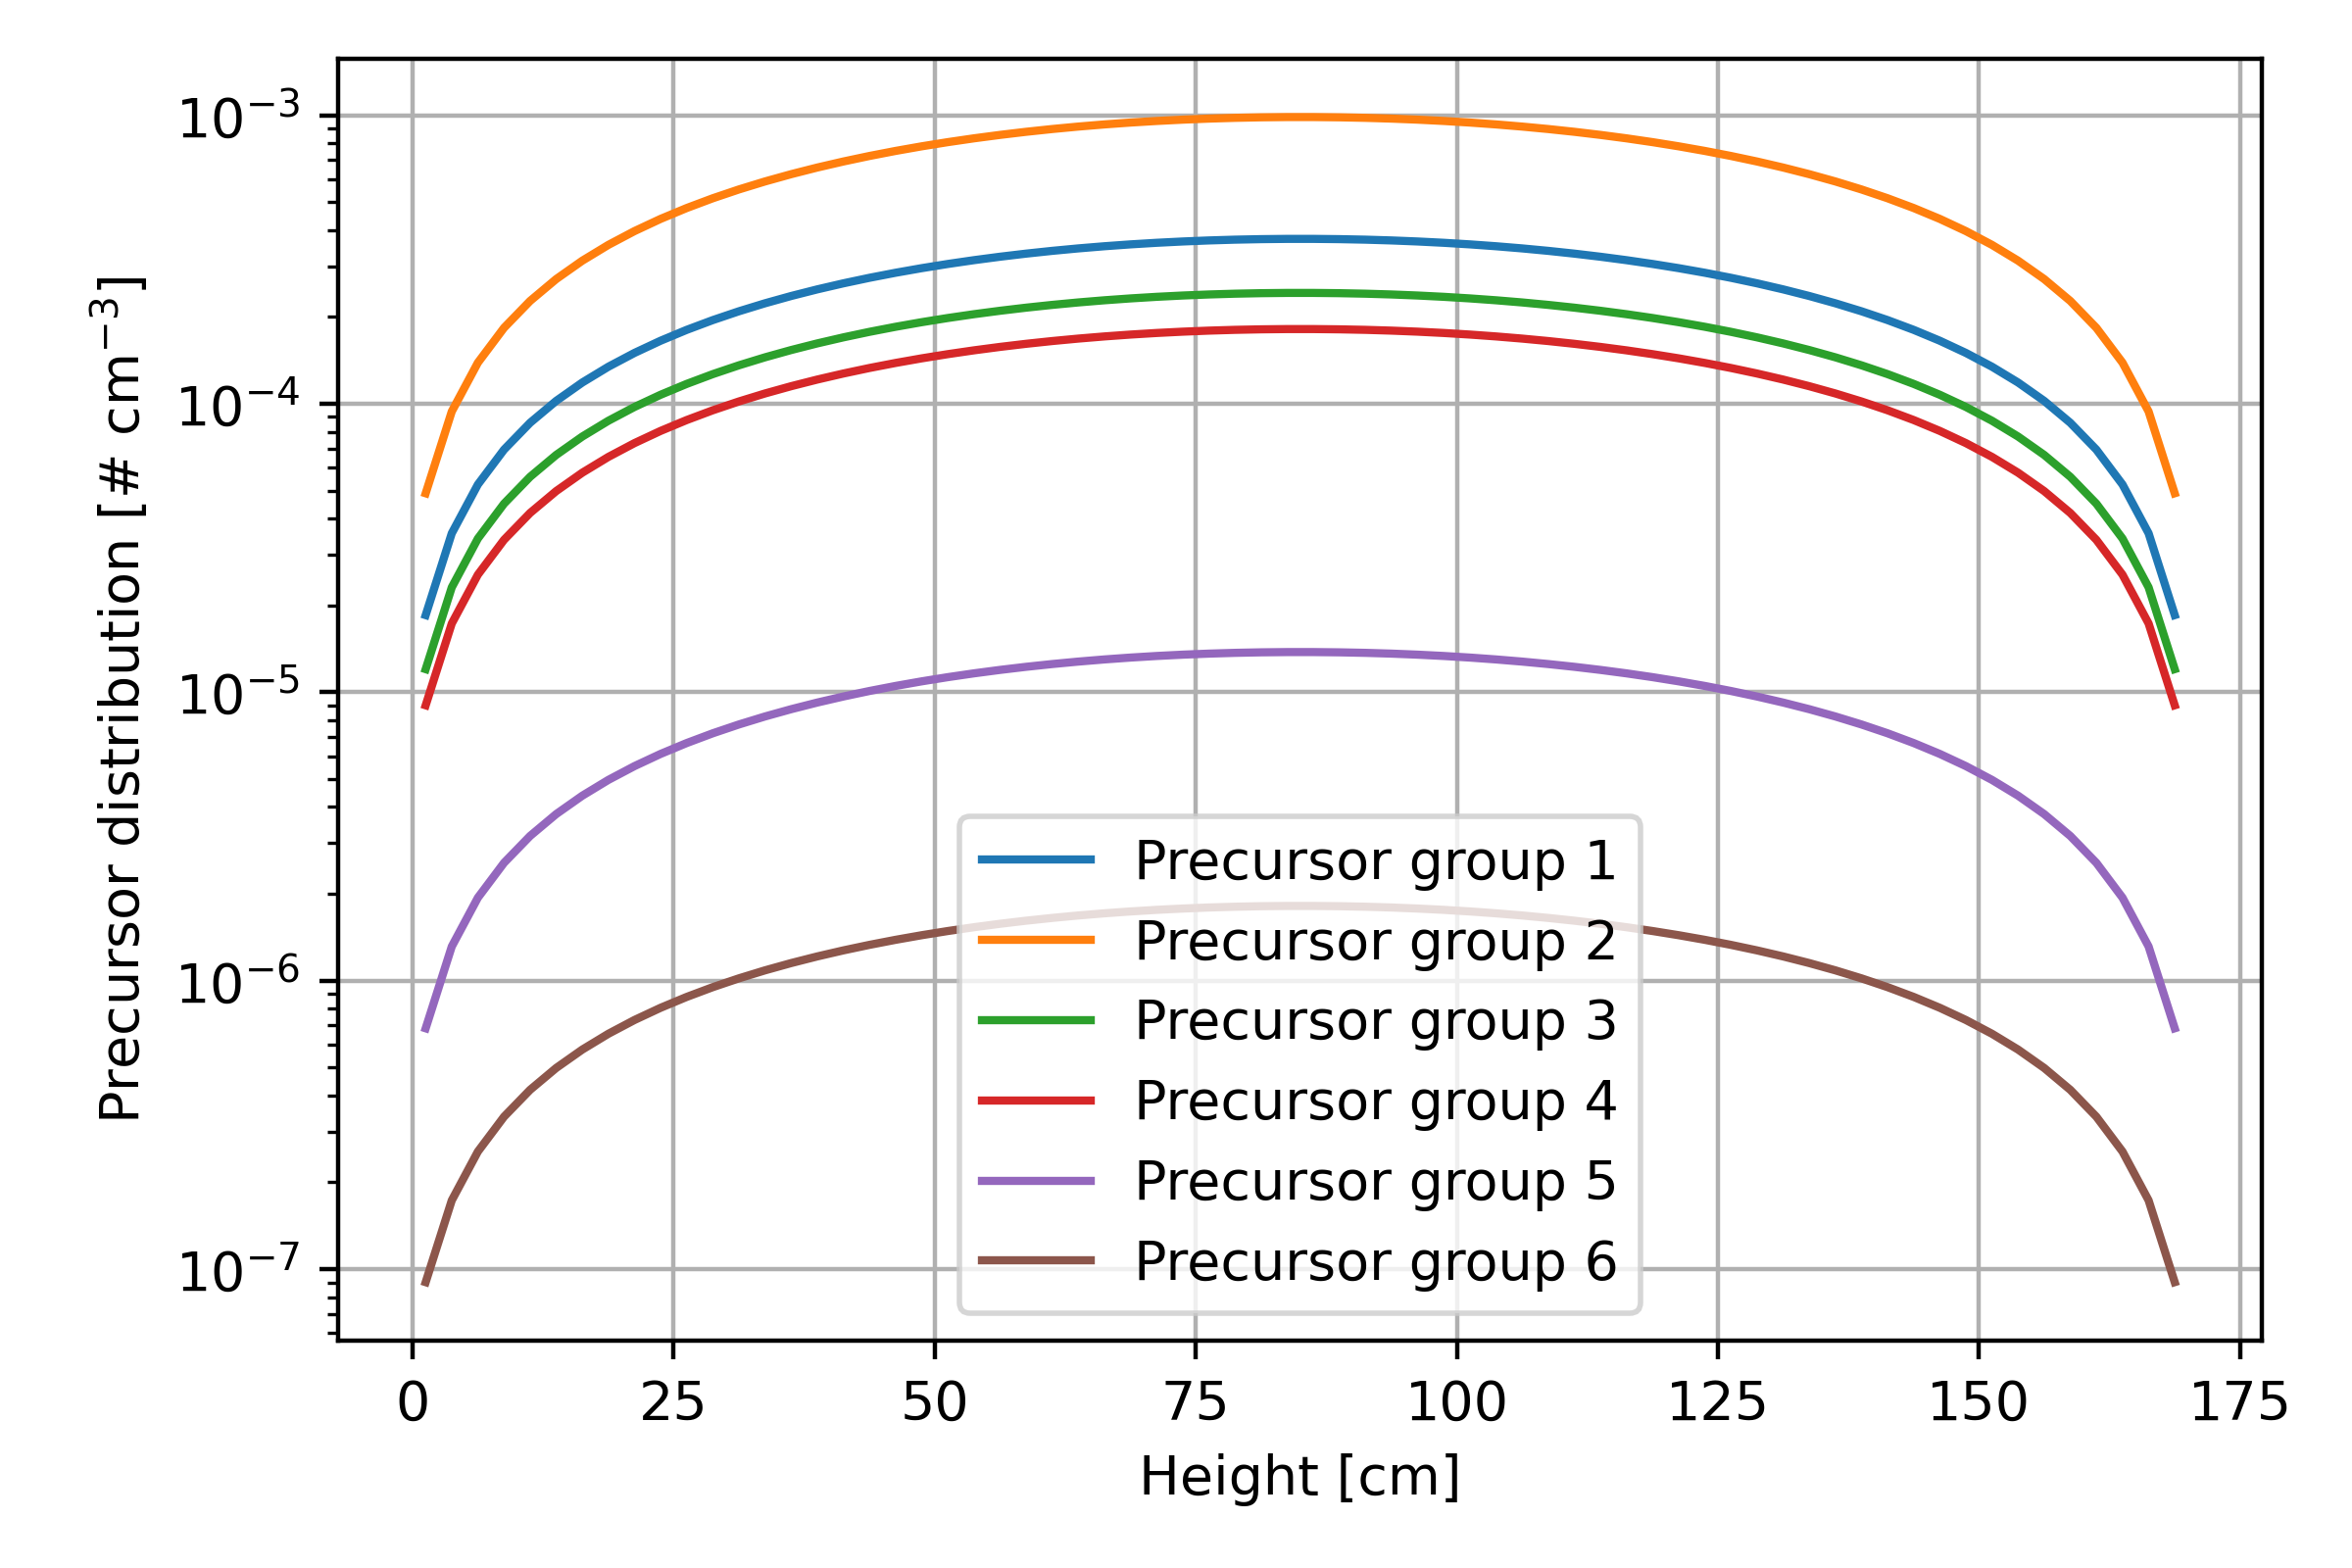
\includegraphics[width=\columnwidth]{centerline_pre}
    \caption{Normalized centerline \gls{DNP} distributions.}
    \label{fig:centerline-pre-dist}
  \end{subfigure}
  \hfill
  \begin{subfigure}[b]{0.48\columnwidth}
    \centering
    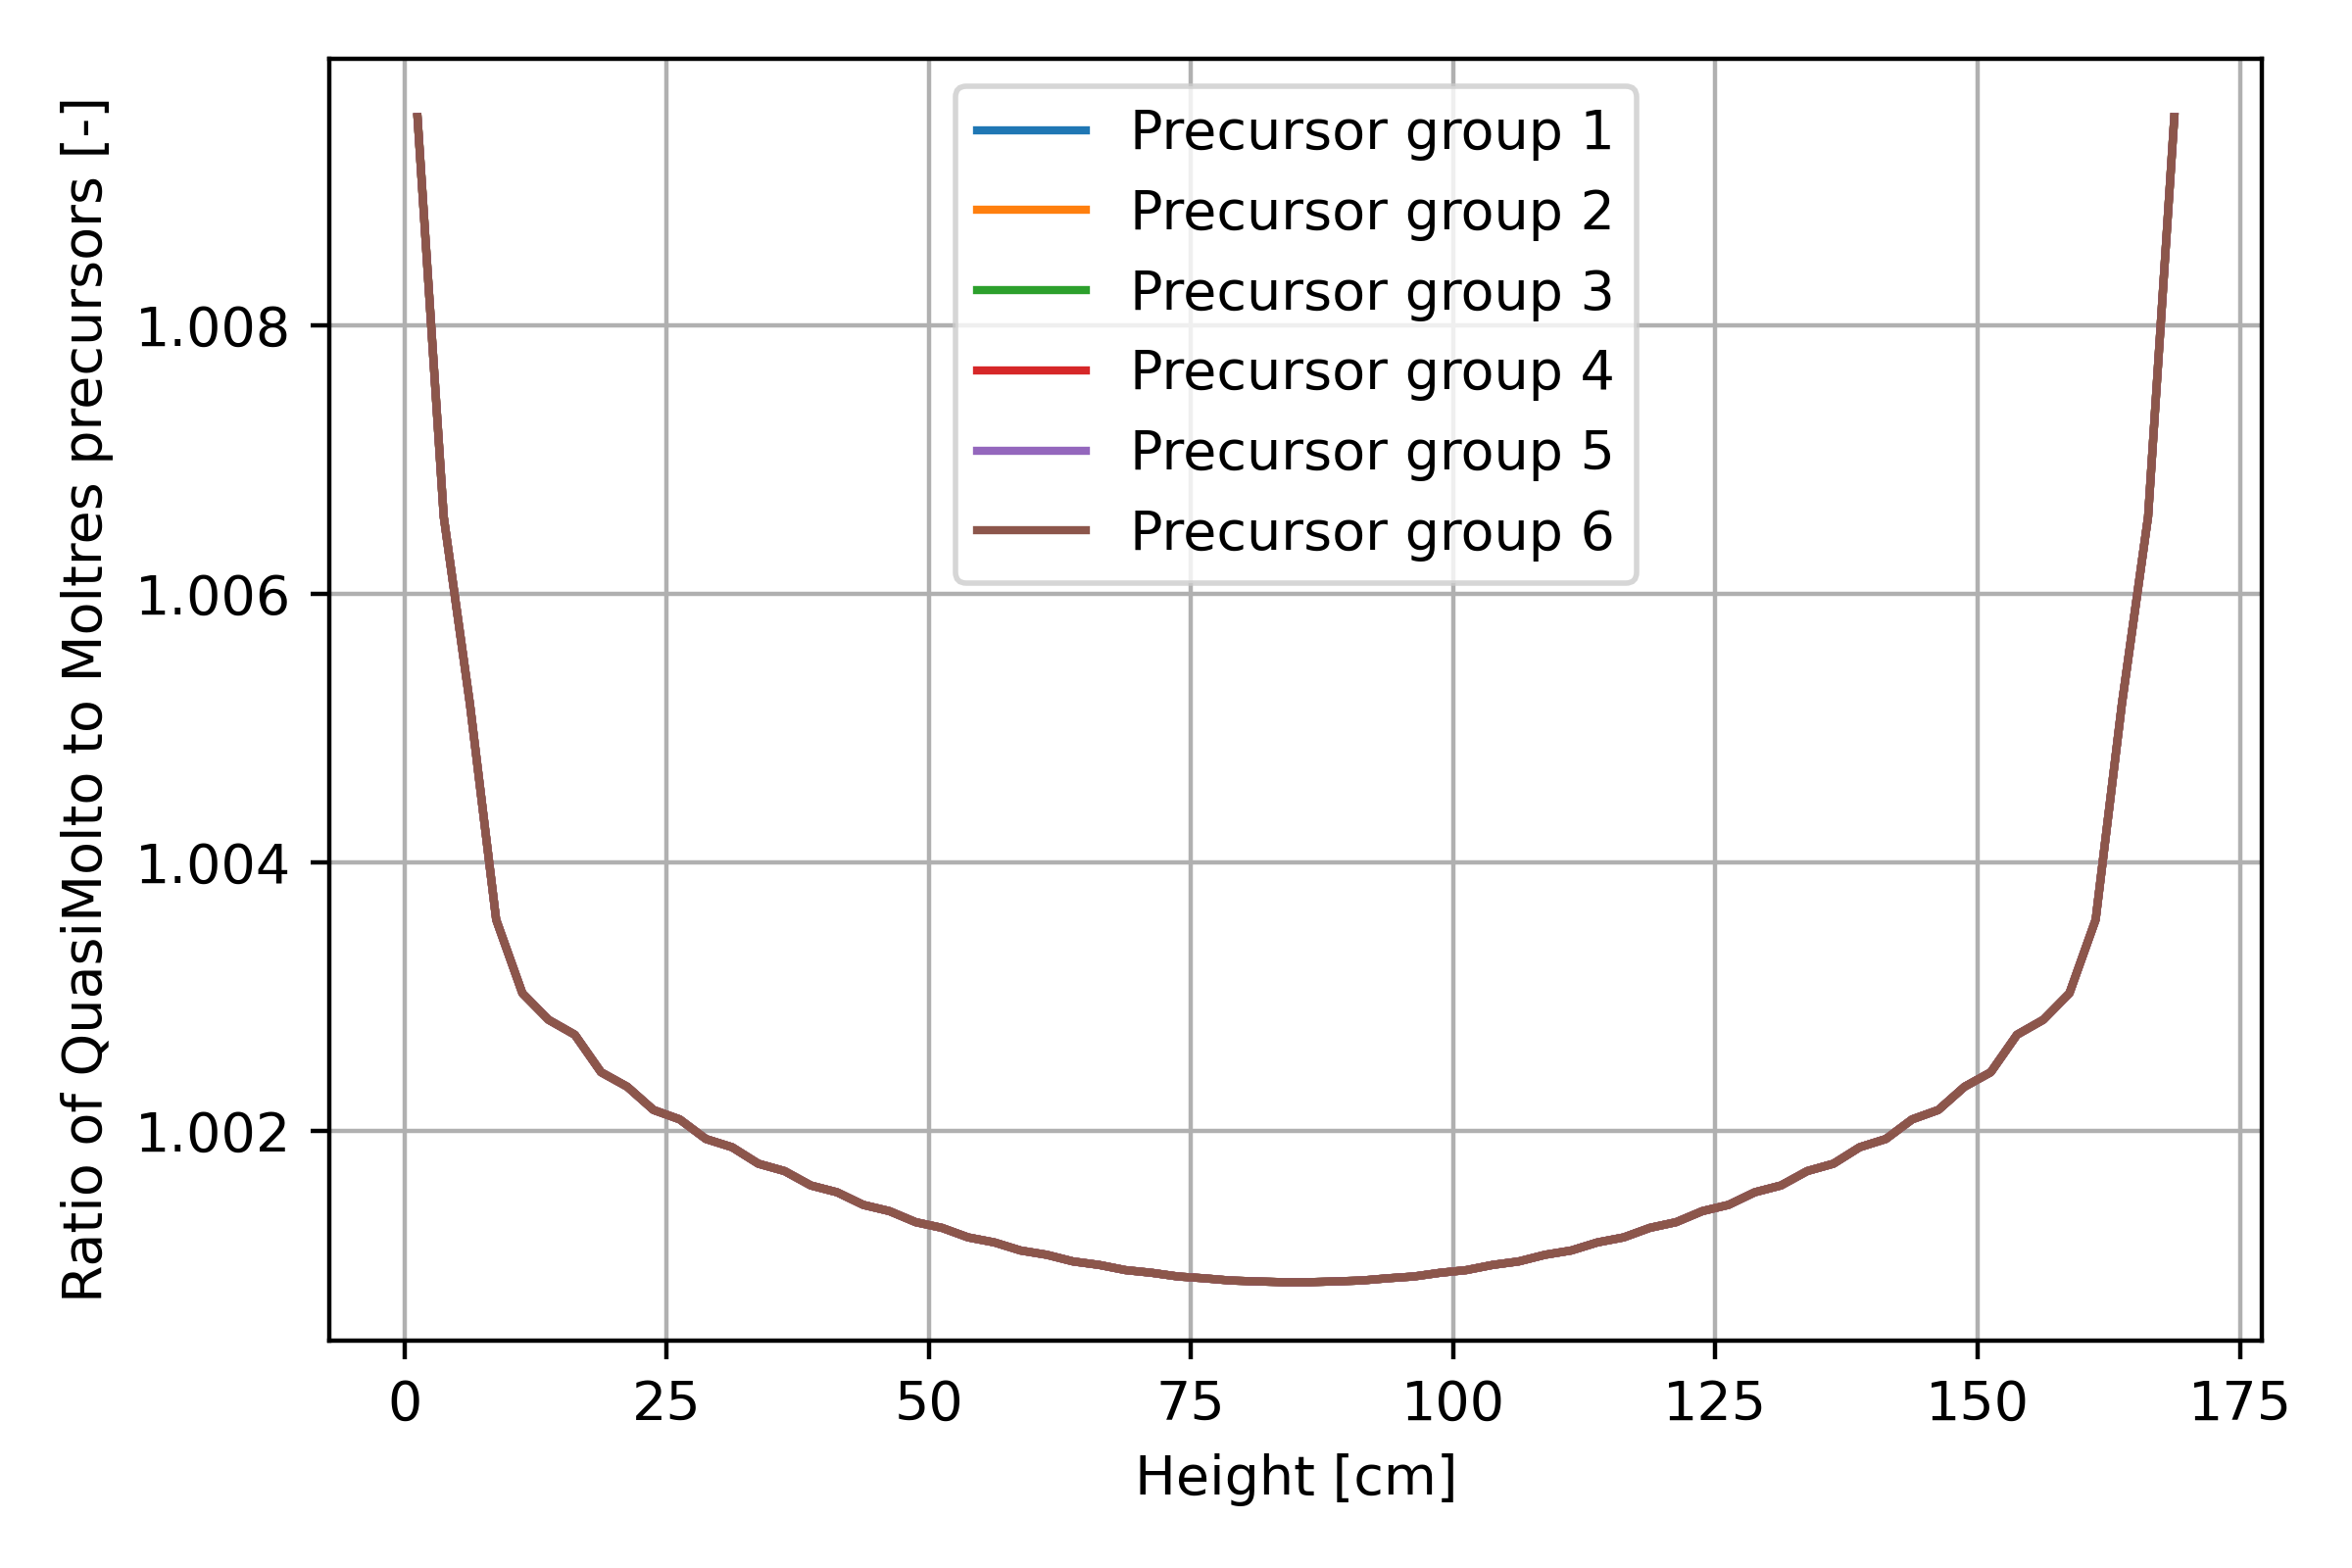
\includegraphics[width=\columnwidth]{centerline_pre_ratio}
    \caption{Ratio of centerline \gls{DNP} distributions.}
    \label{fig:centerline-pre-ratio}
  \end{subfigure}
  \caption{Centerline \gls{DNP} distribution from Moltres and ratios comparing QuasiMolto and
  Moltres models under static \gls{MSRE} conditions. The ratio curves for every \gls{DNP} group
  exhibit nearly perfect overlap.}
  \label{fig:centerline-pre}
\end{figure}

\begin{figure}[htb]
  \centering
  \begin{subfigure}[b]{0.48\columnwidth}
    \centering
    \includegraphics[width=\columnwidth]{midplane_pre}
    \caption{Normalized midplane \gls{DNP} distributions.}
    \label{fig:midplane-pre-dist}
  \end{subfigure}
  \hfill
  \begin{subfigure}[b]{0.48\columnwidth}
    \centering
    \includegraphics[width=\columnwidth]{midplane_pre_ratio}
    \caption{Ratio of midplane \gls{DNP} distributions.}
    \label{fig:midplane-pre-ratio}
  \end{subfigure}
  \caption{Midplane \gls{DNP} distribution from Moltres and ratios comparing QuasiMolto and Moltres
  models under static \gls{MSRE} conditions. \glspl{DNP} exist only in the fuel channel regions.
  The ratio curves for every \gls{DNP} group exhibit nearly perfect overlap.}
  \label{fig:midplane-pre}
\end{figure}

\begin{figure}[htb]
  \centering
  \includegraphics[width=0.9\columnwidth]{start-up-v2-reactivity}
  \caption{Reactivity (relative to static no-flow conditions) during the \gls{MSRE} pump start-up
  transient. The Moltres and QuasiMolto models agree closely with each other. The numerical models
  report greater peak and final reactivity change than the \gls{ORNL} \gls{MSRE} experimental
  data.}
  \label{fig:start-up-reactivity}
\end{figure}

\begin{figure}[htb]
  \centering
  \includegraphics[width=0.9\columnwidth]{coast-down-v2-reactivity}
  \caption{Reactivity (relative to static no-flow conditions) during the \gls{MSRE} pump coast-down
  transient. The Moltres and QuasiMolto models agree closely with each other. The numerical models
  report greater reactivity change than the \gls{ORNL} \gls{MSRE} experimental data throughout the
  transient.}
  \label{fig:coast-down-reactivity}
\end{figure}

\subsection{Summary}

\FloatBarrier


\section{Moltres Spalart-Allmaras Turbulence Model Verification} \label{sec:turbulence}

As detailed in Section \ref{sec:th}, Moltres compiles with the MOOSE Navier-Stokes
\cite{peterson_overview_2018} and Heat Transfer modules for incompressible flow
modeling capabilities by default. Moltres couples with these modules natively because they are all
built on the MOOSE framework.

To address the lack of turbulence modeling in Moltres, I implemented a Spalart-Allmaras turbulence model
\cite{spalart_one-equation_1994}, described in Section \ref{sec:lit-turb}, with \gls{SUPG}
stabilization on Moltres. The Spalart-Allmaras model estimates the turbulent eddy viscosity defined by the
eddy viscosity hypothesis applied to the \gls{RANS} equations \cite{rodi_turbulence_2017}.
On balance the Spalart-Allmaras model is a complete (does not require prior
knowledge of the actual turbulence behavior) and computationally efficient one-equation turbulence
model for approximating wall-bounded turbulent flows. The Spalart-Allmaras model implementation in Moltres
couples seamlessly with the continuous \gls{FEM} \gls{INSAD}
\cite{peterson_overview_2018, lindsay_automatic_2021} model
from the Navier-Stokes module. Alongside the Spalart-Allmaras model, Moltres also now has turbulent
diffusion physics kernels for temperature and the delayed neutron precursors.

The SA model in Moltres follows the Spalart-Allmaras model with a rotation correction scheme
\cite{aupoix_extensions_2003, dacles-mariani_numericalexperimental_1995} as described on the
\gls{NASA} Turbulence Modeling Resource website \cite{rumsey_turbulence_nodate}. The rotation
correction reduces eddy viscosity in regions of rotational but non-turbulent flow where the
original Spalart-Allmaras model overestimates eddy viscosity. The Spalart-Allmaras model implementation in Moltres
solves for the modified dynamic viscosity $\tilde{\mu}$ (as opposed to $\tilde{\nu}$) as follows:

\begin{gather}
  \rho \frac{\partial\tilde{\mu}}{\partial t} + \rho \mathbf{u}\cdot\nabla\tilde{\mu} = \rho c_{b1}
  \left(1-f_{t2}\right)\tilde{S}\tilde{\mu} + \frac{1}{\sigma}\{\nabla\cdot\left[\left(\mu+
  \tilde{\mu}\right)\nabla\tilde{\mu}\right] + c_{b2}|\nabla\tilde{\mu}|^2\} - \left(c_{w1}f_w -
  \frac{c_{b1}}{\kappa^2}f_{t2}\right)\left(
  \frac{\tilde{\mu}}{d}\right)^2
  \shortintertext{where}
  \begin{align*}
    \mu_t &= \tilde{\mu}f_{v1} = \text{turbulent eddy viscosity}, \\
    f_{v1} &= \frac{\chi^3}{\chi^3 + c_{v1}^3}, \\
    \chi &= \frac{\tilde{\mu}}{\mu}, \\
    \tilde{S} &= \Omega + \frac{\tilde{\nu}}{\kappa^2 d^2} f_{v2}, \\
    f_{v2} &= 1 - \frac{\chi}{1+\chi f_{v1}}, \\
    \Omega &= \sqrt{2W_{ij}W_{ij}} = \text{vorticity magnitude}, \\
    W_{ij} &= \frac{1}{2}\left(\frac{\partial u_i}{\partial x_j} - \frac{\partial u_j}{\partial x_i}
    \right), \\
      f_w &= g\left(\frac{1 + c_{w3}^6}{g^6 + c_{w3}^6}\right)^{1/6}, \\
      g &= r + c_{w2}\left(r^6 - r\right), \\
      r &= \text{min}\left(\frac{\tilde{\nu}}{\tilde{S}\kappa^2d^2}, 10\right), \\
      f_{t2} &= c_{t3} \exp{\left(-c_{t4}\chi^2\right)},
  \end{align*}
\shortintertext{and the constants are}
  \sigma = \frac{2}{3}, \ c_{b1} = 0.1355, \ c_{b2} = 0.622, \ \kappa = 0.41, \
  c_{w1} = \frac{c_{b1}}{\kappa^2} + \frac{1+c_{b2}}{\sigma}, \nonumber \\
  c_{w2} = 0.3, \ c_{w3} = 2, \
  c_{v1} = 7.1, \ c_{t3} = 1.2, \ c_{t4} = 0.5 \ \text{.} \nonumber
\end{gather}

The $f_{t2}$ turbulence trip term is togglable using the \texttt{use\_ft2\_term} input parameter
(false by default) if turbulence trip (initiation) is not necessary
\cite{rumsey_turbulence_nodate}. The following subsections cover verification and validation tests
of the Spalart-Allmaras model in Moltres using reference problems for turbulent channel, pipe, and
\gls{BFS} flow. Moltres input files
for all three reference problems are available at
\url{https://github.com/arfc/moltres/tree/devel/problems/2023-basic-turbulence-cases}.
The Moltres test dataset is available on Zenodo at this reference listing \cite{park_dataset_2023}.

\subsection{Turbulent Channel Flow Verification Test}

Moser et al.\ \cite{moser_direct_1999} performed \gls{DNS} simulations of turbulent channel flow
for friction Reynolds number, Re$_\tau\approx395$ (corresponds to Reynolds number, Re
$\approx 13750$). Their results serve as the reference solution for this turbulent channel flow
test.

The Moltres model for this test is a 2-D 140 m$\times$0.5 m half-channel
(Figure \ref{fig:channel-geom}). The main flow direction
is in the positive $x$ direction with the inlet and outlet on the left and right ends,
respectively. The channel wall lies along the top boundary ($y=0.5$ m) while the bottom boundary
($y=0$ m) serves as a symmetry axis for the half-channel geometry. Figure \ref{fig:channel-mesh}
shows a close-up view of the refined mesh near the inlet and along the top wall boundary. The mesh
for the rest of the channel geometry follows the same mesh resolution as the rightmost column of
elements shown on the right side of Figure \ref{fig:channel-mesh}. The dimensionless wall distance
parameter $y^+$ of the first mesh element along wall boundary for fully developed flow at the end
of the channel is 0.974, meeting the
$y^+ \lesssim 1$ requirement for properly wall-resolved flow. Table \ref{table:channel} lists
relevant flow parameters for the turbulent channel flow test. The Moltres channel flow model
ran as a time-dependent simulation with adaptive time-stepping starting from a timestep size of 0.1
s up to a maximum timestep size of 10 s with a timestep size growth factor of 1.1. The simulation
automatically terminated at $t=186$ s when Moltres detected that the flow profile reached
steady-state, i.e., the flow and turbulent viscosity distributions remained unchanged between
successive timesteps.

\begin{figure}[p]
  \centering
  \includegraphics[width=0.9\columnwidth]{channel-geom}
  \caption{Channel geometry for the turbulent channel flow verification test. The red box indicates
  the region shown by the close-up view in Figure \ref{fig:channel-mesh}.}
  \label{fig:channel-geom}
%\end{figure}
%%
%\begin{figure}[htb!]
  \centering
  \includegraphics[width=\columnwidth]{channel_mesh}
  \caption{Close-up view of the refined mesh near the inlet (left boundary) for the channel flow
    test. The mesh for the rest of the channel follows the mesh resolution of the rightmost column
  of elements.}
  \label{fig:channel-mesh}
\end{figure}

\begin{table}[htb]
  \centering
  \small
  \caption{Relevant turbulent channel flow problem parameters. The $\tilde{\mu}_\text{inlet}$ value
  at the inlet is set to fives times the $\mu$ value as recommended for the Spalart-Allmaras model
  \cite{spalart_one-equation_1994}.}
  \begin{tabular}{l S}
    \toprule
    Property & {Value} \\
    \midrule
    Density, $\rho$ [kg m$^{-3}$] & 1.0 \\
    Inlet velocity, $v_x$ [m s$^{-1}$] & 1.0 \\
    Dynamic viscosity, $\mu$ [kg m$^{-1}$ s$^{-1}$] & 7.272e-5 \\
    Reynolds number, Re [-] & 1.375e4 \\
    Modified viscosity along inlet, $\tilde{\mu}_\text{inlet}$ [kg m$^{-1}$ s$^{-1}$] & 3.636e-4 \\
    Modified viscosity along wall, $\tilde{\mu}_\text{wall}$ [kg m$^{-1}$ s$^{-1}$] & 0.0 \\
    \bottomrule
  \end{tabular}
  \label{table:channel}
\end{table}

Figure \ref{fig:channel-verification} shows plots of normalized and nondimensionalized velocities,
wall distances, and stresses from the \gls{DNS} data \cite{moser_direct_1999}
and the Moltres Spalart-Allmaras model. The Moltres Spalart-Allmaras model is largely consistent with the reference
\gls{DNS} flow data and reproduces the expected trends in the velocity and stress distributions
across the channel and as a function of the wall distance.

\begin{figure}[htb!]
  \centering
  \begin{subfigure}[b]{0.48\columnwidth}
    \centering
    \includegraphics[width=\columnwidth]{channel_vel}
    \caption{Normalized velocity distribution across the channel.}
    \label{fig:channel-vel}
  \end{subfigure}
  \hfill
  \begin{subfigure}[b]{0.48\columnwidth}
    \centering
    \includegraphics[width=\columnwidth]{channel_nondim}
    \caption{Dimensionless velocity vs.\ dimensionless wall distance.}
    \label{fig:channel-nondim}
  \end{subfigure}
  \begin{subfigure}[b]{0.48\columnwidth}
    \centering
    \includegraphics[width=\columnwidth]{channel_stress}
    \caption{Normalized stress distribution across the channel.}
    \label{fig:channel-stress}
  \end{subfigure}
  \caption{Comparison of turbulent channel flow results at Re$_\tau\approx395$ against reference
  \gls{DNS} results \cite{moser_direct_1999}. The Moltres Spalart-Allmaras model agrees consistently with
  the reference data.}
  \label{fig:channel-verification}
\end{figure}

\subsection{Turbulent Pipe Flow Validation Test}

In 1954, Laufer performed turbulent pipe flow experiments for Re $\approx 40000$
\cite{laufer_structure_1954}. Their results serve as the reference solution for this turbulent pipe
flow test.

\begin{figure}[p]
  \centering
  \includegraphics[width=0.8\columnwidth]{pipe-geom}
  \caption{Pipe geometry for the turbulent pipe flow verification test. The red box indicates
  the region shown by the close-up views in Figure \ref{fig:pipe-mesh}.}
  \label{fig:pipe-geom}
%\end{figure}
%%
%\begin{figure}[htb!]
  \centering
  \begin{subfigure}[b]{0.40\columnwidth}
    \centering
    \includegraphics[width=\columnwidth]{pipe_mesh}
    \caption{Close-up view of the refined mesh near the inlet for the pipe flow test.}
    \label{fig:pipe-mesh-1}
  \end{subfigure}
  \hfill
  \begin{subfigure}[b]{0.53\columnwidth}
    \centering
    \includegraphics[width=\columnwidth]{pipe_mesh_zoom}
    \caption{Close-up view of the refined mesh near the inlet and wall boundary interface.}
    \label{fig:pipe-mesh-2}
  \end{subfigure}
  \caption{Close-up views of the refined mesh near the inlet (bottom boundary) and wall (right
  boundary). The mesh for the rest of the channel follows the mesh resolution of the topmost row of
  elements in the left subfigure.}
  \label{fig:pipe-mesh}
\end{figure}

The Moltres model for this test is a 2-D axisymmetric (R-Z coordinates) half-pipe with a radius of
0.5 m and a length of 150 m (Figure \ref{fig:pipe-geom}). The main flow direction
is in the positive $z$ direction with the inlet and outlet on the bottom and top ends,
respectively. The channel wall lies along the right boundary ($r=0.5$ m) while the left boundary
($r=0$ m) serves as a symmetry axis for the half-pipe geometry. Figure \ref{fig:pipe-mesh} shows
two close-up views of the refined mesh near the inlet and along the right wall boundary. The mesh
for the rest of the pipe geometry follows the same mesh resolution as the topmost row of
elements shown on the near the top of Figure \ref{fig:pipe-mesh-1}. The dimensionless wall distance
parameter $y^+$ of the first mesh element along wall boundary for fully developed flow at the end
of the pipe is 0.847, meeting the
$y^+ \lesssim 1$ requirement for properly wall-resolved flow. Table \ref{table:channel} lists
relevant flow parameters for the turbulent pipe flow test. The Moltres channel flow model ran as a
time-dependent simulation with adaptive time-stepping starting from a timestep size of 0.01
s up to a maximum timestep size of 10 s with a timestep size growth factor of 1.1. The simulation
automatically terminated at $t=165$ s when Moltres detected that the flow profile reached
steady-state, i.e., the flow and turbulent viscosity distributions remained unchanged between
successive timesteps.

\begin{table}[htb]
  \centering
  \small
  \caption{Relevant turbulent pipe flow problem parameters. The $\tilde{\mu}_\text{inlet}$ value
  at the inlet is set to fives times the $\mu$ value as recommended for the Spalart-Allmaras model
  \cite{spalart_one-equation_1994}.}
  \begin{tabular}{l S}
    \toprule
    Property & {Value} \\
    \midrule
    Density, $\rho$ [kg m$^{-3}$] & 1.0 \\
    Inlet velocity, $v_z$ [m s$^{-1}$] & 1.0 \\
    Dynamic viscosity, $\mu$ [kg m$^{-1}$ s$^{-1}$] & 2.5e-5 \\
    Reynolds number, Re [-] & 4.0e4 \\
    Modified viscosity along inlet, $\tilde{\mu}_\text{inlet}$ [kg m$^{-1}$ s$^{-1}$] & 1.25e-4 \\
    Modified viscosity along wall, $\tilde{\mu}_\text{wall}$ [kg m$^{-1}$ s$^{-1}$] & 0.0 \\
    \bottomrule
  \end{tabular}
  \label{table:pipe}
\end{table}

Figure \ref{fig:pipe-verification} shows plots of normalized and nondimensionalized velocities,
wall distances, and stresses from the experimental data \cite{laufer_structure_1954}
and the Moltres Spalart-Allmaras model. The Moltres Spalart-Allmaras model is largely consistent with the reference
experimental flow data and reproduces the expected trends in the velocity and stress distributions
across the channel and as a function of the wall distance.

\begin{figure}[htb]
  \centering
  \begin{subfigure}[b]{0.48\columnwidth}
    \centering
    \includegraphics[width=\columnwidth]{pipe_vel}
    \caption{Normalized velocity distribution across the pipe.}
    \label{fig:pipe-vel}
  \end{subfigure}
  \hfill
  \begin{subfigure}[b]{0.48\columnwidth}
    \centering
    \includegraphics[width=\columnwidth]{pipe_nondim}
    \caption{Dimensionless velocity vs.\ dimensionless wall distance}
    \label{fig:pipe-nondim}
  \end{subfigure}
  \begin{subfigure}[b]{0.48\columnwidth}
    \centering
    \includegraphics[width=\columnwidth]{pipe_stress}
    \caption{Normalized turbulent shear stress distribution across the pipe.}
    \label{fig:pipe-stress}
  \end{subfigure}
  \caption{Comparison of turbulent pipe flow results at Re $\approx 40000$ against reference
  experimental data \cite{laufer_structure_1954}.}
  \label{fig:pipe-verification}
\end{figure}

\FloatBarrier

\subsection{Backward-Facing Step Flow Validation Test}

Driver \& Seegmiller performed the \gls{BFS} flow experiment for Re $\approx36000$ (based on the
step height)
\cite{driver_features_1985}. Their results serve as the reference solution for this \gls{BFS} test.
Additionally, the \gls{NASA} Turbulence Modeling Resource website \cite{rumsey_turbulence_nodate}
provides \gls{BFS} simulation results generated from the regular Spalart-Allmaras model in the CFL3D
Navier-Stokes CFD code developed at \gls{NASA} \cite{krist_cfl3d_1998}. The CFL3D Spalart-Allmaras model
does not contain the rotation correction scheme
\cite{aupoix_extensions_2003, dacles-mariani_numericalexperimental_1995} present in the Moltres
Spalart-Allmaras model.

\begin{figure}[p]
  \centering
  \includegraphics[width=0.9\columnwidth]{backstep-geom}
  \caption{Backward step geometry for the turbulent \gls{BFS} flow verification test. The red box indicates
  the region shown by the close-up view in Figure \ref{fig:bfs-mesh}.}
  \label{fig:backstep-geom}
%\begin{figure}[htb!]
  \centering
  \includegraphics[width=0.9\columnwidth]{bfs_mesh}
  \caption{Close-up view of the mesh for the \gls{BFS} flow test. The step is situated at $x=110$ m
  with a height of $H=1$ m.}
  \label{fig:bfs-mesh}
\end{figure}

The Moltres model for this test is a 2-D 160 m-long channel (Figure \ref{fig:backstep-geom}.
The main flow direction is in the
positive $x$ direction with the inlet and outlet on the left and right ends, respectively. The
channel is 8 m tall before the 1 m-tall step at $x=110$ m. Figure \ref{fig:bfs-mesh} shows a
close-up view of the mesh around the step. The dimensionless wall distance parameter $y^+$ of the
first mesh elements along wall boundaries just prior to the step and at the end of the channel are
0.735 and 0.555, respectively, meeting the $y^+ \lesssim 1$ requirement for properly wall-resolved
flow. Table \ref{table:bfs} lists relevant flow parameters for the turbulent \gls{BFS} flow test.
The Moltres \gls{BFS} flow model ran as two separate simulations for the upstream turbulent flow
profile to fully develop from $x=0$ m to $x=104$ m and the \gls{BFS} flow profile from $x=104$ m to
$x=160$ m. The fully-developed flow profile at $x=104$ m from the first simulation served as the
inlet flow profile for the second simulation. Both simulations ran with adaptive time-stepping
starting from a timestep size of 0.1 s up to a maximum timestep size of 10 s with a timestep size
growth factor of 1.1. The upstream and \gls{BFS} simulations automatically terminated at $t=212$ s
and $t=223$ s when Moltres detected that the flow profiles reached steady-state.

\begin{table}[htb]
  \centering
  \small
  \caption{Relevant turbulent \gls{BFS} flow problem parameters. The $\tilde{\mu}_\text{inlet}$ value
  at the inlet is set to fives times the $\mu$ value as recommended for the Spalart-Allmaras model
  \cite{spalart_one-equation_1994}.}
  \begin{tabular}{l S}
    \toprule
    Property & {Value} \\
    \midrule
    Density, $\rho$ [kg m$^{-3}$] & 1.0 \\
    Inlet velocity, $v_z$ [m s$^{-1}$] & 1.0 \\
    Dynamic viscosity, $\mu$ [kg m$^{-1}$ s$^{-1}$] & 2.778e-5 \\
    Reynolds number based on step height $H=1$ m, Re$_H$ [-] & 3.6e4 \\
    Modified viscosity along inlet, $\tilde{\mu}_\text{inlet}$ [kg m$^{-1}$ s$^{-1}$] & 1.389e-4 \\
    Modified viscosity along wall, $\tilde{\mu}_\text{wall}$ [kg m$^{-1}$ s$^{-1}$] & 0.0 \\
    \bottomrule
  \end{tabular}
  \label{table:bfs}
\end{table}

Figure \ref{fig:bfs} shows the velocity magnitude and streamlines around the step at $x=110$ m. The
streamlines illustrate the recirculation zones created by flow separation past the step.
Figure \ref{fig:bfs-plots} shows the normalized velocity distributions at various distances from
step, the skin friction and skin pressure coefficients along the bottom wall, and the normalized
turbulent shear stress distributions at various distances downstream of the step. The Spalart-Allmaras
model with the rotation correction scheme in Moltres performs largely similarly to the reference
Spalart-Allmaras model results provided on the \gls{NASA} Turbulence Modeling Resource website
\cite{rumsey_turbulence_nodate}. Compared with the reference experimental data, the Moltres
Spalart-Allmaras model predicts more accurate velocity (Figure \ref{fig:bfs-downstream}) and turbulent
stress distributions (Figure \ref{fig:bfs-stress}) along $x/H=1$ downstream of the
step than the CFL3D Spalart-Allmaras model. This indicates that the Moltres
Spalart-Allmaras model reproduces the sizes and shapes of the largest and second-largest recirculation
zones (see Figure \ref{fig:bfs}) more accurately than the CFL3D Spalart-Allmaras model. Table
\ref{table:bfs-reattach} further supports the prior observation since the flow reattachment length
estimate from Moltres is more consistent with the experimental data than CFL3D. The Moltres
Spalart-Allmaras velocity distributions in Figure \ref{fig:bfs-downstream} are largely consistent with the
experimental data. Lastly, the reader should
note that this turbulent \gls{BFS} flow setup induces complex flow separation effects despite the
apparent simplicity of the geometry. All \gls{RANS}-based model results from the \gls{NASA}
turbulence modeling resource website \cite{rumsey_turbulence_nodate} fail to accurately reproduce
the turbulent shear stress distribution (Figure \ref{fig:bfs-stress}) from the reference
experimental data. Therefore, the discrepancies observed in the turbulent shear stresses from the
Spalart-Allmaras model are within expectations of a \gls{RANS}-based model.

\begin{table}[htb]
  \centering
  \small
  \caption{\gls{BFS} flow reattachment length estimates normalized by step height $H$.}
  \begin{tabular}{l S[table-format=1.2(2)]}
    \toprule
    Source & {Reattachment length [-]} \\
    \midrule
    Experimental data \cite{driver_features_1985} & 6.26(10) \\
    CFL3D Spalart-Allmaras model \cite{rumsey_turbulence_nodate} & 6.1 \\
    Moltres Spalart-Allmaras model & 6.36 \\
    \bottomrule
  \end{tabular}
  \label{table:bfs-reattach}
\end{table}

\begin{figure}[htb!]
  \centering
  \includegraphics[width=\columnwidth]{bfs}
  \caption{Velocity magnitude distribution and streamlines around the backward-facing step. The
  streamlines illustrate the primary and secondary recirculation zones induced by flow past the
  step.}
  \label{fig:bfs}
\end{figure}

\begin{figure}[htb]
  \centering
  \hfill
  \begin{subfigure}[b]{0.38\columnwidth}
    \centering
    \includegraphics[width=\columnwidth]{bfs_upstream_vel}
    \caption{Normalized velocity distribution at $x/H=-4$ upstream of step.}
    \label{fig:bfs-upstream}
  \end{subfigure}
  \hfill
  \begin{subfigure}[b]{0.38\columnwidth}
    \centering
    \includegraphics[width=\columnwidth]{bfs_downstream_vel}
    \caption{Normalized velocity distributions downstream of step.}
    \label{fig:bfs-downstream}
  \end{subfigure} \hfill \\
  \centering
  \hfill
  \begin{subfigure}[b]{0.38\columnwidth}
    \centering
    \includegraphics[width=\columnwidth]{bfs_cf}
    \caption{Skin friction coefficient along the bottom wall.}
    \label{fig:bfs-cf}
  \end{subfigure}
  \hfill
  \begin{subfigure}[b]{0.38\columnwidth}
    \centering
    \includegraphics[width=\columnwidth]{bfs_cp}
    \caption{Skin pressure coefficient along the bottom wall.}
    \label{fig:bfs-cp}
  \end{subfigure} \hfill \\
  \centering
  \begin{subfigure}[b]{0.38\columnwidth}
    \centering
    \includegraphics[width=\columnwidth]{bfs_stress}
    \caption{Normalized turbulent shear stress distributions downstream
    of step.}
    \label{fig:bfs-stress}
  \end{subfigure}
  \caption{Comparison of backward facing step flow results against reference
  experimental data and computational data from CFL3D. $x/H$ values are normalized horizontal
  distances relative to the step.}
  \label{fig:bfs-plots}
\end{figure}

\subsection{Summary}

\glspl{MSR} feature turbulent flow along various sections of the primary molten salt loop which in
turn induce turbulent temperature and \glspl{DNP} transport. This section presented the
implementation, verification, and validation of the Spalart-Allmaras turbulence model
\cite{spalart_one-equation_1994} in Moltres for turbulence
modeling capabilities. The one-equation \gls{RANS}-based Spalart-Allmaras model is computationally
efficient relative to more complex \gls{RANS}-based and high-fidelity models while providing better
accuracy than algebraic models when modeling flows with flow separation and significant streamline
curvatures \cite{wilcox_turbulence_2006}.

Verification and validation results for turbulent channel, pipe, and \gls{BFS} flow tests showed
that the Moltres Spalart-Allmaras model is largely consistent with reference simulation or experimental
data in the literature. The Moltres Spalart-Allmaras model includes a rotation correction scheme
\cite{aupoix_extensions_2003, dacles-mariani_numericalexperimental_1995} and notably outperforms
the CFL3D Spalart-Allmaras model in the turbulent \gls{BFS} flow test with more accurate velocity
distributions and flow reattachment length estimate.


\FloatBarrier

\section{Summary}

Moltres is a highly scalable \gls{MOOSE}-based multiphysics application for advanced reactor
simulations with a strong focus on \glspl{MSR} modeling. It features the multigroup neutron
diffusion and thermal-hydraulics models, along with robust and flexible coupling capabilities for
modeling multiphysics interactions in reactors.

This chapter presented two \gls{VV} studies aimed at primarily assessing Moltres for modeling
two key multiphysics interactions in \glspl{MSR}, namely looped \gls{DNP} flow modeling and the
strong coupling between neutronics and thermal-hydraulics. The first study is the CNRS numerical
benchmark for fast-spectrum \gls{MSR} modeling. The simulation results showed that Moltres is
consistent with the four \gls{MSR} simulation software that participated in the CNRS benchmark
study \cite{tiberga_results_2020} over a wide range of neutronics and thermal-hydraulics simulation
metrics. Moltres underpredicts the temperature along the top boundary due to unphysical,
discontinuous velocity boundary conditions defined at the top corners of the lid-driven cavity
flow setup. Nevertheless, the temperature deviations are limited to the top boundary and Moltres
is otherwise in excellent agreement with the benchmark participants.

The second study is a collaborative work with the developer of QuasiMolto for assessing \gls{DNP}
flow modeling in the \gls{MSRE} zero-power pump start-up and coast-down transient tests conducted
in the 1960s \cite{prince_zero-power_1968}. Despite the widely different numerical schemes between
Moltres and QuasiMolto, both codes were consistent with each other under all considered scenarios.
$k_\text{eff}$ estimates from both codes were 22 pcm and 21 pcm apart under static and steady salt
flow conditions. Consequently, the calculated reactivity loss due to \gls{DNP} flow agreed within
less than 1 pcm. Spatial flux and \gls{DNP} distributions showed nearly perfect overlap with less
than 0.8\% relative difference between Moltres and QuasiMolto. Moltres and QuasiMolto remained
consistent with each other in the pump start-up and coast-down transients. We attributed
discrepancies between the numerical results and \gls{ORNL} experimental data to the absence of
upper and lower plena in the numerical model. The numerical study remains a useful benchmark for
assessing \gls{DNP} advection modeling in \gls{MSR} simulation software due to clearly defined
salt recirculation behavior reflected in the results.

Lastly, this chapter presented the implementation and verification of the \gls{SA} model
\cite{spalart_one-equation_1994} in Moltres for enabling wall-bounded turbulent molten salt flow
modeling. The \gls{SA} model includes a rotation correction scheme
\cite{aupoix_extensions_2003, dacles-mariani_numericalexperimental_1995} for improved accuracy when
modeling turbulent flow with curved streamlines. The \gls{SA} model performed well under the
turbulent channel flow verification test \cite{moser_direct_1999}, the turbulent pipe flow
validation test \cite{laufer_structure_1954}, and the \gls{BFS} flow validation test
\cite{driver_features_1985}.
